
% {book} 		documento tipo 'book'
% [letterpaper] tamaño carta (216 x 279 mm)
% [12pt] 		letra a 12pt
% [openany]		los capitulos inician sin importar paginas pares o impares
% [oneside]		los margenes se acomodan para imprimir a una sola cara

\documentclass[letterpaper,10pt,openany,oneside,final]{book}



% {geometry}	Diseño de la región impresa
% [total]		Dimensiones {Ancho, Alto}
% [top]			Margen superior
% [left]		Margen izquierdo

\usepackage[left=3cm, top=2.5cm, right=2.5cm, bottom=2.5cm]{geometry}



% include		Incluye un archivo .tex
% {Packages}	Importa todos los paquetes a usar en este documento

%%%%%%%%%%%%%%%%%%%%%%%%%%%%%%%%%%%%%
% Paquete para símbolos matematicos %
%%%%%%%%%%%%%%%%%%%%%%%%%%%%%%%%%%%%%
\usepackage{amsmath,amssymb,amsfonts,latexsym,cancel} %paquetes para simbolos matematicos
\usepackage[utf8]{inputenc}     % codificación de entrada
\usepackage[T1]{fontenc}        % fundición de salida
\usepackage[spanish,es-noshorthands,es-tabla]{babel} %partición de palabras
\usepackage[breaklinks=true]{hyperref} %enlaces


% UTILES
\usepackage{listingsutf8}
\usepackage{pdfpages}
\usepackage{comment}
\usepackage{float}
\usepackage{caption} 
\usepackage[shortlabels]{enumitem}
%\usepackage[x11names,table]{xcolor}
\usepackage[rtlf]{floatflt}
\usepackage{longtable, booktabs, multirow, multicol}



% GRAFICOS Y FIGURAS
\usepackage{graphicx} %insercción de graficos
\usepackage{pgf-pie}
\usepackage{subfigure}
\usepackage{wrapfig} %figuras flotantes


% TIKZ
\usepackage{tikz} 
\usepackage{tikz-uml}
\usetikzlibrary{arrows.meta}
\usetikzlibrary{trees}
\usetikzlibrary{positioning}
\usetikzlibrary{intersections}


% ALGUNAS CONFIGURACIONES
\pagestyle{myheadings} % permite modificar el estilo de los encabezados de página
\captionsetup[figure]{labelfont={bf,footnotesize},textfont={sl,small},labelsep=period}
\captionsetup[table]{labelfont={bf,footnotesize},textfont={sl,small},labelsep=period}



% {fontspec}	permite el uso de setmainfont
% {Arial}		Toma la letra Arial del sistema y la establece para el documento

\usepackage{fontspec}
%\setmainfont{Arial}

\setmainfont{Times New Roman}
\setsansfont{Arial}
%\setmonofont{Cambria}

% Letra parecida a Arial

% \usepackage{helvet} 
% \renewcommand{\rmdefault}{phv}



% Interlineado 1.5

\linespread{1.3}
% \renewcommand{\baselinestretch}{1.5} 




% Configuracion de listings

% Define los caracteres con diacriticos dentro de listings
\lstset{literate=
	{á}{{\'a}}1 {é}{{\'e}}1 {í}{{\'i}}1 {ó}{{\'o}}1 {ú}{{\'u}}1
	{Á}{{\'A}}1 {É}{{\'E}}1 {Í}{{\'I}}1 {Ó}{{\'O}}1 {Ú}{{\'U}}1
	{à}{{\`a}}1 {è}{{\`e}}1 {ì}{{\`i}}1 {ò}{{\`o}}1 {ù}{{\`u}}1
	{À}{{\`A}}1 {È}{{\'E}}1 {Ì}{{\`I}}1 {Ò}{{\`O}}1 {Ù}{{\`U}}1
	{ä}{{\"a}}1 {ë}{{\"e}}1 {ï}{{\"i}}1 {ö}{{\"o}}1 {ü}{{\"u}}1
	{Ä}{{\"A}}1 {Ë}{{\"E}}1 {Ï}{{\"I}}1 {Ö}{{\"O}}1 {Ü}{{\"U}}1
	{â}{{\^a}}1 {ê}{{\^e}}1 {î}{{\^i}}1 {ô}{{\^o}}1 {û}{{\^u}}1
	{Â}{{\^A}}1 {Ê}{{\^E}}1 {Î}{{\^I}}1 {Ô}{{\^O}}1 {Û}{{\^U}}1
	{œ}{{\oe}}1 {Œ}{{\OE}}1 {æ}{{\ae}}1 {Æ}{{\AE}}1 {ß}{{\ss}}1
	{ű}{{\H{u}}}1 {Ű}{{\H{U}}}1 {ő}{{\H{o}}}1 {Ő}{{\H{O}}}1
	{ç}{{\c c}}1 {Ç}{{\c C}}1 {ø}{{\o}}1 {å}{{\r a}}1 {Å}{{\r A}}1
	{€}{{\EUR}}1 {£}{{\pounds}}1 {ñ}{{\H{n}}}1 {~} {$\sim$}{1} 
}



% Costantes de colores
\definecolor{background}{HTML}{FCFCFD}
\definecolor{numbercolor}{rgb}{0.5,0.5,0.5}



% Estilo de los listados de codigo
\lstdefinestyle{ezam}
{
	%caption={[Definición de \lstname] arcivo \lstname},
	language=C++,
	mathescape=true,
	captionpos=b,
	%title=ashasha \lstname,
	backgroundcolor=\color{background},
	breakatwhitespace=false,
	breaklines=true,
	tabsize=2,
	showtabs=false,
	showspaces=false,
	showstringspaces=false,
	numbers=left, numberstyle=\tiny\color{numbercolor}, numbersep=5pt,
	basicstyle=\footnotesize\ttfamily,
	keywordstyle=\color[HTML]{0071A8}, %218100 C30000
	commentstyle=\color[HTML]{777777},
	morecomment=[1]=\color{Crimson},
	stringstyle=\color[HTML]{534bae},
	identifierstyle=\color[HTML]{C30000} %002171 0071A8
}




% Otras definiciones
\newcommand{\conditional}[2]{\textsc{if} #1 \textsc{then} #2}
\newcommand{\statement}[2]{\emph{#1} es \emph{#2}}
\newcommand{\ifthen}[4]{\conditional{\statement{#1}{#2}}{\statement{#3}{#4}}}
\newcommand{\fullref}[1]{\ref{#1} de la página \pageref{#1}}






%
\usepackage{titlesec}

\titleformat
{\chapter}[hang]
{\bfseries\Large}{\thechapter. }{6pt}{\bfseries\Large}

\titleformat*{\section}{\bfseries\large}
\titleformat*{\subsection}{\bfseries\normalsize}
\titleformat*{\subsubsection}{\bfseries\itshape\normalsize}
%\titleformat*{\paragraph}{\itshape\bfseries\normalsize}

\titlespacing{\chapter}{0pt}{0pt}{\parskip}
\titlespacing{\section}{0pt}{\parskip}{-\parskip}
\titlespacing{\subsection}{0pt}{\parskip}{-\parskip}
\titlespacing{\subsubsection}{0pt}{\parskip}{-\parskip}

% Estilos: Sonny, Lenny, Glenn, Conny, Rejne, Bjarne, Bjornstrup
%\usepackage[Sonny]{fncychap}


%\titleformat{\chapter}[display]{\Large\bfseries}{\filcenter\chaptertitlename \thechapter}{0pt}{\LARGE }

%\titleformat*{\section}{\bf\normalsize }

%\titleformat*{\subsection}{\it\normalsize }

%%%%%%%%%%%%%%%%%%%%%%%%%%%%%%%%%%%%%%%%%%%%%%%%%%%%%%
%\titleformat{\chapter}[display]{\large \textrm \bfseries}{\filcenter\chaptertitlename\ \thechapter}{6pt}{ \large\textrm\bfseries }

%\titleformat*{\chapter}{\normalsize}

%\titlelabel{\thetitle. \quad} A





\begin{document}


% Inclusion de la portada

\includepdf{Anexos/Portada}

% Inclusion de la portada

\includepdf{Anexos/Aprobacion}

% Inclusion de la portada

\includepdf{Anexos/Autorizacion}

\chapter*{}
\thispagestyle{empty}
%\pagenumbering{Roman} % para comenzar la numeracion de paginas en numeros romanos
\begin{flushright}
	\vfill
	\textbf{A NUESTROS PADRES, PROFESORES Y AMIGOS}\\
	\textit{Que nos han apoyado en nuestra trayectoria universitaria, en especial a aquellos\\ que nos abrieron las puertas y compartieron sus conocimientos.}
	\vfill
\end{flushright}

\begin{comment}


\chapter*{Agradecimientos}
\vskip 1cm

\paragraph{Nuestros Padres}

Por su amor, trabajo y sacrificio en todos estos años, gracias a ustedes hemos logrado llegar hasta aquí y convertirnos en lo que somos. Ha sido un orgullo y privilegio ser sus hijos, son los mejores padres.
\newline

\paragraph{Dra. Anamim V. Wong.}

Asesora de tesis, deseamos reconocer su valiosa guía, trabajo y dedicación permanente y continua al presente trabajo, así como sus sugerencias y observaciones, siempre inteligentes y oportunas.
\newline

\paragraph{Dra. Jehiely Belem H. C.  \& Ing. Rosel Muñoz López}

Por todas sus aportaciones para el desarrollo de esta tesis, así como reconocer todos los conocimientos que han logrado transmitirnos en las innumerables horas que hemos pasado juntos trabajando en los últimos años, siempre les estaremos agradecidos.
\newline

\paragraph{Nosotros}

Por proteger al mundo de la devastación, por unir a los pueblos dentro de nuestra nación, por denunciar los males de la verdad y el amor, por extender nuestro reino hasta las estrellas. 
\newline

\paragraph{Stack Overflow}
A la gente hermosa de la comunidad.
\end{comment}

% Inclusion de la portada

\includepdf{Anexos/Contraportada}

% :::::::::::::::::::::::::::::::::::::::::::::::::
%  Genera la lista de contenidos, figuras y tablas
% :::::::::::::::::::::::::::::::::::::::::::::::::
{%\setlength{\baselineskip}{1.0\baselineskip} % old = 1.1
\tableofcontents
\listoffigures
\listoftables
}



\setlength{\parindent}{0pt}
\setlength{\parskip}{1ex plus 0.5ex minus 0.2ex}
\setlength{\itemsep}{0mm}
%\setlength{\baselineskip}{1.35\baselineskip}

\chapter{Generalidades del proyecto. El Farre se la come.}

\section{Introducción}

En la ciudad de Tapachula Chiapas el índice demográfico se encuentra en constante crecimiento por lo que la movilidad urbana o el total de desplazamientos que se realizan en la ciudad es un factor importante que genera congestionamiento vehicular. La adecuada operación de los semáforos en las intersecciones es otro factor importante, debido a que, son estos quienes dirigen el flujo del tráfico.

Desafortunadamente los semáforos convencionales tienen asignados tiempos fijos para el cambio de luces, esto a menudo ocasiona largos tiempos de espera innecesarios. Por ejemplo, cuando un semáforo asigna una fase verde con tiempo considerable a la avenida en que hay pocos o incluso, ningún automóvil.

En el presente documento se redacta el desarrollo de un sistema “inteligente” que hará uso de herramientas y técnicas de Inteligencia Artificial para la sincronización de los semáforos.

El sistema desarrollado será capaz de gestionar los semáforos de una intersección de 4 vías con doble sentido. Para esto el sistema reaccionará a variables de su entorno como:

{\setlength{\baselineskip}{0.7\baselineskip}
\begin{itemize}
	\item Cantidad de carriles de las avenidas.
	\item Congestión de toda la intersección.
\end{itemize}}

Con este proyecto se espera alentar a los alumnos a que sigan investigando sobre el tema, ya que una buena gestión de tráfico no solo favorece la movilidad vehicular, sino también, disminuye la emisión de gases contaminantes (producto de los autos varados en los cruces), lo cual es un tema muy importante actualmente debido al calentamiento global.

\section{Descripción de la empresa}

En el presente capítulo se describen los datos del “Instituto Tecnológico de Tapachula” lugar en donde se desarrolló el proyecto, también se encuentra información acerca de la localización y el área en donde se elaboró el proyecto.

\subsection*{Nombre o Razón social}
Tecnológico Nacional de México, Instituto Tecnológico de Tapachula.

\subsection*{Breve descripción de la empresa}
El Tecnológico Nacional de México, Instituto Tecnológico de Tapachula es una institución educativa perteneciente al sistema nacional de tecnológicos, que a su vez forma parte de la dirección general de educación superior tecnológica. Cuenta con las siguientes carreras: 
\begin{multicols}{2}
{\setlength{\baselineskip}{0.7\baselineskip}\begin{itemize}
	\item Ing. Civil.
	\item Ing. Industrial.
	\item Ing. Química.
	\item Ing. Electromecánica.
	\item Ing. En Sistemas Computacionales.
	\item Ing. En Gestión Empresarial.
\end{itemize}}
\end{multicols}

\subsection*{Antecedentes del ITT}


Shazam verga de Leñador, El Tecnológico Nacional de México, Instituto Tecnológico de Tapachula pertenece al sistema nacional de tecnológicos, que está integrado por 218 institutos tecnológicos y centros especializados, distribuidos en el territorio Mexicano. De ellos, 110 son de carácter federal, entre los que destacan 104 Institutos Tecnológicos Industriales, dos Centros Especializados y cuatro Centros de Desarrollos Tecnológico. A lo mismo se unen 108 Tecnológicos Descentralizados, los cuales han servido al país durante más de 57 años de vida, siempre con el compromiso de hacer el mejor de sus esfuerzos; procurando que la educación que se imparten en dichas Instituciones Educativas responda a las exigencias de los más altos estándares de calidad educativa.

Atendiendo a las líneas de desarrollo regional para asegurar la pertenencia de los planes y programas de estudio; conscientes de que representan una vía de desarrollo, de esperanza, de inclusión y de movilidad social para los jóvenes de la provincia mexicana. El 16 de Mayo de 1983, el Instituto Tecnológico de Tapachula, abre sus puerta a la superación profesional a través de la carrera de Ingeniería Civil, además continua a 148 alumnos con nivel medio superior con una carrera terminal en tecnólogos en construcción y tecnólogos en electrotecnia, de igual manera absorbe a la población de nivel de licenciatura del CeRETI, en las carreras de Ingeniería Industrial en alimentos e Ingeniería Civil, permitiendo a los alumnos de ésta última cambiarse al plan de tecnológico.

Se autoriza el 15 de Noviembre de 1984; la apertura de la carrera de ingeniería Química, inscribiéndose para el semestre inicial, Septiembre 85 - Febrero 86, un total de 73 alumnos, en ese entonces el C. Ing. Jorge Elí Castellanos Martínez, como director del plantel, fue el encargado de darles la bienvenida.

El 29 de Mayo de 1985, siendo el director del plantel el C. Jorge Carlos García Revilla, se autoriza la carrera de Ingeniería Industrial, matriculando 54 alumnos para el semestre Septiembre 86 - Febrero 87. Uno de los objetivos primordiales del instituto es brindar a la juventud estudiosa del estado de Chiapas, la oportunidad de formación y superación profesional a través de las diferentes carreras que se imparten, ampliando la oferta educativa; es por ello que en 1990 se crea la carrera de licenciatura en Informática, con una población de 70 alumnos, y es el C. Ing. Víctor Manuel Ibarra Balderas, director del plantel, el encargado de darle la bienvenida a los alumnos de nuevo ingreso.

Un nuevo estudio sobre la demanda educativa en el estado, muestra la necesidad de proporcionar una nueva opción de formación profesional, en respuesta a ello el 28 de Enero de 1993, siendo el director el C. Ing. José Luis Méndez Navarro, se autoriza la carrera de Ingeniería Electromecánica, iniciándose en el mes de Agosto del mismo año con una población de 29 alumnos. Las necesidades de la región, así como un nuevo estudio de expectativas, dieron como resultado que el 18 de Junio del 2002, autorizaran la carrera de Ingeniería en Sistemas computacionales. El C. M.A. Juan Amado Rueda Ibarra, como máxima autoridad de la institución les da la bienvenida, el 18 de Agosto de 2003, a los 45 miembros de la primera generación de esta carrera. También comparte el conocimiento científico y tecnológico con el público en general, a través de su programa de educación continua, el cual está compuesto por diferentes cursos de interés general, destacándose los del idioma de idioma de inglés en sus diferentes niveles. Los programas de servicio social y residencia profesional han permitido atender en las peticiones a más de 150 Instituciones municipales, estatales y federales de los sectores públicos y privado.

Como parte del compromiso que se tiene con la sociedad como institución educativa, el Instituto Tecnológico de Tapachula orgullosamente ha obtenido la certificación del proceso educativo de acuerdo a la norma ISO 9001:2000, cuyo certificado RSGC 247 le fue entregado el 2 de Octubre de 2006, y que en nombre de los trabajadores del Instituto Tecnológico lo recibió el Ing. Herman Calderón Pineda, en ese entonces director.

Tapachula, Abril 14.- Con entusiasmo fue recibida la noticia por la “comunidad tecnológica” la designación del maestro en ciencias de la administración, Miguel Cid del Prado Martínez, como nuevo Director del Instituto Tecnológico de Tapachula (ITT); designación realizada con fecha 24 de Marzo del año en curso por el doctor Carlos Alfonso García Ibarra, Director General de Educación Superior Tecnológica de la SEP.

Correspondió al Doctor Héctor Francisco Macías Díaz, Director de Capacitación y Desarrollo de la DGEST, quien en calidad de representante del Director General hizo la presentación del nuevo director, Del Prado Martínez, quien -dijo- venía fungiendo como  subdirector de los servicios administrativos del Instituto Tecnológico de Tuxtla Gutiérrez, donde además desempeñó los cargos de profesor de licenciatura y posgrado, fue Jefe de la División de Estudios de Posgrado e Investigación, Jefe del Departamento de Ingeniería Química, Coordinador de la Especialización en Ingeniería Ambiental, Coordinador de la Maestría en Ciencias de la Administración y Coordinador de Educación a Distancia.

El Ing. Pedro Ancheyta Bringas, en su calidad de Director del Instituto Tecnológico de Tapachula, manifestó el doble compromiso que para él representa la nueva encomienda: como lealtad y responsabilidad por ser egresado del Tecnológico de Tapachula, pero hoy asume dicha función con todos los deseos de sumarse al trabajo”


El 5 de Abril del 2017.- El Maestro Manuel Quintero Quintero Director General del Tecnológico Nacional de México (TecNM), nombró a la maestra Rosa Aidé Domínguez Ochoa como nueva Directora del Instituto Tecnológico de Tapachula, quien asumió sus funciones con esta fecha.


Actualmente, se cuenta con una población estudiantil de: 1 mil 801 alumnos, distribuidos en las diferentes carreras. 

El Instituto Tecnológico de Tapachula Nº 51 se dedica a contribuir a la conformación de una sociedad más justa, humana y con amplia cultura científico-tecnológica, mediante un sistema integrado de educación superior tecnológica, equitativo en su cobertura y de alta calidad.

El Departamento de Sistemas y Computación del Instituto Tecnológico de Tapachula su giro es público.\\


\parbox[t]{0.48\textwidth}{
{\setlength{\baselineskip}{1.5\baselineskip}
\textbf{Misión}\\
Contribuir a la conformación de una sociedad más justa, humana y con amplia cultura científico-tecnológica, mediante un sistema integrado de educación superior tecnológica, equitativo en su cobertura y de alta calidad.\par}
}\hfill
\parbox[t]{0.48\textwidth}{
{\setlength{\baselineskip}{1.3\baselineskip}
\textbf{Visión}\\
El Sistema Nacional de Institutos Tecnológicos se consolidará como un sistema de educación superior tecnológica de vanguardia, así como uno de los soportes fundamentales del desarrollo sostenido, sustentable y equitativo de la nación y del fortalecimiento de su diversidad cultural.\par}
}
\newpage
\subsection*{Valores}
\begin{multicols}{3}
\begin{itemize}
\item El ser humano
\item El liderazgo
\item La calidad
\item El espíritu de servicio
\item El trabajo en equipo
\item El alto desempeño
\end{itemize}
\end{multicols}
%\subsection*{Políticas de Calidad}

\subsection*{Organigrama}

%La figura~\ref{fig:organigrama} muestra el organigrama.

\begin{figure}[H]
\begin{tikzpicture}[edge from parent fork down, sibling distance=15mm, level distance=15mm,
every node/.style={fill=gray!10,rounded corners,align=center},
primary/.style={text width=2.5cm, font=\scriptsize , inner sep=3pt },
depto/.style={anchor=north, minimum height=4.2em, text width=1.8cm, font=\scriptsize},
depto2/.style={anchor=north, minimum height=4em, text width=2.5cm, font=\scriptsize},
proyec/.style={anchor=north, minimum height=4em, text width=1.8cm, font=\scriptsize},
office/.style={anchor=west, minimum height=3.2em, text width=2.2cm, font=\scriptsize},
line/.style={draw, semithick }]
\node[primary] (direc) {\textsc{Dirección}};

\node[primary, anchor=east] at (-2,-0.7) (cdp) {\textsc{Comité de planeación}};
\node[primary, anchor=west,text width=5cm] at ( 2,-0.7) (comgtv) {\textsc{Comité de gestión tecnológica y vinculación}};

\node [primary] at (-6,-2.1) (subv) {\textsc{Subdirección de planeación y vinculación}};
\node [primary] at (0,-2) (suba) {\textsc{Subdirección académica}};
\node [primary] at (6,-2.1) (subs) {\textsc{Subdirección de servicios administrativos}};

\node [primary] at (-6,-3.1) (conedit) {\textsc{Consejo editorial}};
\node [primary] at (2,-3) (comadm) {\textsc{Comité académico}};	

\node [depto] at (-6.6,-4.2) (depcb) {\textsc{Depto. de ciencias básicas}};
\node [depto] at (-4.4,-4.2) (depsc) {\textsc{Depto. de sistemas y computación}};
\node [depto] at (-2.2,-4.2) (depct) {\textsc{Depto. de ciencias de la tierra}};
\node [depto] at (0,-4.2) (depii) {\textsc{Depto. de ingeniería industrial}};
\node [depto] at (2.2,-4.2) (depqb) {\textsc{Depto. de ingenieria quimica y bioquimica}};
\node [depto] at (4.4,-4.2) (depea) {\textsc{Depto. de ciencias económico administrativas}};
\node [depto] at (6.6,-4.2) (depep) {\textsc{División de estudios profesionales}};

\node [proyec] at (-6.6,-6.1) (procb) {\textsc{Proyectos de docencia investigación y vinculación}};
\node [proyec] at (-4.4,-6.1) (prosc) {\textsc{Proyectos de docencia investigación y vinculación}};
\node [proyec] at (-2.2,-6.1) (proct) {\textsc{Proyectos de docencia investigación y vinculación}};
\node [proyec] at (0,-6.1) (proii) {\textsc{Proyectos de docencia investigación y vinculación}};
\node [proyec] at (2.2,-6.1) (proqb) {\textsc{Proyectos de docencia investigación y vinculación}};
\node [proyec] at (4.4,-6.1) (proea) {\textsc{Proyectos de docencia investigación y vinculación}};
\node [proyec] at (6.6,-6.1) (proep) {\textsc{Proyectos de docencia investigación y vinculación}};

\node [shape=circle, draw, inner sep=1pt] at (0,-8.5) (conector) {{\scriptsize 1}};

\node [depto2] at (-6,-9) (depdp) {\textsc{Depto. de desarrollo y programación}};
\node [depto2] at (-3,-9) (depgv) {\textsc{Depto. de gestión y vinculación}};
\node [depto2] at (0,-9) (depae) {\textsc{Depto. de actividades extraescolares}};
\node [depto2] at (3,-9) (depci) {\textsc{Centro de información}};
\node [depto2] at (6,-9) (depse) {\textsc{Depto. de servicios escolares}};

\node [office] at (-7,-12) (officea1) {\textsc{Oficina de desarrollo institucional}};
\node [office] at (-4,-12) (officea2) {\textsc{Oficina de prácticas y promoción profesional}};
\node [office] at (-1,-12) (officea3) {\textsc{Oficina de promoción cultural}};
\node [office] at (2,-12) (officea4) {\textsc{Oficina de control escolar}};
\node [office] at (5,-12) (officea5) {\textsc{Oficina de organización bibliográfica}};

\node [office] at (-7,-13.5) (officeb1) {\textsc{Oficina de programación y evaluación presupuestaria}};
\node [office] at (-4,-13.5) (officeb2) {\textsc{Oficina de servicio social y desarrollo comunitario}};
\node [office] at (-1,-13.5) (officeb3) {\textsc{Oficina de promoción deportiva}};
\node [office] at (2,-13.5) (officeb4) {\textsc{Oficina de servicios estudiantiles}};
\node [office] at (5,-13.5) (officeb5) {\textsc{Oficina de servicios a usuario}};

\node [office] at (-7,-15) (officec1) {\textsc{Oficina de servicios externos}};
\node [office] at (-4,-15) (officec2) {\textsc{Oficina de construcción y equipamiento}};
\node [office] at (-1,-15) (officec3) {\textsc{Oficina de comunicación y difusión}};
%\node [office] at (2,-15) (depci) {\textsc{Oficina de servicios estudiantiles}};
\node [office] at (5,-15) (officec5) {\textsc{Oficina de servicios especializados}};

\begin{scope}[every path/.style=line]

\path (direc) -- (suba);
\path (0,-0.7) -- (cdp);
\path (0,-0.7) -- (comgtv);


\path (direc) +(0,-1.4) -| (subv);
\path (direc) +(0,-1.4) -| (subs);

\path (0,-3) -- (comadm);

\path (conedit.west) -- ++(-0.4,0) -- ++(0,-4.9) -- ++(15.5,0) |- (subs.east);
\path (conedit.west) ++(-0.4,0) |- (subv.west);

\path (suba) -- ++(0,-2) -| (depcb);
\path (suba)  ++(0,-2) -| (depsc);
\path (suba)  ++(0,-2) -| (depct);
\path (suba)  ++(0,-2) -| (depii);
\path (suba)  ++(0,-2) -| (depqb);
\path (suba)  ++(0,-2) -| (depea);
\path (suba)  ++(0,-2) -| (depep);

\path (depcb) -- (procb);
\path (depsc) -- (prosc);
\path (depct) -- (proct);
\path (depii) -- (proii);
\path (depqb) -- (proqb);
\path (depea) -- (proea);
\path (depep) -- (proep);

%segunda parte
\path (conector.south) -- ++(0,-0.2);
\path (conector.south) ++(0,-0.2) -| (depdp);
\path (conector.south) ++(0,-0.2) -| (depgv);
\path (conector.south) ++(0,-0.2) -| (depae);
\path (conector.south) ++(0,-0.2) -| (depci);
\path (conector.south) ++(0,-0.2) -| (depse);

\path (depdp.south) -- ++(0,-0.4) -- ++(-1.2,0);
\path (depdp.south) ++(0,-0.4) ++(-1.2,0) |- (officea1.west);
\path (depdp.south) ++(0,-0.4) ++(-1.2,0) |- (officeb1.west);
\path (depdp.south) ++(0,-0.4) ++(-1.2,0) |- (officec1.west);

\path (depgv.south) -- ++(0,-0.4) -- ++(-1.2,0);
\path (depgv.south) ++(0,-0.4) ++(-1.2,0) |- (officea2.west);
\path (depgv.south) ++(0,-0.4) ++(-1.2,0) |- (officeb2.west);
\path (depgv.south) ++(0,-0.4) ++(-1.2,0) |- (officec2.west);

\path (depae.south) -- ++(0,-0.4) -- ++(-1.2,0);
\path (depae.south) ++(0,-0.4) ++(-1.2,0) |- (officea3.west);
\path (depae.south) ++(0,-0.4) ++(-1.2,0) |- (officeb3.west);
\path (depae.south) ++(0,-0.4) ++(-1.2,0) |- (officec3.west);

\path (depci.south) -- ++(0,-0.4) -- ++(-1.2,0);
\path (depci.south) ++(0,-0.4) ++(-1.2,0) |- (officea4.west);
\path (depci.south) ++(0,-0.4) ++(-1.2,0) |- (officeb4.west);
%\path (depci.south) ++(0,-0.4) ++(-1.2,0) |- (officec2.west);

\path (depse.south) -- ++(0,-0.4) -- ++(-1.2,0);
\path (depse.south) ++(0,-0.4) ++(-1.2,0) |- (officea5.west);
\path (depse.south) ++(0,-0.4) ++(-1.2,0) |- (officeb5.west);
\path (depse.south) ++(0,-0.4) ++(-1.2,0) |- (officec5.west);
\end{scope}
\end{tikzpicture}
\caption{Organigrama del Instituto Tecnológico de Tapachula}\label{fig:organigrama}
\end{figure}

%\begin{figure}[H]
%\centering
%\includegraphics[width=12cm,height=10cm]{sources/organigramaA.png}
%\caption{Organigrama-A del Instituto Tecnológico de Tapachula}\label{fig:ogngmA}
%\end{figure}

%\begin{figure}[H]
%\centering
%\includegraphics[width=14cm,height=6cm]{sources/organigramaB.png}
%\caption{Organigrama-B del Instituto Tecnológico de Tapachula}\label{fig:ogngmB}
%\end{figure}

\newpage

\subsection*{Ubicación del Instituto Tecnológico}
El Instituto Tecnológico de Tapachula, se encuentra ubicado en el Km. 2 Carretera a Puerto Madero. C.P. 30700 Tapachula, Chiapas.

%
\subsection*{Macro-localización}

La figura~\ref{fig:macroloc} muestra una vista aérea de la Macro Localización.

\begin{figure}[H]
\centering
\includegraphics[scale=0.8]{sources/macrolocalizacion.png}
\caption{Macro Localización del Instituto Tecnológico de Tapachula}\label{fig:macroloc}
\end{figure}

%\newpage
\pagebreak
\subsection*{Ubicación del Área en donde se elaboró el proyecto}

El proyecto “implementación de un algoritmo de sincronización de semáforos usando inteligencia artificial” se desarrolla en el Departamento de Sistemas y Computación, en el área de Investigación y Desarrollo del Instituto Tecnológico de Tapachula, ubicado en el edificio “Centro de información”.

\begin{figure}[!hb]
\centering
\includegraphics[scale=0.8]{sources/microlocalizacion.png}
\caption{Micro-Localización del Instituto Tecnológico de Tapachula}\label{fig:microloc}
\end{figure}

\subsection*{Características del Área o Departamento}

% subsection subsection_name (end)
\subsubsection*{Departamento de Investigación y Desarrollo}

{\setlength{\baselineskip}{0.8\baselineskip}
\begin{enumerate}
\item Planear, coordinar y evaluar las actividades de docencia, investigación y vinculación de las áreas correspondientes a sistemas y computación que se imparten en el Instituto Tecnológico de Tapachula, de conformidad a las normas y lineamientos establecidos por la secretaria de educación pública.

\item Elaborar el programa operativo anual y el anteproyecto de presupuesto y los procedimientos establecidos.

\item Aplicar la estructura orgánica autorizada para el departamento y los procedimientos establecidos 

\item  Coordinar con las divisiones de estudios profesionales y postgrado e investigación, y la aplicación de los programas de estudio y con el departamento de desarrollo académico los materiales y apoyo didáctico de las asignaturas correspondientes a las áreas de sistemas y computación que se imparten en el Instituto Tecnológico y controlar su desarrollo

\item Coordinar los proyectos de investigación educativa, científica y tecnológica en las áreas de sistemas y computación que se llevan a cabo en el Instituto Tecnológico y controlar su desarrollo 

\item Coordinar los proyectos de producción académica y de investigación científica y tecnológica en las áreas de sistemas y computación relacionas con la vinculación del instituto tecnológico con el sector productivo de bienes, servicios de la región y controlar su desarrollo.

\item Proponer a la subdirección académica el desarrollo de cursos y eventos que propicien la superación y actualización profesional del personal docente de las áreas de sistemas y computación en el Instituto Tecnológico.

\item Apoya a la división de estudios profesionales en el proceso de titulación de los alumnos del instituto.

\item Supervisar y evaluar el funcionamiento del departamento y con base en los resultados, proponer las medidas que mejoren su operación.

\item Coordinar las actividades del departamento con las demás áreas den la subdirección académica 

\item Presentar reportes periódicos de las actividades desarrolladas a la subdirección académica.

\end{enumerate}
}
\subsubsection*{Funciones}

Planear, organizar, dirigir, controlar y evaluar de acuerdo con las normas y lineamientos establecidos, las actividades de docencia, investigación y vinculación del instituto tecnológico. Elaborar el programa operativo anual y el anteproyecto propuesto a la subdirección del instituto tecnológico para lo conducente. Coordinar las actividades de la subdirección con las demás áreas para los cumplimientos de los objetivos del instituto tecnológico.


\chapter{Descripción del proyecto}
En este capítulo se presenta la descripción del proyecto “Implementación de un algoritmo de sincronización de semáforos usando inteligencia artificial”, en donde se da a conocer la razón por la cual se decidió desarrollar la investigación, así como también, los objetivos que se deben cumplir, los problemas que resuelve el mismo, los alcances y limitaciones que se presentan.

\section{Problemas a resolver}
En la ciudad de Tapachula, no existen semáforos inteligentes que sean capaces de resolver los problemas que todos los días se presentan a consecuencia de la gran cantidad de automóviles que circulan en las calles.

Debido a ello en un futuro se pretende la creación de estos semáforos, pero para su desarrollo es necesario el uso de un algoritmo de sincronización que permita la comunicación entre semáforos de avenidas intersectadas y decida el estatus de cada uno de ellos.

\section{Alcances y limitaciones}
\subsection*{Alcances del proyecto}
\begin{itemize}
\item El algoritmo contará con un tiempo de respuesta en el orden de milisegundos para su implementación en el control de semáforos.
\end{itemize}

\subsection*{Limitaciones del proyecto}
\begin{itemize}
\item El algoritmo solo comunicará los semáforos de cuatro avenidas que se intersectan.
\end{itemize}

\section{Objetivos}

\subsection*{Objetivo general}
Implementar un algoritmo de sincronización de semáforos utilizando inteligencia artificial.

\subsubsection*{Objetivos específicos}
\begin{itemize}
\item Seleccionar la técnica de inteligencia artificial que resuelva la sincronización entre los semáforos.
\item Implementar un algoritmo que use la técnica seleccionada y que determine el estatus de cada semáforo y el tiempo que permanecerá dicho estatus.
\end{itemize}

\section{Justificación}
Las ciudades son lugares en donde se realiza una alta actividad económica y en donde transportarse forma parte de la vida cotidiana de las personas; mientras que para las empresas representa una parte esencial de su operación diaria. Estos factores hacen que en las calles principales de la ciudad exista tráfico vehicular y aumente la contaminación del medio ambiente, lo cual es perjudicial para las personas y el ambiente mismo.

Tomando en cuenta los puntos antes mencionados, se considera importante, que en la ciudad de Tapachula, Chiapas, se debe de contar con un sistema inteligente que permita controlar de manera eficiente el flujo vehicular y peatonal, para lograr este objetivo será necesario que el sistema sea capaz de realizar el conteo de los automóviles de una forma rápida, logrando con ello tener un control que permita administrar el tiempo de espera para ceder el paso a los automóviles y así mismo a los peatones.


\chapter{Marco teórico}

Durante los últimos XX años se ha intentado mitigar el problema del alto congestionamiento vehicular mediante el uso de Semáforos Inteligentes. Las recientes investigaciones arrojan propuestas que hacen uso  de técnicas de inteligencia artificial para resolver el problema.

A continuación, se muestra de manera resumida algunos de los trabajos de investigación más recientes, además, se hará una breve introducción a los conceptos necesarios, con el fin de facilitar y maximizar la comprensión del diseño del sistema propuesto para la optimización del tránsito.

\section{Conceptos generales}

La historia de los semáforos inicia con la aparición del automóvil, las carreteras y su inevitable congestionamiento \cite{arandia}.

\subsection{Primeras carreteras}
Desde la antigüedad, la construcción de carreteras ha sido uno de los primeros signos de civilización avanzada. Cuando las ciudades de las primeras civilizaciones empezaron a aumentar su tamaño y densidad poblacional, la comunicación con otras regiones se tornó necesaria para hacer llegar suministros alimenticios o transportarlos a otros consumidores.

Entre los primeros constructores de carreteras se encuentran los mesopotámicos, hacia el año 3500 A.C.; los chinos, que construyeron la Ruta de la Seda (la más larga del mundo) durante 2.000 años y desarrollaron un sistema de carreteras en torno al siglo XI A.C y; los incas de Sudamérica, que construyeron una avanzada red de caminos que no pueden ser considerados estrictamente carreteras, ya que los incas no conocían la rueda, esta red se distribuía por todos los Andes e incluía galerías cortadas en rocas sólidas.

\subsection{Primeros automóviles}
Puede afirmarse que el vehículo de motor de combustión interna en la forma que lo conocemos actualmente, forma parte y nació con el siglo XX.
Al iniciar su vida y considerado como un artefacto de lujo y deporte, encontró serios obstáculos por los malos caminos y leyes anacrónicas, además de la natural oposición de las empresas y particulares habituados al ferrocarril y los carruajes tirados por animales, por lo que hubo que esperar para su florecimiento hasta principios del siglo XX.

Los grandes desarrollos en transporte han neutralizado relativamente el \textit{"obstáculo espacio"} con la reducción de distancias expresada en disminución de tiempos de viaje, permitiendo la integración de las distintas zonas y funciones de la ciudad y de esta con áreas adyacentes e incluso distantes, lo cual influyó en la progresiva ampliación de las concentraciones urbanas.

\subsection{La congestión aparece en escena}
Después de la aparición del vehículo automóvil, las carreteras se proyectaban teniendo en
cuenta únicamente el movimiento de vehículos aislados, debido a que circulaba un número
muy bajo de ellos para entonces y bastaba que cada uno pudiera moverse a una velocidad
razonable y segura para que la carretera cumpliera con todos sus objetivos. Pero ya hacia
1920 el número de vehículos en circulación era lo suficientemente elevado como para
establecer medidas de regulación que evitasen las dificultades de circulación.

Actualmente el incremento en número y velocidad del tráfico motorizado contribuye a
satisfacer los deseos y las necesidades de los habitantes de las ciudades, sin detenerse a
analizar que ese es también el causante de uno de los aspectos más conflictivos del sistema
urbano en función a su sostenibilidad: la contaminación ambiental en sus diferentes formas,
la ocupación extensiva del suelo y la seguridad del tráfico.

Se hace necesaria entonces la planeación integral del transporte: integración del transporte
y los usos del suelo, la cual debe abordar la relación entre movilidad/accesibilidad y los
modelos de crecimiento urbano. Por tanto se ve la necesidad de la realización de estudios,
procedimientos de aplicación de las diferentes metodologías y desarrollos en este campo
cuyo modelo de crecimiento urbano, se manifiesta en la \emph{congestión del tráfico vehicular}.

\paragraph{La congestión vehicular o vial} se refiere tanto urbana como interurbanamente, a la condición de un flujo vehicular que se ve saturado debido al exceso de demanda de las vías, produciendo incrementos en los tiempos de viaje y atascamientos. Este fenómeno se produce comúnmente en las horas punta u horas pico, y resultan frustrantes para los automovilistas, ya que resultan en pérdidas de tiempo y consumo excesivo de combustible.

Las consecuencias de las congestiones vehiculares denotan en accidentes, a pesar de que los automóviles no pueden circular a gran velocidad, ya que el automovilista pierde la calma al encontrarse estático por mucho tiempo en un lugar de la vía. Esto también deriva en violencia vial, por otro lado, reduce la gravedad de los accidentes ya que los vehículos no se desplazan a una velocidad importante para ser víctima de daños o lesiones de mayor gravedad. También, los vehículos pierden innecesariamente combustible debido a que se está inactivo por mucho tiempo en un mismo lugar, sin avanzar en el trayecto de un punto a otro.

\subsection{Semáforos}

El primer semáforo de luces de tránsito que se instaló en la historia, fue en el exterior del parlamento británico de Westminster; obra del ingeniero J.P. Knight, especialista en señales de ferrocarril. Este aparato empezó a funcionar el 10 de Diciembre de 1868 e imitaba a las señales de ferrocarril y sólo usaba las luces de gas rojas y verdes por la noche. Dos zumbidos señalaban que el tráfico que podía avanzar era el de la avenida y un sólo zumbido indicaba que era el tráfico de la calle. No tuvo una larga existencia dado un desafortunado accidente que provocó que explotase matando a un policía.

Debido a la proliferación de coches, el 4 de Agosto de 1914 se instaló el primer semáforo "moderno" en Estados Unidos, inventado por Garrett Augustus Morgan, gestionaba el tráfico entre la avenida Euclid y la calle 105. Contaba con luces rojas y verdes, colocadas sobre unos soportes con forma de brazo. Además incorporaba un emisor de zumbidos como su antecesor inglés. El sistema cambió pocos años después y se sustituyó el zumbador por una tercera luz de color ámbar. Los primeros semáforos de tres luces aparecieron en 1920 en las calles de Detroit, en semáforos de cuatro direcciones y en Nueva York, donde se pusieron a prueba en la Quinta Avenida.

En 1953 aparecieron los primeros semáforos eléctricos. Ocho años más tarde, en 1961 se introdujo en Berlín, el dispositivo regulaba la circulación de los peatones.

\subsubsection{Ciclos y fases de un semáforo}
El ciclo del semáforo comprende la sucesión cíclica de sus fases. Las longitudes del ciclo y los tiempos en verdes del semáforo pueden ser estimados utilizando las siguientes ecuaciones:

$$
\begin{array}{c}
C = \displaystyle \frac{LX_c}{x_c - \sum_{i}(v/s)_a } \\[0.5cm]
(verde.efect)_i = v_iC/s_iX_i=(v/s)_i(C/X_i)
\end{array}
$$

Donde:
{\setlength{\baselineskip}{0.7\baselineskip}\begin{description}
	\item $C$ es la longitud del ciclo en seg.
	\item $L$ es el tiempo perdido por ciclo.
	\item $X_c$ es la razón \emph{volumen}/\emph{capacidad} ($v/c$) crítica para la intersección.
	\item $X_i$ es la razón $v/c$ para el grupo de carriles $i$.
	\item $(v/s)_i$ es la proporción \emph{volumen/saturación} para el grupo de carriles $i$.
	\item $(verde.efect)$ es el verde efectivo para el grupo de carriles $i$, en segundos.
\end{description}}

La longitud de ciclo que produce las demoras mínimas para la inserción se le conoce como \textbf{longitud del ciclo óptimo}, el cual se calcula utilizando la siguiente ecuación:

$$ C_0 = {\displaystyle \frac{1.5L + 5}{1 - \sum_i^n(v/s)_a}}  $$
Donde:
{\setlength{\baselineskip}{0.7\baselineskip}\begin{description}
		\item $C_0$ es la longitud del ciclo óptimo en seg.
		\item $L$ es el tiempo total perdido por ciclo.
		\item $n$ es el número de fases.
		\item $(v/s)_i$ es la proporción \emph{volumen/saturación} para el grupo de carriles $i$.
\end{description}}

Por lo general, el ciclo óptimo para una intersección en particular se encuentra entre los siguientes límites:
$$ 0.75C_0 \leq C_0 \leq 1.50C_0$$
Las longitudes de ciclo deben estar entre 40 segundos y 120 segundos. Longitudes de ciclo fuera de estos valores son muy cortas o muy largas.

\paragraph{Las fases} son la combinación de movimientos que operan simultáneamente, es decir, es la parte de un ciclo de un semáforo durante la cual uno o más movimientos reciben derecho de vía. Las fases se delimitarán en la vía cuando haya un cambio de derecho de paso, o sea, cuando un movimiento vehicular o peatonal es detenido y otro inicia, hay cambio de fase. El número de fases de un semáforo depende de la complejidad de la intersección. El número de fases tiene un rango que varía entre dos fases (el más simple) hasta ocho fases (el más complicado). La eficiencia de una intersección semaforizada decrece cuando el número de fases se aumenta.

En los arreglos de las fases para un semáforo se deben tener las siguientes consideraciones: \label{consideracionesfases}

{\setlength{\baselineskip}{0.7\baselineskip}\begin{itemize}
	\item El volumen del movimiento a la izquierda.
	\item El volumen del movimiento de frente que es opuesto al de \emph{vuelta a la izquierda}.
	\item Accidentes.
	\item La disponibilidad de carriles exclusivos adecuados para vueltas a la izquierda. 
	\item La operación del sistema, la forma en que los arreglos de las fases se relacionan con la operación coordinada con otras intersecciones semaforizadas. 
	\item Actividad de peatones.
\end{itemize}}

Recomendaciones para las fases: \label{recomendacionesfases}

{\setlength{\baselineskip}{0.7\baselineskip}\begin{itemize}
	\item Usar el número mínimo de fases para cumplir con las necesidades del tráfico. 
	\item Los ciclos prácticos están entre 40 seg. y 120 seg. Sin embargo, nunca exceder 180 seg. bajo condiciones de saturación ni 90 seg. con flujos bajos. 
	\item Mantener el verde sin uso en un mínimo.
\end{itemize}}

\section{Conceptos técnicos}

\subsection{Inteligencia artificial}

Lo que hoy se conoce como IA empezó hacia 1960 cuando en el Instituto Tecnológico de
Massachusetts (MIT, por sus siglas en inglés), John McCarthy creó el LISP (el primer lenguaje
de investigación dentro de la IA). Sin embargo, el término IA suele atribuírsele a Marvin Minsky,
también del MIT, quien en 1961 escribió un artículo titulado “Hacia la Inteligencia Artificial” como miembro de la IRE
(Institute of Radio Engineers).

Los años sesenta del siglo pasado fueron un intenso periodo de optimismo hacia la posibilidad de hacer que una computadora pensase.
Después de todo, esos años contemplaron la primera computadora que jugaba ajedrez, las
primeras pruebas matemáticas informatizadas, y el ya famoso e igualmente bien conocido
Programa ELIZA que fue escrito en el MIT por Joseph Weisenbaum en 1964. El programa ELIZA
actuaba como un psicoanalizador.
En este tipo de análisis, el psiquiatra toma un papel pasivo
generalmente repitiendo las propias declaraciones del paciente, en vez de llevar el peso
de la conversación. Posteriormente, en la década de los años setenta se creó el PROLOG,
obra de Alain Colmerauer, en Masella, Francia, en 1972. PROLOG era un lenguaje diseñado
para ayudar a resolver problemas relativos a la IA.
Este lenguaje poseía un gran número de
características especiales tales como una base de datos incorporada y una sintaxis bastante
simple (Schildt, 1990).

A lo largo de la historia se han adoptado cuatro enfoques:

\begin{enumerate}
	\item \textbf{Actuar como humano: el enfoque de la prueba de Turing.}
	Mediante la prueba de Turing, propuesta por Alan Turing (1950), se intenta ofrecer una satisfactoria
	definición operativa de lo que es la inteligencia.
	Turing definió una conducta inteligente como la capacidad de lograr eficiencia a nivel
	humano en todas las actividades de tipo cognoscitivo, suficiente para engañar a un elevador. 
	
	\item \textbf{Pensar como humano: el enfoque del modelo cognoscitivo.}
	Para poder afirmar que un programa determinado utiliza algún tipo de razonamiento humano,
	previamente habrá que definir cómo piensan los seres humanos. Habrá que penetrar en el
	funcionamiento de la mente humana.
	
	\item \textbf{Pensar racionalmente: el enfoque de las leyes del pensamiento.}
	El filósofo griego Aristóteles fue uno de los primeros en intentar codificar “la manera correcta
	de pensar”, es decir, establecer procesos de pensamiento irrefutables. Sus famosos silogismos
	son esquemas de estructuras de argumentación mediante las cuales siempre se llega a
	conclusiones correctas si se parte de premisas correctas.
	Este enfoque presenta dos obstáculos. En primer lugar, no es fácil recibir un conocimiento
	informal y expresarlo en los términos formales que exige la notación lógica, especialmente
	cuando el conocimiento tiene menos de 100\% de certidumbre.
	
	\item \textbf{Actuar en forma racional: el enfoque del agente racional.}
	Actuar racionalmente implica actuar de manera tal que se logren los objetivos deseados con
	base en ciertos supuestos. Un agente es algo capaz de percibir y actuar. De acuerdo con este
	enfoque, se considera la IA como el estudio y construcción de agentes racionales.
\end{enumerate}

\subsection{Principales ramas de la I.A.}\label{cap:ramasdelaia}
A continuación se ofrece un resumen de las principales ramas de la Inteligencia Artificial, a saber: Redes Neuronales, Algoritmos Genéticos, Sistemas Expertos; La Lógica Difusa, que también es una rama de la IA, será tratada con más detalle en la siguiente sección (sección \ref{seccion:logicadifusa}).
\subsubsection{Redes neuronales}

El aparato de comunicación neuronal de los animales y del ser humano, está formado por el sistema nervioso y hormonal. Su misión es recoger informaciones, transmitirlas y elaborarlas, en parte también almacenarlas y enviarlas de nuevo en forma elaborada.
\begin{floatingfigure}[r]{10.5cm}
	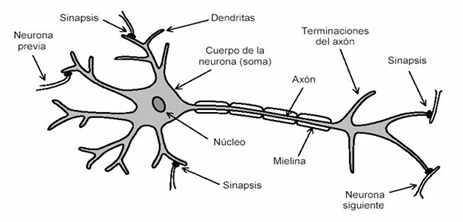
\includegraphics[width=10.5cm]{Sources/neurona.png}
	\captionof{figure}{Neurona biológica}
\end{floatingfigure}

El elemento estructural y funcional más esencial, en el sistema de comunicación neuronal, es la célula nerviosa o neurona. La mayoría de las neuronas utilizas sus productos de secreción como señales químicas (transmisores) para la transmisión de información. Dicha información se envía, entre las distintas neuronas, a través de prolongaciones, formando redes en las cuales se elabora y almacena información.

La misión de las neuronas comprende generalmente cinco funciones parciales:

{\setlength{\baselineskip}{0.7\baselineskip}\begin{itemize}
	\item Las neuronas recogen la información que llega a ellas en forma de impulsos procedentes de otras neuronas o de receptores.
	\item La integran en un código de activación propio de la célula.
	\item La transmiten codificada en forma de frecuencia de impulsos a través de su axón. 
	\item A través de sus ramificaciones el axón efectúa la distribución espacia de los mensajes.
\end{itemize}}

Una Red de Neuronas Artificiales (en adelante, RNA) es un paradigma de procesamiento de información inicialmente inspirado en el modo en el que lo hace el cerebro. El elemento clave de este paradigma es su estructura. Las RNA están compuestas por un cierto número de elementos de procesamiento o neuronas que trabajan al unísono para resolver un problema específico. 

\begin{wrapfigure}{l}{6.1cm}
	\vspace{0.2cm}
		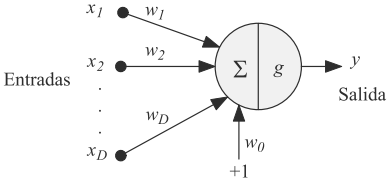
\includegraphics[width=6cm]{Sources/modelo_neurona.png}
		\captionsetup[figure]{margin=0.3cm, justification=centering}
		\captionof{figure}{Modelo matemático de una neurona}\label{modeloneurona}
\end{wrapfigure}

Las redes neuronales actuales se basan en el modelo matemático de neurona propuesto por \textit{McCulloch} y \textit{Pitts} en 1943. En dicho modelo (véase Figura \ref{modeloneurona} ) cada neurona recibe un conjunto de entradas ${x1, x2,...,xD}$ y devuelve una única salida . Además, dentro de una RNA existen numerosas conexiones entre las distintas neuronas que la forman. Estas conexiones simulan las conexiones neuronales del cerebro y, al igual que éstas, pueden establecerse con mayor o menor intensidad. En el caso de las RNA esta intensidad la determinan los pesos sinápticos (o simplemente pesos). De este modo, cada entrada $x_i$ de una neurona se encuentra afectada por un peso $w_i$.

El primer paso para obtener la salida de la neurona es calcular la suma ponderada $a$ de las entradas, llamada activación de la neurona:
$$a = \displaystyle \sum_{i=1}^{D} w_ix_i + w_0$$
Donde w0 es un umbral o sesgo que se utiliza para compensar la diferencia entre el valor medio de las entradas, sobre todo el conjunto de entrenamiento, y el correspondiente valor medio de las salidas deseadas. Posteriormente, a partir de este valor a se obtiene la salida y de la neurona mediante la aplicación de una función, llamada función de activación o de transferencia g(a), es decir:
$$y = g(a) = g\left( \sum_{i=1}^{D}w_ix_i+w_0\right) = g\left( \sum_{i=0}^{D}w_ix_i \right) $$
Donde, como se observa, es posible tratar el umbral $w_0$ como un peso más si se supone una entrada añadida $x_0$ con un valor fijo de 1. Finalmente, también es posible reescribir esta ecuación en notación vectorial como $g(a) = g(w^T x)$, si tomamos $w$ como el vector de pesos y $x$ como el vector de entradas a la red. La función de transferencia empleada en este modelo básico de \textit{McCulloch-Pitts} es la función escalón definida por la ecuación: 
$$\displaystyle g(a) = \left\{ { 0 \mbox{ cuando } x < 0  \atop 1 \mbox{ cuando } a > 0 } \right.$$

En los modelos actuales se escogen otro tipo de funciones, normalmente monótonas y derivables. A continuación se presentarán algunas de ellas.

{\setlength{\baselineskip}{0.7\baselineskip}\begin{itemize}
	\item lineal $g(a)=a$
	\item sigmoidal $g(a) = \displaystyle \frac{1}{1 +e^{-a}}$
	\item tangente hiperbólica $g(a)= \displaystyle \frac{e^a -e^{-a}}{e^a + e^{-a}}$
	\item gaussiana $g(a) = e\left( \displaystyle -\frac{(a-\mu)^2}{2\sigma^2} \right) $
\end{itemize}}

\begin{figure}[H]
	\centering
	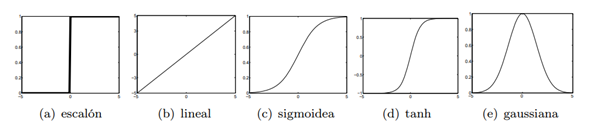
\includegraphics[width=0.8\linewidth]{Sources/funciones_activacion.png}
	\caption{Funciones de activación}
\end{figure}

\subsubsection{Algoritmos genéticos}
Los Algoritmos Genéticos (AG) fueron introducidos inicialmente por Holland en 1975 para abstraer y explicar rigurosamente los procesos adaptativos de los sistemas naturales, así como para el diseño de sistemas artificiales de software que retengan los mecanismos importantes de los sistemas naturales. Fue unos años más tarde cuando su alumno, D. Goldberg, implementó el primer AG aplicado en problemas industriales. Estas y otras aplicaciones creadas por estudiantes de Holland convirtieron los AGs en un campo suficientemente aceptado.

En un AG, las soluciones potenciales al problema se representan normalmente mediante cadenas binarias de bits (0’s y 1’s) de una longitud determinada \emph{long} que vendrá impuesta por el número de variables existentes en la solución y por el número de bits necesarios para codificarlas. Otros términos usados a menudo para denominar una solución del problema en un AG son string o estructura, y, siguiendo el vocabulario de los sistemas biológicos, cromosoma.

Así, los cromosomas están compuestos por unidades binarias que se denominan genes. Al valor de un gen determinado se le denomina alelo, y a su posición en el cromosoma locus. Al paquete genético total se le denomina genotipo, y a la interacción del genotipo con su entorno se le denomina fenotipo, que se traduce en la decodificación del cromosoma para la obtención de una solución alternativa (conjunto de parámetros particulares, o un punto en el espacio de búsqueda). De esta forma, podemos representar un cromosoma $c_i^t$ en una generación (iteración) determinada $t$ como:
{\large $$ c_i^t = \displaystyle (b_{i_1}^t \ldots b_{i_long}^t)$$}
Con $b_{i_j}^t$ $\in$ \{0, 1\}, $j$ = 1,$\ldots$, $long$. El término individuo es frecuentemente utilizado para referirse al conjunto de información genotipo-fenotipo adecuación. Así, podemos representar un individuo $X_i^t$ en una generación $t$, como la terna:
{\large $$ X_i^t = \displaystyle (c_i^t, x_i^t, f_i^t)$$}
Donde $X_i^t$ es la decodificación (fenotipo) del cromosoma $c_i^t$, y $f_i^t$ es la adecuación de la solución al entorno o \textit{fitness}.

\subsubsection{Sistemas expertos}

En la década de los setenta se inicia la explosión de aplicaciones de la IA en términos de sistemas basados en reglas a los que se les llama primero “Sistemas Expertos” y después “Sistemas Basados en Conocimiento”. El reconocimiento de la insuficiencia de la lógica como herramienta única de representación da lugar al desarrollo de otras formas de representación e inferencia mediante redes causales y asociativas (semánticas, neuronales y bayesianas) y marcos, objetos y agentes.

El área de sistemas expertos es una aproximación muy exitosa a la solución de problemas clásicos de AI en la programación de inteligencia. El profesor Edward Feigenbaum de la Universidad de Stanford, pionero en la tecnología de los sistemas expertos, los ha definido como “un programa de computación inteligente que usa el conocimiento y procedimientos de inferencia para resolver problemas que son lo suficientemente difícil como para requerir significativa experiencia humana para su solución, es decir, un sistema experto es un sistema de cómputo que emula la habilidad de tomar decisiones de un especialista humano.

El conocimiento de un sistema experto puede representarse de varias maneras (puede estar encapsulado en reglas y objetos). Un método común de representar el conocimiento es en forma de reglas tipo SI…ENTONCES, como:
\begin{center}
	\textit{SI la luz es roja ENTONCES deténgase.}
\end{center}
Aunque se trata de un ejemplo muy simple, se han construido muchos sistemas expertos significativos expresando en reglas el conocimiento de especialistas.

Los sistemas expertos se han aplicado casi a todos los campos del conocimiento, debido a eso a continuación se mencionarán algunos:


\begin{longtable}[c]{lll} \toprule
	Nombre del S.E.& Área & Descripción\\\midrule
	SPEX & Química & Planear experimentos de biología molecular. \\
	PUFF & Medicina & Diagnosticar enfermedades de los pulmones. \\
	LITHO & Geología & Interpretar los datos de registro de pozos petroleros.\\
	TIMM & Informática & Diagnosticar computadoras DEC.\\\bottomrule
	\caption{Ejemplos de Sistemas Expertos}
\end{longtable}


\subsection{Lógica difusa}\label{seccion:logicadifusa}
Hace más de 50 años, en 1965 Lotfi A. Zadeh, en aquel entonces director del Departamento de Ingeniería Eléctrica de la
Universidad de California en Berkeley, publicó \emph{Fuzzy Sets}. Este artículo describe las matemáticas de los
conjuntos difusos y por extensión de la lógica difusa, y este trabajo le dio nombre a su campo. Zadeh
aplicó la lógica de Lukasiewicz a cada objeto en un conjunto y creó un álgebra completa para conjuntos
difusos. Esta teoría propone \emph{funciones de pertenencia} (o los valores falso y verdadero) sobre el rango
[0.0, 1.0]. 

El ser humano muestra dificultad para tomar decisiones cuando
se tiene información imprecisa. La lógica difusa fue creada para emular la lógica humana y tomar decisiones
acertadas a pesar de la información. Es una herramienta flexible que se basa en reglas lingüísticas
dictadas por expertos. Por ejemplo, la velocidad de un automóvil es una variable que puede tomar distintos
valores lingüísticos, como “alta”, “media” o “baja”. Estas variables lingüísticas están regidas por
reglas que dictan la salida del sistema.
En otras palabras, la lógica difusa es un conjunto de principios matemáticos basados en \emph{grados de
membresía o pertenencia}, cuya función es modelar información. Este modelado se hace con base en
reglas lingüísticas que aproximan una función mediante la relación de entradas y salidas del sistema
(composición). Esta lógica presenta rangos de membresía dentro de un intervalo entre 0 y 1, a diferencia
de la lógica convencional, en la que el rango se limita a dos valores: el cero o el uno.




\subsection{Conjuntos difusos}

El concepto de conjunto difuso fue propuesto por Zadeh(1965): ``Un conjunto difuso es una colección de objetos con un \textit{grado de membresía} continuo. Un conjunto tal, es caracterizado por una \textit{función de membresía} que asigna a cada objeto un grado de membresía en un rango de 0 a 1.'' (p.338).

En teoría clásica de conjuntos, un conjunto tiene unos límites \textit{nítidos} bien definidos (límites \textit{crisp}). Por ejemplo, el conjunto A de los números más grandes que 8 se representa como:

\begin{displaymath}
	A = \lbrace  x \ | \ x > 8 \rbrace
\end{displaymath}

Sin embargo, los conceptos manejados por el ser humano como \textit{frío} y \textit{caliente}, tienen una transición gradual. Así, un conjunto difuso, lidia con la vaguedad inherente de estos conceptos, conteniendo los elementos sólo con un cierto grado de pertenencia.
 
En teoría de conjuntos difusos, los conceptos se asocian a conjuntos difusos (asociando sus \emph{valores de pertenencia}) en un proceso llamado \emph{fuzzificación}. Una vez que tenemos los valores \emph{fuzzificados} podemos trabajar con \emph{reglas lingüísticas} y obtener una salida, que podrá seguir siendo difusa o \emph{defuzzificada} para obtener un valor discreto.

Sea $X$ el \emph{Universo del discurso}, y sus elementos se denotan como $x$; En la teoría clásica de conjuntos se define un conjunto $C$ sobre $X$ mediante la \emph{función característica} de $C$ como $f_c$ .

$$\displaystyle f_c(x) = \left\{ { 1 \mbox{ cuando } x \in C  \atop 0 \mbox{ cuando } x \notin C } \right.$$

Este conjunto mapea el universo $X$ en un conjunto de dos elementos,
donde la función $fc (x)$ es $1$ si el elemento $x$ pertenece al conjunto
$C$ y $0$ si el elemento $x$ no pertenece al conjunto $C$.

Si generalizamos esta función para que los valores asignados a los
elementos del conjunto caigan en un rango particular y así indicar
el grado de pertenencia de los elementos a ese conjunto, tendremos
una \textbf{función de pertenencia} de un determinado conjunto difuso.
La función de pertenencia $\mu_A $ por la que se define un conjunto difuso $A$,
Sería:

\begin{displaymath}
\mu_A = X \rightarrow \left[ 0,1 \right]
\end{displaymath}


Donde $\mu_A(x) = 1$ si $x$ está totalmente en $A$,
$\mu_A(x) = 0$ si $x$ no está en $A$
y $ 0 < \mu_A(x) < 1 $ si $x$ está parcialmente en $A$.
Este valor entre 0 y 1 representa el grado de pertenencia $\mu$ al conjunto $A$.


\textit{Definición formal}\\
Un conjunto difuso $A$ definido en el universo de discurso $U$ es caracterizado por una función de membresía $\mu_A : U \rightarrow [0,1]$ que asocia a cada elemento $u$ de $U$ un valor $\mu_A(u)$ en el intervalo [0,1], con $\mu_A(u)$ representando el grado de membresía de $u$ en $A$.

Algunas características:
{\setlength{\baselineskip}{0.7\baselineskip}\begin{description}
	\item El soporte de A son los puntos en $U$ en los cuales $\mu_A(u)$ es positivo.
	\item La altura de A es el valor máximo de $\mu_A(u)$ sobre $U$.
	\item El punto de cruce de A es un punto en $U$ donde el valor de membresía en $A$ es $0.5$
\end{description}}





\subsubsection{Principio isomorfo}

Es bien conocido que la teoría de conjuntos, el \textit{Álgebra booleana} y la Lógica tradicional son isomorfas, bajo transformaciones adecuadas. Esto significa que tienen una estructura subyacente similar, y que por tanto, las definiciones que se hagan en una de las tres teorías se pueden llevar a las otras dos, mediante las transformaciones adecuadas.
En el siguiente cuadro se muestra la correspondencia de algunos operadores.\\\\


\begin{longtable}{|c|c|c|} 
	\hline
	Teoría de conjuntos & Álgebra booleana & Lógica tradicional \\ \hline
	Intersección & Conjunción & AND \\ \hline
	Unión & Disyunción & OR \\ \hline
	Complemento & Negación & NOT \\ \hline
	\caption{Correspondencia entre operadores} \label{table:tblop}
\end{longtable}

Ahora bien, el razonamiento lógico consiste en la combinación de proposiciones para producir nuevas proposiciones; así, la combinación de las proposiciones \textit{X es A} y  \textit{Y es B} mediante el operador \textit{AND} da como resultado la proposición \textit{X es A AND Y es B}. El cuadro \ref{table:tblop} sugiere que puede representarse esta combinación mediante un operador análogo a la intersección de conjuntos.

Lo anterior es posible porque en lógica tradicional toda proposición puede tener uno de dos valores, \textit{verdadero} o \textit{falso}, lo que corresponde en la teoría de conjuntos discretos a los únicos dos valores que puede tomar la función de pertenencia para cualquier conjunto: 1 ó 0.


Ahora bien, en lógica difusa una proposición puede representarse por un conjunto difuso \textit{X es A} corresponde a un conjunto A con función de pertenencia $\mu_A(x)$, mientras \textit{Y es B} corresponde a un conjunto B con función de pertenencia $\mu_B(x)$, y la combinación de estas dos proposiciones con el operador \textit{AND}, es decir, la proposición \textit{X es A AND Y es B} corresponde a un nuevo conjunto difuso \textit{A AND B} con función de pertenencia:

\begin{displaymath}
\mu_{A \cap B}(x,y) =  \min(\mu_A(x),\mu_B(y))
\end{displaymath}

En donde se ha utilizado el operador $\min$ parara efectuar la intersección de los dos conjuntos, pero en general podría haberse utilizado cualquier norma T.

Nótese que los universos de discurso sobre los cuales están definidos los conjuntos A y B no son necesariamente el mismo; son, por ejemplo U y V respectivamente, mientras el conjunto $A \cap B$ está definido sobre el universo $U \times V$.

En forma análoga, al operador lógico $OR$ puede hacerse corresponder a una \textit{norma S}, mientras al operador lógico $NOT$ puede hacerse corresponder el complemento.









\subsection{Operaciones de conjuntos difusos}

Las tres operaciones básicas entre conjuntos discretos: \emph{unión, intersección y complemento}, se definen también para los conjuntos difusos, intentando mantener el significado de tales operaciones. La definición de estas operaciones se hace empleando el concepto de función de pertenencia de los conjuntos.

\subsubsection{Intersección}

Dado dos conjuntos difusos $A$ y $B$ con funciones de pertenencia $\mu_A(x)$ y $\mu_B(x)$, respectivamente.
La intersección $A \cap B$ puede representarse en general como una función
$T:[0,1] \times [0,1] \rightarrow [0,1]$ o como un operador binario $\vartriangle$, tal que:

%La intersección es un nuevo conjunto difuso $A \cap B$ con una función de pertenencia:

\begin{displaymath}
\mu_{A \cap B}(x,y) = T [ \mu_A(x), \mu_B(y) ] = \mu_A(x) \vartriangle \mu_B(y)
\end{displaymath}

Donde $T$, debe satisfacer las siguientes propiedades:

\begin{enumerate}
	\item \textsl{Elemento unidad:} $T(a,1) = a$ y $T(a,1)=T(1,a)=a$
	\item \textsl{Conmutatividad:} $T(a,b) = T(b,a)$
	\item \textsl{Monotonicidad:} Si $a \leq c$ y $b \leq d$ entonces $T(a,b) = T(c,d)$
	\item \textsl{Asociatividad:} $T(T(a,b),c) = T(a,T(b,c))$
\end{enumerate}

Todo operador que satisfaga las propiedades anteriores se conoce como una \textbf{Norma Triangular} o \textbf{Norma T} y representa la intersección de dos conjuntos difusos. Algunas \textit{normas T} ampliamente utilizadas son:

\begin{itemize}
	\item \textsl{Mínimo:} $T_{min}(a,b) = min(a,b)$
	\item \textsl{Producto algebraico:} $T_{ap}(a,b) = ab$
	\item \textsl{Diferencia limitada (o de Lukasiewick)}: $T_{bp}(a,b) = max(0, a+b-1)$
\end{itemize}





\subsubsection{Unión}
Dado dos conjuntos difusos $A$ y $B$ con funciones de pertenencia $\mu_A(x)$ y $\mu_B(x)$, respectivamente.
La unión $A \cup B$ puede representarse en general como una función
$S:[0,1] + [0,1] \rightarrow [0,1]$ o como un operador binario $\bot$, tal que:

%Dado nuevamente, dos conjuntos difusos $A$ y $B$, con funciones de pertenencia $\mu_A(x)$ y $\mu_B(x)$, respectivamente. La unión se define como un nuevo conjunto difuso $A \cup B$ con una función de pertenencia:

\begin{displaymath}
\mu_{A \cup B}(x,y) = S \left[ \mu_A(x), \mu_B(y) \right] = \mu_A(x) \ \bot \ \mu_B(y)
\end{displaymath} 

Donde $S$, debe satisfacer las siguientes propiedades:

\begin{enumerate}
	\item \textsl{Elemento Neutro:} $S(1,1)=1$ y $S(a,0) = S(0,a) = a$
	\item \textsl{Conmutatividad:} $S(a,b) = S(b,a)$
	\item \textsl{Monotonicidad:} Si $a \leq c$ y $b \leq d$ entonces $S(a,b) = S(c,d)$
	\item \textsl{Asociatividad:} $S(S(a,b),c) = S(a,S(b,c))$
\end{enumerate}


Todo operador que satisfaga las propiedades anteriores se conoce como una \textbf{Conorma T} o \textbf{Norma S} y representa la unión de dos conjuntos difusos. Algunas \textit{normas S} ampliamente utilizadas son:

\begin{itemize}
	\item \textsl{Máximo:} $S_{max}(a,b) = max(a,b)$
	\item \textsl{Producto:} $S_{as}(a,b) = (a+b) - (a \times b)$
	\item \textsl{Suma limitada (o de Lukasiewick)}: $S_{bs}(a,b) = min(a+b,1)$
\end{itemize}

\subsubsection{Complemento}
Dado un conjunto $A$, con función de pertenencia $\mu_A(x)$.
El complemento $\neg A$ puede generalizarse considerándolo como una función
$N:[0,1] \rightarrow [0,1]$, tal que:


\begin{displaymath}
	\mu_{\neg A}(x) = N( \mu_A(x) )
\end{displaymath}

La operación de complemento, a la que llamaremos \textbf{Norma N}, también debe cumplir ciertas propiedades:

\begin{enumerate}
	\item \textsl{Condición limite o frontera:} $N(0) = 1$ y $N(1) = 0$.
	\item \textsl{Monotonicidad:} si $a \leq b$ entonces $N(a) \geq N(b)$.
	\item \textsl{Continuidad:} la función de complemento $N(a)$ es continua.
	\item \textsl{Involutividad:} $N(N(a)) = a $
\end{enumerate}

Al igual que con la unión y la intersección, también para el complemento, existen gran variedad de clases.
Algunas \textit{normas N} más utilizadas son:

\begin{enumerate}
	\item \textsl{Clásico:} $N_{c}(a) = 1 - a$
	\item \textsl{Sugeno:} $N_{s}(a) = \frac{1-a}{1+sa}$ con $s \in (-1,\infty)$
	\item \textsl{Yager:} $N_{w}(a) = (1-a^w)^{1/w}$ con $w \in (0, \infty)$
\end{enumerate}



\subsection{Funciones de membresía}\label{cap:membershipfunction}

Para definir un conjunto difuso $A$, hay que definir su \textit{función de membresía} o \textit{función de pertenencia}.
Supongamos una función de pertenencia: $\mu_A(x)$, la imagen de la función es la curva que define el grado de pertenencia de cada elemento $x$ al conjunto $A$.

Para la correcta representación de los grados de pertenencia de cada uno de los elementos que conforman el conjunto difuso, lo más natural es extraer los datos de los fenómenos que se va a representar y con ellos, elegir y ajustar una función de membresía adecuada. De otra manera existen metodologías que permiten asignar grados de membresía a cada uno de los elementos del conjunto.

Algunas de las funciones de membresía básicas son las siguientes.

\paragraph{Triangular.}
\begin{wrapfigure}{r}{0pt}
	\begin{tikzpicture}
		\draw[->] (0,0) -- (4,0) 	node[right] {$x$} 		coordinate (x axis);
		\draw[->] (0,0) -- (0,1) 	node[above]	{$\mu(x)$} 	coordinate (y axis);
		\draw[blue,semithick] (0,0) -- (1,0) node[above] {a} -- (2,1) node[above] {b} -- (3,0) node[above] {c} -- (4,0);
	\end{tikzpicture}
	\captionsetup{margin=1cm,justification=centering}	
	\caption{Función triangular}
	\label{fig:trimf}
\end{wrapfigure}
La imagen de la función, como su nombre lo indica, asemeja un triángulo. Realmente la función está compuesta por dos líneas rectas, una con pendiente positiva hasta alcanzar la unidad, y otra con pendiente negativa, hasta llegar a 0. Está definida por tres parámetros \textit{a, b, c} donde $ a \leq b \leq c$. Estos parámetros definen los vértices de la función.\\\\
Su definición matemática es la siguiente:
$$  f(x;a,b,c)= \left\lbrace \begin{array}{lcl}
0	& \mbox{si} & x  \leq a \\ [.30cm]
{\displaystyle \frac{x-a}{b-a}} & \mbox{si} & a \leq x \leq b \\ [.45cm]
%{\scriptstyle (x-a)/(b-a)} & \mbox{si} & a \leq x \leq b \\ [.15cm]
{\displaystyle \frac{c-x}{c-b}} & \mbox{si} & b \leq x \leq c \\ [.45cm]
%{\scriptstyle (c-x)/(c-b)} & \mbox{si} & b \leq x \leq c \\ [.15cm]
0 & \mbox{si} & x \geq c \\
\end{array}				
\right.
$$

La función triangular es adecuada para definir situaciones en las que se tiene un valor óptimo central, el cual se va perdiendo conforme se aleja de él. Un ejemplo de esta situación es la temperatura corporal, esta tiene un valor óptimo de $36\,^{\circ}\mathrm{C}$, pero por debajo de $35\,^{\circ}\mathrm{C}$ o por encima de $37\,^{\circ}\mathrm{C}$ se podría considerar peligrosa.


\paragraph{Trapezoidal.}
\begin{wrapfigure}{r}{0pt}
	\begin{tikzpicture}
		\draw[->] (0,0) -- (4,0) 	node[right] {$x$} 		coordinate (x axis);
		\draw[->] (0,0) -- (0,1) 	node[above]	{$\mu(x)$} 	coordinate (y axis);		
		\draw[blue,semithick] (0,0) -- 	(1  ,0)	node[above] {a} --
		(1.5,1) node[above] {b} --
		(2.5,1)	node[above] {c} --
		(3,0)	node[above] {d} --
		(4,0);
	\end{tikzpicture}
	\captionsetup{margin=1cm,justification=centering}	
	\caption{Función triangular}
	\label{fig:trapmf}
\end{wrapfigure}

Una generalización de la función triangular es la función trapezoidal, que a diferencia de la triangular, tiene un núcleo más amplio. Esto es, el intervalo donde el valor de membresía es igual a 1 se extiende entre los vértices
$b$ y $c$.
La función está definida por cuatro parámetros \textit{a, b, c, d} donde $ a \leq b \leq c \leq  d$. En la figura \ref{fig:trapmf} se aprecia el trapecio que forman estos cuatro vértices.\\\\
Su definición matemática es la siguiente:

$$  f(x;a,b,c,d)= \left\lbrace \begin{array}{lcl}
						0		& \mbox{si} & x  \leq a \\ [.30cm]
{\displaystyle \frac{x-a}{b-a}} & \mbox{si} & a \leq x \leq b \\ [.45cm]
						1		& \mbox{si} & b \leq x \leq c \\ [.30cm]
{\displaystyle \frac{c-x}{c-b}} & \mbox{si} & c \leq x \leq d \\ [.45cm]
						0 		& \mbox{si} & x \geq d \\
\end{array}
\right.
$$

La forma de esta función es utilizada cuando hay un rango de valores óptimos. Un ejemplo de esto es la temperatura ambiente. Hay un rango de temperaturas que podemos considerar adecuadas, pero por debajo de este rango las personas comienzan a sentir frío, y por encima de él se consideraría un ambiente caluroso.


\paragraph{Gaussiana.}
\begin{wrapfigure}{r}{0pt}
	\begin{tikzpicture}[domain=0:8, xscale=0.5]
	\draw[->] (0,0) -- (8,0) 	node[right] {$x$} 		coordinate (x axis);
	\draw[->] (0,0) -- (0,1) 	node[above]	{$\mu(x)$} 	coordinate (y axis);
	
	\draw[blue, semithick]	plot(\x,{  exp( -1/2 * pow( ( (\x - 4) / 1 ) ,2) ) });
	\draw[blue] (4,1) node[above] {$x_0$};
	\draw[blue] (5.6,0.3) node[above] {$\sigma$};
	
	\end{tikzpicture}
	\captionsetup{margin=1cm,justification=centering}	
	\caption{Función gaussiana}
	\label{fig:gaussmf}
\end{wrapfigure}

La \textit{función gaussiana} es una función simétrica que juega el papel de la función triangular, solo que esta pertenece al grupo de las funciones con derivada continua. Si observamos la figura \ref{fig:gaussmf} podemos ver como la gráfica asemeja un triángulo suavizado, es decir, los vértices no tienen cambios abruptos sino graduales.\\\\
Su definición matemática es la siguiente:
\begin{displaymath}
f(x;a,x_0)=  e^{\displaystyle -\frac{1}{2} \left(  \frac{x-x_0}{a} \right)^2 }
\end{displaymath}
Donde
{\setlength{\baselineskip}{0.7\baselineskip}\begin{description}
	\item $x_0$ determina el centro o punto de cruce y,
	\item $a$ determina el ancho o la pendiente.
\end{description}}

%test campana generalizada
\paragraph{Campana generalizada.}

\begin{wrapfigure}{r}{0pt}
		\begin{tikzpicture}[domain=0:8, xscale=0.5]
			\draw[->] (0,0) -- (8,0) 	node[right] {$x$} 		coordinate (x axis);
			\draw[->] (0,0) -- (0,1) 	node[above]	{$\mu(x)$} 	coordinate (y axis);
			
			\draw[blue, semithick]	plot(\x,{ 1 / ( 1 + pow( (\x - 4)/ 1.5 , 2 * 2) ) });
			\draw[blue] (4,1) node[above] {$x_0$};
			\draw[blue] (4,1) node[above] {$x_0$};
			\draw[blue] (5.6,0.3) node[above] {$\sigma$};
		\end{tikzpicture}
		\captionsetup{margin=1cm,justification=centering}	
		\caption{Función Campana generalizada}
		\label{fig:gbellmf}
\end{wrapfigure}
Esta función al igual que la anterior, es una función simétrica con derivada continua. Juega el papel de una función trapezoidal, si observamos la figura \ref{fig:gbellmf}, podemos ver como la gráfica asemeja un trapecio suavizado, es decir, los vértices no tienen cambios abruptos sino graduales.\\\\
Su definición matemática es la siguiente:

\begin{displaymath}
f(x;a,b,x_0)= \frac{1}{1 + \left(  \frac{x-x_0}{a}  \right)^{2b}}
\end{displaymath}
Donde
{\setlength{\baselineskip}{0.7\baselineskip}\begin{description}
	\item $x_0$ determina el centro o punto de cruce,
	\item $a$ determina el ancho y,
	\item $b$ determina la pendiente.
\end{description}}


\paragraph{Sigmoidal.}

\begin{wrapfigure}{r}{0pt}
	\begin{tikzpicture}[domain=0:8, xscale=0.5, yscale=1]
		\draw[->] (0,0) -- (8,0) 	node[right] {$x$} 		coordinate (x axis);
		\draw[->] (0,0) -- (0,1) 	node[above]	{$\mu(x)$} 	coordinate (y axis);
		\draw[blue]	plot(\x,{ 1 / ( 1 + exp( -1 * -2 * (\x-3.5)  ) ) });
	\end{tikzpicture}
	\captionsetup{margin=1cm,justification=centering}	
	\caption{Función Sigmoidal}
	\label{fig:sigmf}
\end{wrapfigure}

Una sigmoidal es una función con derivada continua y abierta. Su gráfica recuerda la forma de un escalón. Tiene un parámetro $a$ que determina su pendiente, es decir, determina la suavidad de la transición entre los valores de membresía 0 a 1. Además el parámetro a también determina si la función abrirá por la izquierda o por la derecha. Un valor positivo de $a$ genera un gráfica abierta por la derecha
y un valor negativo genera que l gráfica se abra por la izquierda.
En la imagen \ref{fig:sigmf} podemos observar una función sigmoidal abierta por la izquierda.\\\\
Su definición matemática es la siguiente:
\begin{displaymath}
	f(x;a,x_0) = \frac{1}{1+e^{-a(x-x_0)}}
\end{displaymath}
Donde
{\setlength{\baselineskip}{0.7\baselineskip}\begin{description}
	\item $x_0$ determina el centro o punto de cruce y,
	\item $a$ determina la pendiente.
\end{description}}

\subsection{Variables lingüísticas}
Una variable lingüística adopta términos lingüísticos que permiten describir el estado de un objeto o fenómeno usando un lenguaje natural(o artificial); estos términos se pueden representar mediante conjuntos difusos. Una variable numérica toma valores numéricos, por ejemplo: \textit{carros = 2}, mientras que una variable lingüística toma valores lingüísticos: carros es \textit{``pocos''}.

De manera más formal: Los valores de una variable lingüística $X$ son las etiquetas $T(x)$ de los subconjuntos difusos en U(conjunto universo). Las etiquetas pueden tener la forma de frases o sentencias en lenguaje natural o artificial. Por ejemplo, si U es la colección de enteros correspondiente a las edades de un grupo de personas:
$$U = 10 + 1 + 2 + ... + 70$$
y la edad es una variable lingüística llamada \textit{x} definida en \textit{U}, entonces los valores de \textit{x} podrían ser \textit{niño, joven, adulto joven, adulto, anciano}, etc. Donde los posibles valores son las etiquetas de los conjuntos difusos que caracterizan las edades (véase la fig. \ref{fig:variableling}).

\begin{figure}[!h]
	\centering
	\begin{tikzpicture}[yscale=2, xscale=1.5]
		\draw[->] (1,0) -- (7,0) 	node[right] {${\scriptstyle x}$} 		coordinate (x axis);
		\draw[->] (1,0) -- (1,1) 	node[left]	{${\scriptstyle \mu(x)}$} 	coordinate (y axis);
		
		\foreach \x in {1, 2, ..., 7}
			\draw[xshift=\x cm] (0pt,1pt) -- (0pt,-1pt) node[below] {{\scriptsize \x0}};
		
		
		\draw[blue, semithick] (1,1) node[above=5pt] {niño} -- (2.5,0);
		\draw[black, semithick]	(1,0) -- (2.5,1) node[above=5pt] {joven} -- (4,0);
		\draw[red,semithick] (2.5,0) -- (4,1) node[above=5pt] {adulto joven}  -- (5.5,0);
		\draw[orange,semithick] (4,0) -- (5.5,1) node [above=5pt] {adulto} -- (7,0);
		\draw[purple,semithick] (5.5,0) -- (7,1) node [above=5pt] {anciano} -- (7,0);
	\end{tikzpicture}
	\caption{Variable lingüística \emph{edad} llamada $x$}
	\label{fig:variableling}
\end{figure}

El significado de un término lingüístico $T(x)$ es caracterizado mediante una \textit{función de compatibilidad o membresía}: $C : U \rightarrow [0,1]$, la cual, asocia la compatibilidad (o grado de pertenencia) de cada $u$ en $U$, con $T(x)$. Así, la compatibilidad de una edad de \textit{27 años} con el término lingüístico \textit{joven} podría ser 0.7, mientras que una edad de \textit{35 años} podría ser de 0.2.

El concepto de variable lingüística proporciona un medio para definir de manera aproximada los fenómenos que son demasiado complejos o muy imprecisos como para ser receptivos de una descripción convencional en términos cuantitativos.

Una variable lingüística está caracterizada mediante la quíntupla:
$$(X,T(x),U,G,M)$$
Donde
{\setlength{\baselineskip}{0.7\baselineskip}\begin{description}
	\item $X$ es el nombre de la variable.
	\item $T(X)$ es el conjunto de términos o valores lingüísticos.
	\item $U$ es el universo de discurso.
	\item $G$ es la regla sintáctica que genera los términos en $T(x)$; y,
	\item $M$ es una regla semántica que socia cada valor lingüístico $X$ con su correspondiente significado $M(X)$, siendo $M(X)$ un conjunto difuso en $X$.
\end{description}}

Hay varios aspectos básicos que es necesario tomar en cuenta al momento de definir de una variable lingüística.

Primero, Es importante entender que la noción de membresía es distinta a la de probabilidad. Así, la declaración de que la membresía de la edad de \emph{28 años} al conjunto difuso \emph{joven} es de 0.7, no tiene relación con la probabilidad de que la edad sea o no 28.
La interpretación correcta es que el valor de membresía 0.7, es simplemente una indicación subjetiva de \emph{qué tanto encaja} la edad de ``28 años'' (\textit{en una escala de 0 a 1}) con el concepto ``joven''.
%La interpretación correcta del valor de membresía 0.7, es que, simplemente es una indicación subjetiva de \emph{en qué grado} (\textit{en una escala de 0 a 1}) la edad de ``28 años'' encaja en el concepto ``joven''.

Segundo, normalmente asumiremos que una variable lingüística está \emph{estructurada} tomando en cuenta dos reglas:
\begin{description}
	\item[Regla (i).] La regla sintáctica, esta especifica la manera en que se generan los términos lingüísticos de la variable.
	En relación a esta regla, normalmente asumiremos que los términos de la variable son generados por una gramática de contexto libre.
	\item[Regla(ii).] La regla semántica, que especifica el proceso para computar el significado de cualquier término lingüístico dado. Aquí, observamos que un valor típico de una variable lingüística involucra lo que llamamos términos primarios (joven y viejo) que son a su vez, subjetivos y dependientes de contexto. Por lo que se asume que el significado de dichos términos es conocido \emph{a priori}.
\end{description}

En resumen, al momento de definir una variable lingüística $(X,T(x),U,G,M)$, se asume que $G$ es una gramática libre de contexto, además que,
cualquier significado $M(x)$  generado por $M$ es subjetivo y conocido \emph{a priori}. Por lo que normalmente $M$ y $G$ se omitirán en la definición.

Tomando en cuenta lo anterior, una variable lingüística se define básicamente por la siguiente tripla.
$$(X,T(x),U)$$
Donde:
{\setlength{\baselineskip}{0.7\baselineskip}\begin{description}
	\item $X$ es el nombre de la variable.
	\item $T(x)$ es el conjunto de términos o valores lingüísticos.
	\item $U$ es el universo de discurso.
\end{description}}


 
\subsection{Sistema difuso}
Un sistema de inferencia difuso (\textit{FIS}) consta, conceptualmente, de tres etapas. En la primer etapa se transforman (fuzzifican) las variables de entrada obteniendo valores de difusos. Posteriormente dichos valores son manejados por un sistema de inferencia que genera una salida, también difusa, a partir de las reglas establecidas y los propios valores de entrada. Finalmente el resultado pasa por un proceso llamado defuzzificación, a través del cual, se obtiene la salida real del sistema ya en valores concretos. La figura \ref{fig:digfis} muestra el diagrama esquemático del controlador
difuso.

\begin{figure}[H]
	\centering
	\begin{tikzpicture}[scale=2]
	
	\node[draw,rectangle] (fl) at (0,0) {Reglas difusas};
	\node[draw,rectangle] (fz) [left= of fl] {Fuzzificador};
	\node[draw,rectangle] (df) [right= of fl] {Defuzzificador};
	\node[draw,rectangle] (fe) [below= of fl] {Motor de inferencia};
	
	\path (fl) edge[<->] (fe);
	\path (fz) edge[->] (fl);
	\path (fl) edge[->] (df);
	\end{tikzpicture}
	
	\caption{Diagrama esquemático de un sistema de inferencia difuso}
	\label{fig:digfis}
\end{figure}



\subsubsection*{Fuzzificación}
La primera etapa se basa en un proceso donde las variables tienen un grado de incertidumbre metalingüístico. Por lo tanto, el rango de valores (\textit{universo de discurso}) de cada variable puede clasificarse por conjuntos difusos\footnote{Para más información véase la sección \ref{cap:membershipfunction} \textit{Funciones de membresía}.}, por ejemplo \textit{baja, media, alta}.
Cuando el sistema obtiene variables, pasan por un proceso de \textit{fuzzificación}
que consiste en pasar dichos valores a un rango de pertenencia entre cero (0) y uno (1).
Se busca determinar el grado de pertenencia del valor de entrada a un conjunto difuso.
Los conjuntos difusos son caracterizados mediante funciones de membresía ajustadas a las necesidades del sistema. La imagen \ref{fig:fuzzify} muestra la interpretación grafica de la fuzzificación.

\begin{figure}[H]
	\centering
	
	\begin{tikzpicture}[domain=0:8, xscale=0.8]
	
	\draw (-3,0.5) node[left] {$ x \in \mathbb{R} $};
	\draw[->] (-2.5,0.5) -- (-1,0.5);
	
	\draw[->] (9,0.5) -- (10.5,0.5);
	\draw (11,0.5) node[right] {$\mu_A(x) \in [0,1] $};
	
	\draw[->] (0,0) -- (8,0) 	node[right] {$x$} 		coordinate (x axis);
	\draw[->] (0,0) -- (0,1) 	node[above]	{$\mu(x)$} 	coordinate (y axis);
	
	
	\draw[blue, semithick]	plot(\x,{ 1 / ( 1 + pow( (\x - 4)/ 1.5 , 2 * 2) ) });
	
	\draw[red, very thick,font=\scriptsize] (5.7,1) node[above] {$x_0$} -- (5.7,0);
	\draw[red, very thick,font=\scriptsize] (5.7,0.37) circle[radius=1pt, right] -- (6.5,0.37) node[right] {$\mu_A(x_0)$};
	
	
	
	\draw[blue] (4,1) node[above] {$A$};
	
	
	\end{tikzpicture}
	\captionsetup{margin=1cm,justification=centering}	
	\caption{Fuzzificación de un valor concreto}
	\label{fig:fuzzify}
\end{figure}

\subsubsection*{Reglas difusas}
%\subsection{Reglas difusas}
En lógica difusa las proposiciones del tipo ``\ifthen{temperatura}{alta}{ventilador}{máximo}'' son usadas para modelar el conocimiento del experto sobre un fenómeno en un lenguaje natural y cotidiano. A estas proposiciones que operan sobre conjuntos difusos se les conoce como reglas difusas.

El objetivo de las reglas difusas es capturar el conocimiento empírico del experto y al conjunto de reglas se le denomina Base de Conocimientos.

Supongamos una proposición sencilla:
\begin{center}
	\ifthen{x}{a}{y}{b}.
\end{center}

En los sistemas de reglas clásicos, si el antecedente es cierto, el consecuente también lo es. En un sistema difuso donde el antecedente es difuso, todas las reglas se ejecutan parcialmente, el consecuente es cierto, pero solo en cierto grado.

\subsubsection*{Inferencia}
En la segunda etapa se proponen reglas lingüísticas (\textit{inferencia}) que servirán para inferir la salida del sistema.
El grado de pertenencia de cada una de las variables se evalúa en un conjunto de
reglas de inferencia. Dichas reglas de inferencia fueron determinadas con ayuda de un experto. El conjunto
de reglas de inferencia determina una consecuencia, es decir, asigna un grado de pertenencia a un
conjunto difuso que caracteriza a las salidas.

\begin{figure}[H]
	\centering
	\begin{tikzpicture}[]

	
	\draw[->] (0,0) -- (4,0) 	node[right] {$x$} 		coordinate (x axis);
	\draw[->] (0,0) -- (0,1) 	node[above]	{$\mu(x)$} 	coordinate (y axis);

	\draw plot[blue!30!white,domain=0:4, variable=\x] (\x,{  exp( -1/2 * pow( ( (\x - 2) / 0.5 ) ,2) ) });
		
	\fill [blue!20!white, domain=0:4, variable=\x]
		(-2,0)
		-- plot[domain=0:1.3](\x,{  exp( -1/2 * pow( ( (\x - 2) / 0.5 ) ,2) ) })
		-- plot[domain=2.7:4](\x,{  exp( -1/2 * pow( ( (\x - 2) / 0.5 ) ,2) ) })
		-- (2,0)
		-- cycle;
		
		\draw[red, thick,font=\scriptsize,dashed] (-4,0.8) node[left] {$\mu_A(x)$} -- (-2,0.8);
		\draw[blue, thick,font=\scriptsize,dashed] (-4,0.38) node[left] {$\mu_B(x)$} -- (4,0.38);
		
		\draw[black, very thick] (-2,1) node[above] {min} -- (-2,0);
		
		\draw[font=\scriptsize] (2,1) node[above] {$C$};
		\draw[font=\scriptsize] (2.5,0.45) node[below] {$C'$};
	\end{tikzpicture}
	\captionsetup{margin=1cm,justification=centering}	
	\caption{Inferencia del conjunto resultado C}
	\label{fig:inference}
\end{figure}

En la imagen \ref{fig:fuzzify} se aprecia gráficamente un ejemplo de un proceso de inferenciación, a saber, de tipo mamdani. Existen varios mecanismos de inferencia, la elección de uno de ellos dependerá de la situación. Algunos de los métodos de inferencia más usados son:
{\setlength{\baselineskip}{0.7\baselineskip}\begin{description}
		\item Mamdani.
		\item Sugeno.
		\item Tsukamoto.
\end{description}}
\subsubsection*{Defuzzificación}
Una vez obtenidas las consecuencias, la tercera etapa es un proceso para determinar los valores
óptimos de salida, conocido como defuzzificación, y que consiste en pasar el grado de pertenencia,
proveniente de la consecuencia de las regla de inferencia (\textit{conjunto consecuencia}), a un valor nítido o real. Para hacer
eso, previamente se sintonizaron funciones de membresía de cada una de las salidas con el fin de
obtener un valor cuantificable. 



Al final el control entregará valores nítidos o reales, consecuencia de las reglas lingüísticas previamente
estructuradas, con lo cual este sistema interpretará las órdenes y realizará las acciones
pertinentes.





\newpage

\section{Estado del arte}\label{table:estadodelarte}

\begin{center}
	\begin{longtable}{|p{3.0cm}|p{7.4cm}|p{5.0cm}|}
		

		
		\hline Artículo & Descripción & Resultado \\ \hline
		\endfirsthead
		
		\multicolumn{3}{c}{{\tablename\ \thetable{}: Continúa de la página anterior}}\\

		\hline Articulo & Descripción & Resultado \\ \hline
		\endhead
		
		\hline \multicolumn{3}{|r|}{{\tablename\ \thetable{}: Continúa en la siguiente página...}}\\ \hline
		\endfoot
		
		\hline \multicolumn{3}{|r|}{{ \tablename\ \thetable{}: Estado del arte }}\\ \hline

		\endlastfoot
		

		
		Un enfoque de semáforo inteligente utilizando algoritmos de visión computacional en una intersección aislada para optimizar el flujo vehicular.\cite{garciag} \newline \emph{(08/02/2017)} &
		El sistema consta de una serie de cámaras que son colocadas en una intersección vehicular, mismas que detectan el movimiento de los autos mediante algoritmos de visión computacional.
		Posteriormente, la información recabada por las cámaras es enviada a un sistema de control inteligente, el cual se encarga de analizar y determinar cuándo cambiar la luz del semáforo.&
		Solo se evaluó la detección de cantidad de carros de una imagen y se logró tener el resultado correcto. El siguiente paso es la evaluación de toma de decisiones.\\ \hline
		
		
		Control de tráfico vehicular automatizado utilizando Lógica Difusa.\cite{alvaroer} \newline \emph{(2008)} &
		Se ha utilizado la librería de Matlab Fuzzy. Se analizó una intersección de dos avenidas que cuentan con tres periodos de semáforos.  Todos los diseños del programa de control fueron implementados inicialmente en Matlab utilizando la librería Fuzzy, como referencia. En base a ello se ha realizado la implementación del algoritmo final en un dispositivo de hardware: PIC, para realizar el procesamiento de la información utilizando el lenguaje de programación PIC basic.&
		Presenta muchos altibajos en la eficiencia llegando en el peor de los casos a una eficiencia de menos del 30\%, lo cual es inaceptable.\\ \hline
		
		Semáforos inteligentes para la regulación del tráfico vehicular.\cite{bencesramos} \emph{(07/2014)}&
		La Investigación desarrolla un Sistema de Semáforo Inteligente (SSI), basado en lógica difusa, que según la densidad vehicular capturada por cámaras web, permiten organizar los cambios de luces en función de las condiciones que se presenten en la zona.
		Este trabajo es una aplicación de lógica difusa, y está basado en visión por computador, cámaras web que permiten la entrada de datos, lenguaje de programación Python, para el procesamiento de imágenes algoritmos de visión, como es OpenCV y Highgui, así como del Microcontrolador PIC 18F2550.&
		Mediante el desarrollo de un prototipo se simuló el flujo de vehículos que cruzan por dos intersecciones. El uso del sistema de semáforos inteligentes con lógica difusa ha permitido regular el tráfico vehicular, obteniendo resultados muy favorables, en donde los semáforos permiten dar tiempos variables dependiendo de la densidad vehicular en tiempo real, logrando así mayor fluidez del flujo vehicular.\\ \hline
		
		
		Control de tráfico vehicular por medio de semáforos inteligentes.\cite{MoraleslGonzales} \emph{07/2013}&
		Se desarrollo un sistema de semáforos inteligentes para el control del tráfico vehicular basado en hardware programado en lenguajes de alto nivel compilados. se utilizó la metodología \textit{open up}, se establece el sistema a desarrollar tomando en cuenta los problemas y soluciones, se definen las expectativas y se establecen los requerimientos en torno al hardware y el software los cuales son Sensores de ultrasonido, Kit \textit{Arduino}, Sistema Operativo 
		Windows o Linux, Lenguaje Todos los soportados por el Arduino.&
		Se hicieron una serie de pruebas en un ambiente de intersecciones simulado para determinar si se han alcanzado las expectativas del proyecto. Culminado el proyecto, se emiten recomendaciones basándose en las pruebas, para ayudar a mantener el sistema funcionando óptimamente y para su futura mejoría.\\ \hline
		
		Modelo de Semaforización Inteligente para la Ciudad de Bogotá. \cite{Hernandezca} \newline \emph{(27/09/2007)}&
		Analiza una corriente vehicular (varios vehículos) a través de una secuencia de semáforos que pueda presentar distancias variables entre ellos, y luego controlar estos semáforos para pretender mantener la velocidad máxima de la corriente vehicular permitida en la vía.  La aplicación presentada en este artículo se fundamenta en una herramienta basada en el modelo ANFIS (Adaptive Neuro-Based Fuzzy Inference System ó Sistema adaptativo de deducciones borrosas basado en neuronas) la cual está disponible en lenguaje MATLAB, con utilidad en el pronóstico de series de tiempo.&
		El control de los semáforos con el modelo ANFIS es más óptimo ya que la densidad vehicular se  reduce, permitiendo
		atender una mayor cantidad de vehículos en una misma distancia al compararse con el 
		Sistema de temporización fija.\\ \hline
		
		Selección de un algoritmo de visión de computadora para la detección de vehículos. \cite{ittap} \newline \emph{(7/12/2017)}&
		Este trabajo es una aplicación dentro del campo de la Inteligencia Artificial, específicamente dentro de Lógica difusa, está basado en visión por computador, cámaras web que permiten la entrada de datos, lenguaje de programación Python, para el procesamiento de imágenes algoritmos de visión, como es OpenCV y Highgui, así como del Microcontrolador PIC 18F2550 que permiten en gran medida disminuir la congestión como principal propósito de la investigación.&
		se hicieron pruebas con diferentes escenarios y con diversas tomas las cuales nos dieron muchos resultados pero llegando a la conclusión que el mejor escenario para una buena detección conteo de los vehículos es cuando el día está totalmente despejado y con una buena cantidad de luz solar y se obtienen resultados de hasta un 95\% de efectividad. \\ \hline
		
		
	%\caption[Estado del Arte]{Estado del arte}\label{table:estadodelarte}\\	
	\end{longtable}
	%\captionof{table}{Tabla usando}
	
\end{center}




\chapter{Desarrollo}

En este capítulo se describe el desarrollo del sistema en general: la selección de la técnica, el desarrollo de la técnica seleccionada y la selección del lenguaje de programación.

A continuación, en la \textbf{sección \ref{section:selecciontecnica}} se describe, a manera de resumen: las diferentes técnicas tomadas en cuenta durante la investigación y los porqués de la técnica seleccionada.

Después en la \textbf{sección \ref{section:desarrolloFIS}}, se describe el proceso de diseño del \textit{Sistema de Inferencia Difuso} bajo una metodología de mejora iterativa. El sistema tiene como objetivo calcular el tiempo de la fase en verde de un semáforo, que mediante la estructura propuesta y un preprocesamiento de los datos, permitirá gestionar diferentes tipos de intersecciones.

Posteriormente en la \textbf{sección \ref{section:desarrolloAlgoritmo}} se modela, mediante diagramas UML, la arquitectura del software desarrollado. El resultado es una micro-librería que permite \emph{expresar las variables y reglas del sistema difuso en notación de objetos}. Además, se modela la estructura propuesta para integrar la técnica seleccionada, a un sistema de control (a un algoritmo de sincronización) de semáforos y así, posibilitar la aplicación del sistema a una intersección con número no-estático de avenidas y fases.

\section{Preliminares}
Antes de continuar con el diseño del sistema, se considera adecuado aclarar algunos puntos acerca de:

\paragraph{El enfoque}presentado en este proyecto difiere con el resto en que, fue diseñado para ser embebido dentro de un algoritmo de sincronización de semáforos más general, de esta manera la tarea del \textit{FIS} se centra en determinar el tiempo en verde, dejando los detalles de sincronización en manos de un segundo algoritmo (también propuesto y desarrollado en este proyecto).

%El segundo algoritmo se encarga no solo del \emph{pre} y \emph{post} procesamiento de los datos de entrada y salida, sino que también define un marco de trabajo para la implementación final por parte del usuario final, valga la redundancia.

\paragraph{El pre-procesamiento} de los datos permite, mediante un proceso matemático sencillo, adaptar el \emph{FIS} propuesto a cruces con un número arbitrario de avenidas y fases, por ejemplo, intersecciones de: 2 avenidas y 2 fases, 4 avenidas y 2 fases o 4 avenidas y 4 fases. De esta manera se logra integrar una técnica de inteligencia artificial con un segundo algoritmo para la sincronización de semáforos.

%\paragraph{Lenguaje de programación}



\begin{wrapfigure}{r}{4cm}
	
\includegraphics[width=4cm]{Sources/logo_cpp11.jpg}
	\captionof{figure}{C++ 11}
\end{wrapfigure}

\paragraph{La elección del lenguaje de programación} para la implementación del algoritmo fue bastante sencilla. Se requería un lenguaje eficiente que permitiera tener un control fino del proceso de inferencia, además de que permitiera que el algoritmo fuese portable entre plataformas. Por ello, se optó por el lenguaje de programación \emph{C++}, en específico, el estándar \emph{ISO C++11}.

C++ es uno de los más eficientes, con herramientas como punteros y referencias que evitan el desperdicio de memoria además de la \emph{semántica de movimiento} incluida en el estándar \textsc{C++11} que, aligera el paso de objetos de gran tamaño entre funciones (como los vectores usados en el proceso de inferencia). Por lo dicho anteriormente y por su amplia disponibilidad de compiladores en casi todas las plataformas, C++ resulta la elección perfecta para este proyecto.

C++ es un lenguaje \textbf{multiparadigma}, permite trabajar usando programación estructurada, orientada a objetos e incluso funcional. En este proyecto se decidió hacer uso del paradigma orientado a objetos, debido a que se busca crear piezas de software altamente reutilizables y expresivas.

\section{Selección de la técnica}\label{section:selecciontecnica}
Después de investigar acerca de las principales ramas de la Inteligencia Artificial (véase sección \ref{cap:ramasdelaia}), se decidió optar por el uso de una técnica de Lógica Difusa; a saber, un \emph{Sistema Inferencia Difusa (FIS por sus siglas en inglés)}. Cabe mencionar que esta técnica está siendo ampliamente usada en la optimización del tráfico vehicular (véase el cuadro \ref{table:estadodelarte}), esto se debe en parte, a que permite razonar sobre términos imprecisos como ``\emph{muchos carros}'' o ``\emph{poca congestión}''.

La elección de esta técnica sobre las otras se debe a varios factores: 

\textbf{a) Algoritmos genéticos.} Son una buena opción ya que podrían permitir probar diferentes asignaciones de tiempo, evaluar su desempeño y, así, ir depurando hasta encontrar la configuración optima de tiempos. Sin embargo, debido que la evaluación del desempeño podría ocasionar una congestión bastante alta, no es factible evaluarlo en un entorno real. Otra opción es evaluar el algoritmo en un entorno simulado, por desgracia, el tiempo requerido para la desarrollo del AG, del entorno de simulación y su correspondiente modelo matemático, va más allá del disponible para este proyecto.

\textbf{b) Redes neuronales artificiales.} Estas son de gran ayuda en tareas como reconocimiento de voz, clasificación automática, tratamiento de imágenes entre otros. Sin embargo, desarrollar de una RNA para determinar el cambio de fase de un semáforo, podría llevar a lidiar con dificultades innecesarias, dificultades inherentes al entrenamiento de la propia red.

\textbf{c) Sistemas expertos.} A primera vista puede parecer una buena idea, sin embargo, los problemas vienen al momento de expresar el conocimiento del experto en términos cuantitativos ya que no es muy fácil decidir en qué punto se le debe ceder el paso a una avenida u otra.

Una variante, son los sistemas difusos. Aquí sucede algo importante: los controladores difusos y los sistemas expertos difusos son en esencia lo mismo: Sistema de Inferencia Difusa. Es decir, ambos se basan en la inferencia difusa, por ejemplo: la inferencia de mamdani.

\textbf{d) Sistema de inferencia difusa.} La gran ventaja de estos sistemas es que, gracias a que usan lógica difusa, permiten expresar el conocimiento (reglas) en términos coloquiales que poseen cierto grado de incertidumbre. Así, es posible modelar un sistema que de preferencia a las avenidas con muchos carros y, definir el término muchos carros con una función de membresía centrada en 7. De esta manera, entre más cercano sea a 7 el valor evaluado, mayor peso tendrá en la decisión tomada por el sistema.

Estos sistemas permiten lidiar con la información que no es tan precisa o, en el caso de este proyecto, permite razonar sobre términos como \textit{``muchos carros''} o \textit{``poca congestión''}. Términos para los cuales, no es fácil asignar un intervalo de valores. Es por eso que se decidió usar un Sistema de Inferencia Difusa para dotar de cierto grado de ``inteligencia'' a un algoritmo de control de semáforos.

\section{Diseño del sistema de inferencia}\label{section:desarrolloFIS}
En esta sección se expone de manera metodológica las diferentes configuraciones, resultados y conclusiones que se obtuvieron en el desarrollo del sistema. Para la configuración se sigue una estrategia de mejora iterativa hasta alcanzar el resultado deseado.

\subsection{Configuraciones aplicadas de manera general}
\textbf{Selección del método de inferencia}\\
Se optó por el método de \textbf{Mamdani} debido a que emula mejor el razonamiento humano.

\textbf{Selección de operadores}\\ 
Debido a la variedad de operadores que pueden ser usados en la inferencia difusa, a continuación se muestran los operadores usados en este proyecto.

\begin{multicols}{2}
\begin{itemize}
	\item \textbf{Método AND:} operador mínimo \emph{min}.
	\item \textbf{Método OR:} operador máximo \emph{max}.
	\item \textbf{Implicación:} operador mínimo \emph{min}.
	\item \textbf{Agregación:} operador máximo \emph{max}.
	\item \textbf{Defuzzificación:} centroide \emph{$\frac{\sum \mu(x).x}{\sum \mu(x)}$}.
\end{itemize}
\end{multicols}
\newpage
\subsubsection{Selección de variables}
Como se mencionó, el diseño del sistema difuso, se enfoca en el cálculo de tiempos óptimos para las fases verdes de los semáforos, para ello, se consideran tres aspectos, a saber: la cantidad de autos a los que se les cederá el paso, la cantidad de autos que quedarán en espera y, el número de carriles por avenida. Estos datos permitirán al sistema de inferencia dar preferencia a aquellas avenidas con un mayor número de carriles y/o mayor número de autos.

La selección de variables de entrada y salida del sistema, debe ser cuidadosa para no elevar la complejidad del sistema ni caer en redundancias. En el desarrollo de este sistema se ha seguido la filosofía KISS\footnote{Keep it simple, Stupid!} que plantea el desarrollo de sistemas sencillos, flexibles y escalables.

Al seleccionar las variables hay que cuidar que estás estén correlacionadas con las variables de salida, además, se debe mantener el número de variables y particiones al mínimo necesario.

Habiendo dicho lo anterior, se presenta la selección de variables, así, como una breve justificación de su elección. \\

\textbf{Variables de entrada}\\
\textit{a) Vehículos.} La variable vehículos indica la cantidad de autos que se encuentran en la avenida a la que se le dará el paso.\\
\textit{b) Congestión.} La variable congestión se propone como un indicador que sume de manera ponderada la cantidad de automóviles y carriles. A saber, la suma ponderada se define como:

\begin{displaymath}
\frac{\sum_{i=1}^{n} x_i * w_i}{\sum_{i=1}^{n} w_i}
\end{displaymath}
Donde:

{\setlength{\baselineskip}{0.7\baselineskip}\begin{description}
	\item $x$ es un vector con la cantidad de autos de las avenidas.
	\item $w$ es un vector de pesos que describe la prioridad de cada avenida.
\end{description}}

Además, se propone el cálculo de los pesos de las avenidas como una función directamente proporcional al número de carriles de la avenida en cuestión e inversamente proporcional al número total de carriles , i,e:

\begin{displaymath}
w_i = \frac{ c_i }{\sum_{j=1}^{j=n} c_j}
\end{displaymath}
Donde:
{\setlength{\baselineskip}{0.7\baselineskip}\begin{description}
		\item $C$ es un vector con la cantidad de carriles de cada avenida.
		\item $i$ es la avenida a evaluar.
\end{description}}
De esta manera el sistema resulta lo suficientemente flexible para ser aplicado a intersecciones de 2, 4, 8 o cualquier numero $n$ de avenidas (siempre y cuando tenga sentido).\\

\textbf{Variables de salida}\\
\textit{a) Tiempo.} Con el fin de hacer el sistema fácilmente escalable, se propone como variable de salida la cantidad de segundos de la fase verde del semáforo en cuestión. Esto permitirá integrar el sistema de inferencia dentro de un algoritmo clásico de control de semáforos. Así, la \textit{inteligencia} se encuentra en la optima asignación de tiempos.

\newpage
\subsection{Configuración A}
La configuración presentada a continuación mantiene al mínimo el número de términos dentro de las variables de entrada y salida. 

\textbf{Variable de entrada Vehículos.} Referente a la cantidad de vehículos en la avenida a la cual se le asignará la fase verde. La variable se encuentra definida en un universo de discurso $U = [0,12]$.

\begin{table}[!h]
	\centering
	\begin{tabular}{llr} \toprule
		Termino lingüístico & Función de membresía & Parámetros \\ \midrule
		Pocos & Triangular & [0, 0, 12 ] \\
		Muchos & Triangular & [0, 12, 12] \\ \bottomrule
	\end{tabular}
	\caption{Variable lingüística \textit{Vehículos}}
\end{table}


\textbf{Variable de entrada Congestión.} Se refiere al índice ponderado de la cantidad de vehículos en las avenidas que quedaran a la espera durante la fase verde actual. La variable se encuentra definida en un universo de discurso $U = [0,12]$.

\begin{table}[!h]
	\centering
	\begin{tabular}{llr} \toprule
		Termino lingüístico & Función de membresía & Parámetros \\ \midrule
		Baja & Triangular & [0, 0, 12 ] \\
		Alta & Triangular & [0, 12, 12] \\ \bottomrule
	\end{tabular}
	\caption{Variable lingüística \textit{Congestión}}
\end{table}

\begin{figure}[H]
	\centering
	\subfigure[Variable lingüística Vehículos]{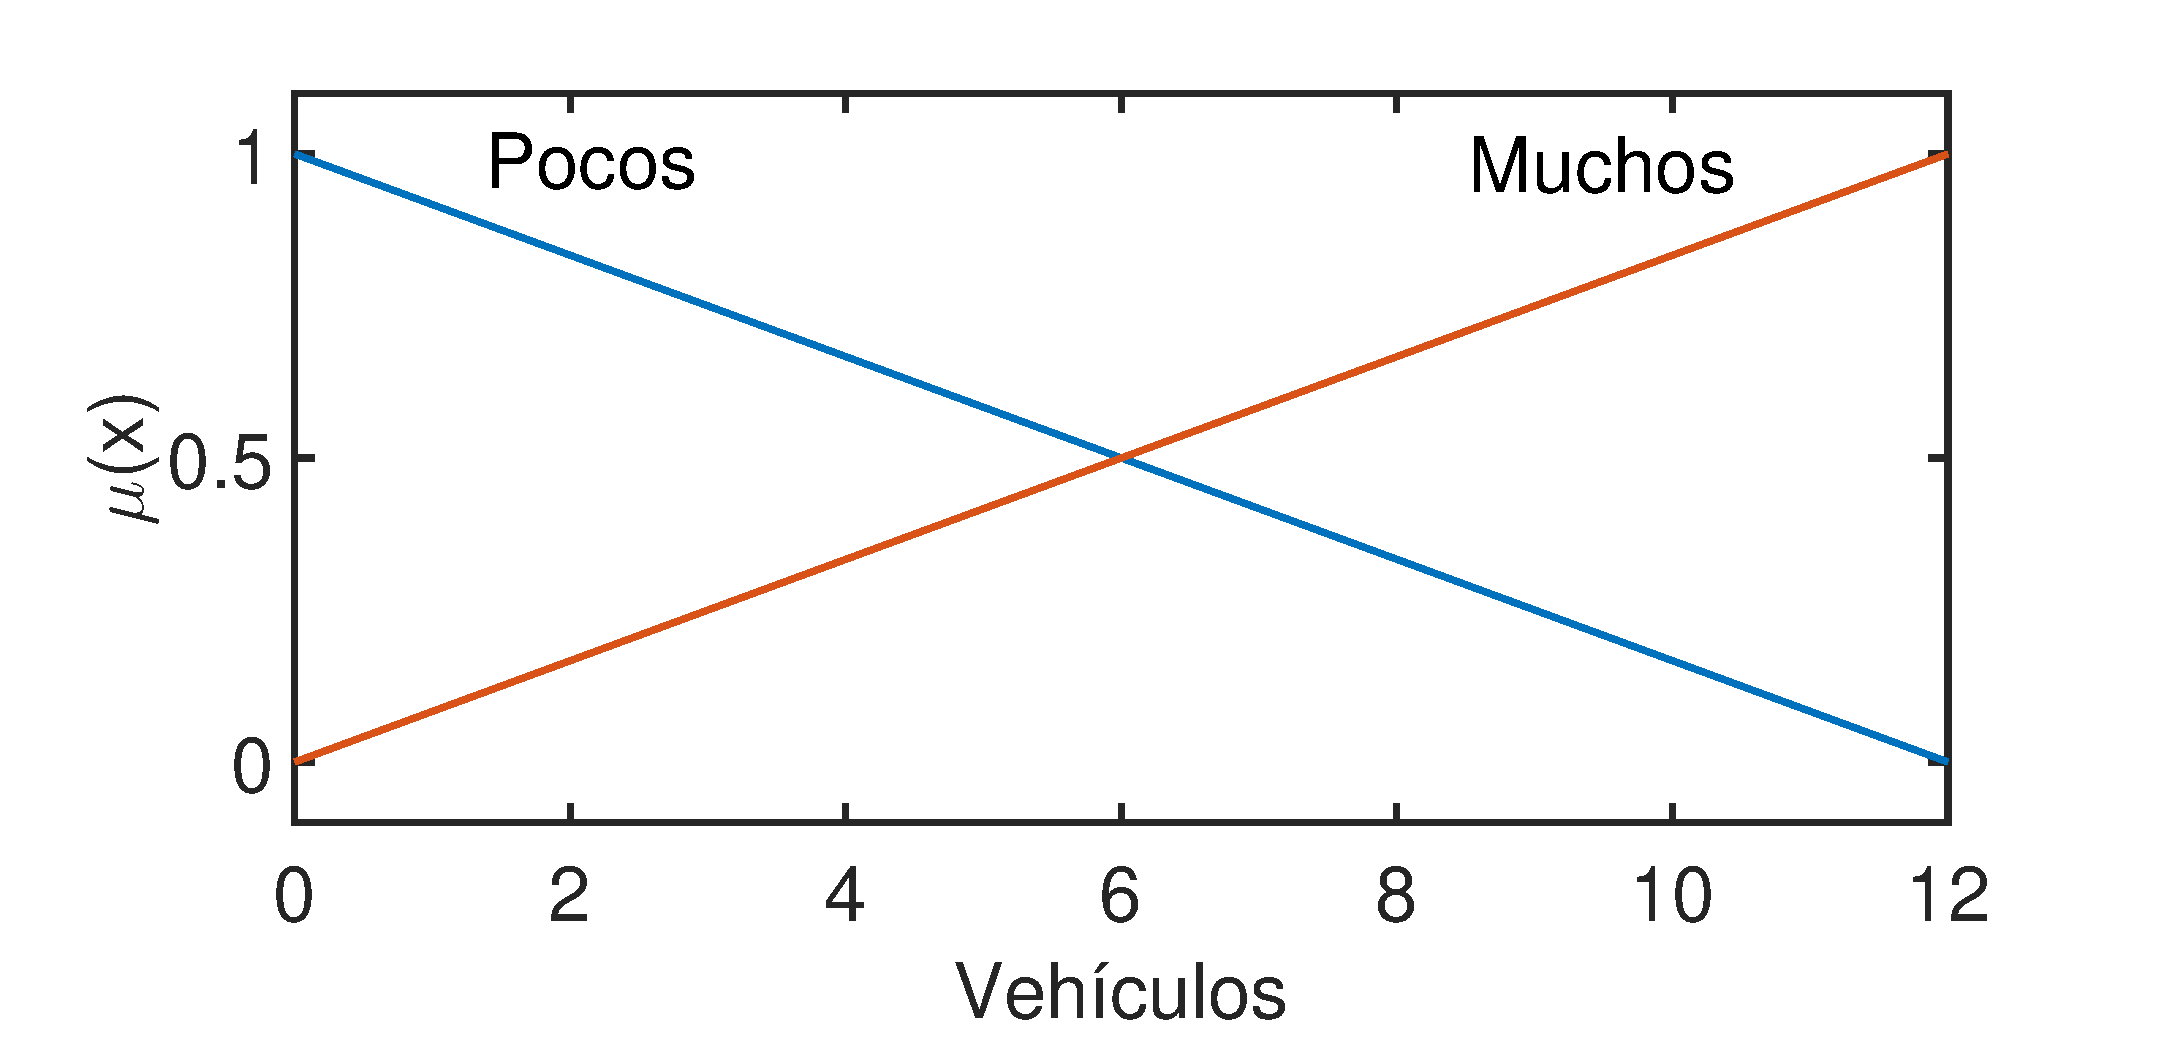
\includegraphics[height=4cm, width=8.1cm]{Variables/ConfigA_input1.eps}}
	\subfigure[Variable lingüística Congestión]{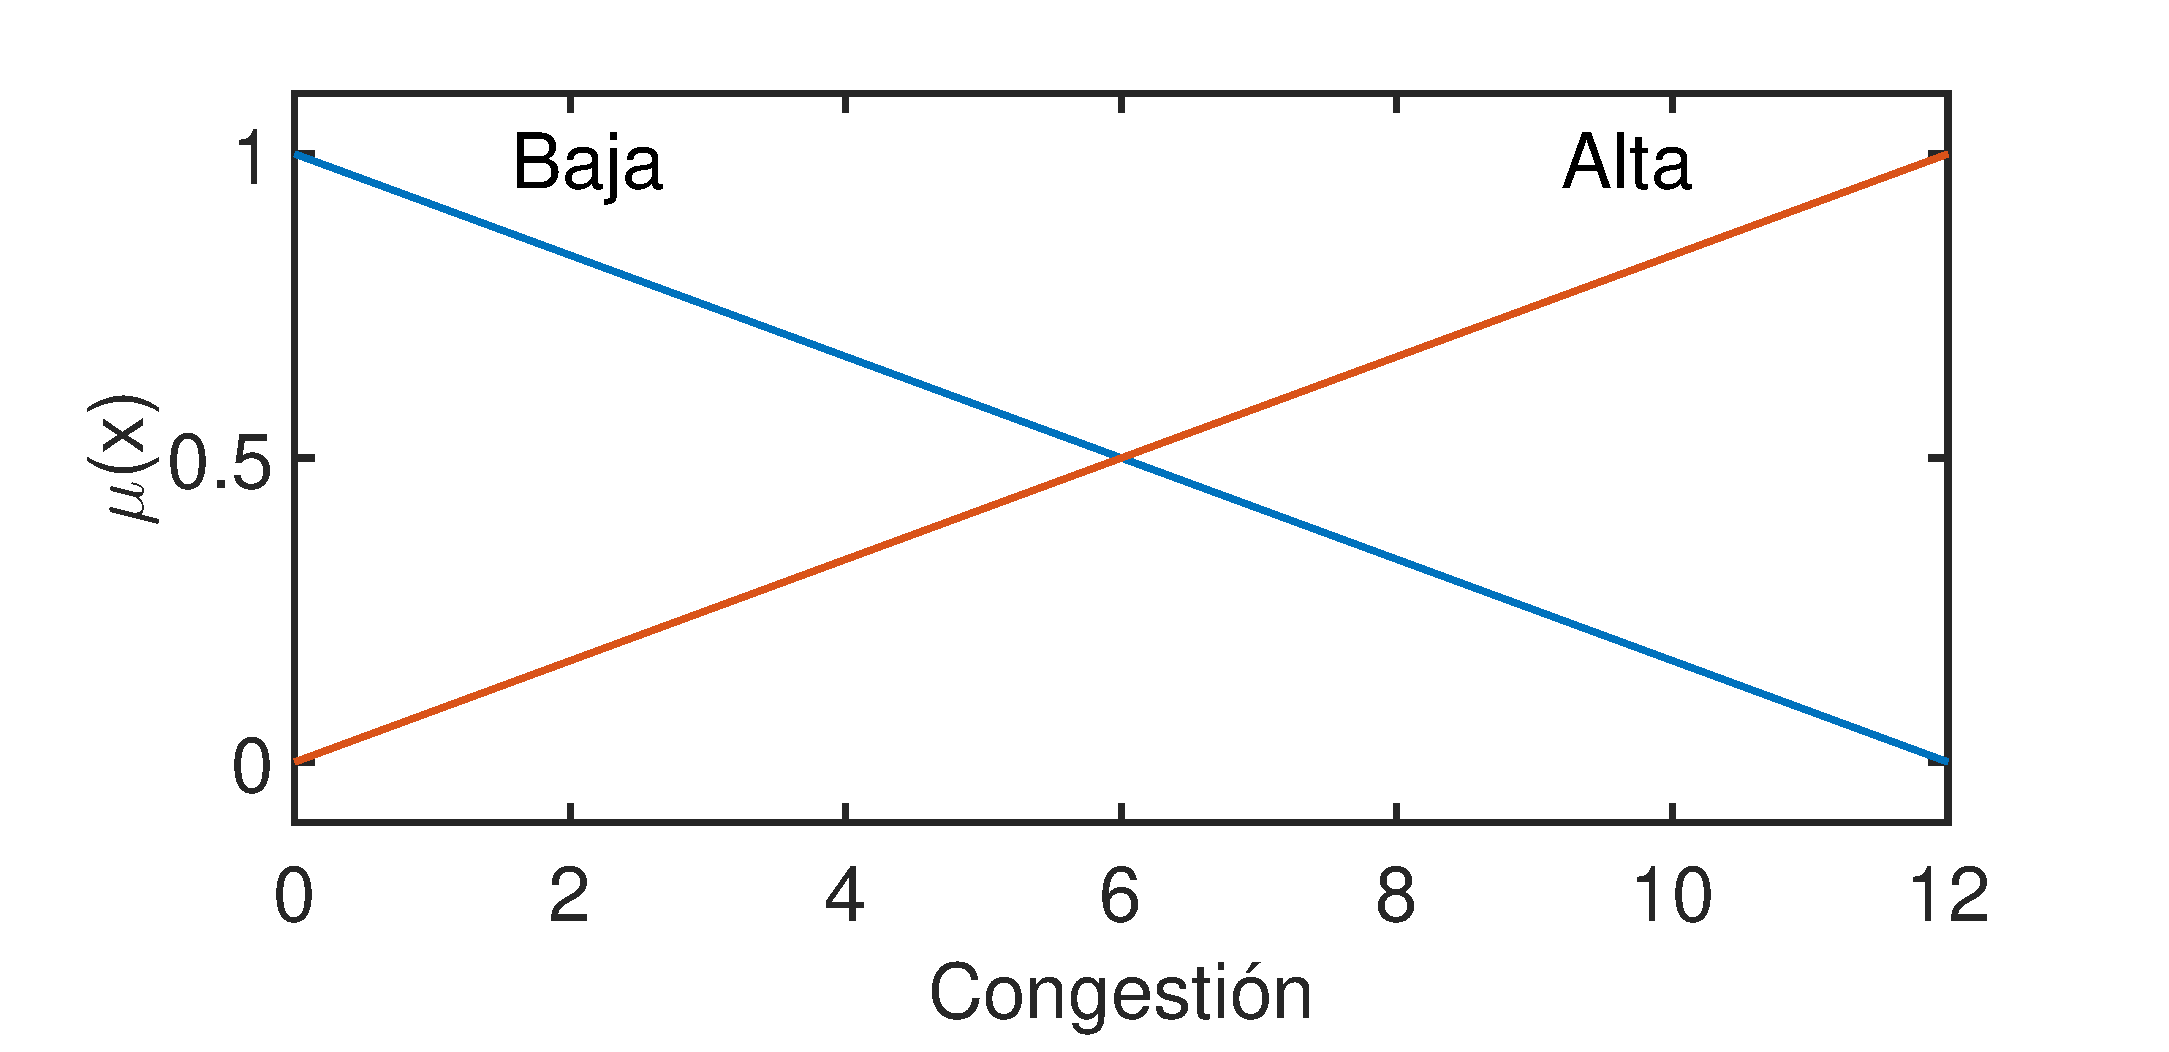
\includegraphics[height=4cm, width=8.1cm]{Variables/ConfigA_input2.eps}}
	\caption[Gráficas de las variables lingüísticas vehículos y congestión]{Representación gráfica de las variables lingüísticas Vehículos y Congestión }
\end{figure}

\newpage
\textbf{Variable de salida Tiempo.} Se refiere al tiempo en segundos que le será asignada a la fase verde actual. La variable se encuentra definida en un universo de discurso $U = [0,90]$.

\begin{table}[!h]
	\centering
	\begin{tabular}{llr} \toprule
		Termino lingüístico & Función de membresía & Parámetros \\ \midrule
		Bajo & Triangular & [0, 0, 30 ] \\
		Medio & Triangular & [0, 30, 60] \\
		Moderado & Triangular & [30, 60, 90] \\
		Alto & Triangular & [60, 90, 90] \\ \bottomrule
	\end{tabular}
	\caption{Variable lingüística \textit{Tiempo}}
\end{table}

\begin{figure}[H]
	\centering
	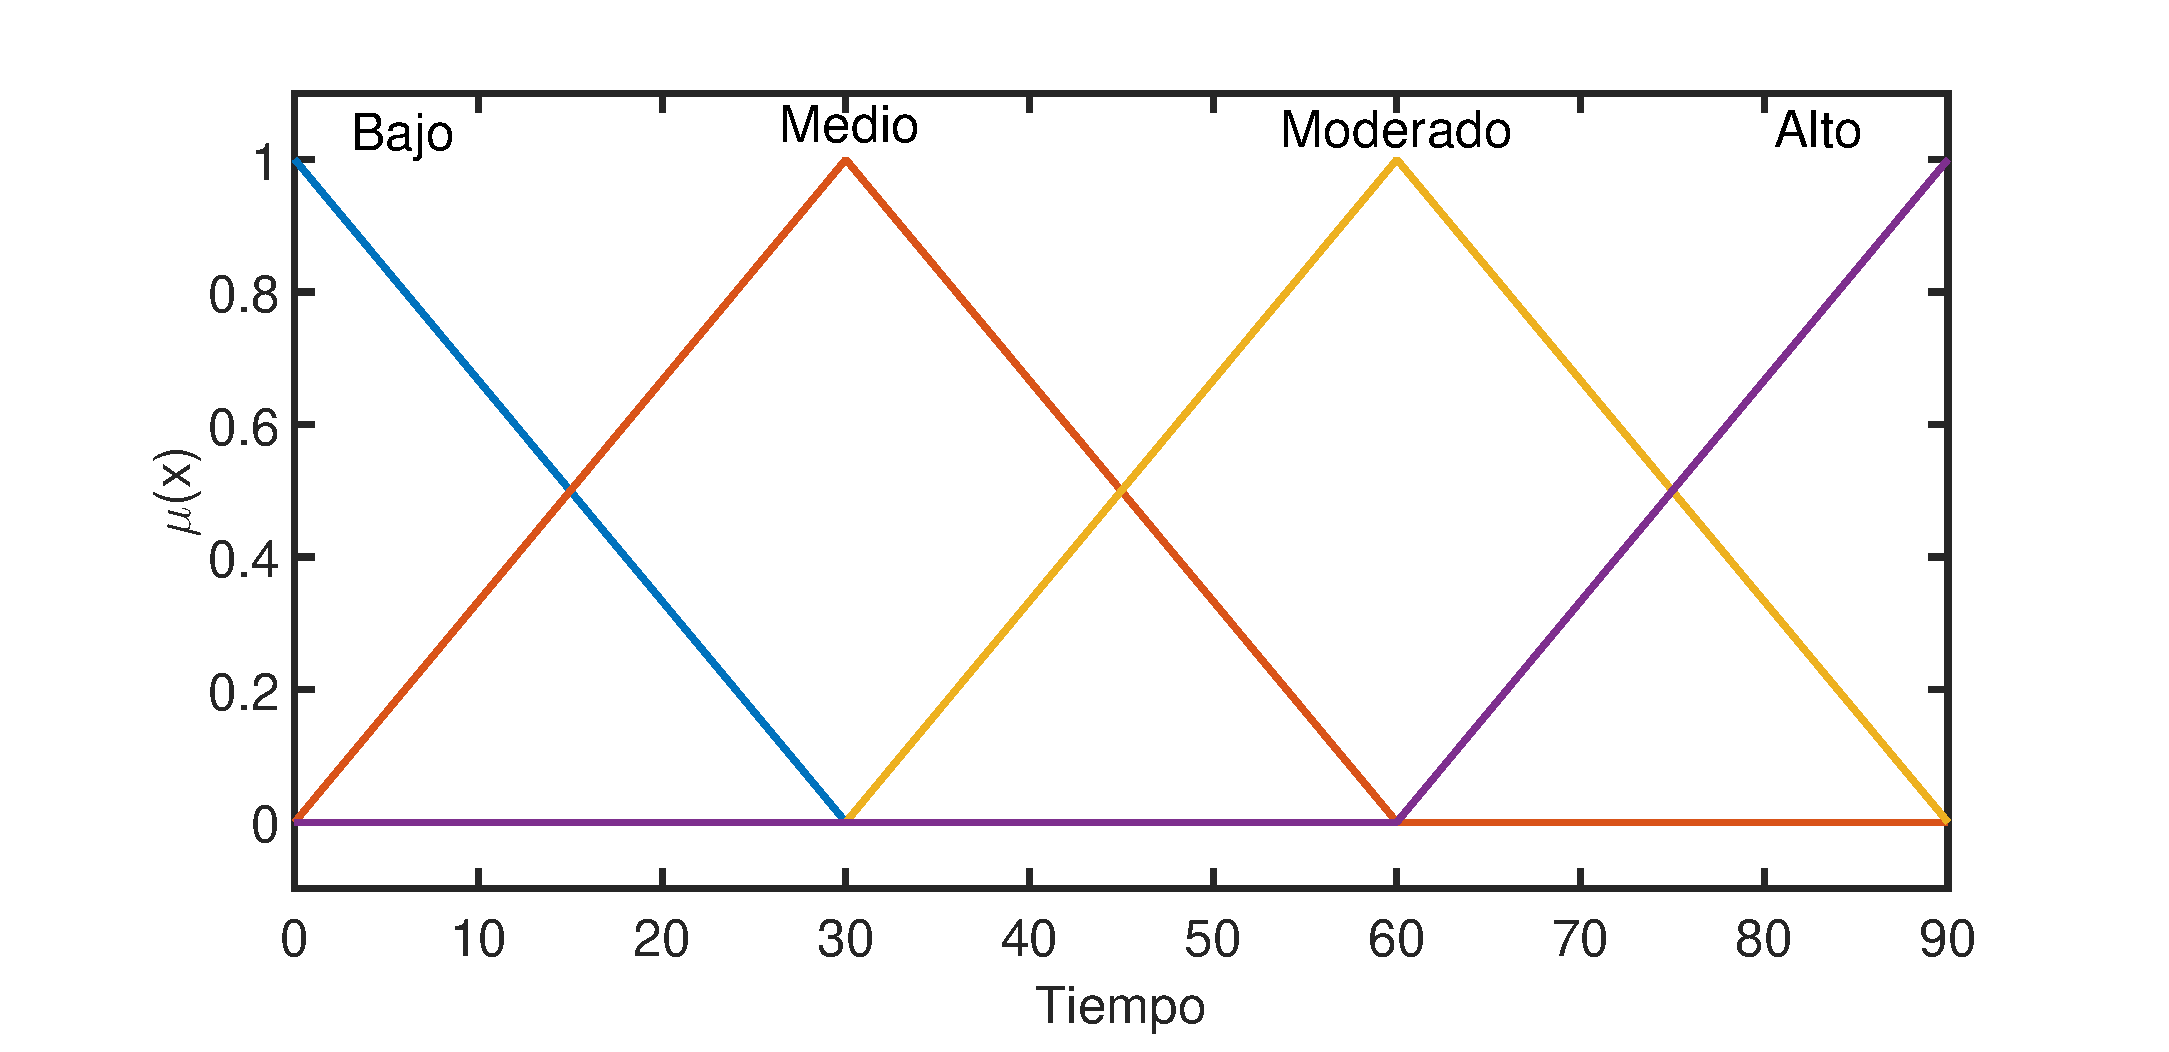
\includegraphics[height=5cm, width=12cm]{Variables/ConfigA_output1.eps}
	\caption[Gráfica variable lingüística tiempo - A]{Representación gráfica de la variable lingüística Tiempo}
\end{figure}

\subsubsection{Base de conocimientos}
El siguiente cuadro muestra las reglas difusas empleadas en esta configuración.
\begin{longtable}[c]{lclcl} \toprule
	\multicolumn{3}{c}{Antecedente} & & Consecuente \\ \midrule
	Vehículos Pocos & Y & Congestión Baja& $\rightarrow$ & Verde Medio \\
	Vehículos Pocos & Y & Congestión Alta& $\rightarrow$ & Verde Bajo \\
	Vehículos Muchos &Y& Congestión Baja& $\rightarrow$ & Verde Alto \\
	Vehículos Muchos &Y& Congestión Alta& $\rightarrow$ & Verde Moderado \\ \hline
	\caption{Reglas difusas para la configuración \textit{A}}
\end{longtable}

\newpage
\subsubsection{Resultados}


Una vez diseñado e implementado el sistema de inferencia, se le suministraron valores de prueba para evaluar su desempeño. Los resultados de dicha evaluación se reflejan en el cuadro siguiente:

\begin{table}[H]
	\centering
	\begin{tabular}{cccccc} \toprule
		$V \backslash C$ &  0 & 3 & 6 & 9 & 12 \\ \midrule
		0 & 30.00 & 28.99 & 26.21 & 20.86 & 09.70 \\
		3 & 39.02 & 39.03 & 37.69 & 35.58 & 33.96 \\
		6 & 46.40 & 45.83 & 45.00 & 44.16 & 43.59 \\
		9 & 56.03 & 54.41 & 52.30 & 50.96 & 50.97 \\
		12& 80.29 & 69.13 & 63.79 & 61.00 & 59.99 \\
		%\caption{Resultados de la evaluación para la configuración \textit{A}}
	\end{tabular}
	\caption{Resultados de la evaluación para la configuración}
\end{table}
Donde: la columna V son los valores de prueba de la variable Vehículos, la fila C son los valores de  prueba de la variable Congestión y las celdas son los tiempos (en segundos).




\subsubsection{Observaciones}
\begin{multicols}{2}

Después de evaluar el desempeño de la primera configuración se observa como efectivamente el tiempo asignado varía de acuerdo a las variables de entrada; sin embargo, el tiempo asignado para las entradas Vehículos = 0 y Congestión = 6, resulta excesivo puesto que la cantidad de vehículos a los que se les cederá el paso es mínimo (0) mientras que el índice de vehículos (6) que se mantendrán a la espera es bastante considerable.

\begin{figure}[H]
	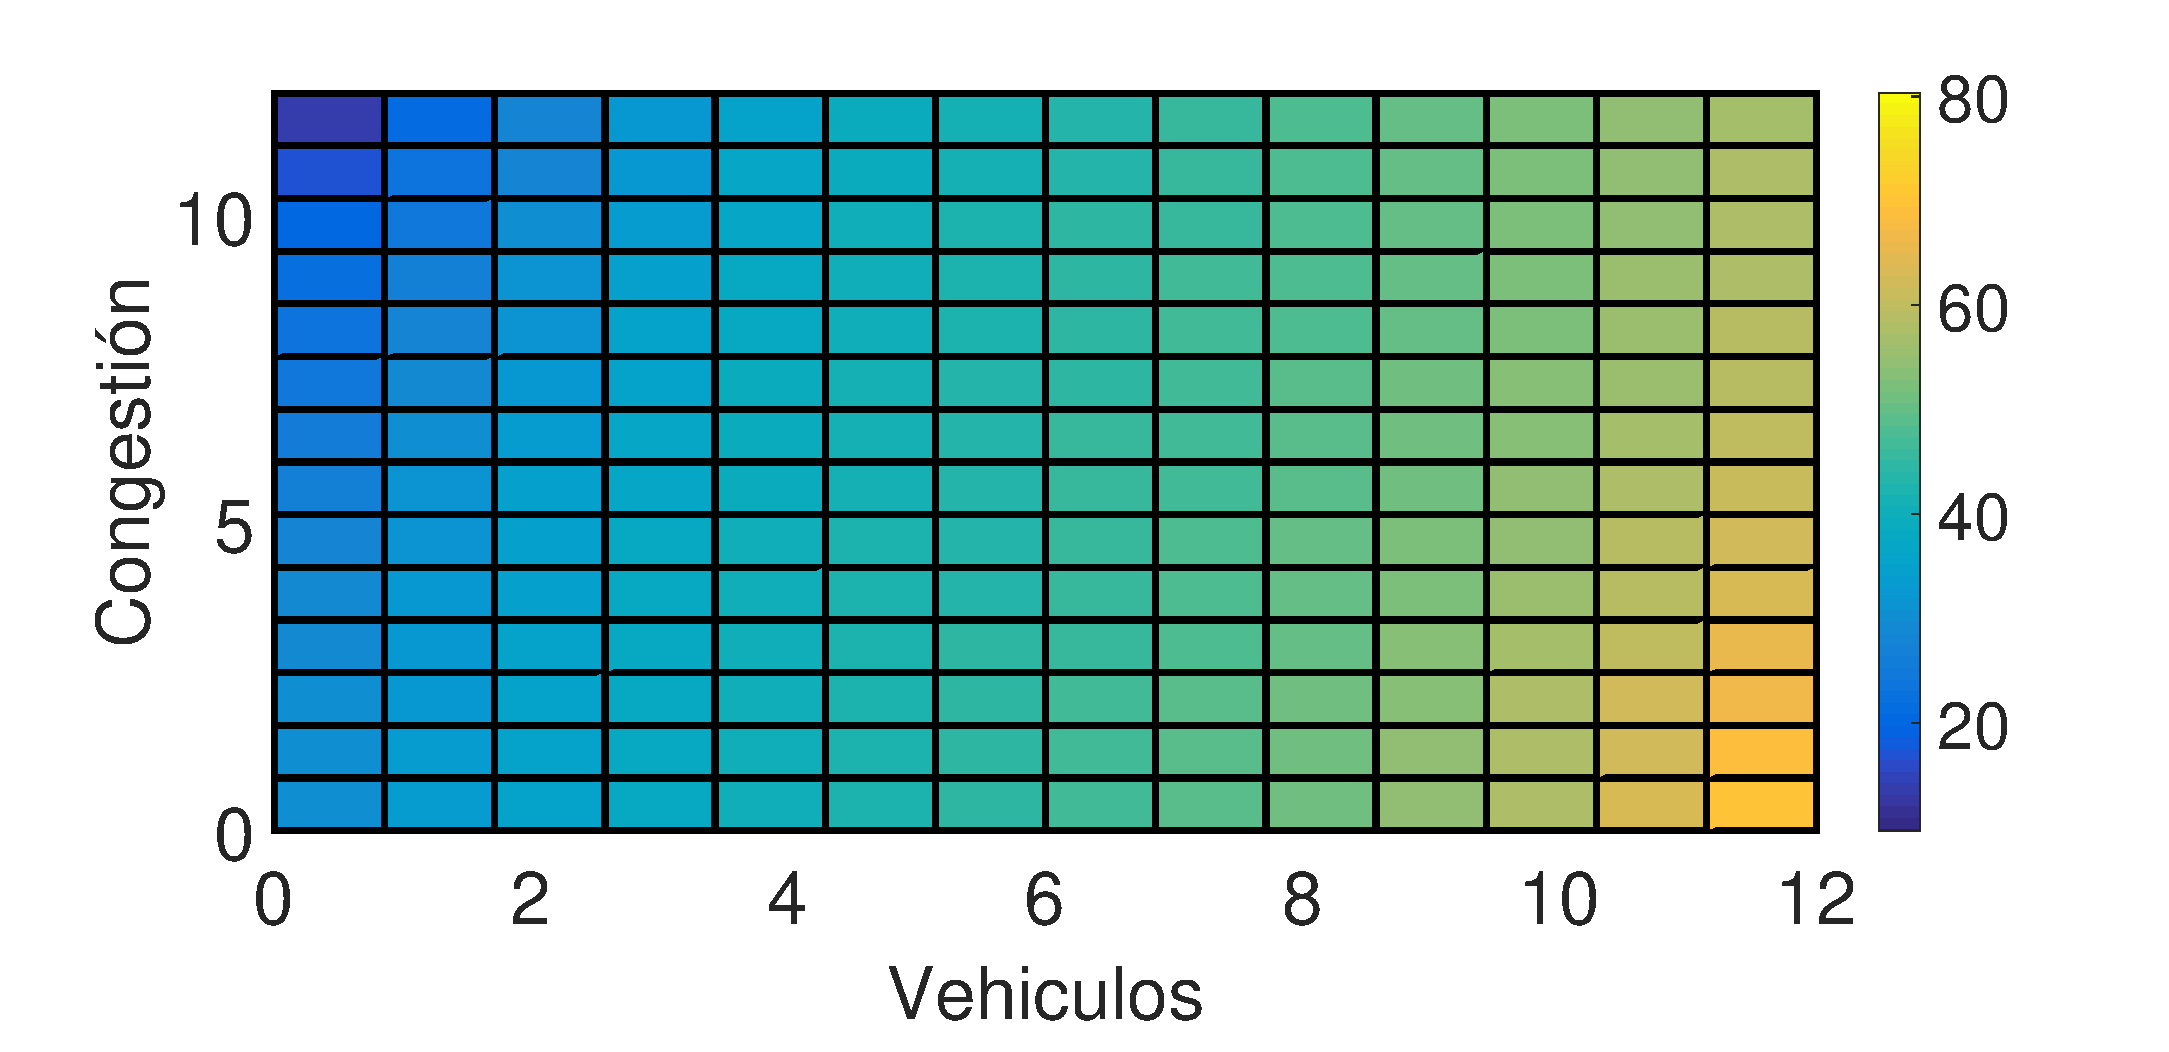
\includegraphics[width=0.5\textwidth]{Surfaces/Surface2D_A.eps}
	\caption{Superficie de control}
\end{figure}

\end{multicols}

 


\pagebreak
\subsection{Configuración B}
La configuración presentada en esta sección, ajusta los parámetros de las funciones de membresía de la variable de salida Tiempo. La configuración pasa a ser la siguiente: 

\textbf{Variable de entrada Vehículos.} Se mantiene sin cambios.

\begin{table}[!h]
	\centering
	\begin{tabular}{llr} \toprule
		Termino lingüístico & Función de membresía & Parámetros \\ \midrule
		Pocos & Triangular & [0, 0, 12 ] \\
		Muchos & Triangular & [0, 12, 12] \\ \bottomrule
	\end{tabular}
	\caption{Variable lingüística \textit{Vehículos}}
\end{table}


\textbf{Variable de entrada Congestión.} Se mantiene sin cambios desde la configuración anterior.


\begin{table}[!h]
	\centering
	\begin{tabular}{llr} \toprule
		Termino lingüístico & Función de membresía & Parámetros \\ \midrule
		Baja & Triangular & [0, 0, 12 ] \\
		Alta & Triangular & [0, 12, 12] \\ \bottomrule
	\end{tabular}
	\caption{Variable lingüística \textit{Congestión}}
\end{table}

\begin{figure}[H]
	\centering
	\subfigure[Variable lingüística Vehículos]{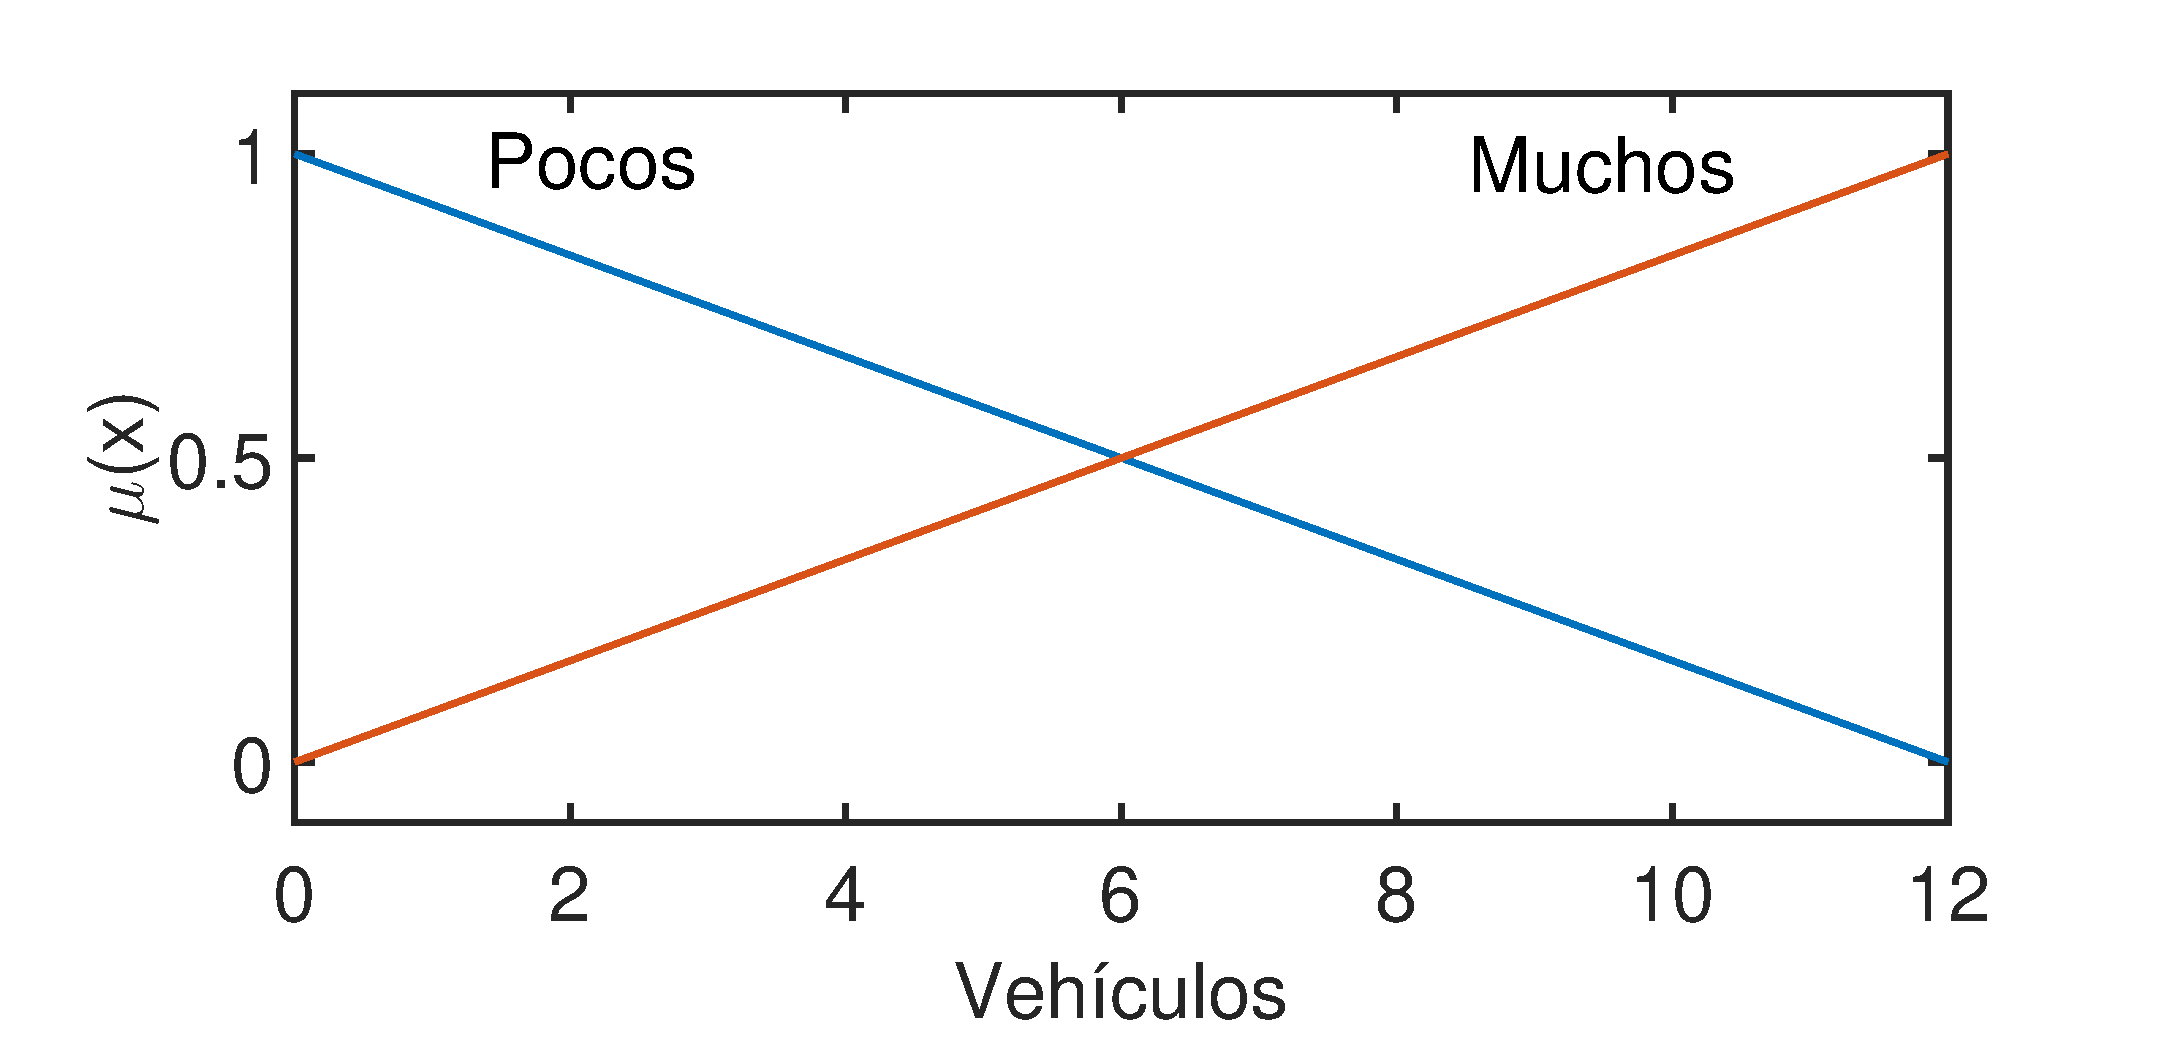
\includegraphics[height=4cm, width=8.1cm]{Variables/ConfigA_input1.eps}}
	\subfigure[Variable lingüística Congestión]{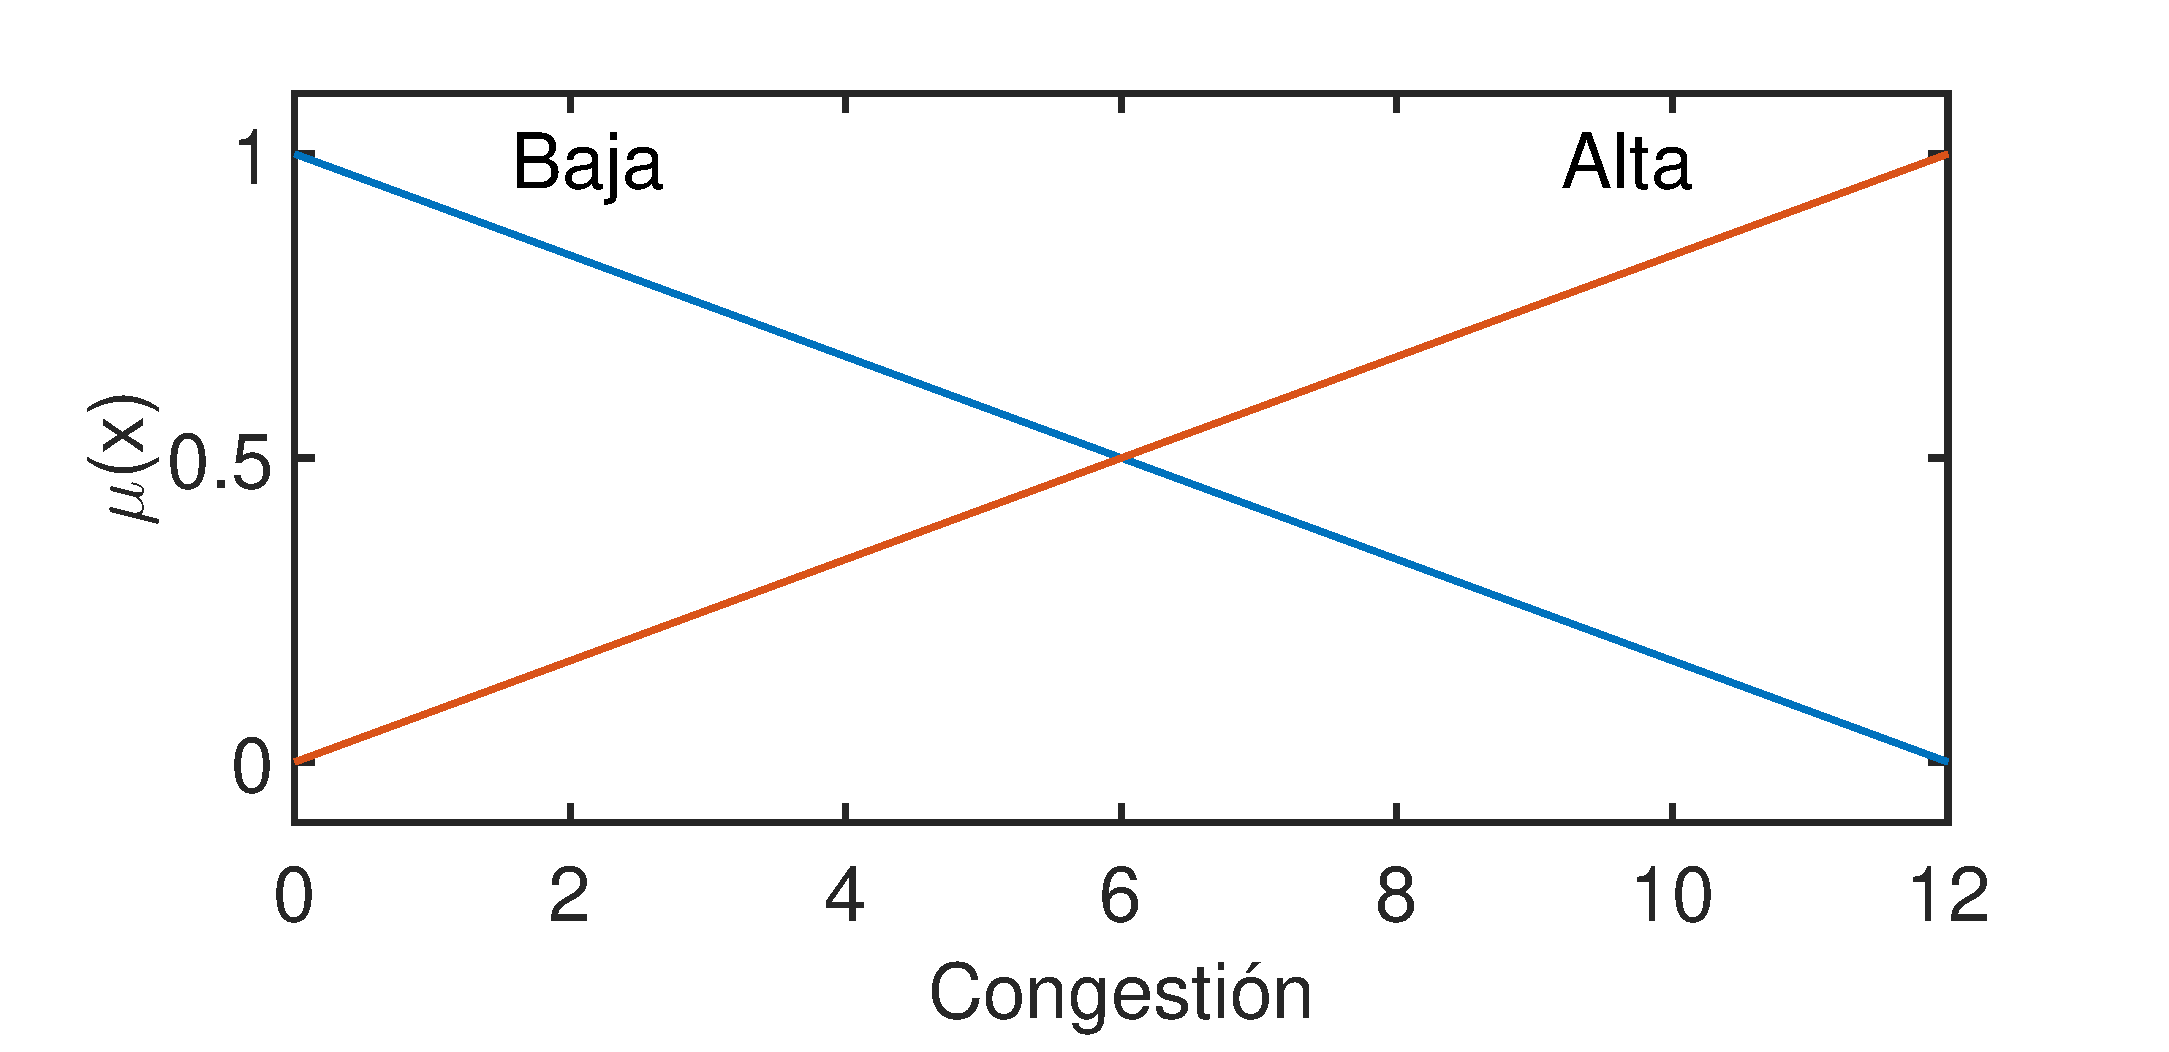
\includegraphics[height=4cm, width=8.1cm]{Variables/ConfigA_input2.eps}}
	\caption[Gráficas de las variables lingüísticas vehículos y congestión]{Representación gráfica de las variables lingüísticas Vehículos y Congestión }
\end{figure}

\pagebreak
\textbf{Variable de salida Tiempo.}
En esta ocasión los parámetros de las funciones de membresía fueron ajustados para generar tiempos más acertados. La nueva configuración de esta variable se muestra a continuación:


\begin{table}[!h]
	\centering
	\begin{tabular}{llr} \toprule
		Termino lingüístico & Función de membresía & Parámetros \\ \midrule
		Bajo & Triangular & [0, 0, 20 ] \\
		Medio & Triangular & [0, 20, 45] \\
		Moderado & Triangular & [20, 45, 70] \\
		Alto & Triangular & [45, 70, 70] \\ \bottomrule
	\end{tabular}
	\caption{Variable lingüística \textit{Tiempo}}
\end{table}

\begin{figure}[H]
	\centering
	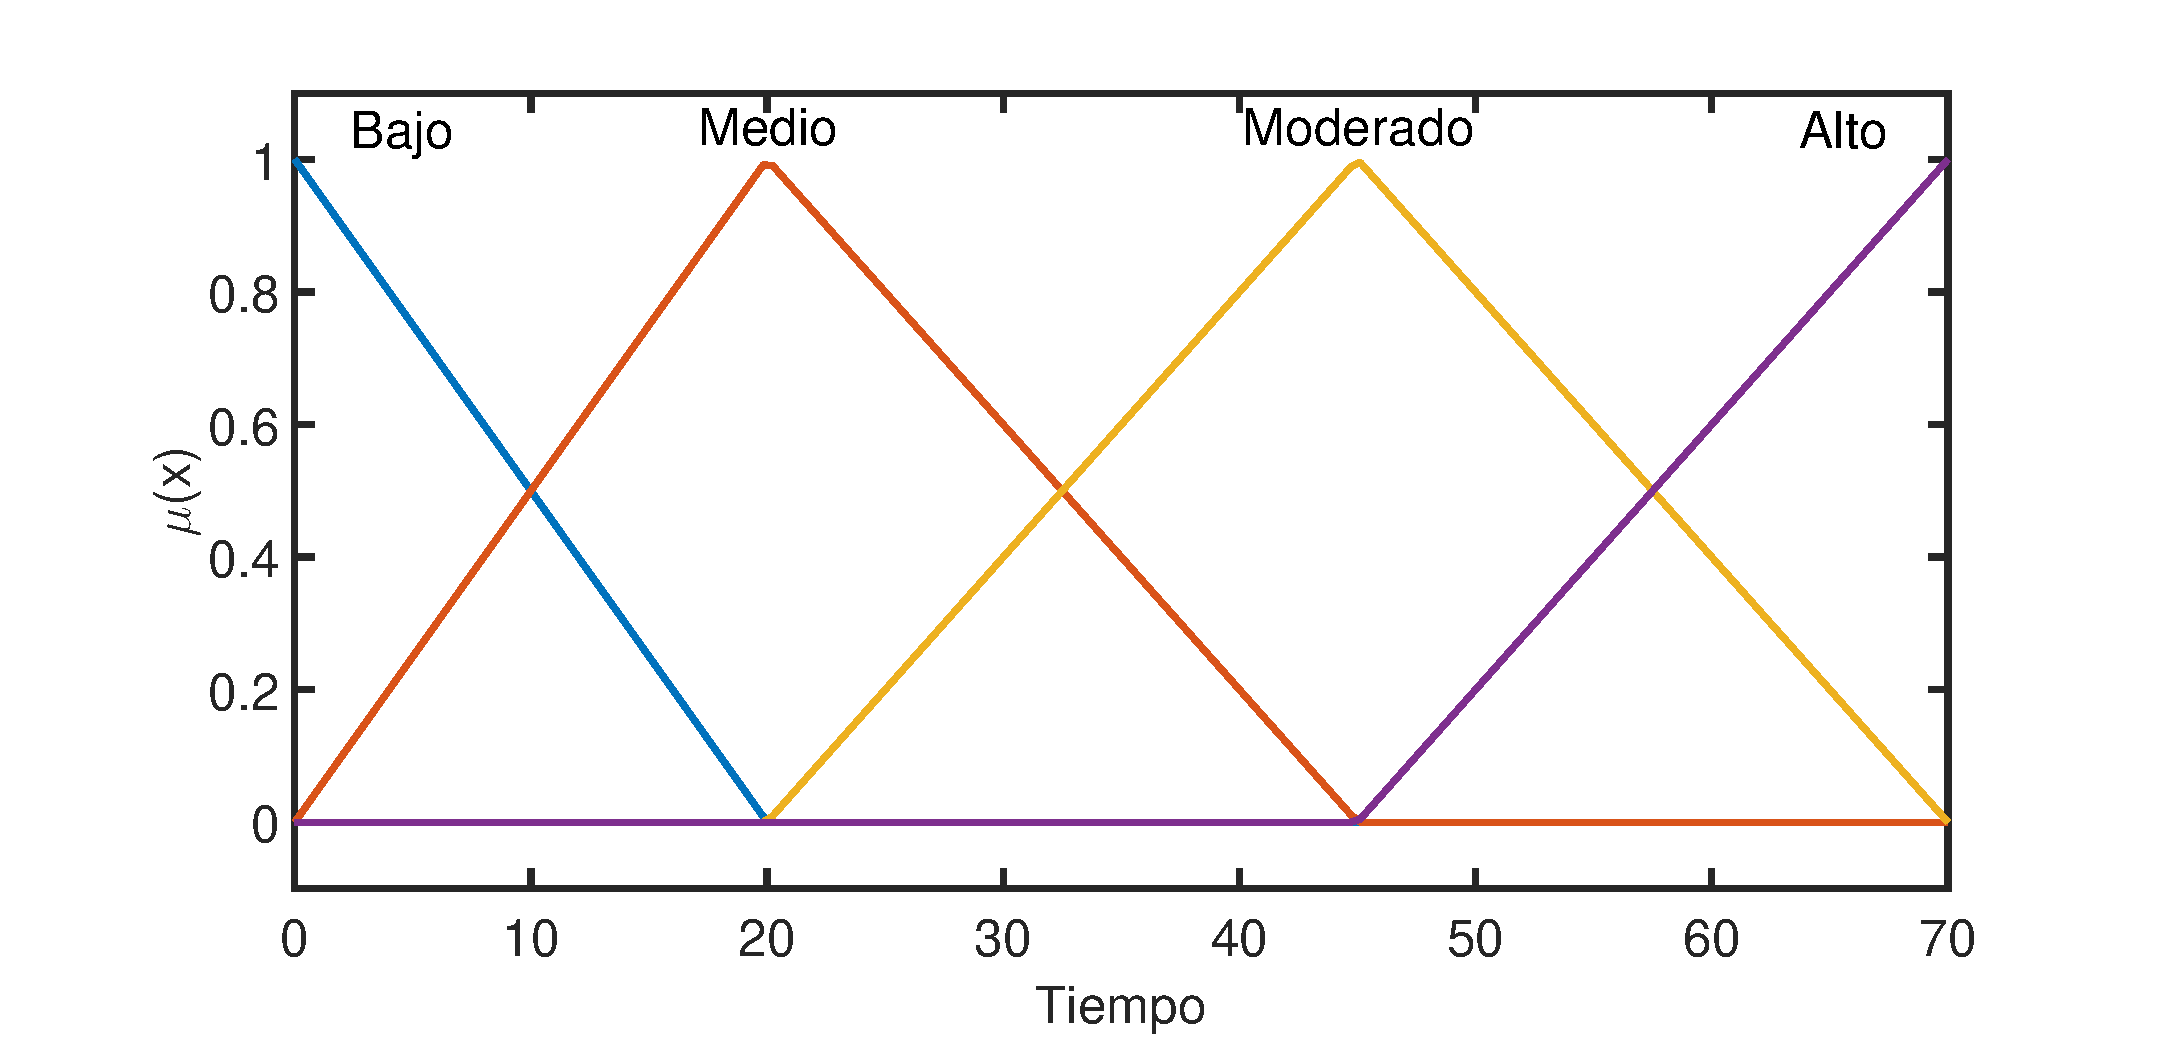
\includegraphics[height=5cm, width=12cm]{Variables/ConfigB_output1.eps}
	\caption[Gráfica variable lingüística tiempo - B]{Representación gráfica de la variable lingüística Tiempo}
\end{figure}

\subsubsection{Base de conocimientos}
El siguiente cuadro muestra las reglas difusas empleadas en esta configuración que se mantiene sin cambios.
\begin{longtable}[c]{lclcl} \toprule
	\multicolumn{3}{c}{Antecedente} & & Consecuente \\ \midrule
	Vehículos Pocos & Y & Congestión Baja& $\rightarrow$ & Verde Medio \\
	Vehículos Pocos & Y & Congestión Alta& $\rightarrow$ & Verde Bajo \\
	Vehículos Muchos &Y& Congestión Baja& $\rightarrow$ & Verde Alto \\
	Vehículos Muchos &Y& Congestión Alta& $\rightarrow$ & Verde Moderado \\ \hline
	\caption{Reglas difusas para la configuración \textit{B}}
\end{longtable}

\pagebreak
\subsubsection{Resultados}
Una vez reajustados los parámetros del sistema de inferencia, se le suministraron lo mismos valores de prueba para evaluar su desempeño respecto a la configuración anterior. Los resultados de dicha evaluación se reflejan en el cuadro siguiente:

\begin{longtable}[c]{cccccc} \toprule
	$V \backslash C$ &  0 & 3 & 6 & 9 & 12 \\ \midrule
	0 & 21.67 & 21.09 & 19.37 & 15.68 & 06.44 \\
	3 & 29.56 & 29.69 & 29.16 & 28.26 & 27.11 \\
	6 & 35.87 & 35.51 & 35.00 & 34.49 & 34.13 \\
	9 & 43.75 & 42.58 & 40.44 & 39.14 & 39.18 \\
	12& 61.90 & 52.60 & 48.15 & 45.83 & 45.00 \\
	\caption{Resultados de la evaluación para la configuración \textit{B}}
\end{longtable}

Donde: la columna V son los valores de prueba de la variable Vehículos, la fila C son los valores de  prueba de la variable Congestión y las celdas son los tiempos (en segundos) obtenidos por la configuración actual.

\subsubsection{Observaciones}
\begin{multicols}{2}
Después de evaluar el desempeño de la segunda configuración se observa como efectivamente el tiempo asignado es más acorde a la cantidad de vehículos; sin embargo, el tiempo asignado para las entradas Vehículos = 0 y Congestión = 0, resulta generoso puesto que la cantidad de vehículos a los que se les cederá el paso es mínimo (0) mientras al igual que el índice de vehículos (6); Sería mejor que en estos casos el tiempo fuera más corto para acelerar el ciclo del semáforo y reducir la espera de las otras avenidas. En otro casos como V = 12 y C = 12, el tiempo podría resultar insuficiente para desahogar el tráfico, por lo que se ajustará en la siguiente configuración.

\begin{figure}[H]
	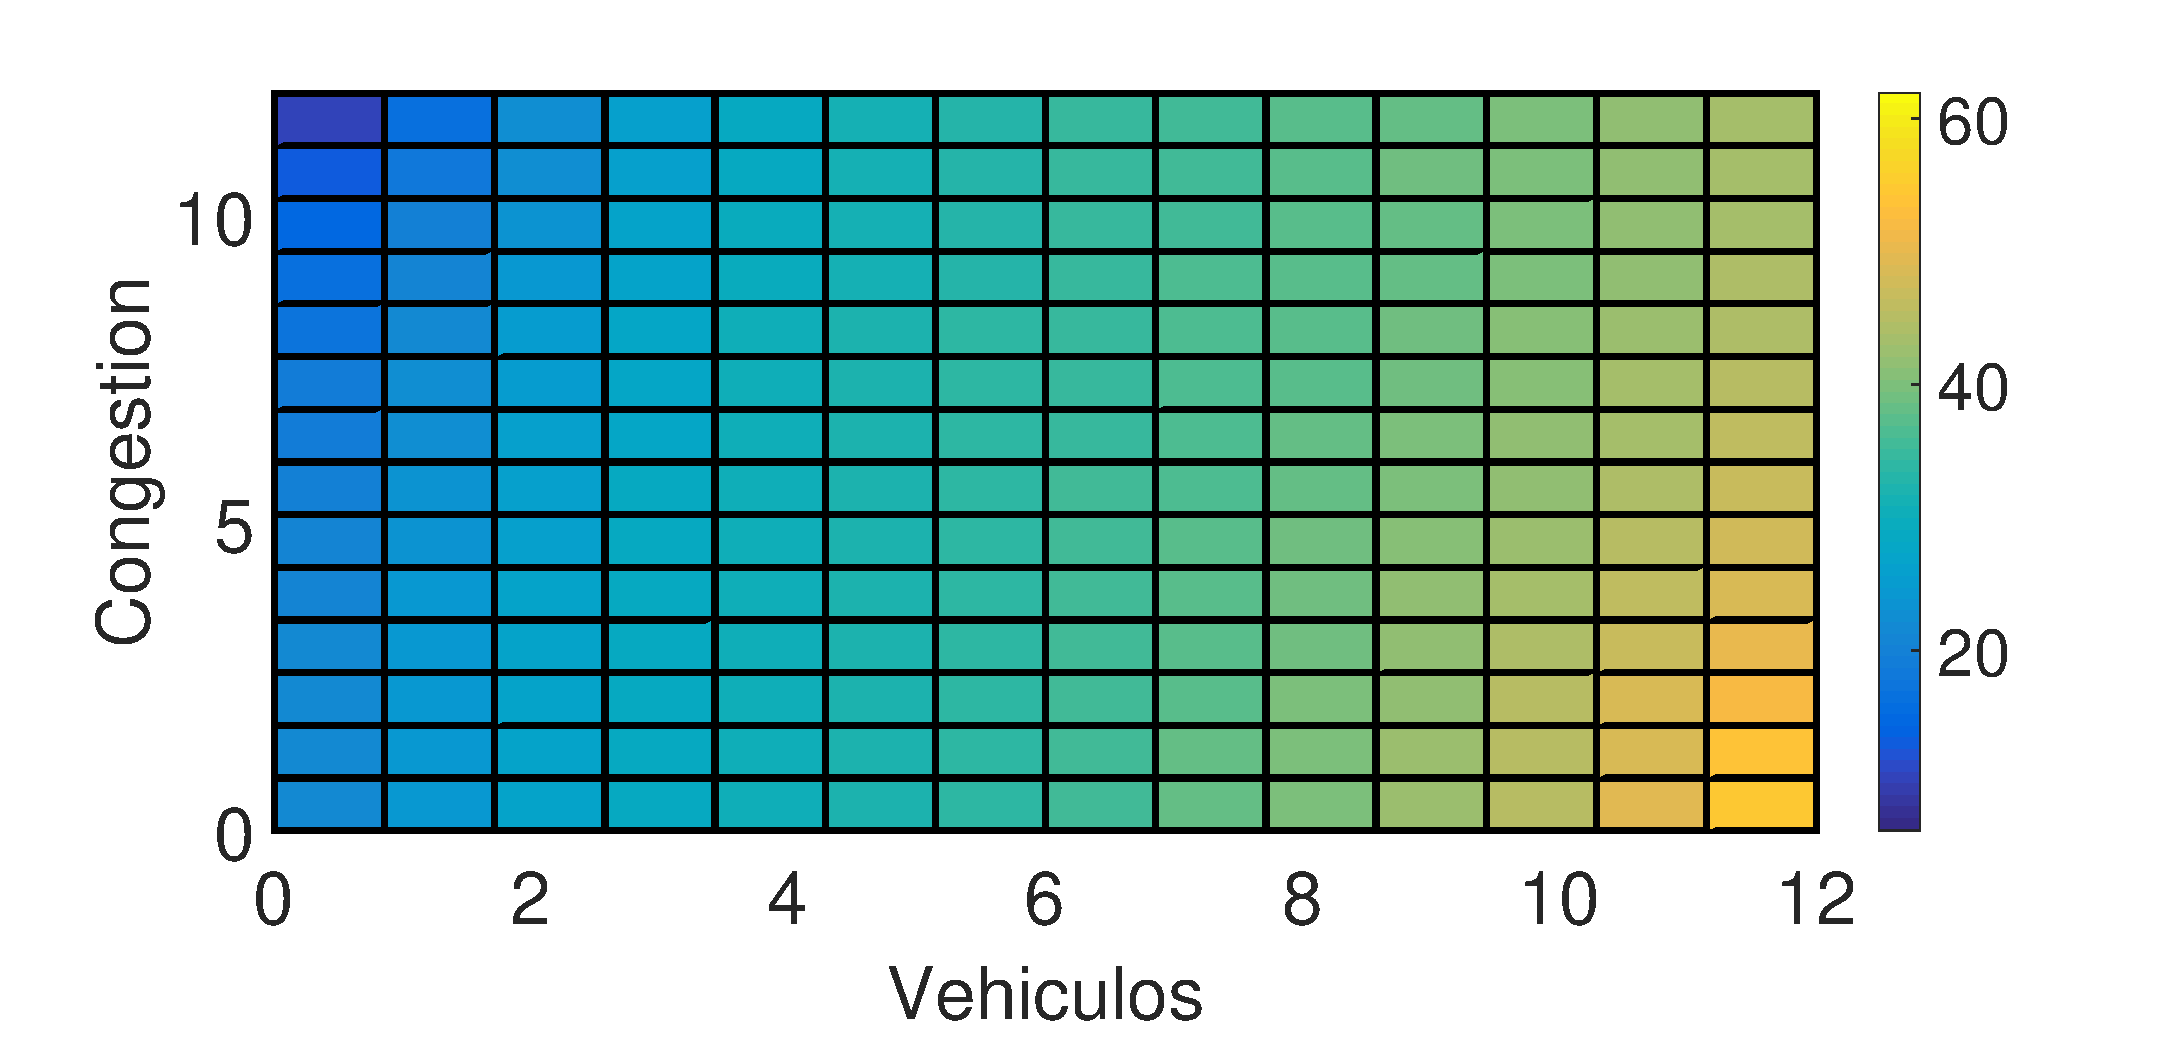
\includegraphics[width=0.5\textwidth]{Surfaces/Surface2D_B.eps}
	\caption{Superficie de control}
\end{figure}

\end{multicols}


\pagebreak
\subsection{Configuración C}
En está ocasión los reajustes serán mayores a los de la configuración anterior. Puesto que se agregaran un nuevo termino lingüístico a las variables Vehículos y Tiempo.

\textbf{Variable de entrada Vehículos.} Se agrega un nuevo término lingüístico para aumentar la flexibilidad del sistema.

\begin{table}[!h]
	\centering
	\begin{tabular}{llr} \toprule
		Termino lingüístico & Función de membresía & Parámetros \\ \midrule
		Pocos & Triangular & [0, 0, 6 ] \\
		Moderados & Triangular & [0, 6, 12 ] \\
		Muchos & Triangular & [6, 12, 12] \\ \bottomrule
	\end{tabular}
	\caption{Variable lingüística \textit{Vehículos}}
\end{table}


\textbf{Variable de entrada Congestión.} Se mantiene sin cambios desde la configuración anterior.


\begin{table}[!h]
	\centering
	\begin{tabular}{llr} \toprule
		Termino lingüístico & Función de membresía & Parámetros \\ \midrule
		Baja & Triangular & [0, 0, 12 ] \\
		Alta & Triangular & [0, 12, 12] \\ \bottomrule
	\end{tabular}
	\caption{Variable lingüística \textit{Congestión}}
\end{table}

\begin{figure}[H]
	\centering
	\subfigure[Variable lingüística Vehículos]{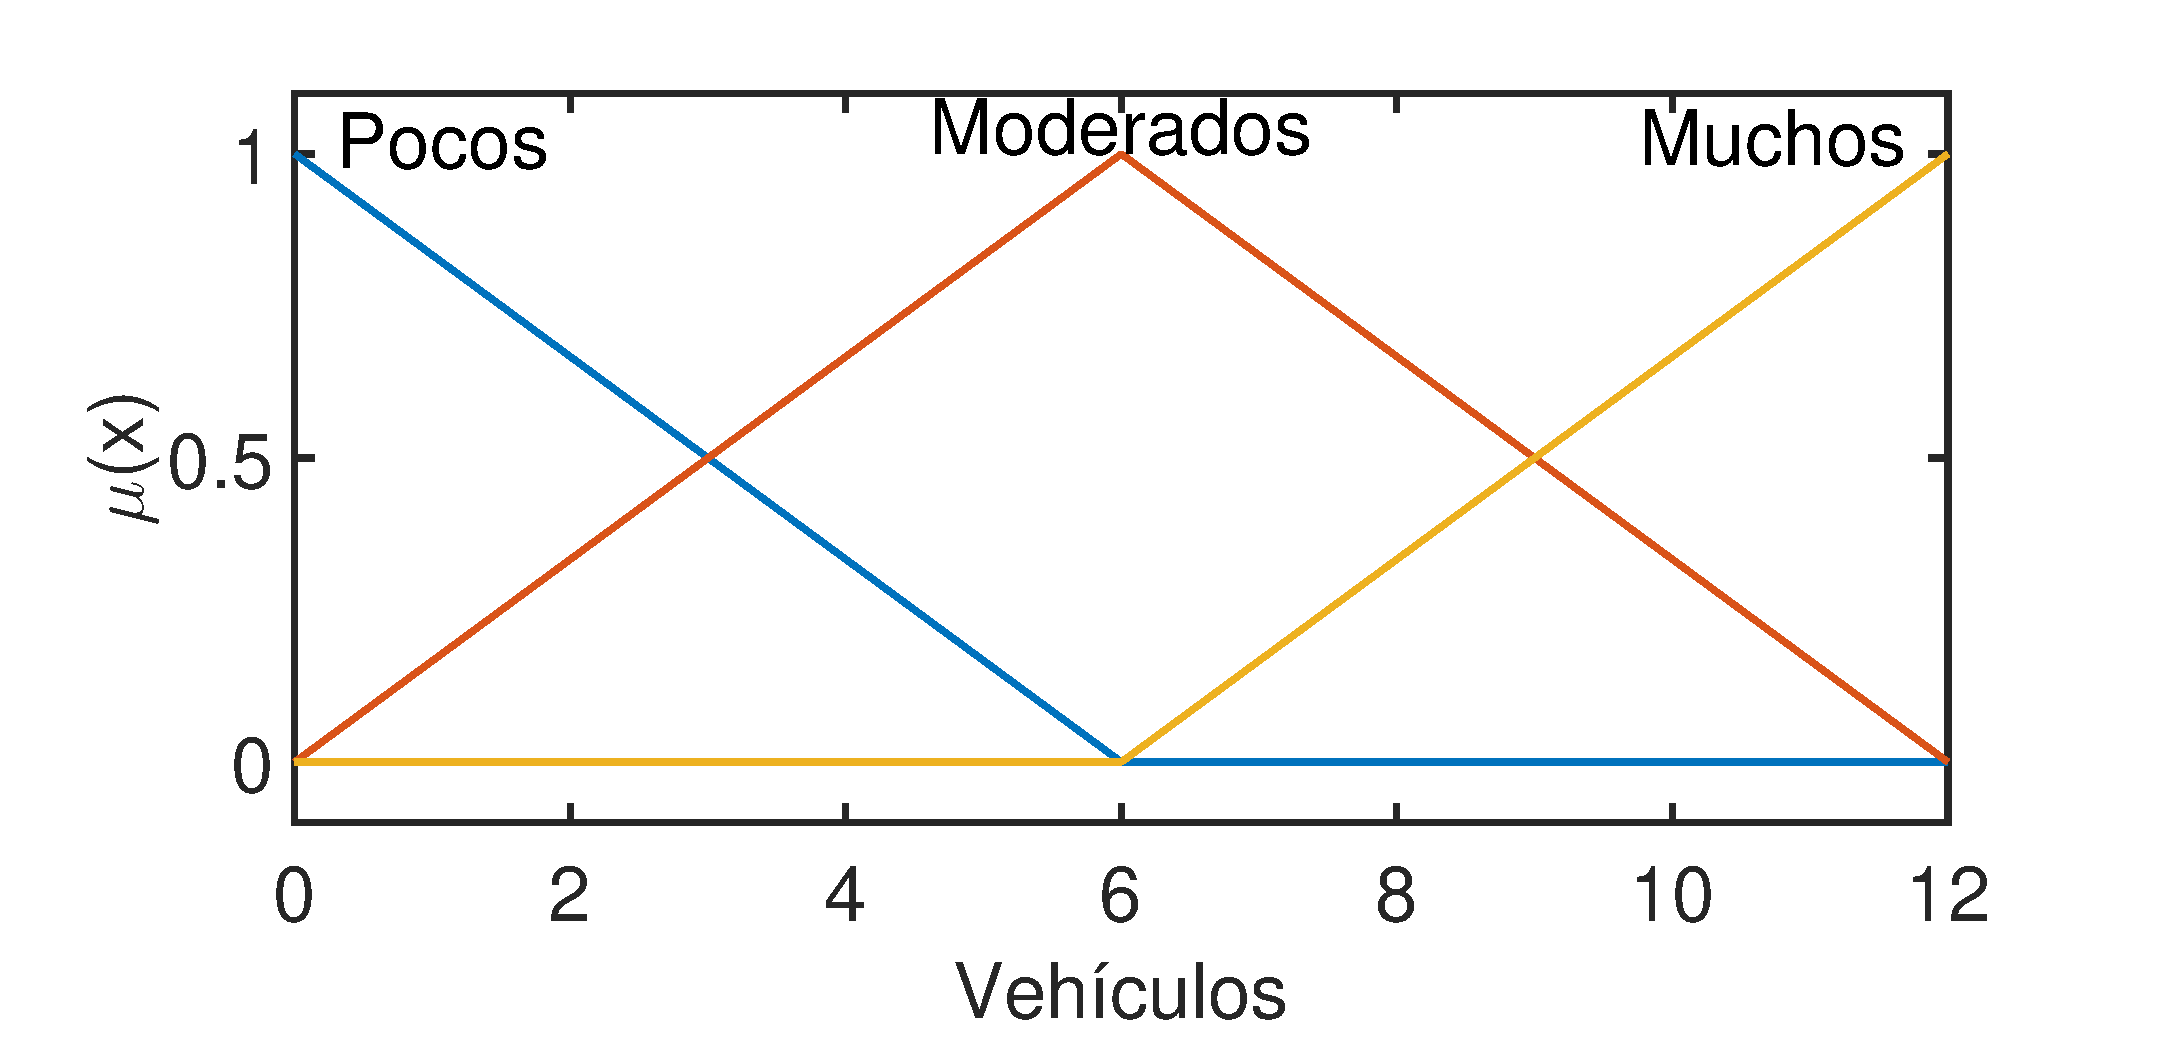
\includegraphics[height=4cm, width=8.1cm]{Variables/ConfigC_input1.eps}}
	\subfigure[Variable lingüística Congestión]{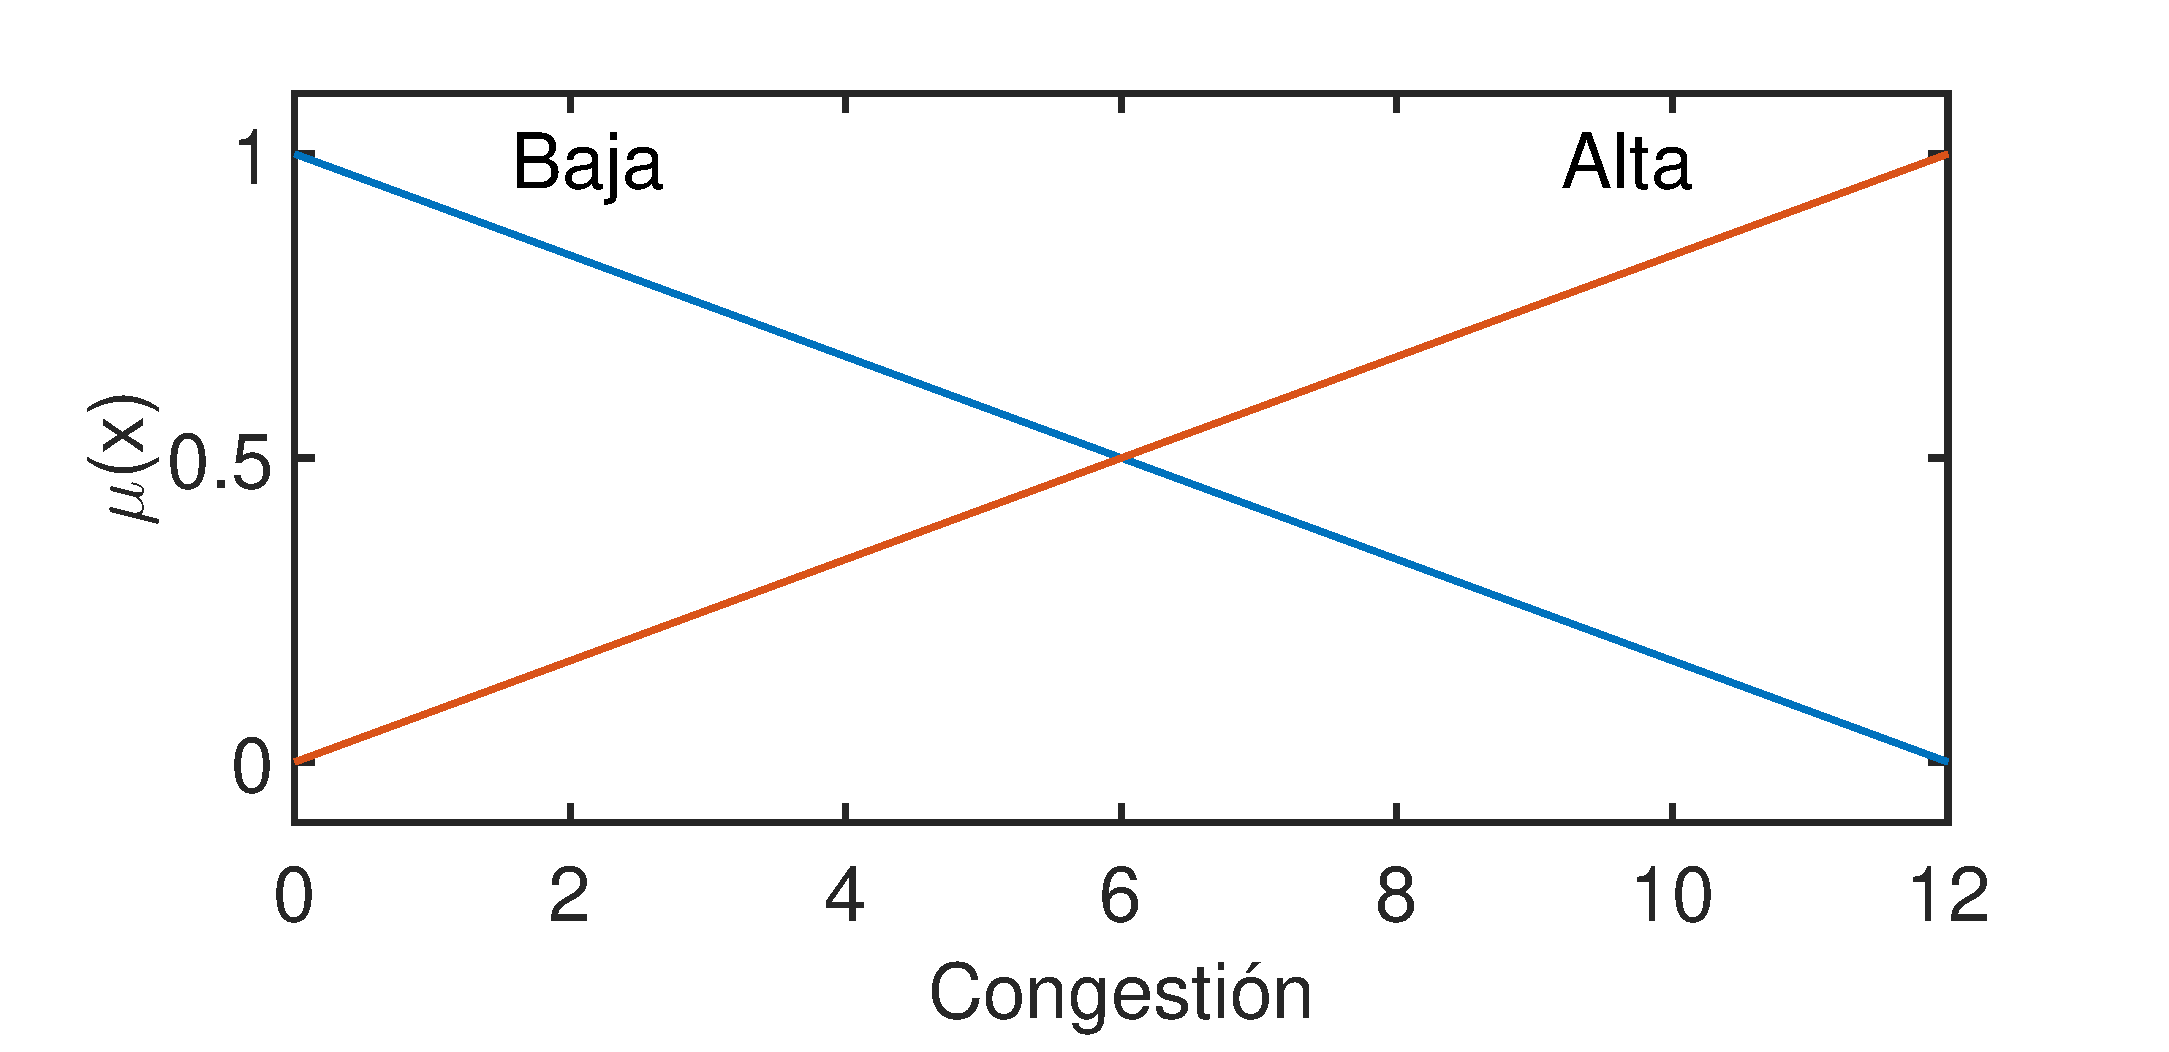
\includegraphics[height=4cm, width=8.1cm]{Variables/ConfigA_input2.eps}}
	\caption[Gráficas de las variables lingüísticas vehículos y congestión]{Representación gráfica de las variables lingüísticas Vehículos y Congestión }
\end{figure}

\pagebreak
\textbf{Variable de salida Tiempo.} Al igual que la variable vehículos, se ha agregado un nuevo término lingüístico para aumentar la flexibilidad. Además los parámetros de las funciones fueron reajustados ligeramente al igual que sus etiquetas.

\begin{table}[!h]
	\centering
	\begin{tabular}{llr} \toprule
		Termino lingüístico & Función de membresía & Parámetros \\ \midrule
		Mínimo & Triangular & [0, 10, 20 ] \\
		Bajo & Triangular & [0, 20, 40 ] \\
		Medio & Triangular & [20, 40, 60] \\
		Alto & Triangular & [40, 60, 80] \\
		Extra & Triangular & [60, 80, 80] \\ \bottomrule
	\end{tabular}
	\caption{Variable lingüística \textit{Tiempo}}
\end{table}

\begin{figure}[H]
	\centering
	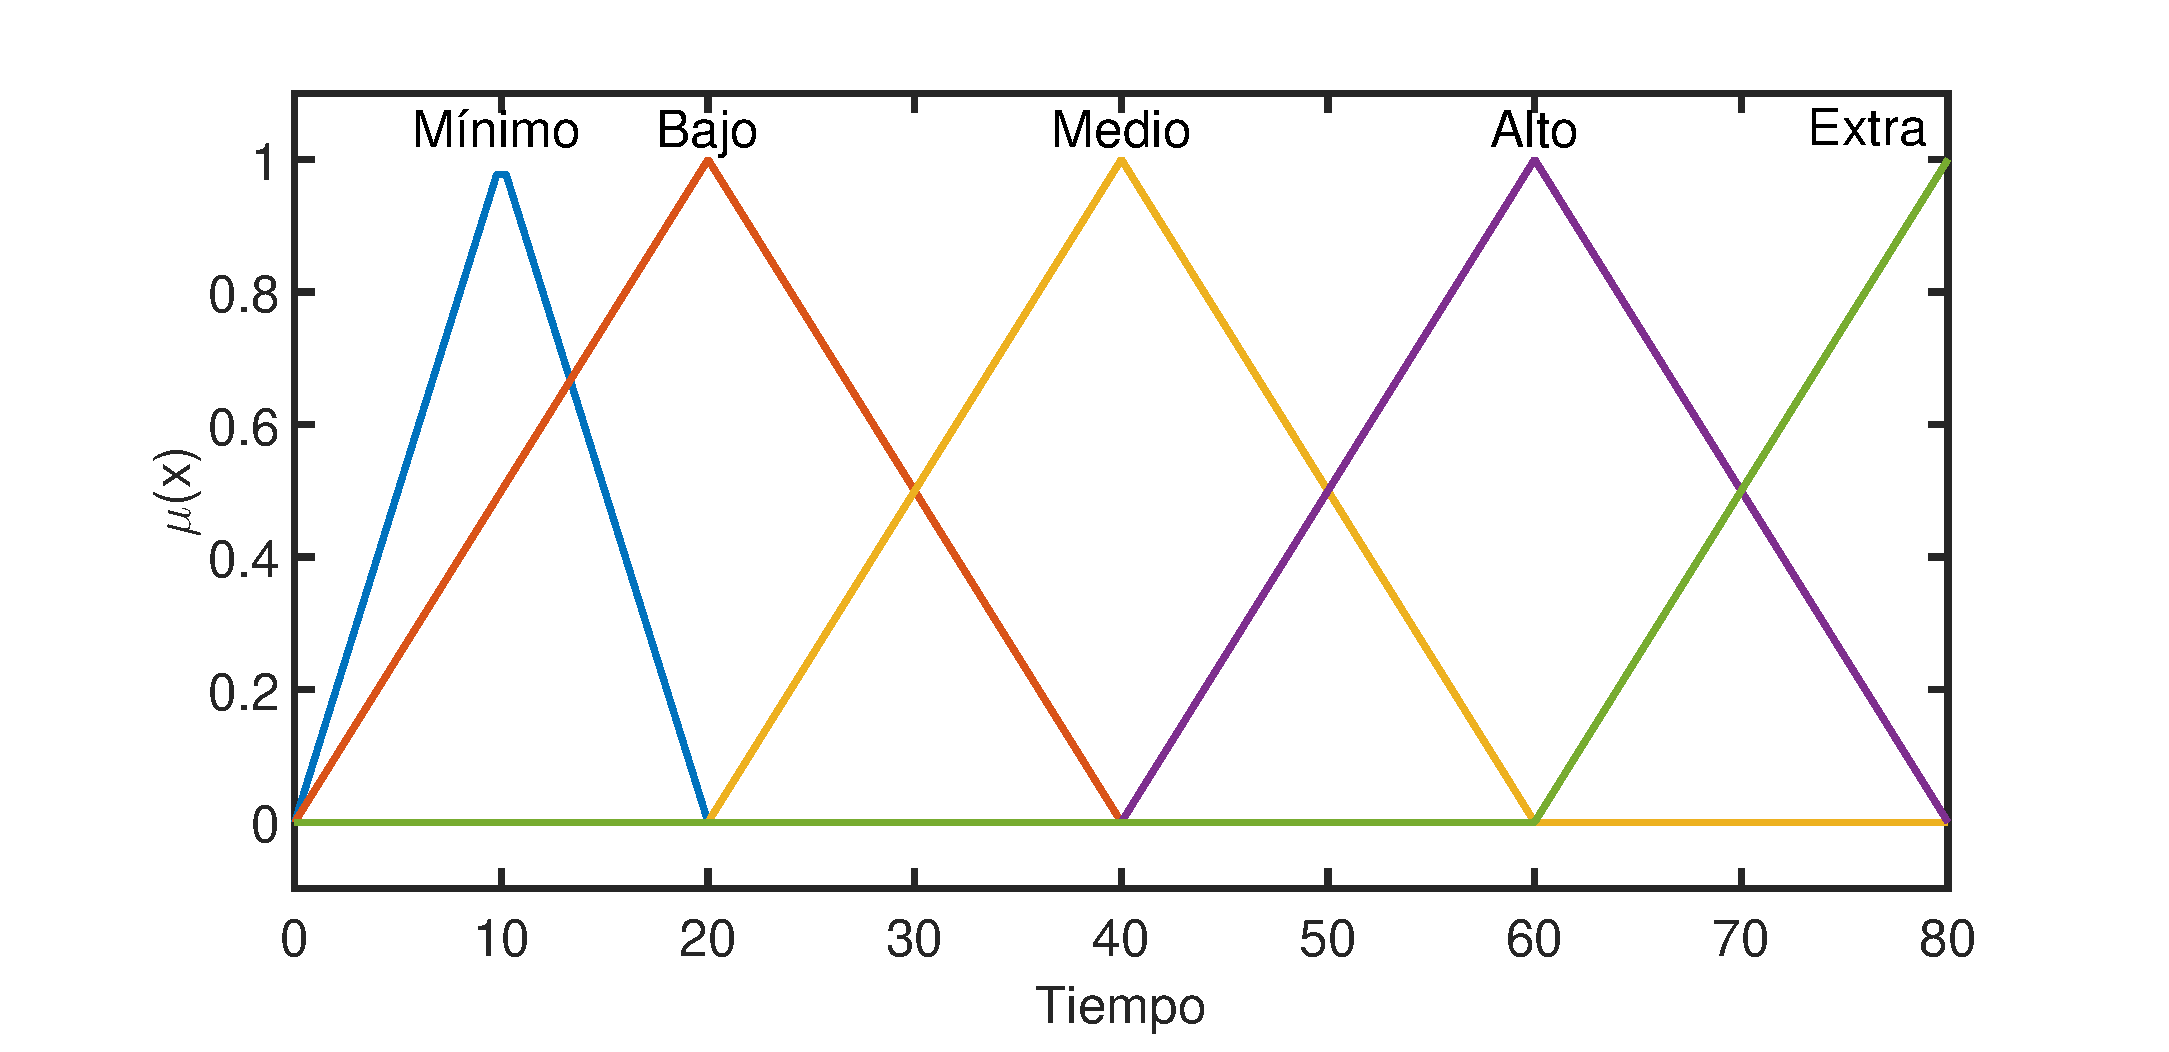
\includegraphics[height=5cm, width=12cm]{Variables/ConfigC_output1.eps}
	\caption[Gráfica variable lingüística tiempo - C]{Representación gráfica de la variable lingüística Tiempo}
\end{figure}

\subsubsection{Base de conocimientos}
El siguiente cuadro muestra las reglas difusas empleadas en esta configuración que se mantiene sin cambios.
\begin{longtable}[c]{lclcl} \toprule
	\multicolumn{3}{c}{Antecedente} & & Consecuente \\ \midrule
	\multicolumn{3}{c}{Vehículos Pocos} & $\rightarrow$ & Verde Mínimo \\
	Vehículos Moderados & Y & Congestión Baja& $\rightarrow$ & Verde Medio \\
	Vehículos Moderados & Y & Congestión Alta& $\rightarrow$ & Verde Bajo \\
	Vehículos Muchos &Y& Congestión Baja& $\rightarrow$ & Verde Extra \\
	Vehículos Muchos &Y& Congestión Alta& $\rightarrow$ & Verde Alto \\ \hline
	\caption{Reglas difusas para la configuración \textit{C}}
\end{longtable}

\pagebreak
\subsubsection{Resultados}
Una vez reajustados los parámetros del sistema de inferencia, se le suministraron lo mismos valores de prueba para evaluar su desempeño respecto a la configuración anterior. Los resultados de dicha evaluación se reflejan en el cuadro siguiente:

\begin{longtable}[c]{cccccc} \toprule
	$V \backslash C$ &  0 & 3 & 6 & 9 & 12 \\ \midrule
	0 & 10.00 & 10.00 & 10.00 & 10.00 & 10.00 \\
	3 & 30.00 & 29.63 & 28.81 & 25.59 & 18.85 \\
	6 & 40.00 & 34.21 & 30.00 & 25.79 & 20.00 \\
	9 & 59.74 & 44.49 & 42.44 & 40.75 & 40.00 \\
	12& 73.33 & 65.87 & 62.38 & 60.59 & 60.00 \\
	\caption{Resultados de la evaluación para la configuración \textit{C}}
\end{longtable}

Donde: la columna V son los valores de prueba de la variable Vehículos, la fila C son los valores de  prueba de la variable Congestión y las celdas son los tiempos (en segundos) obtenidos por la configuración actual.

\subsubsection{Observaciones}
\begin{multicols}{2}

	En esta tercera configuración se aprecia que hubo mejoras considerables en los tiempos inferidos por el sistema. Si se observa la salida para V = 12 y C = 12, cuya salida es 60, se nota que es un tiempo bastante acertado que ayudaría a desahogar la congestión. Por otro lado cuando V = 12 y C = 0, el sistema otorga 13 segundos extra. En el caso contrario, cuando V = 0 y C = 12, el sistema asigna el tiempo mínimo de 10 segundos. Hace falta un nuevo ajuste para saber si los tiempos pueden mejorar aún más.
	
	\begin{figure}[H]
		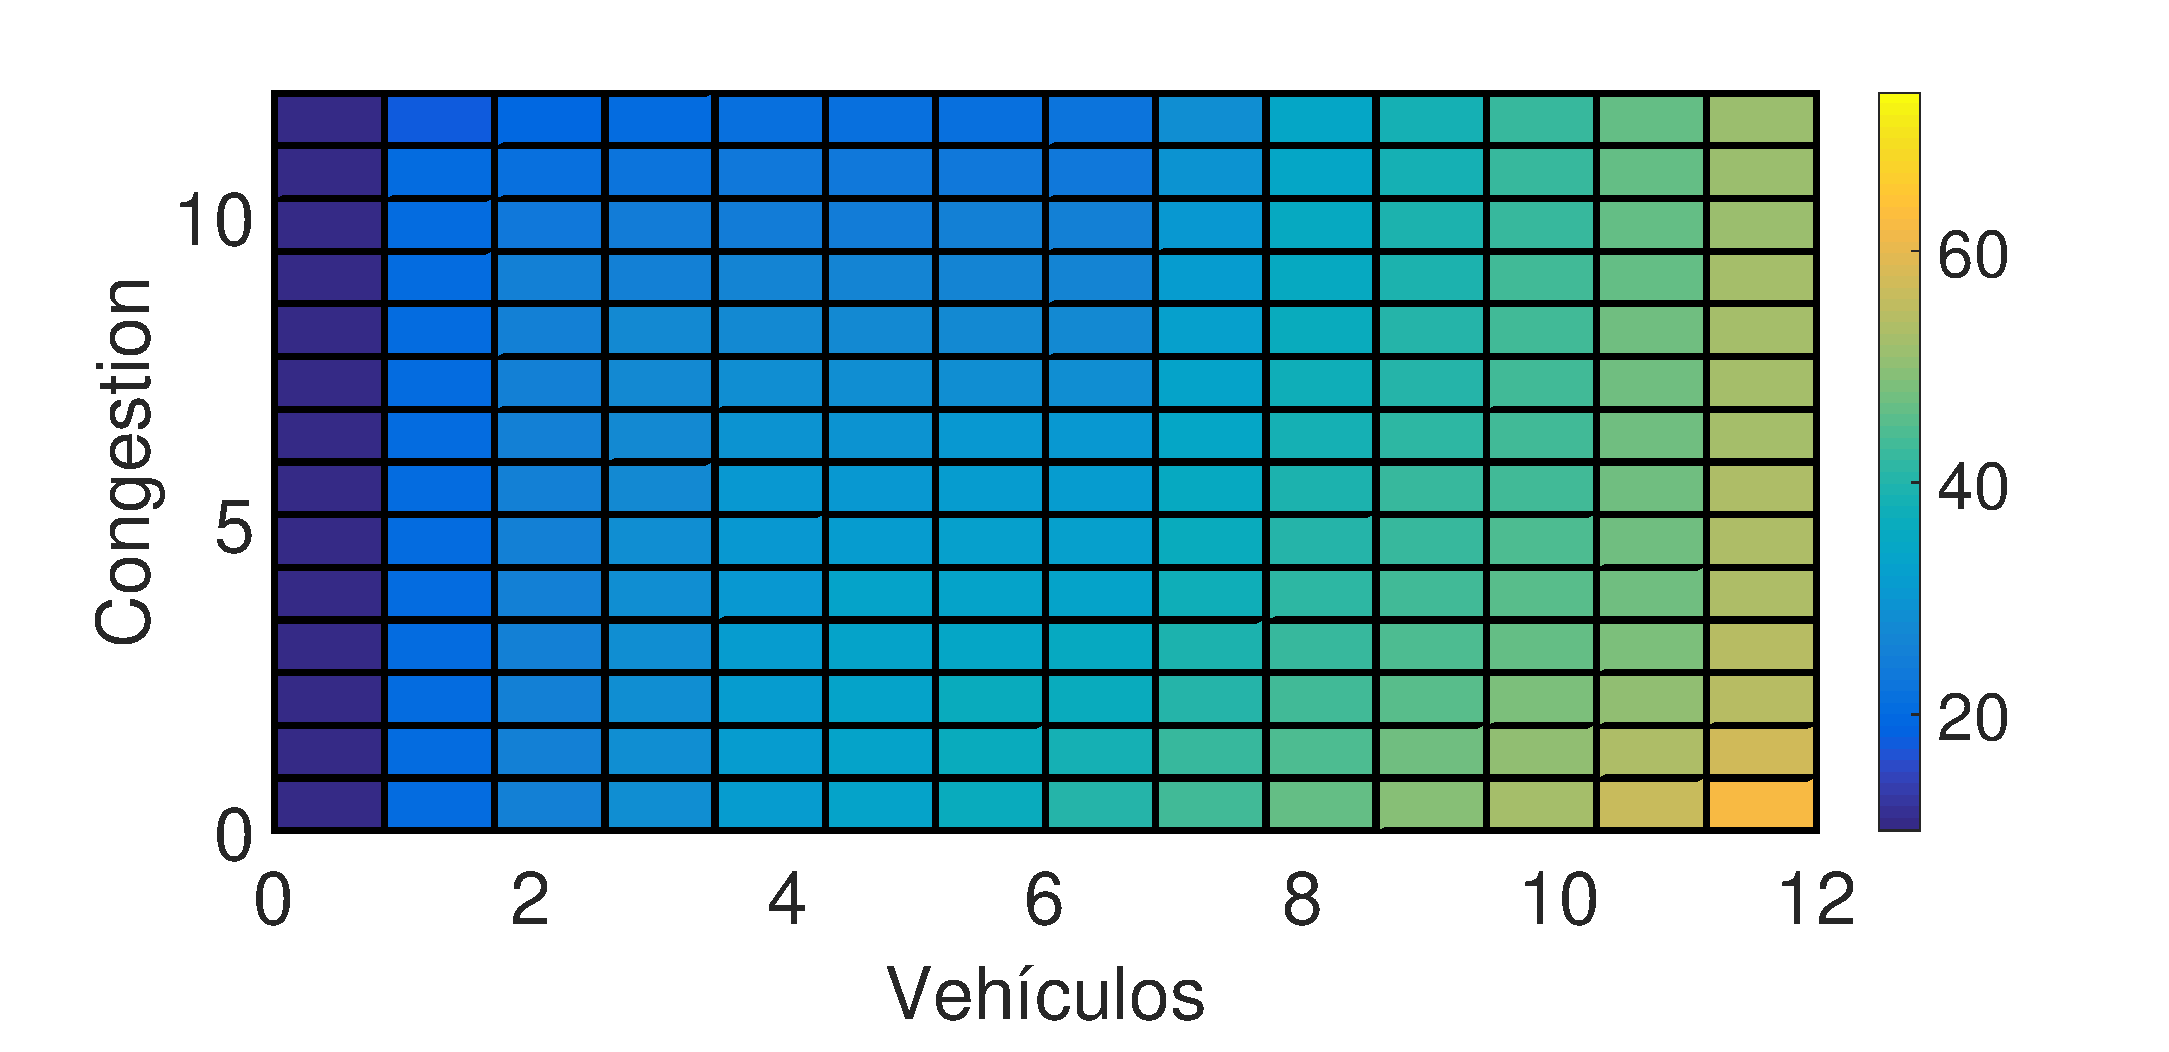
\includegraphics[width=0.5\textwidth]{Surfaces/Surface2D_C.eps}
		\caption{Superficie de control}
	\end{figure}
\end{multicols}
\pagebreak





\subsection{Configuración D}\label{section:configd}
Existen funciones de membresía que modelan mejor el modo de clasificación que realiza la mente humana, estas funciones son las curvas tales como: \textit{Sigmoidales, Gaussianas y Campanas Generalizadas}; en esta configuración se explota el potencial de las primeras dos.

\textbf{Variable de entrada Vehículos.} Las funciones de membresía \textit{triangulares} se remplazan por funciones \textit{Sigmoidales y Gaussianas}, estás modelan de manera más eficiente la manera en que el ser humano suele clasificar los fenómenos.
\begin{center}
	\begin{tabular}{llr} \toprule
		Termino lingüístico & Función de membresía & Parámetros \\ \midrule
		Pocos & Sigmoidal & [ -0.8, 4 ] \\
		Moderados & Gaussiana & [ 1.6, 7 ] \\
		Muchos & Sigmoidal & [ 0.8, 10] \\ \bottomrule
	\end{tabular}
	\captionof{table}{Variable lingüística \textit{Vehículos}}
\end{center}

\textbf{Variable de entrada Congestión.} También se remplaza las funciones triangulares por \textit{funciones Sigmoidales}.

\begin{table}[!h]
	\centering
	\begin{tabular}{llr} \toprule
		Termino lingüístico & Función de membresía & Parámetros \\ \midrule
		Baja & Sigmoidal & [ -0.8, 5 ] \\
		Alta & Sigmoidal & [ 0.8, 5 ] \\ \bottomrule
	\end{tabular}
	\caption{Variable lingüística \textit{Congestión}}
\end{table}
\begin{figure}[H]
	\centering
	\subfigure[Variable lingüística Vehículos]{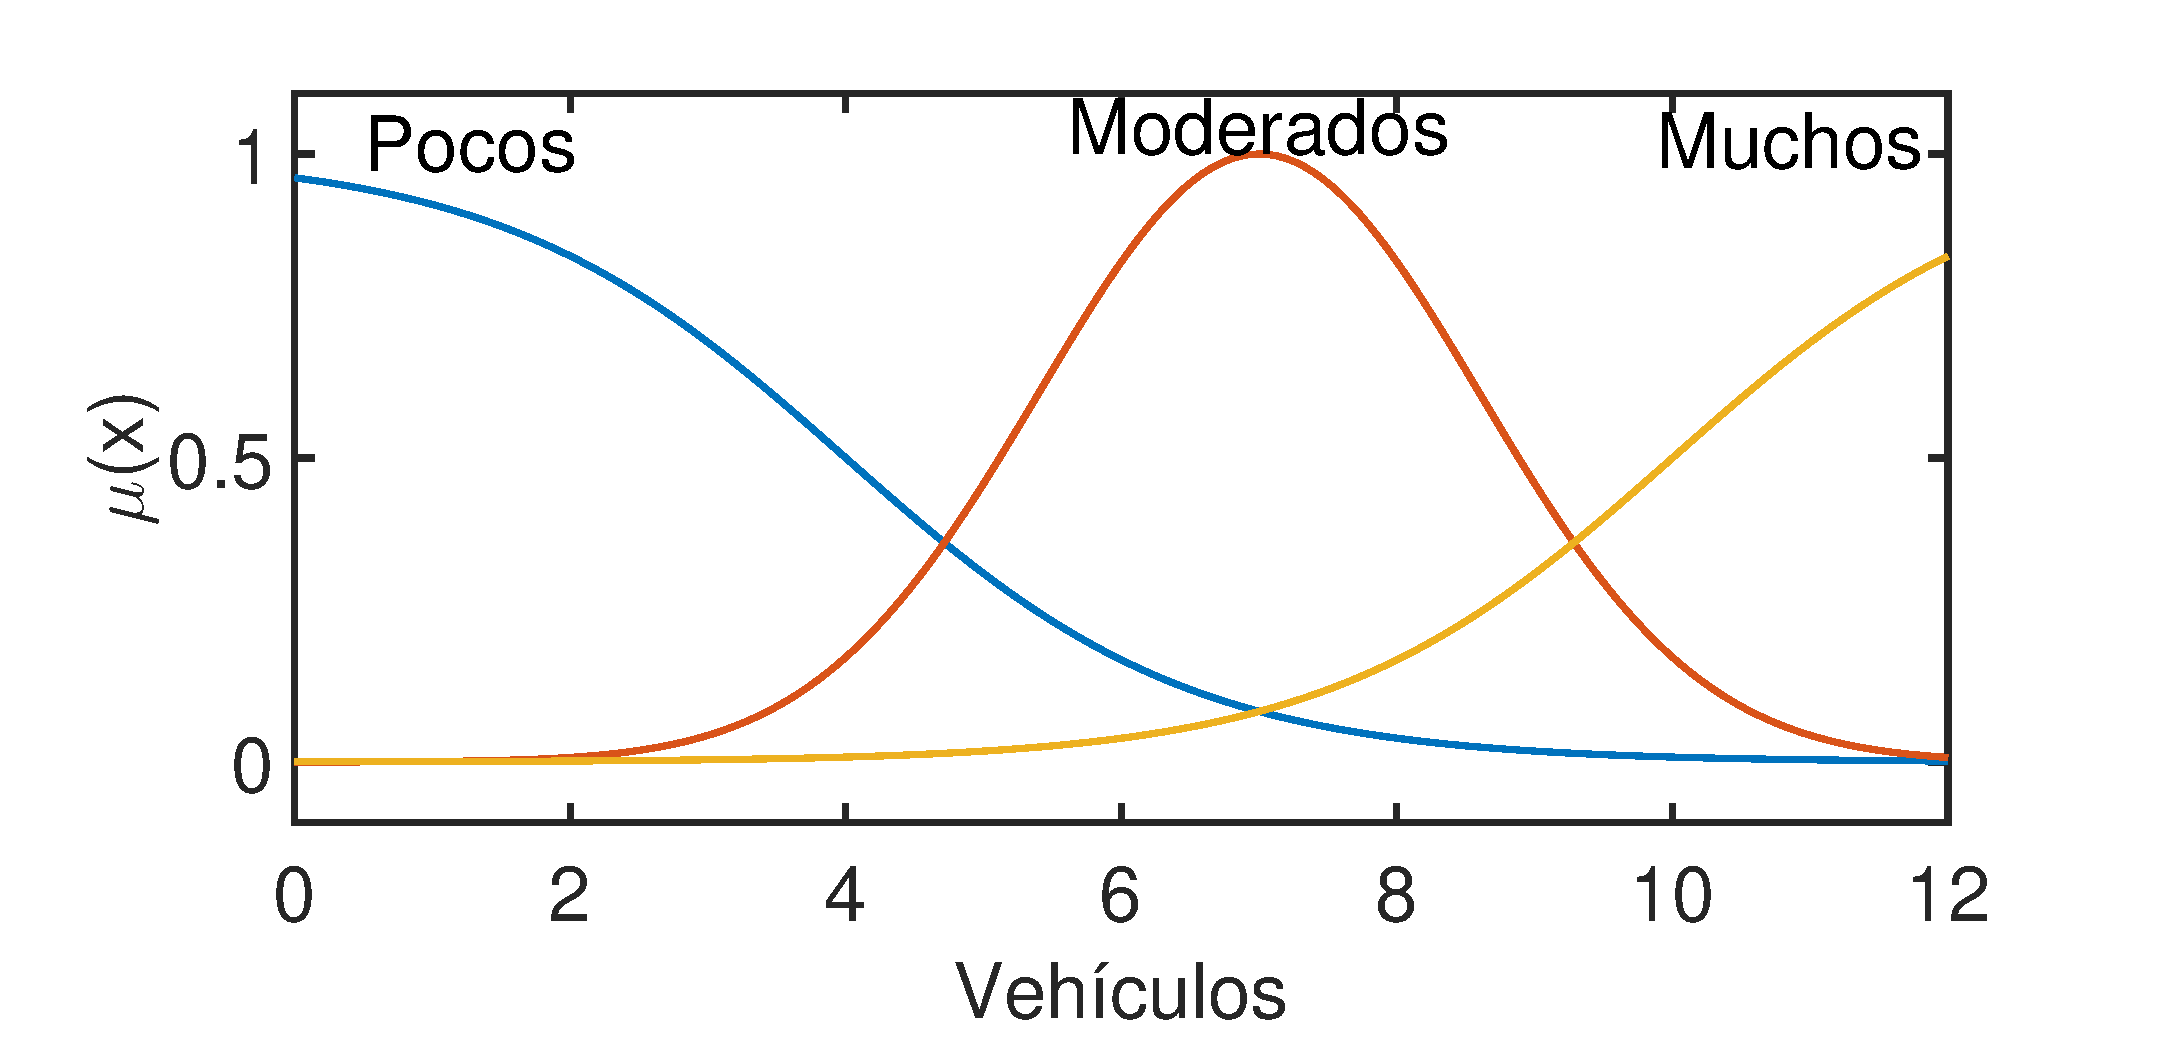
\includegraphics[height=4cm, width=8.1cm]{Variables/ConfigD_input1.eps}}
	\subfigure[Variable lingüística Congestión]{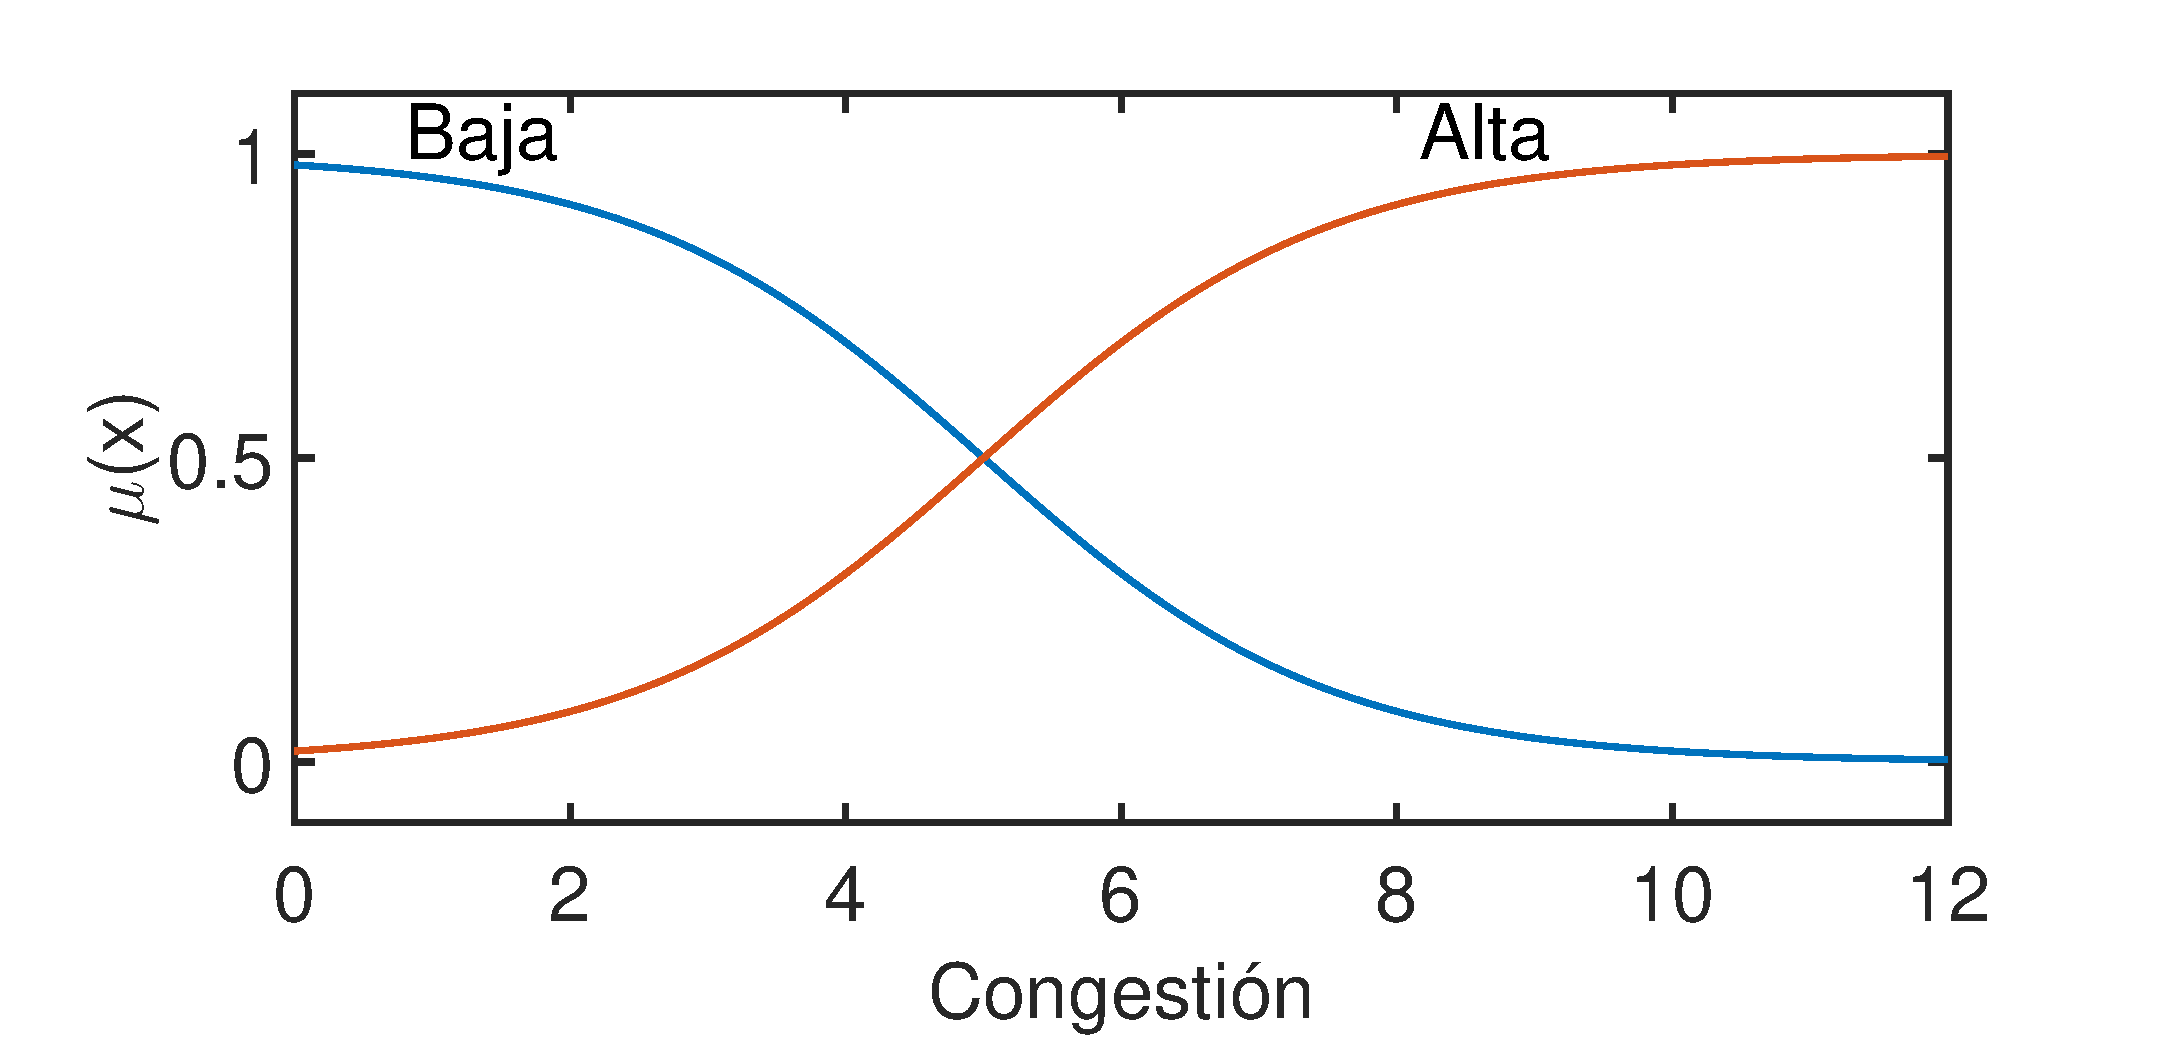
\includegraphics[height=4cm, width=8.1cm]{Variables/ConfigD_input2.eps}}
	\caption[Gráficas de las variables lingüísticas vehículos y congestión]{Representación gráfica de las variables lingüísticas Vehículos y Congestión }
\end{figure}

\textbf{Variable de salida Tiempo.} Esta variable únicamente tiene un ajuste menor en el término lingüístico \textit{Mínimo}, el resto de términos permanece intacto.

\begin{table}[!h]
	\centering
	\begin{tabular}{llr} \toprule
		Termino lingüístico & Función de membresía & Parámetros \\ \midrule
		Mínimo & Triangular & [0, 0, 25 ] \\
		Bajo & Triangular & [0, 25, 40 ] \\
		Medio & Triangular & [20, 40, 60] \\
		Alto & Triangular & [40, 60, 80] \\
		Extra & Triangular & [60, 80, 80] \\ \bottomrule
	\end{tabular}
	\caption{Variable lingüística \textit{Tiempo}}
\end{table}

\begin{figure}[H]
	\centering
	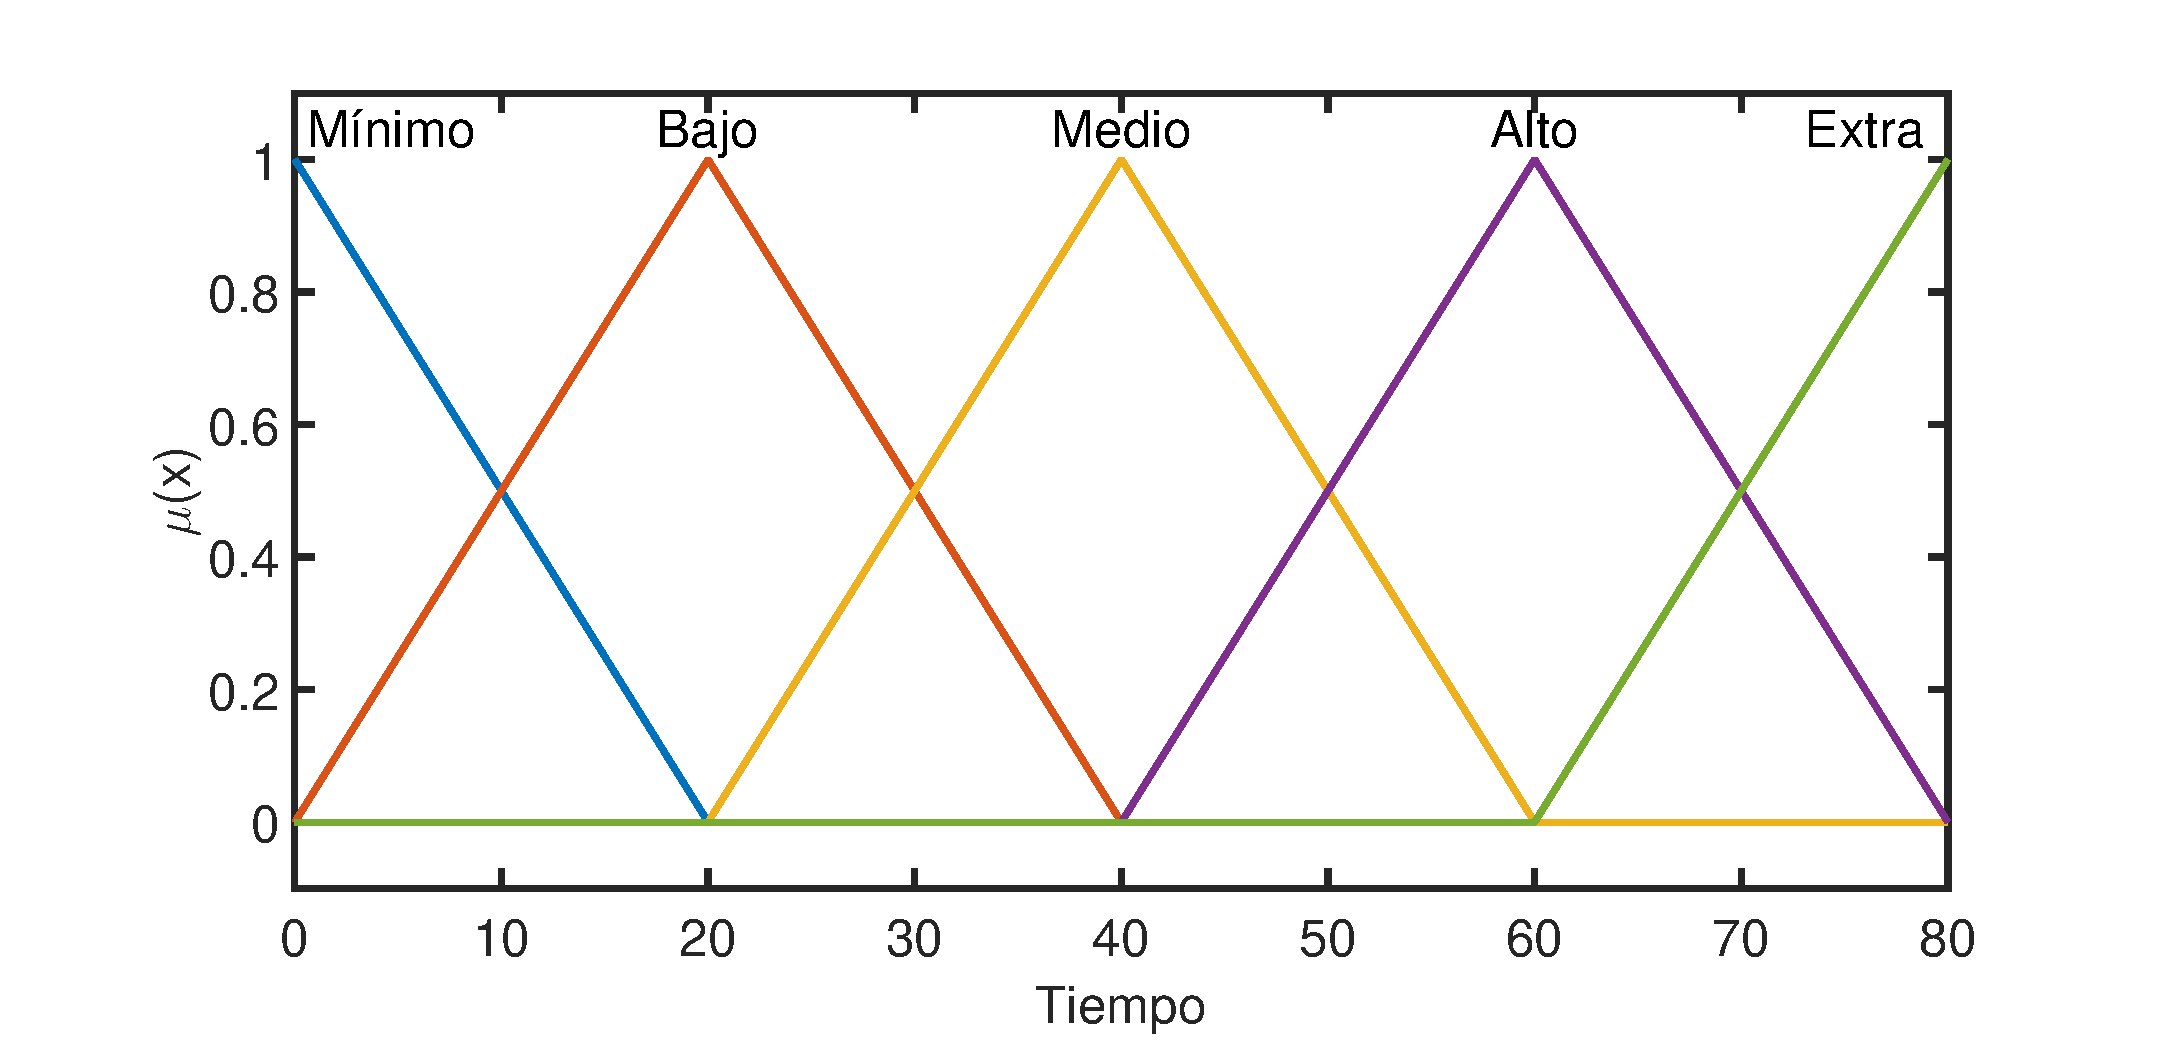
\includegraphics[height=5cm, width=12cm]{Variables/ConfigD_output1.eps}
	\caption[Gráfica variable lingüística tiempo - D]{Representación gráfica de la variable lingüística Tiempo}
\end{figure}

\subsubsection{Base de conocimientos}
El siguiente cuadro muestra las reglas difusas empleadas en esta configuración que se mantiene sin cambios.
\begin{longtable}[c]{lclcl} \toprule
	\multicolumn{3}{c}{Antecedente} & & Consecuente \\ \midrule
	\multicolumn{3}{c}{Vehículos Pocos} & $\rightarrow$ & Verde Mínimo \\
	Vehículos Moderados & Y & Congestión Baja& $\rightarrow$ & Verde Medio \\
	Vehículos Moderados & Y & Congestión Alta& $\rightarrow$ & Verde Bajo \\
	Vehículos Muchos &Y& Congestión Baja& $\rightarrow$ & Verde Extra \\
	Vehículos Muchos &Y& Congestión Alta& $\rightarrow$ & Verde Alto \\ \hline
	\caption{Reglas difusas para la configuración \textit{D}}
\end{longtable}

\pagebreak
\subsubsection{Resultados}
Después de remplazar algunas de las funciones de membresía y realizar los ajustes necesarios, se le suministró los mismos valores de prueba para evaluar su desempeño respecto a la configuración anterior. Los resultados de dicha evaluación se reflejan en el cuadro siguiente:

\begin{longtable}[c]{cccccc} \toprule
	$V \backslash C$ &  0 & 3 & 6 & 9 & 12 \\ \midrule
	0 & 08.41 & 08.41 & 08.41 & 08.41 & 08.41 \\
	3 & 13.25 & 13.25 & 13.25 & 12.98 & 10.85 \\
	6 & 36.56 & 36.54 & 28.81 & 24.08 & 24.02 \\
	9 & 47.81 & 43.60 & 39.23 & 37.65 & 37.62 \\
	12& 70.83 & 66.58 & 60.27 & 59.40 & 59.39 \\
	\caption{Resultados de la evaluación para la configuración \textit{D}}
\end{longtable}

Donde: la columna V son los valores de prueba de la variable Vehículos, la fila C son los valores de  prueba de la variable Congestión y las celdas son los tiempos (en segundos) obtenidos por la configuración actual.

\subsubsection{Observaciones}

\begin{multicols}{2}
	Definitivamente, los resultados obtenidos tras remplazar las funciones triangulares por funciones sigmoidales y gaussianas, son mucho más acertadas. Al principio, los tiempos asignados incrementan más rápido conforme más se eleva el número de autos, después, el ritmo de crecimiento de los tiempos de asignación desacelera al acercarse al valor máximo para las variables de entrada. Se concluye que la configuración actual será la usada en la implementación.
	\begin{figure}[H]
	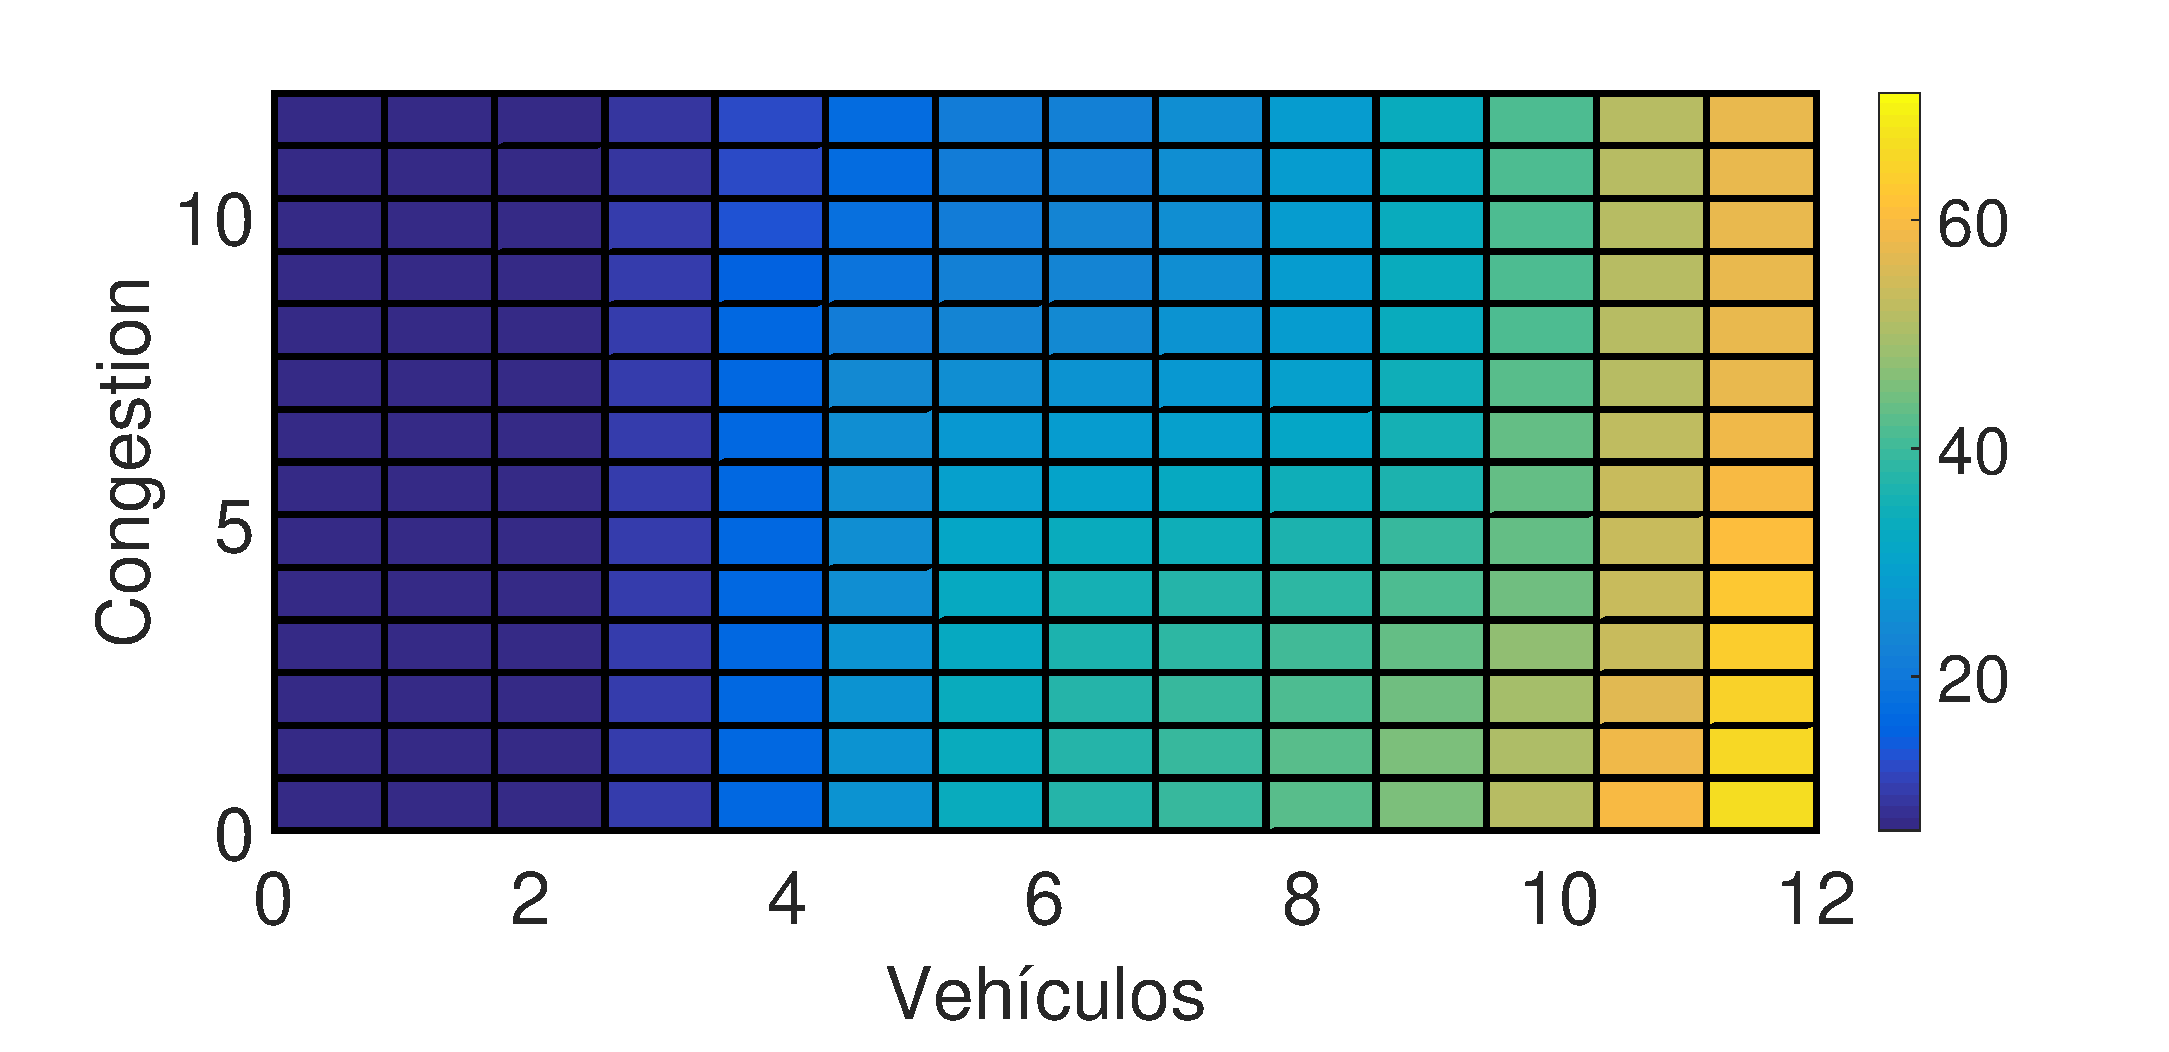
\includegraphics[width=0.5\textwidth]{Surfaces/Surface2D_D.eps}
	\caption{Superficie de control}
\end{figure}
\end{multicols}
\pagebreak

\section{Desarrollo del algoritmo}\label{section:desarrolloAlgoritmo}
Después de haber culminado el desarrollo del sistema de inferencia, el cual representa el componente principal del proyecto, ahora el desarrollo continúa con el algoritmo de sincronización de semáforos.

El modelo propuesto, es a su vez un marco de trabajo para la implementación última, por parte del usuario final.

A lo largo de las siguientes páginas se modela el desarrollo del algoritmo mediante diagramas UML, empleando solo aquellos diagramas que ayuden a tener una perspectiva general del proyecto:
\begin{itemize}
	\item \textbf{Diagrama de actividades} del flujo general del sistema.
	\item \textbf{Diagrama de clases} de todo el sistema.
	\item \textbf{Diagrama de secuencia} del bucle principal.
\end{itemize}

\begin{figure}[H]
	\centering
	\begin{tikzpicture}
	[node distance=10mm and 15mm,
	 legend/.style={pos=0.4, font=\scriptsize, fill=white},
	 block/.style={rectangle,draw=black,fill=yellow!20,thin,minimum height=10mm, minimum width=43mm, font=\footnotesize},
	 rline/.style={->, shorten >= 1pt, >= stealth', semithick,draw=black},]
	 	\node[block] (cam) {Sensor Vehiculos {\scriptsize (e.g. Cámara)} };
		\node[block] (in) [below=of cam] {Entradas {\scriptsize (e.g. Congestión)}};
		\node[block] (fis) [below=of in] {Sistema Difuso};
		\node[block] (out) [below=of fis] {Salidas {\scriptsize (e.g. Tiempo)}};
		\node[block] (sem) [below=of out] {Semáforo ``Inteligente''};

		\node[block] (rules) [left=of fis] {Reglas Difusas};
		\node[block] (vars) [right=of fis] {Variables Lingüísticas};

		\draw [rline] (cam) -- node[legend] {Pre-Procesamiento} (in);
		\draw [rline] (in) -- node[legend] {Fuzzificación} (fis);
		\draw [rline] (fis) -- node[legend] {Defuzzificación} (out);
		\draw [rline] (out) -- node[legend] {Post-Procesamiento} (sem);
		
		\draw [rline] (rules) -- (fis);
		\draw [rline] (vars) -- (fis);
	\end{tikzpicture}
	\caption{Diagrama general del sistema}
\end{figure}

\newpage
\subsection{Diagrama de actividades}
El siguiente diagrama muestra a grandes rasgos, el flujo de ejecución general del algoritmo. En él se puede observar el proceso de inicialización y configuración del semáforo y del sensor; además se muestra el bucle principal ``\emph{repetir siempre}'' que se encarga de obtener los datos del sensor, procesarlos y establecer el cambio de fase.

\begin{figure}[H]
	\centering
	\begin{tikzpicture}
		[auto,
		decision/.style	={diamond, draw=blue, thin, fill=yellow!20, text width=5cm, align=flush center, inner sep=1pt},
		bucle/.style	={chamfered rectangle, draw=black, thin, fill=yellow!20, text width=5.5cm, align=flush center, minimum height=2em},
		block/.style	={rectangle, draw=black, thin, fill=yellow!20, text width=5cm, align=center, minimum height=2em},
		line/.style		={draw=black, semithick, -latex', shorten >= 2pt},
		cloud/.style = {draw=red, thick, ellipse, fill=red!20, minimum height=2em}
		]
		\node at (-6.3cm,0) {Main};
		\node at (0,0) {Semáforo};
		\node at (6.3cm,0) {Sensor};
		
		\draw [dashed] (-3.25cm,0) -- +(0,-15cm);
		\draw [dashed] (3.25cm,0) -- +(0,-15cm);
		\draw (-9cm,0.5cm) rectangle (9cm,-15.1cm);
		\matrix[column sep=5mm, row sep=5mm, anchor=north] at (0,-1)
		{
			\node [block] (init)	{Inicio}; & &\\
			\node [block] (setupconfig)	{Inicializar Configuración}; & &\\
			\node [block] (setupsensor)	{Inicializar Sensor}; & &\\
			\node [block] (setupsemaforo)	{Inicializar Semáforo}; && \\
			\node [block] (runsemaforo) {Iniciar Semáforo}; & &\\
			& \node [bucle] (repetir) {Repetir siempre}; & \\
			& & \node [block] (contar) {Contar vehículos};\\
			& \node [block] (preprocesar)	{Preprocesar Datos}; & \\
			& \node [block] (inferir)	{Inferir Tiempo}; & \\
			& \node [block] (establecer)	{Establecer Fase}; & \\
		};

		\begin{scope}[every path/.style=line]
			\path	(init) -- (setupconfig);
			\path	(setupconfig) -- (setupsensor);
			\path	(setupsensor) -- (setupsemaforo);
			\path	(setupsemaforo) -- (runsemaforo);
			\path	(runsemaforo) -| (repetir);
			\path	(repetir) -| (contar);
			\path	(contar) |- (preprocesar);
			\path	(preprocesar) -- (inferir);
			\path	(inferir) -- (establecer);
			\path	(establecer) -- +(-6,0) |- (repetir);
		\end{scope}
	\end{tikzpicture}
	\caption{Diagrama de actividades general}
\end{figure}
\newpage


\subsection{Diagrama de secuencia}
\textbf{Diagrama de secuencia del bucle de control del semáforo}\\
En el diagrama anterior se muestra el bucle principal del sistema, ahora mediante un diagrama de secuencia se detallarán dicho bucle debido a que es la parte central del sistema.

Para fines de legibilidad, en el siguiente diagrama se omiten los nombres de las clases (\emph{FuzzySemaforo y SensorVehiculos}). Las funciones que se muestran pertenecen a la clase \emph{FuzzySemaforo} excepto una, la cual está indicada en el diagrama.
\begin{figure}[H]
	\centering
	\tikzumlset{font=\small, call dt=9, call padding=4}
	\begin{tikzpicture}
	\begin{umlseqdiag}[]
	\umlobject[]{run}
	\umlobject[x=5]{read}
	\umlobject[x=7.0]{getMedia}
	\umlobject[x=9.2]{getTime}
	\umlobject[x=11.4]{setLights}
	
	\begin{umlfragment}[type=loop, label=para cada fase, inner xsep=10]
	\begin{umlcall}[op=read(), return={autos : vector<int>}]{run}{read}\end{umlcall}
	\begin{umlcall}[op={get\_media(fase,vehiculos)}, return=vehículos : double]{run}{getMedia}\end{umlcall}
	\begin{umlcall}[op={get\_media(fase,congestión)}, return=congestión : double]{run}{getMedia}\end{umlcall}
	\begin{umlcall}[op=infiere tiempo en verde, return=segundos : double, name=call]{run}{getTime}\end{umlcall}
	\begin{umlcall}[op=establece la siguiente fase]{run}{setLights}\end{umlcall}
	\end{umlfragment}
	\umlnote[x=10, y=-3]{read}{Función miembro de la clase MySensor}
	%\umlnote[x=11, y=-6]{call-1}{Llamada al Sistema de Inferencia Difusa}
	\end{umlseqdiag}
	\end{tikzpicture}
	\caption{Diagrama de secuencia del bucle principal}	
\end{figure}


\subsection{Diagrama de clases}\label{subsection:umlclases}
\textbf{Modelado de las \textit{relaciones de clase} del sistema}\\
En el siguiente diagrama se modela las clases que constituyen el sistema además, se muestran las diferentes relaciones que existen entre dichas clases.

Para mayor legibilidad, el diagrama no modela atributos ni comportamientos de las clases; sin embargo, en el apéndice \ref{apendice:a} se modelan los elementos omitidos.
\begin{figure}[h]
\begin{tikzpicture}

\umlsimpleclass[y=-2.5]{MySemaforo}
\umlsimpleclass[x=-6.6, y=0]{FuzzySet}
\umlsimpleclass[x=6.5, y=-2.5]{MySensor}
\umlsimpleclass[type=abstract]{FuzzySemaforo}

\umlsimpleclass[x=-4, y=3.5]{TriangularMF}
\umlsimpleclass[x=0, y=3.5]{SigmoidalMF}
\umlsimpleclass[x=4, y=3.5]{GaussianaMF}

\umlsimpleclass[x=-6.6, y=7]{FuzzyValue}
\umlsimpleclass[x=0, y=7, type=abstract]{MembershipFunction}
\umlsimpleclass[x=6.5, y=7, type=abstract]{SensorVehiculos}

\umlunicompo[geometry=|-|, anchor1=140, mult1=1, mult2=0..*, pos2=2.8]{FuzzySemaforo}{TriangularMF}
\umlunicompo[geometry=|-|, anchor1=90, mult1=1, mult2=0..*, pos2=2.8]{FuzzySemaforo}{SigmoidalMF}
\umlunicompo[geometry=|-|, anchor1=40, mult1=1, mult2=0..*, pos2=2.8]{FuzzySemaforo}{GaussianaMF}

\umlunicompo[mult1=1, pos1=0, align1=right, mult2=0..*, pos2=1, align2=left]{FuzzySemaforo}{FuzzySet}
\umluniassoc[geometry=-|, anchor2=-130, attr2=cuenta vehículos|1, pos2=1, align2=right, align1=left, mult1=1, pos1=0]{FuzzySemaforo}{SensorVehiculos}
\umlimpl[geometry=|-|]{TriangularMF}{MembershipFunction}
\umlimpl[geometry=|-|]{SigmoidalMF}{MembershipFunction}
\umlimpl[geometry=|-|]{GaussianaMF}{MembershipFunction}

\umlimpl{MySensor}{SensorVehiculos}
\umluniassoc[mult1=1, pos1=0, align1=right, mult2=0..1, pos2=1, align2=left]{MembershipFunction}{FuzzyValue}
\umluniassoc[mult1=1, pos1=0.05, mult2=0..1, pos2=1, align2=left]{FuzzySet}{FuzzyValue}	

\umlimpl{MySemaforo}{FuzzySemaforo}
\end{tikzpicture}
\caption{Diagrama de clases del sistema}
\label{uml:relaciones}
\end{figure}
%\newpage
%\textbf{Diagrama de actividades que modela el proceso de inferencia}


\chapter{Desarrollo}

En este capítulo se describe el desarrollo del sistema en general: la selección de la técnica, el desarrollo de la técnica seleccionada y la selección del lenguaje de programación.

A continuación, en la \textbf{sección \ref{section:selecciontecnica}} se describe, a manera de resumen: las diferentes técnicas tomadas en cuenta durante la investigación y los porqués de la técnica seleccionada.

Después en la \textbf{sección \ref{section:desarrolloFIS}}, se describe el proceso de diseño del \textit{Sistema de Inferencia Difuso} bajo una metodología de mejora iterativa. El sistema tiene como objetivo calcular el tiempo de la fase en verde de un semáforo, que mediante la estructura propuesta y un preprocesamiento de los datos, permitirá gestionar diferentes tipos de intersecciones.

Posteriormente en la \textbf{sección \ref{section:desarrolloAlgoritmo}} se modela, mediante diagramas UML, la arquitectura del software desarrollado. El resultado es una micro-librería que permite \emph{expresar las variables y reglas del sistema difuso en notación de objetos}. Además, se modela la estructura propuesta para integrar la técnica seleccionada, a un sistema de control (a un algoritmo de sincronización) de semáforos y así, posibilitar la aplicación del sistema a una intersección con número no-estático de avenidas y fases.

\section{Preliminares}
Antes de continuar con el diseño del sistema, se considera adecuado aclarar algunos puntos acerca de:

\paragraph{El enfoque}presentado en este proyecto difiere con el resto en que, fue diseñado para ser embebido dentro de un algoritmo de sincronización de semáforos más general, de esta manera la tarea del \textit{FIS} se centra en determinar el tiempo en verde, dejando los detalles de sincronización en manos de un segundo algoritmo (también propuesto y desarrollado en este proyecto).

%El segundo algoritmo se encarga no solo del \emph{pre} y \emph{post} procesamiento de los datos de entrada y salida, sino que también define un marco de trabajo para la implementación final por parte del usuario final, valga la redundancia.

\paragraph{El pre-procesamiento} de los datos permite, mediante un proceso matemático sencillo, adaptar el \emph{FIS} propuesto a cruces con un número arbitrario de avenidas y fases, por ejemplo, intersecciones de: 2 avenidas y 2 fases, 4 avenidas y 2 fases o 4 avenidas y 4 fases. De esta manera se logra integrar una técnica de inteligencia artificial con un segundo algoritmo para la sincronización de semáforos.

%\paragraph{Lenguaje de programación}



\begin{wrapfigure}{r}{4cm}
	
\includegraphics[width=4cm]{Sources/logo_cpp11.jpg}
	\captionof{figure}{C++ 11}
\end{wrapfigure}

\paragraph{La elección del lenguaje de programación} para la implementación del algoritmo fue bastante sencilla. Se requería un lenguaje eficiente que permitiera tener un control fino del proceso de inferencia, además de que permitiera que el algoritmo fuese portable entre plataformas. Por ello, se optó por el lenguaje de programación \emph{C++}, en específico, el estándar \emph{ISO C++11}.

C++ es uno de los más eficientes, con herramientas como punteros y referencias que evitan el desperdicio de memoria además de la \emph{semántica de movimiento} incluida en el estándar \textsc{C++11} que, aligera el paso de objetos de gran tamaño entre funciones (como los vectores usados en el proceso de inferencia). Por lo dicho anteriormente y por su amplia disponibilidad de compiladores en casi todas las plataformas, C++ resulta la elección perfecta para este proyecto.

C++ es un lenguaje \textbf{multiparadigma}, permite trabajar usando programación estructurada, orientada a objetos e incluso funcional. En este proyecto se decidió hacer uso del paradigma orientado a objetos, debido a que se busca crear piezas de software altamente reutilizables y expresivas.

\section{Selección de la técnica}\label{section:selecciontecnica}
Después de investigar acerca de las principales ramas de la Inteligencia Artificial (véase sección \ref{cap:ramasdelaia}), se decidió optar por el uso de una técnica de Lógica Difusa; a saber, un \emph{Sistema Inferencia Difusa (FIS por sus siglas en inglés)}. Cabe mencionar que esta técnica está siendo ampliamente usada en la optimización del tráfico vehicular (véase la tabla \ref{table:estadodelarte}), esto se debe en parte, a que permite razonar sobre términos imprecisos como ``\emph{muchos carros}'' o ``\emph{poca congestión}''.

La elección de esta técnica sobre las otras se debe a varios factores: 

\textbf{a) Algoritmos genéticos.} Son una buena opción ya que podrían permitir probar diferentes asignaciones de tiempo, evaluar su desempeño y, así, ir depurando hasta encontrar la configuración optima de tiempos. Sin embargo, debido que la evaluación del desempeño podría ocasionar una congestión bastante alta, no es factible evaluarlo en un entorno real. Otra opción es evaluar el algoritmo en un entorno simulado, por desgracia, el tiempo requerido para la desarrollo del AG, del entorno de simulación y su correspondiente modelo matemático, va más allá del disponible para este proyecto.

\textbf{b) Redes neuronales artificiales.} Estas son de gran ayuda en tareas como reconocimiento de voz, clasificación automática, tratamiento de imágenes entre otros. Sin embargo, desarrollar de una RNA para determinar el cambio de fase de un semáforo, podría llevar a lidiar con dificultades innecesarias, dificultades inherentes al entrenamiento de la propia red.

\textbf{c) Sistemas expertos.} A primera vista puede parecer una buena idea, sin embargo, los problemas vienen al momento de expresar el conocimiento del experto en términos cuantitativos ya que no es muy fácil decidir en qué punto se le debe ceder el paso a una avenida u otra.

Una variante, son los sistemas difusos. Aquí sucede algo importante: los controladores difusos y los sistemas expertos difusos son en esencia lo mismo: Sistema de Inferencia Difusa. Es decir, ambos se basan en la inferencia difusa, por ejemplo: la inferencia de mamdani.

\textbf{d) Sistema de inferencia difusa.} La gran ventaja de estos sistemas es que, gracias a que usan lógica difusa, permiten expresar el conocimiento (reglas) en términos coloquiales que poseen cierto grado de incertidumbre. Así, es posible modelar un sistema que de preferencia a las avenidas con muchos carros y, definir el término muchos carros con una función de membresía centrada en 7. De esta manera, entre más cercano sea a 7 el valor evaluado, mayor peso tendrá en la decisión tomada por el sistema.

Estos sistemas permiten lidiar con la información que no es tan precisa o, en el caso de este proyecto, permite razonar sobre términos como \textit{``muchos carros''} o \textit{``poca congestión''}. Términos para los cuales, no es fácil asignar un intervalo de valores. Es por eso que se decidió usar un Sistema de Inferencia Difusa para dotar de cierto grado de ``inteligencia'' a un algoritmo de control de semáforos.

\section{Diseño del sistema de inferencia}\label{section:desarrolloFIS}
En esta sección se expone de manera metodológica las diferentes configuraciones, resultados y conclusiones que se obtuvieron en el desarrollo del sistema. Para la configuración se sigue una estrategia de mejora iterativa hasta alcanzar el resultado deseado.

\subsection{Configuraciones aplicadas de manera general}
\textbf{Selección del método de inferencia}\\
Se optó por el método de \textbf{Mamdani} debido a que emula mejor el razonamiento humano.

\textbf{Selección de operadores}\\ 
Debido a la variedad de operadores que pueden ser usados en la inferencia difusa, a continuación se muestran los operadores usados en este proyecto.

\begin{multicols}{2}
\begin{itemize}
	\item \textbf{Método AND:} operador mínimo \emph{min}.
	\item \textbf{Método OR:} operador máximo \emph{max}.
	\item \textbf{Implicación:} operador mínimo \emph{min}.
	\item \textbf{Agregación:} operador máximo \emph{max}.
	\item \textbf{Defuzzificación:} centroide \emph{$\frac{\sum \mu(x).x}{\sum \mu(x)}$}.
\end{itemize}
\end{multicols}
\newpage
\subsubsection{Selección de variables}
Como se mencionó, el diseño del sistema difuso, se enfoca en el cálculo de tiempos óptimos para las fases verdes de los semáforos, para ello, se consideran tres aspectos, a saber: la cantidad de autos a los que se les cederá el paso, la cantidad de autos que quedarán en espera y, el número de carriles por avenida. Estos datos permitirán al sistema de inferencia dar preferencia a aquellas avenidas con un mayor número de carriles y/o mayor número de autos.

La selección de variables de entrada y salida del sistema, debe ser cuidadosa para no elevar la complejidad del sistema ni caer en redundancias. En el desarrollo de este sistema se ha seguido la filosofía KISS\footnote{Keep it simple, Stupid!} que plantea el desarrollo de sistemas sencillos, flexibles y escalables.

Al seleccionar las variables hay que cuidar que estás estén correlacionadas con las variables de salida, además, se debe mantener el número de variables y particiones al mínimo necesario.

Habiendo dicho lo anterior, se presenta la selección de variables, así, como una breve justificación de su elección. \\

\textbf{Variables de entrada}\\
\textit{a) Vehículos.} La variable vehículos indica la cantidad de autos que se encuentran en la avenida a la que se le dará el paso.\\
\textit{b) Congestión.} La variable congestión se propone como un indicador que sume de manera ponderada la cantidad de automóviles y carriles. A saber, la suma ponderada se define como:

\begin{displaymath}
\frac{\sum_{i=1}^{n} x_i * w_i}{\sum_{i=1}^{n} w_i}
\end{displaymath}
Donde:

{\setlength{\baselineskip}{0.7\baselineskip}\begin{description}
	\item $x$ es un vector con la cantidad de autos de las avenidas.
	\item $w$ es un vector de pesos que describe la prioridad de cada avenida.
\end{description}}

Además, se propone el cálculo de los pesos de las avenidas como una función directamente proporcional al número de carriles de la avenida en cuestión e inversamente proporcional al número total de carriles , i,e:

\begin{displaymath}
w_i = \frac{ c_i }{\sum_{j=1}^{j=n} c_j}
\end{displaymath}
Donde:
{\setlength{\baselineskip}{0.7\baselineskip}\begin{description}
		\item $C$ es un vector con la cantidad de carriles de cada avenida.
		\item $i$ es la avenida a evaluar.
\end{description}}
De esta manera el sistema resulta lo suficientemente flexible para ser aplicado a intersecciones de 2, 4, 8 o cualquier numero $n$ de avenidas (siempre y cuando tenga sentido).\\

\textbf{Variables de salida}\\
\textit{a) Tiempo.} Con el fin de hacer el sistema fácilmente escalable, se propone como variable de salida la cantidad de segundos de la fase verde del semáforo en cuestión. Esto permitirá integrar el sistema de inferencia dentro de un algoritmo clásico de control de semáforos. Así, la \textit{inteligencia} se encuentra en la optima asignación de tiempos.

\newpage
\subsection{Configuración A}
La configuración presentada a continuación mantiene al mínimo el número de términos dentro de las variables de entrada y salida. 

\textbf{Variable de entrada Vehículos.} Referente a la cantidad de vehículos en la avenida a la cual se le asignará la fase verde. La variable se encuentra definida en un universo de discurso $U = [0,12]$.

\begin{table}[!h]
	\centering
	\begin{tabular}{llr} \toprule
		Termino lingüístico & Función de membresía & Parámetros \\ \midrule
		Pocos & Triangular & [0, 0, 12 ] \\
		Muchos & Triangular & [0, 12, 12] \\ \bottomrule
	\end{tabular}
	\caption{Variable lingüística \textit{Vehículos}}
\end{table}


\textbf{Variable de entrada Congestión.} Se refiere al índice ponderado de la cantidad de vehículos en las avenidas que quedaran a la espera durante la fase verde actual. La variable se encuentra definida en un universo de discurso $U = [0,12]$.

\begin{table}[!h]
	\centering
	\begin{tabular}{llr} \toprule
		Termino lingüístico & Función de membresía & Parámetros \\ \midrule
		Baja & Triangular & [0, 0, 12 ] \\
		Alta & Triangular & [0, 12, 12] \\ \bottomrule
	\end{tabular}
	\caption{Variable lingüística \textit{Congestión}}
\end{table}

\begin{figure}[H]
	\centering
	\subfigure[Variable lingüística Vehículos]{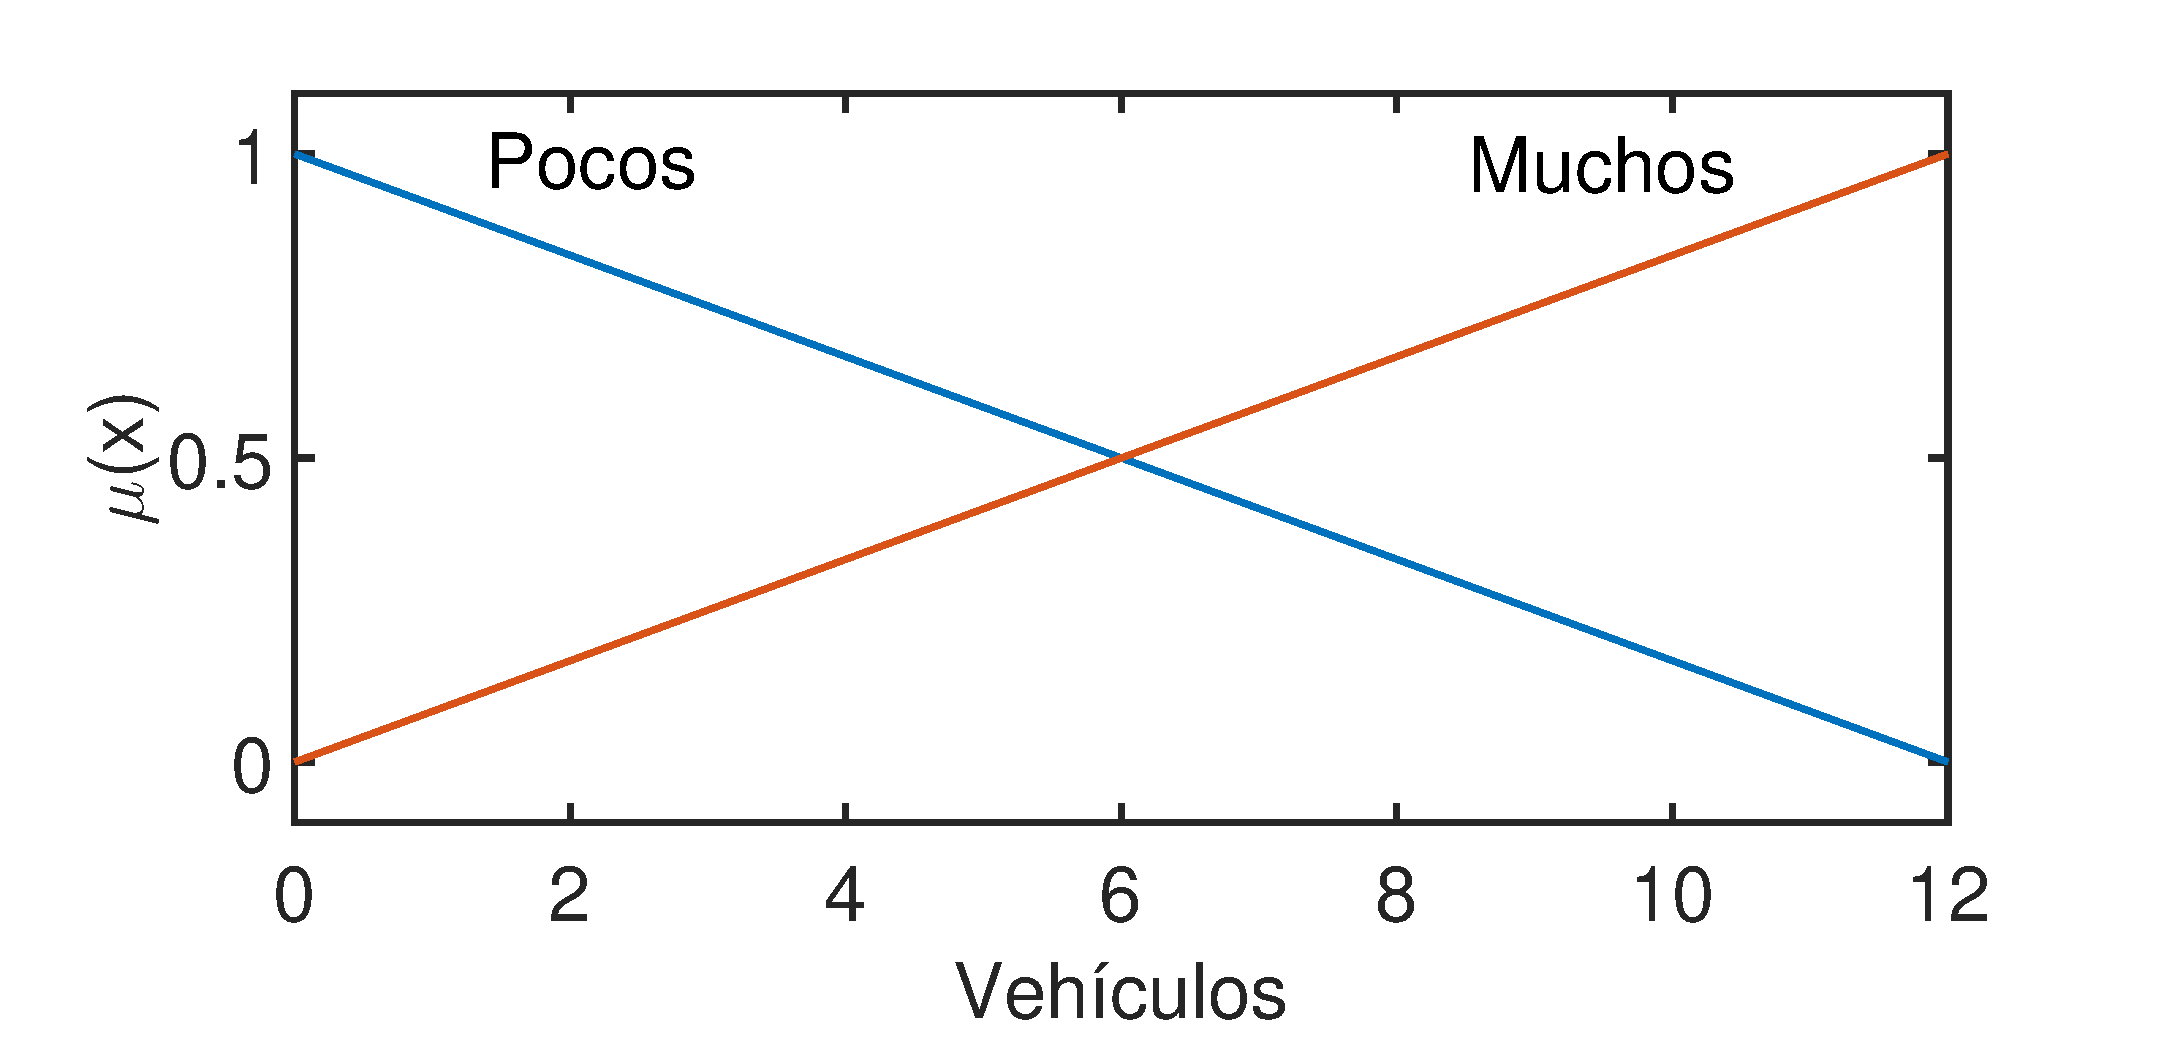
\includegraphics[height=4cm, width=8.1cm]{Variables/ConfigA_input1.eps}}
	\subfigure[Variable lingüística Congestión]{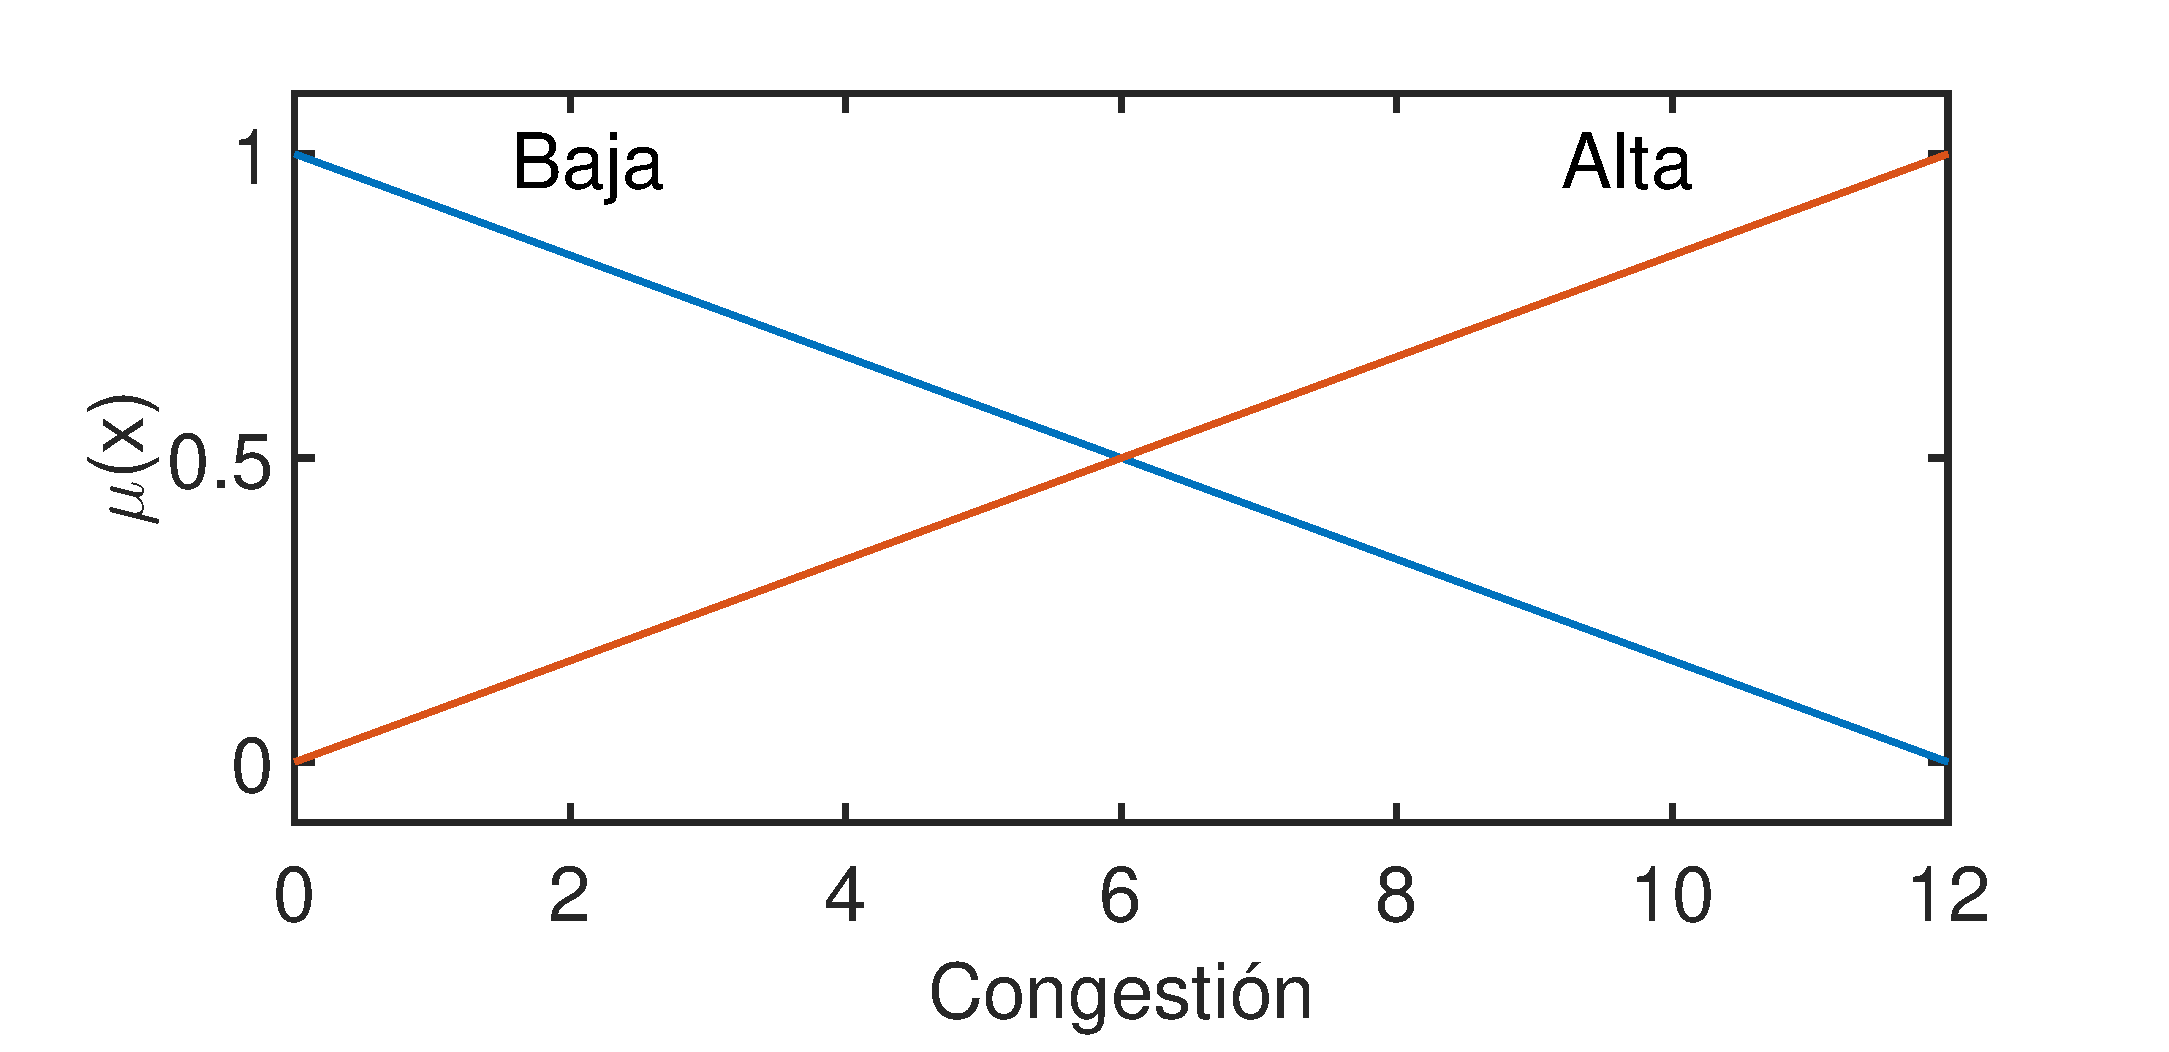
\includegraphics[height=4cm, width=8.1cm]{Variables/ConfigA_input2.eps}}
	\caption[Gráficas de las variables lingüísticas vehículos y congestión]{Representación gráfica de las variables lingüísticas Vehículos y Congestión }
\end{figure}

\newpage
\textbf{Variable de salida Tiempo.} Se refiere al tiempo en segundos que le será asignada a la fase verde actual. La variable se encuentra definida en un universo de discurso $U = [0,90]$.

\begin{table}[!h]
	\centering
	\begin{tabular}{llr} \toprule
		Termino lingüístico & Función de membresía & Parámetros \\ \midrule
		Bajo & Triangular & [0, 0, 30 ] \\
		Medio & Triangular & [0, 30, 60] \\
		Moderado & Triangular & [30, 60, 90] \\
		Alto & Triangular & [60, 90, 90] \\ \bottomrule
	\end{tabular}
	\caption{Variable lingüística \textit{Tiempo}}
\end{table}

\begin{figure}[H]
	\centering
	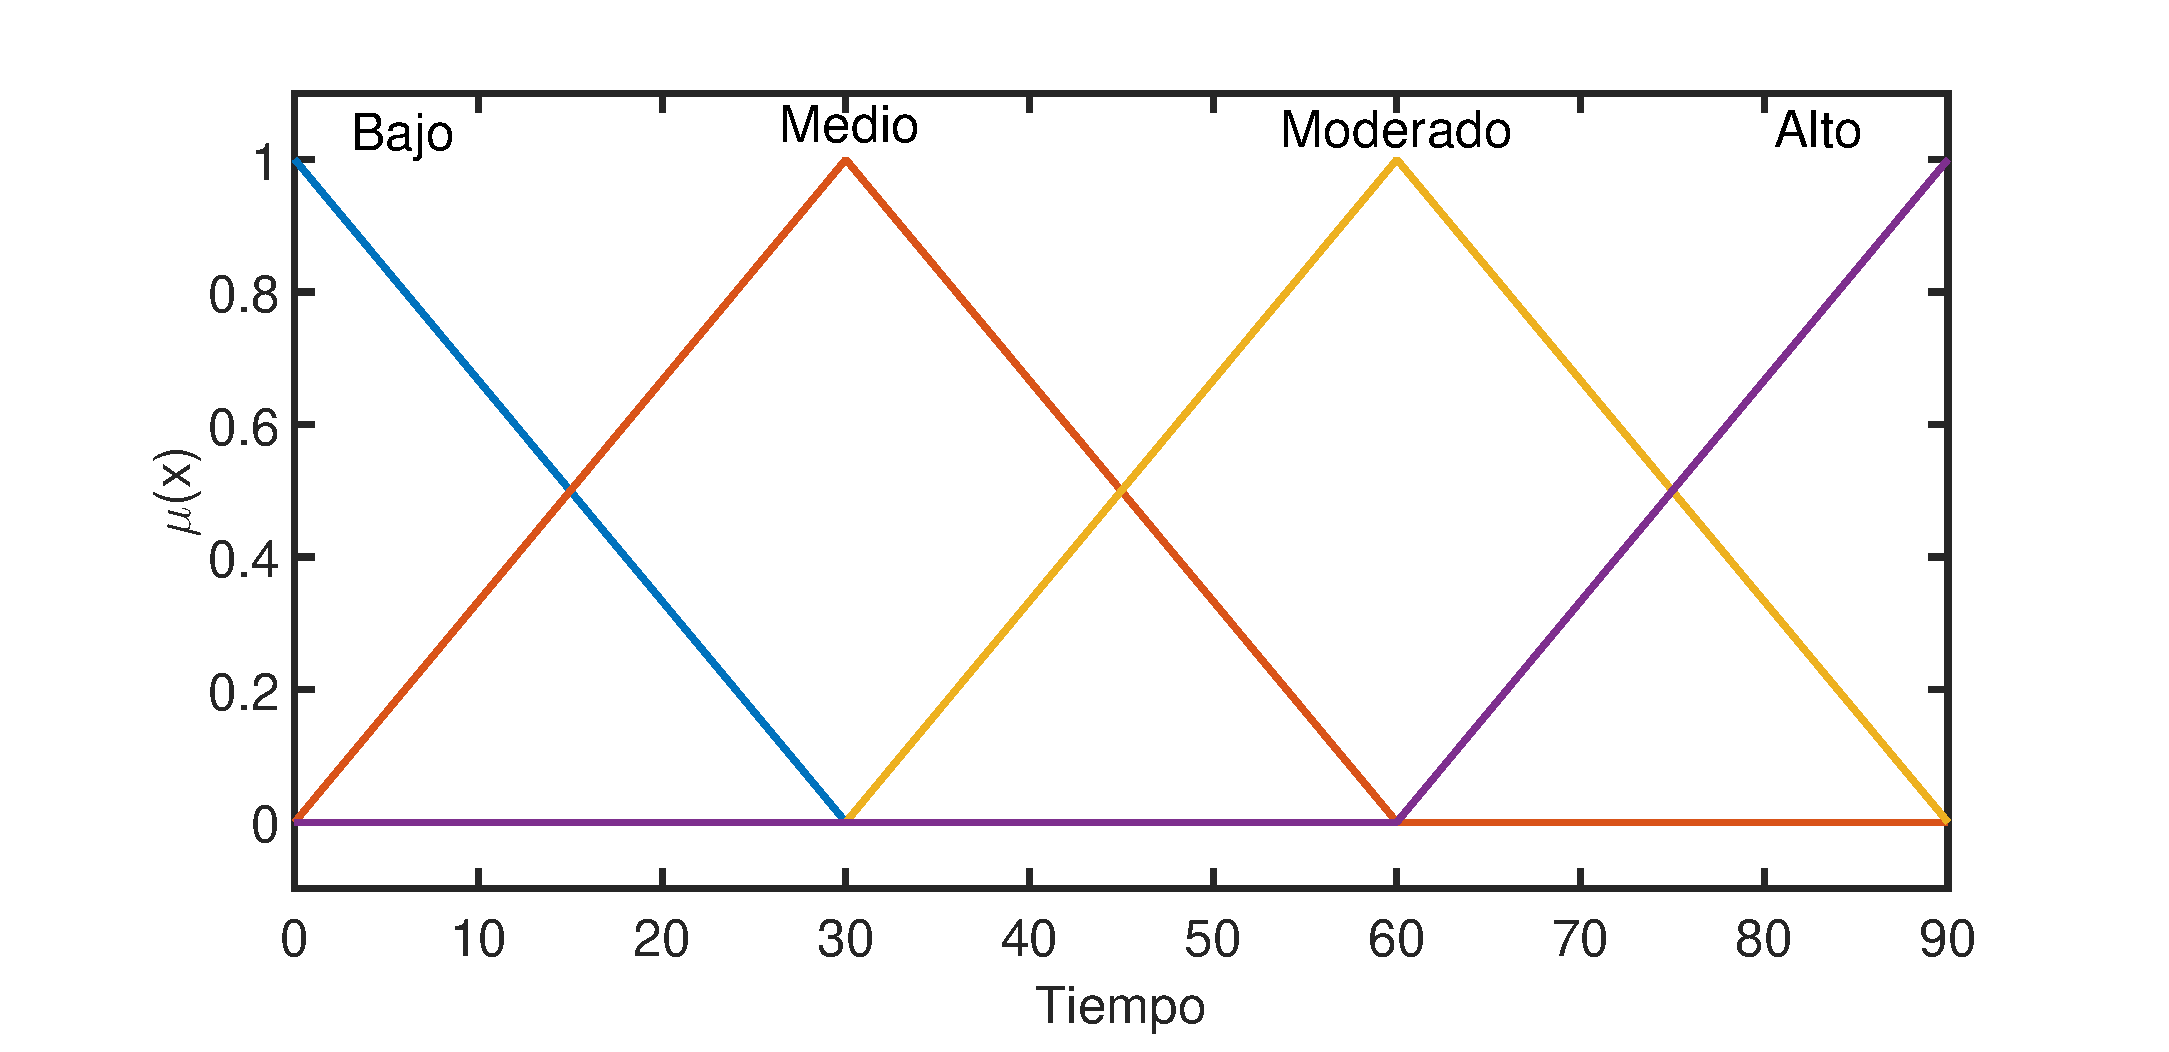
\includegraphics[height=5cm, width=12cm]{Variables/ConfigA_output1.eps}
	\caption[Gráfica variable lingüística tiempo - A]{Representación gráfica de la variable lingüística Tiempo}
\end{figure}

\subsubsection{Base de conocimientos}
La siguiente tabla muestra las reglas difusas empleadas en esta configuración.
\begin{longtable}[c]{lclcl} \toprule
	\multicolumn{3}{c}{Antecedente} & & Consecuente \\ \midrule
	Vehículos Pocos & Y & Congestión Baja& $\rightarrow$ & Verde Medio \\
	Vehículos Pocos & Y & Congestión Alta& $\rightarrow$ & Verde Bajo \\
	Vehículos Muchos &Y& Congestión Baja& $\rightarrow$ & Verde Alto \\
	Vehículos Muchos &Y& Congestión Alta& $\rightarrow$ & Verde Moderado \\ \hline
	\caption{Reglas difusas para la configuración \textit{A}}
\end{longtable}

\newpage
\subsubsection{Resultados}


Una vez diseñado e implementado el sistema de inferencia, se le suministraron valores de prueba para evaluar su desempeño. Los resultados de dicha evaluación se reflejan en la tabla siguiente:

\begin{table}[H]
	\centering
	\begin{tabular}{cccccc} \toprule
		$V \backslash C$ &  0 & 3 & 6 & 9 & 12 \\ \midrule
		0 & 30.00 & 28.99 & 26.21 & 20.86 & 09.70 \\
		3 & 39.02 & 39.03 & 37.69 & 35.58 & 33.96 \\
		6 & 46.40 & 45.83 & 45.00 & 44.16 & 43.59 \\
		9 & 56.03 & 54.41 & 52.30 & 50.96 & 50.97 \\
		12& 80.29 & 69.13 & 63.79 & 61.00 & 59.99 \\
		%\caption{Resultados de la evaluación para la configuración \textit{A}}
	\end{tabular}
	\caption{Resultados de la evaluación para la configuración}
\end{table}
Donde: la columna V son los valores de prueba de la variable Vehículos, la fila C son los valores de  prueba de la variable Congestión y las celdas son los tiempos (en segundos).




\subsubsection{Observaciones}
\begin{multicols}{2}

Después de evaluar el desempeño de la primera configuración se observa como efectivamente el tiempo asignado varía de acuerdo a las variables de entrada; sin embargo, el tiempo asignado para las entradas Vehículos = 0 y Congestión = 6, resulta excesivo puesto que la cantidad de vehículos a los que se les cederá el paso es mínimo (0) mientras que el índice de vehículos (6) que se mantendrán a la espera es bastante considerable.

\begin{figure}[H]
	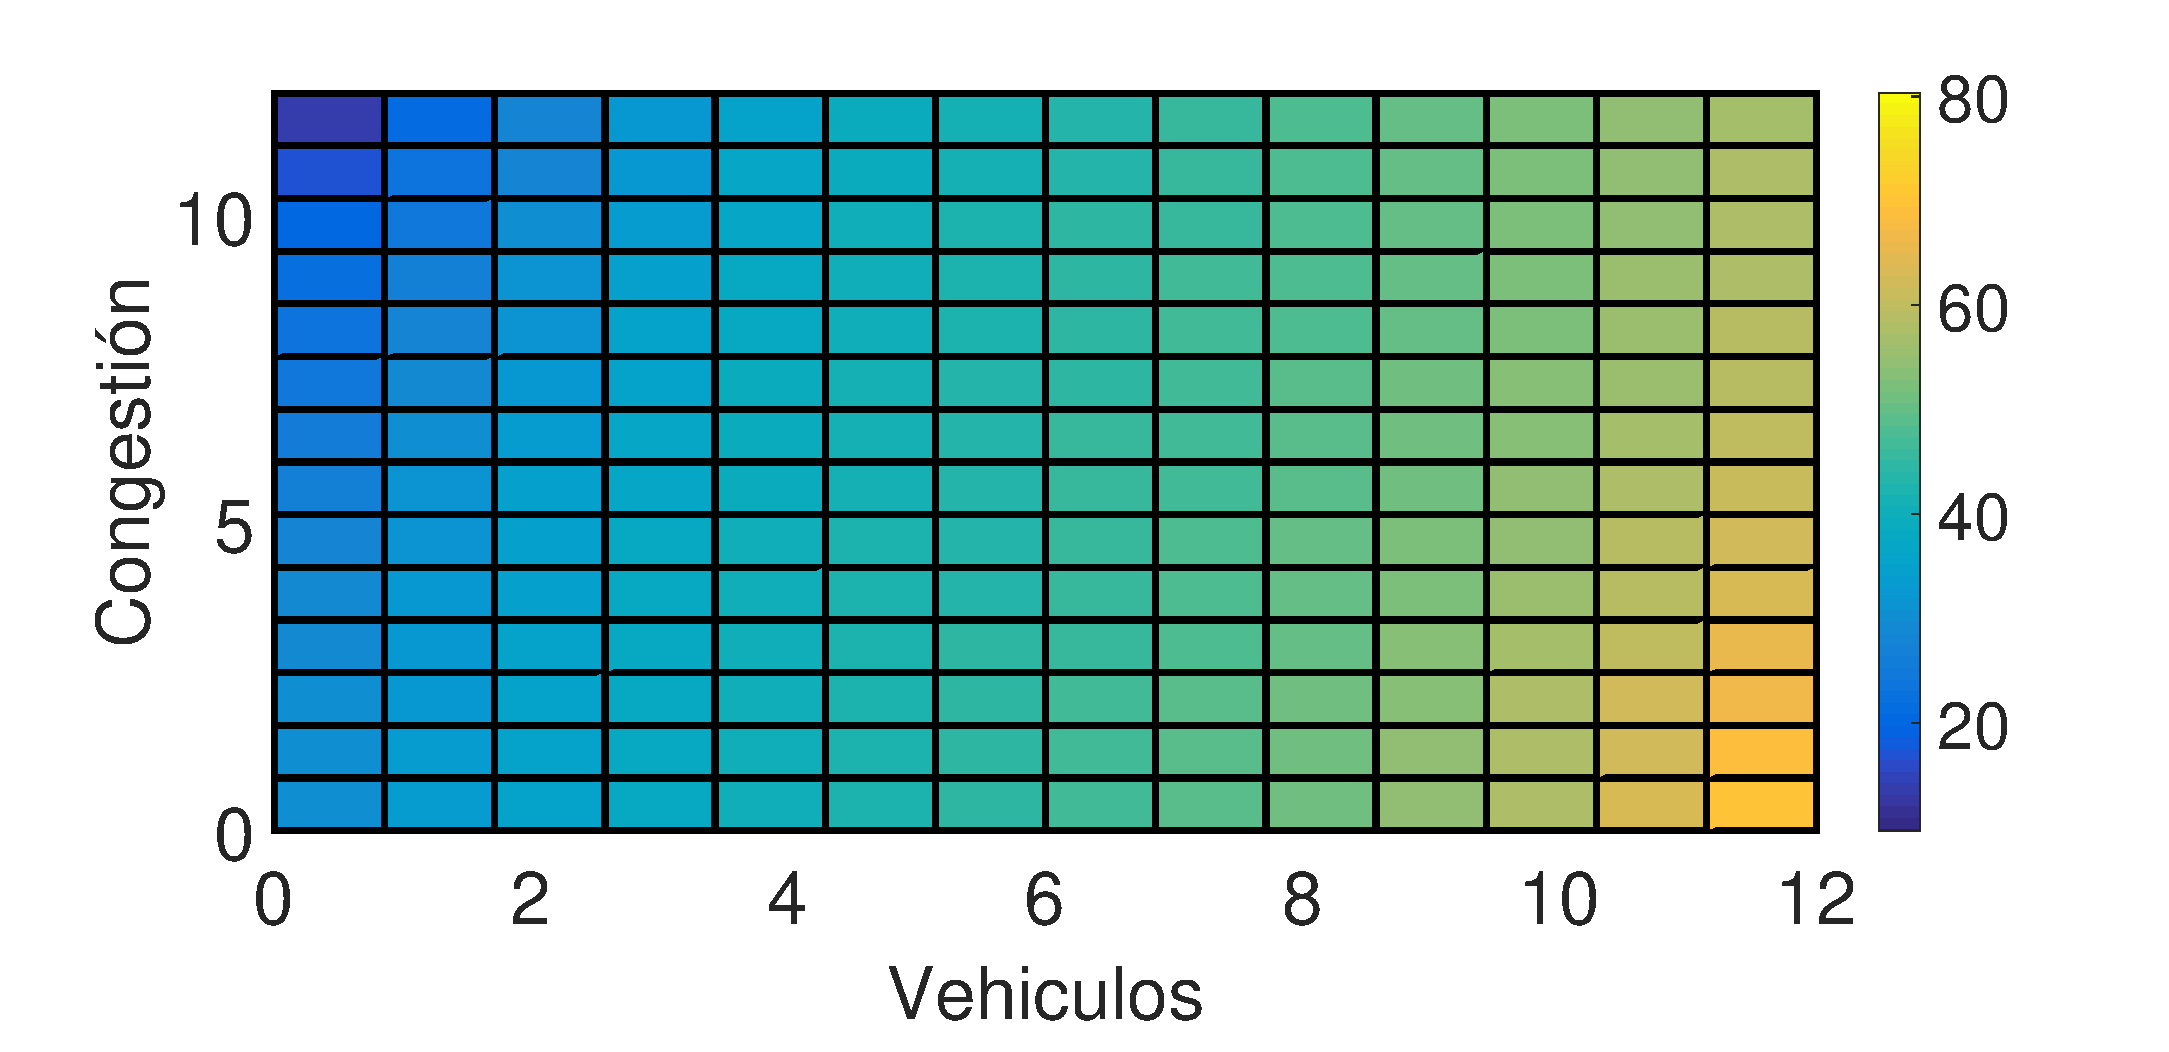
\includegraphics[width=0.5\textwidth]{Surfaces/Surface2D_A.eps}
	\caption{Superficie de control}
\end{figure}

\end{multicols}

 


\pagebreak
\subsection{Configuración B}
La configuración presentada en esta sección, ajusta los parámetros de las funciones de membresía de la variable de salida Tiempo. La configuración pasa a ser la siguiente: 

\textbf{Variable de entrada Vehículos.} Se mantiene sin cambios.

\begin{table}[!h]
	\centering
	\begin{tabular}{llr} \toprule
		Termino lingüístico & Función de membresía & Parámetros \\ \midrule
		Pocos & Triangular & [0, 0, 12 ] \\
		Muchos & Triangular & [0, 12, 12] \\ \bottomrule
	\end{tabular}
	\caption{Variable lingüística \textit{Vehículos}}
\end{table}


\textbf{Variable de entrada Congestión.} Se mantiene sin cambios desde la configuración anterior.


\begin{table}[!h]
	\centering
	\begin{tabular}{llr} \toprule
		Termino lingüístico & Función de membresía & Parámetros \\ \midrule
		Baja & Triangular & [0, 0, 12 ] \\
		Alta & Triangular & [0, 12, 12] \\ \bottomrule
	\end{tabular}
	\caption{Variable lingüística \textit{Congestión}}
\end{table}

\begin{figure}[H]
	\centering
	\subfigure[Variable lingüística Vehículos]{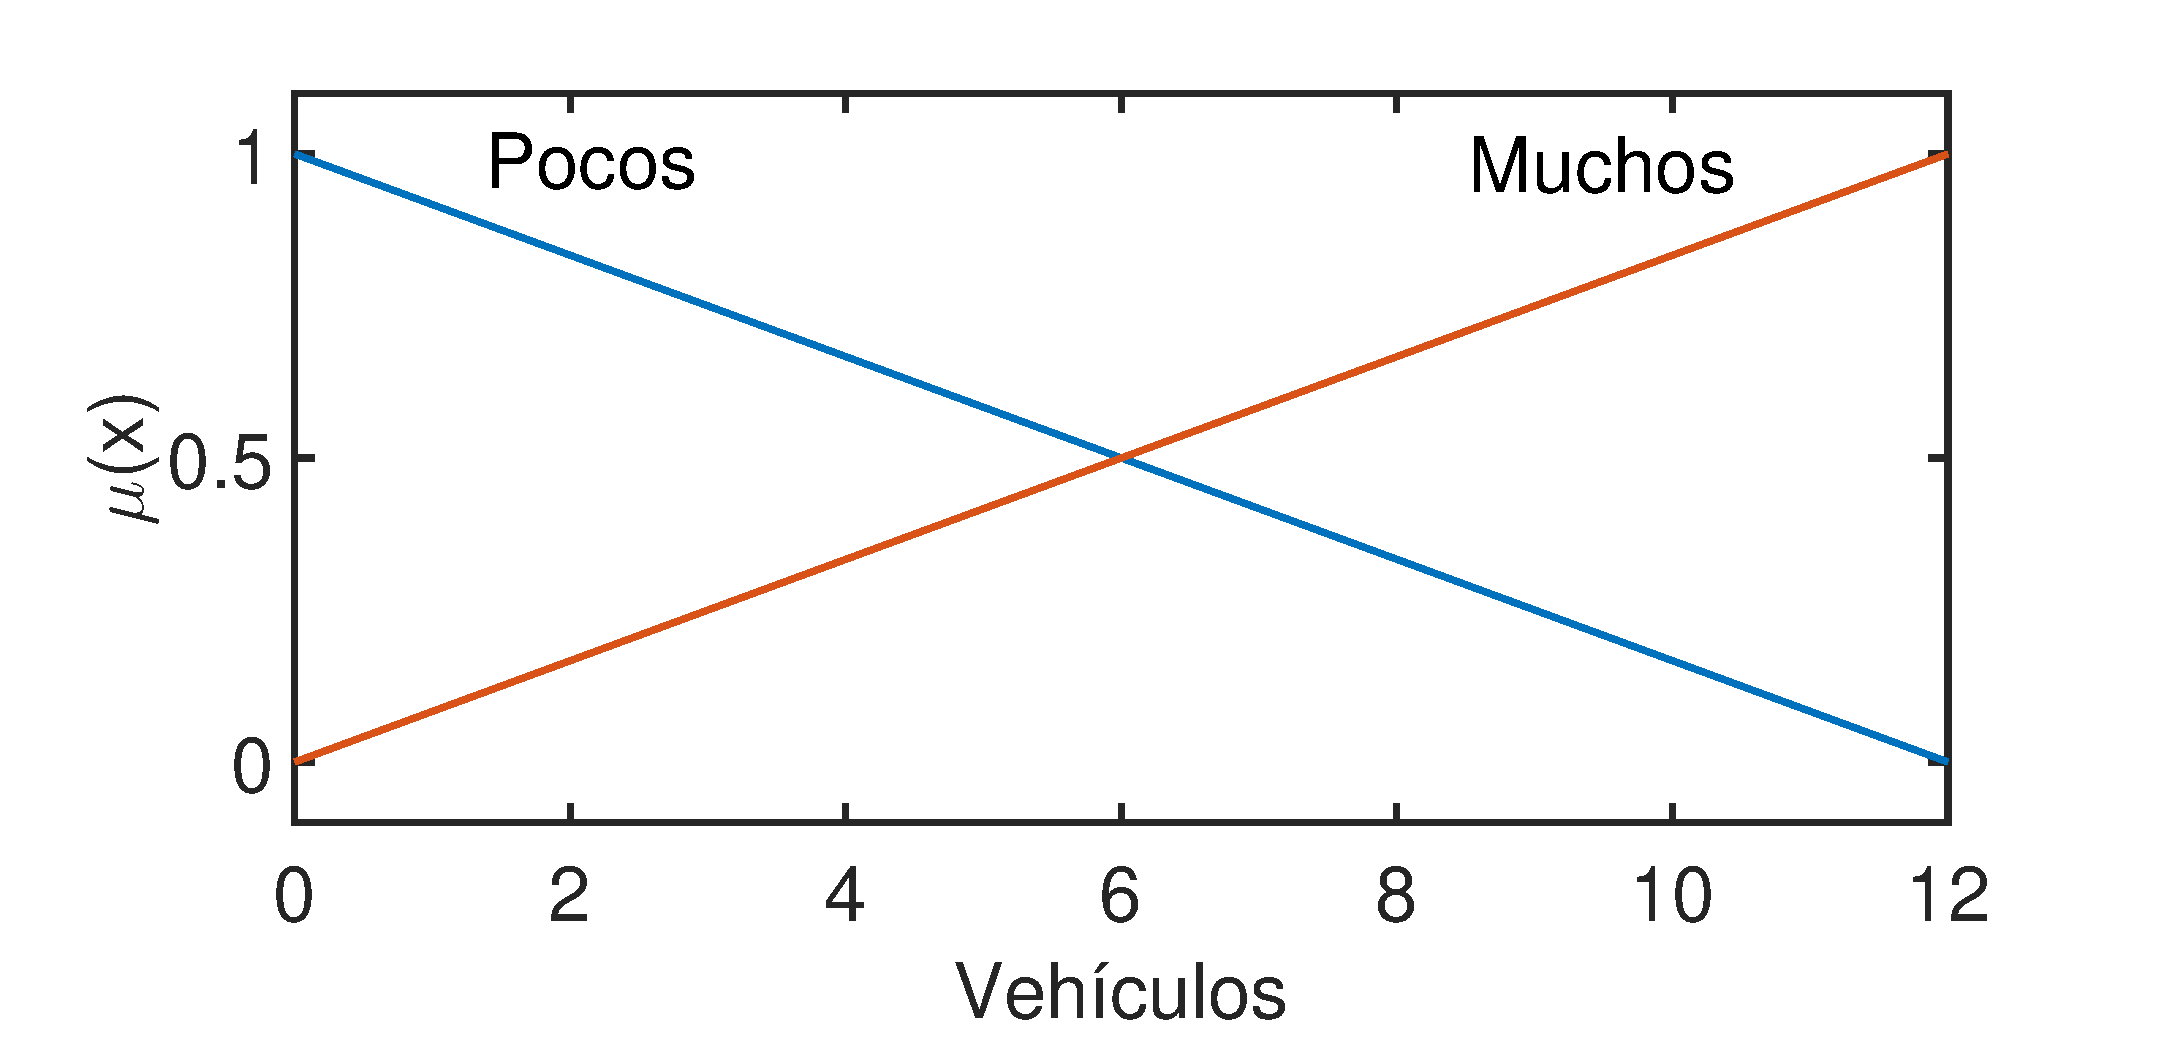
\includegraphics[height=4cm, width=8.1cm]{Variables/ConfigA_input1.eps}}
	\subfigure[Variable lingüística Congestión]{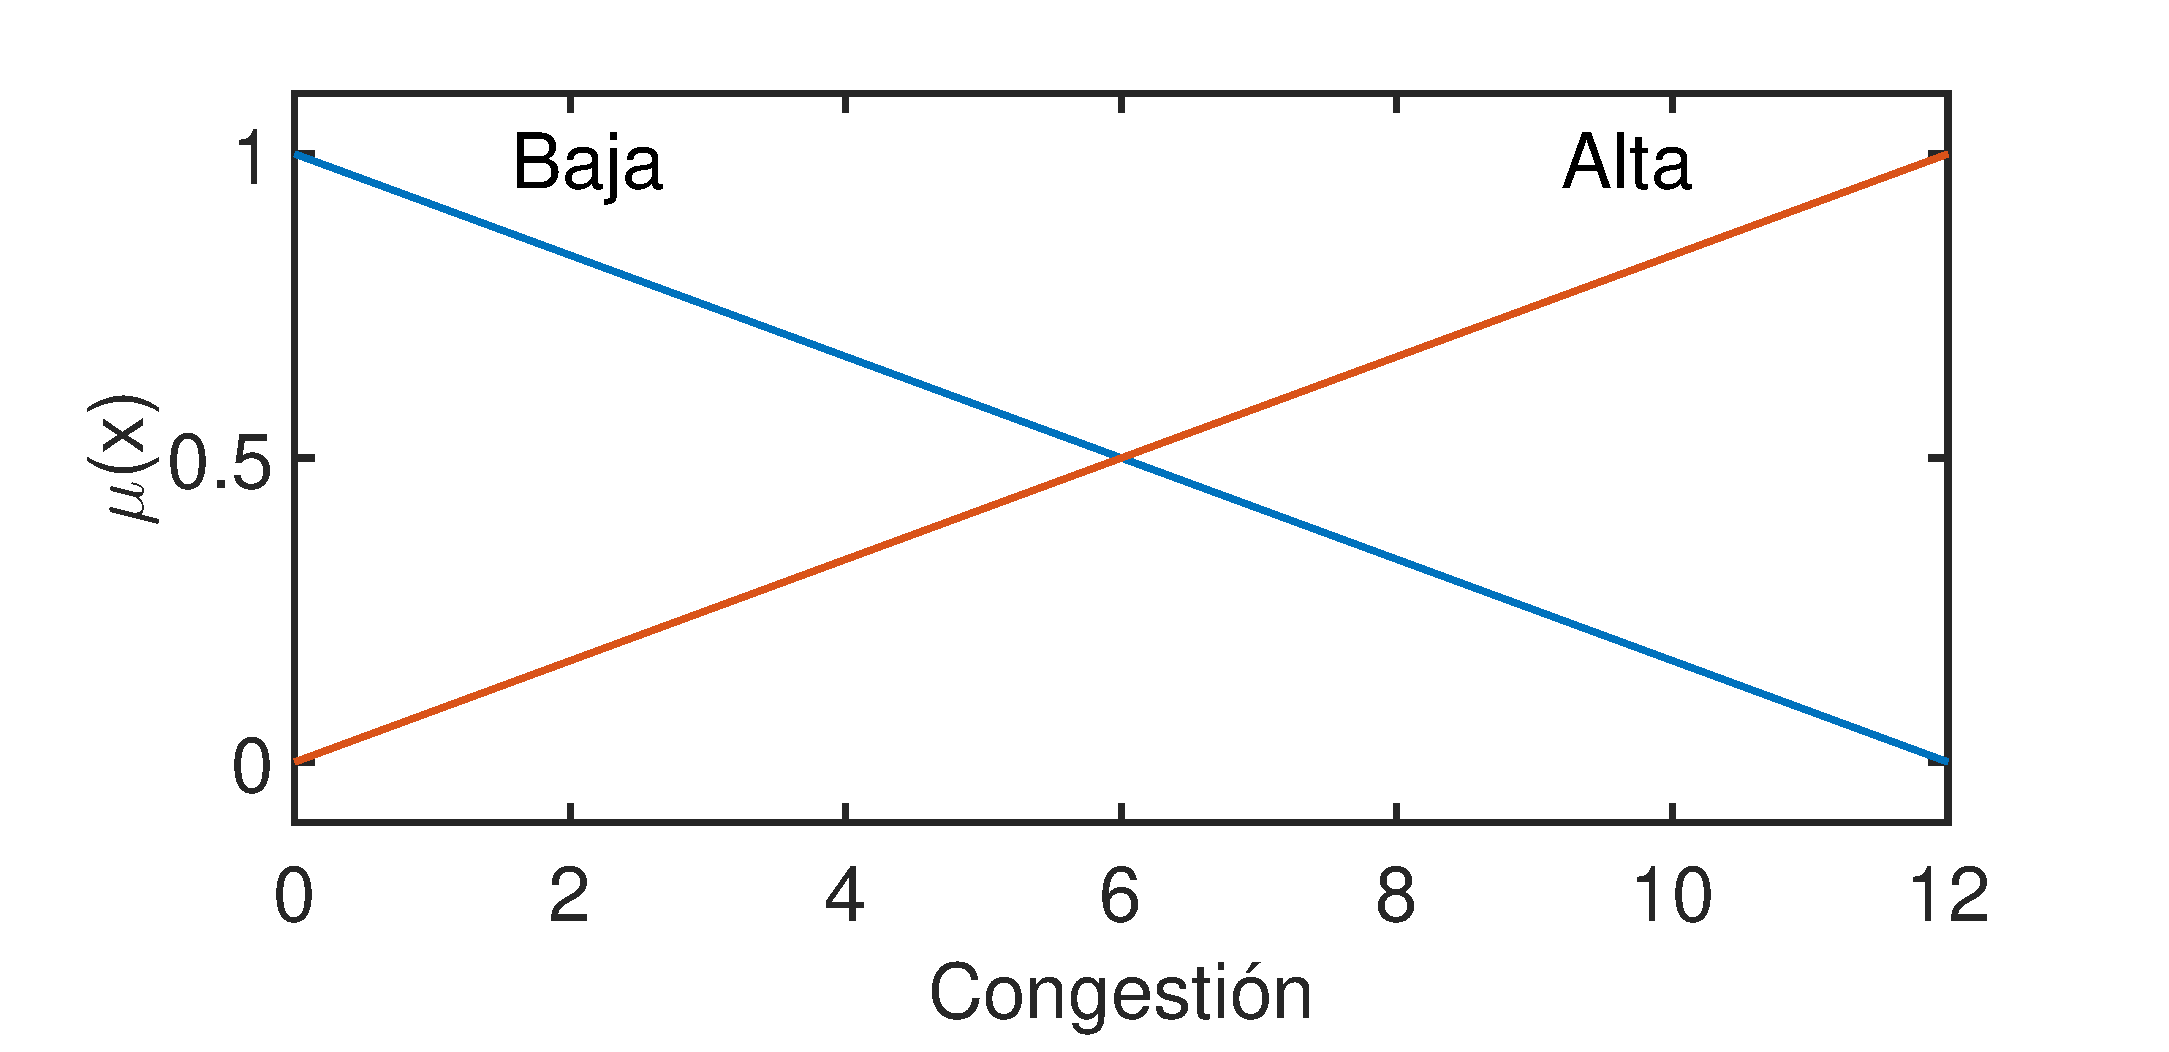
\includegraphics[height=4cm, width=8.1cm]{Variables/ConfigA_input2.eps}}
	\caption[Gráficas de las variables lingüísticas vehículos y congestión]{Representación gráfica de las variables lingüísticas Vehículos y Congestión }
\end{figure}

\pagebreak
\textbf{Variable de salida Tiempo.}
En esta ocasión los parámetros de las funciones de membresía fueron ajustados para generar tiempos más acertados. La nueva configuración de esta variable se muestra a continuación:


\begin{table}[!h]
	\centering
	\begin{tabular}{llr} \toprule
		Termino lingüístico & Función de membresía & Parámetros \\ \midrule
		Bajo & Triangular & [0, 0, 20 ] \\
		Medio & Triangular & [0, 20, 45] \\
		Moderado & Triangular & [20, 45, 70] \\
		Alto & Triangular & [45, 70, 70] \\ \bottomrule
	\end{tabular}
	\caption{Variable lingüística \textit{Tiempo}}
\end{table}

\begin{figure}[H]
	\centering
	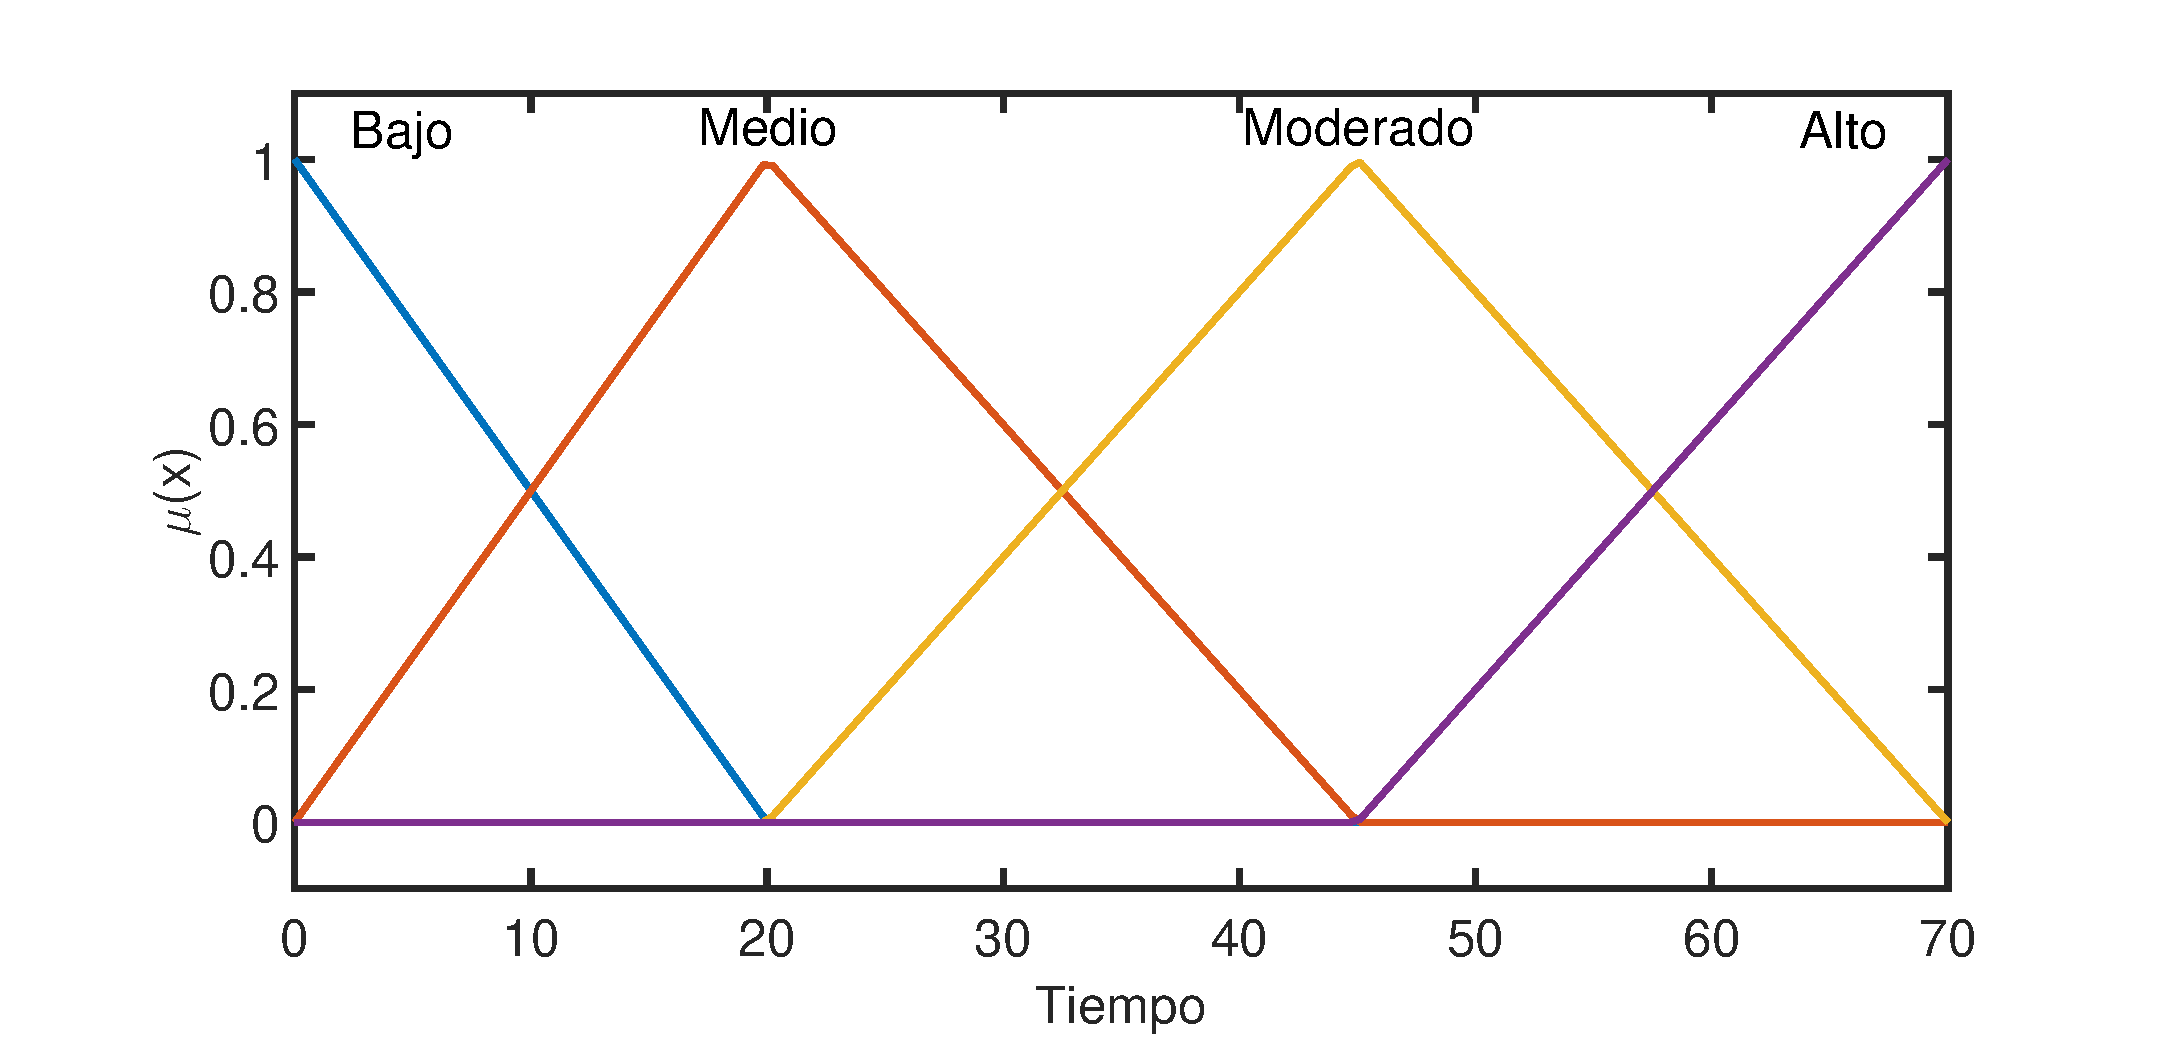
\includegraphics[height=5cm, width=12cm]{Variables/ConfigB_output1.eps}
	\caption[Gráfica variable lingüística tiempo - B]{Representación gráfica de la variable lingüística Tiempo}
\end{figure}

\subsubsection{Base de conocimientos}
La siguiente tabla muestra las reglas difusas empleadas en esta configuración que se mantiene sin cambios.
\begin{longtable}[c]{lclcl} \toprule
	\multicolumn{3}{c}{Antecedente} & & Consecuente \\ \midrule
	Vehículos Pocos & Y & Congestión Baja& $\rightarrow$ & Verde Medio \\
	Vehículos Pocos & Y & Congestión Alta& $\rightarrow$ & Verde Bajo \\
	Vehículos Muchos &Y& Congestión Baja& $\rightarrow$ & Verde Alto \\
	Vehículos Muchos &Y& Congestión Alta& $\rightarrow$ & Verde Moderado \\ \hline
	\caption{Reglas difusas para la configuración \textit{B}}
\end{longtable}

\pagebreak
\subsubsection{Resultados}
Una vez reajustados los parámetros del sistema de inferencia, se le suministraron lo mismos valores de prueba para evaluar su desempeño respecto a la configuración anterior. Los resultados de dicha evaluación se reflejan en la tabla siguiente:

\begin{longtable}[c]{cccccc} \toprule
	$V \backslash C$ &  0 & 3 & 6 & 9 & 12 \\ \midrule
	0 & 21.67 & 21.09 & 19.37 & 15.68 & 06.44 \\
	3 & 29.56 & 29.69 & 29.16 & 28.26 & 27.11 \\
	6 & 35.87 & 35.51 & 35.00 & 34.49 & 34.13 \\
	9 & 43.75 & 42.58 & 40.44 & 39.14 & 39.18 \\
	12& 61.90 & 52.60 & 48.15 & 45.83 & 45.00 \\
	\caption{Resultados de la evaluación para la configuración \textit{B}}
\end{longtable}

Donde: la columna V son los valores de prueba de la variable Vehículos, la fila C son los valores de  prueba de la variable Congestión y las celdas son los tiempos (en segundos) obtenidos por la configuración actual.

\subsubsection{Observaciones}
\begin{multicols}{2}
Después de evaluar el desempeño de la segunda configuración se observa como efectivamente el tiempo asignado es más acorde a la cantidad de vehículos; sin embargo, el tiempo asignado para las entradas Vehículos = 0 y Congestión = 0, resulta generoso puesto que la cantidad de vehículos a los que se les cederá el paso es mínimo (0) mientras al igual que el índice de vehículos (6); Sería mejor que en estos casos el tiempo fuera más corto para acelerar el ciclo del semáforo y reducir la espera de las otras avenidas. En otro casos como V = 12 y C = 12, el tiempo podría resultar insuficiente para desahogar el tráfico, por lo que se ajustará en la siguiente configuración.

\begin{figure}[H]
	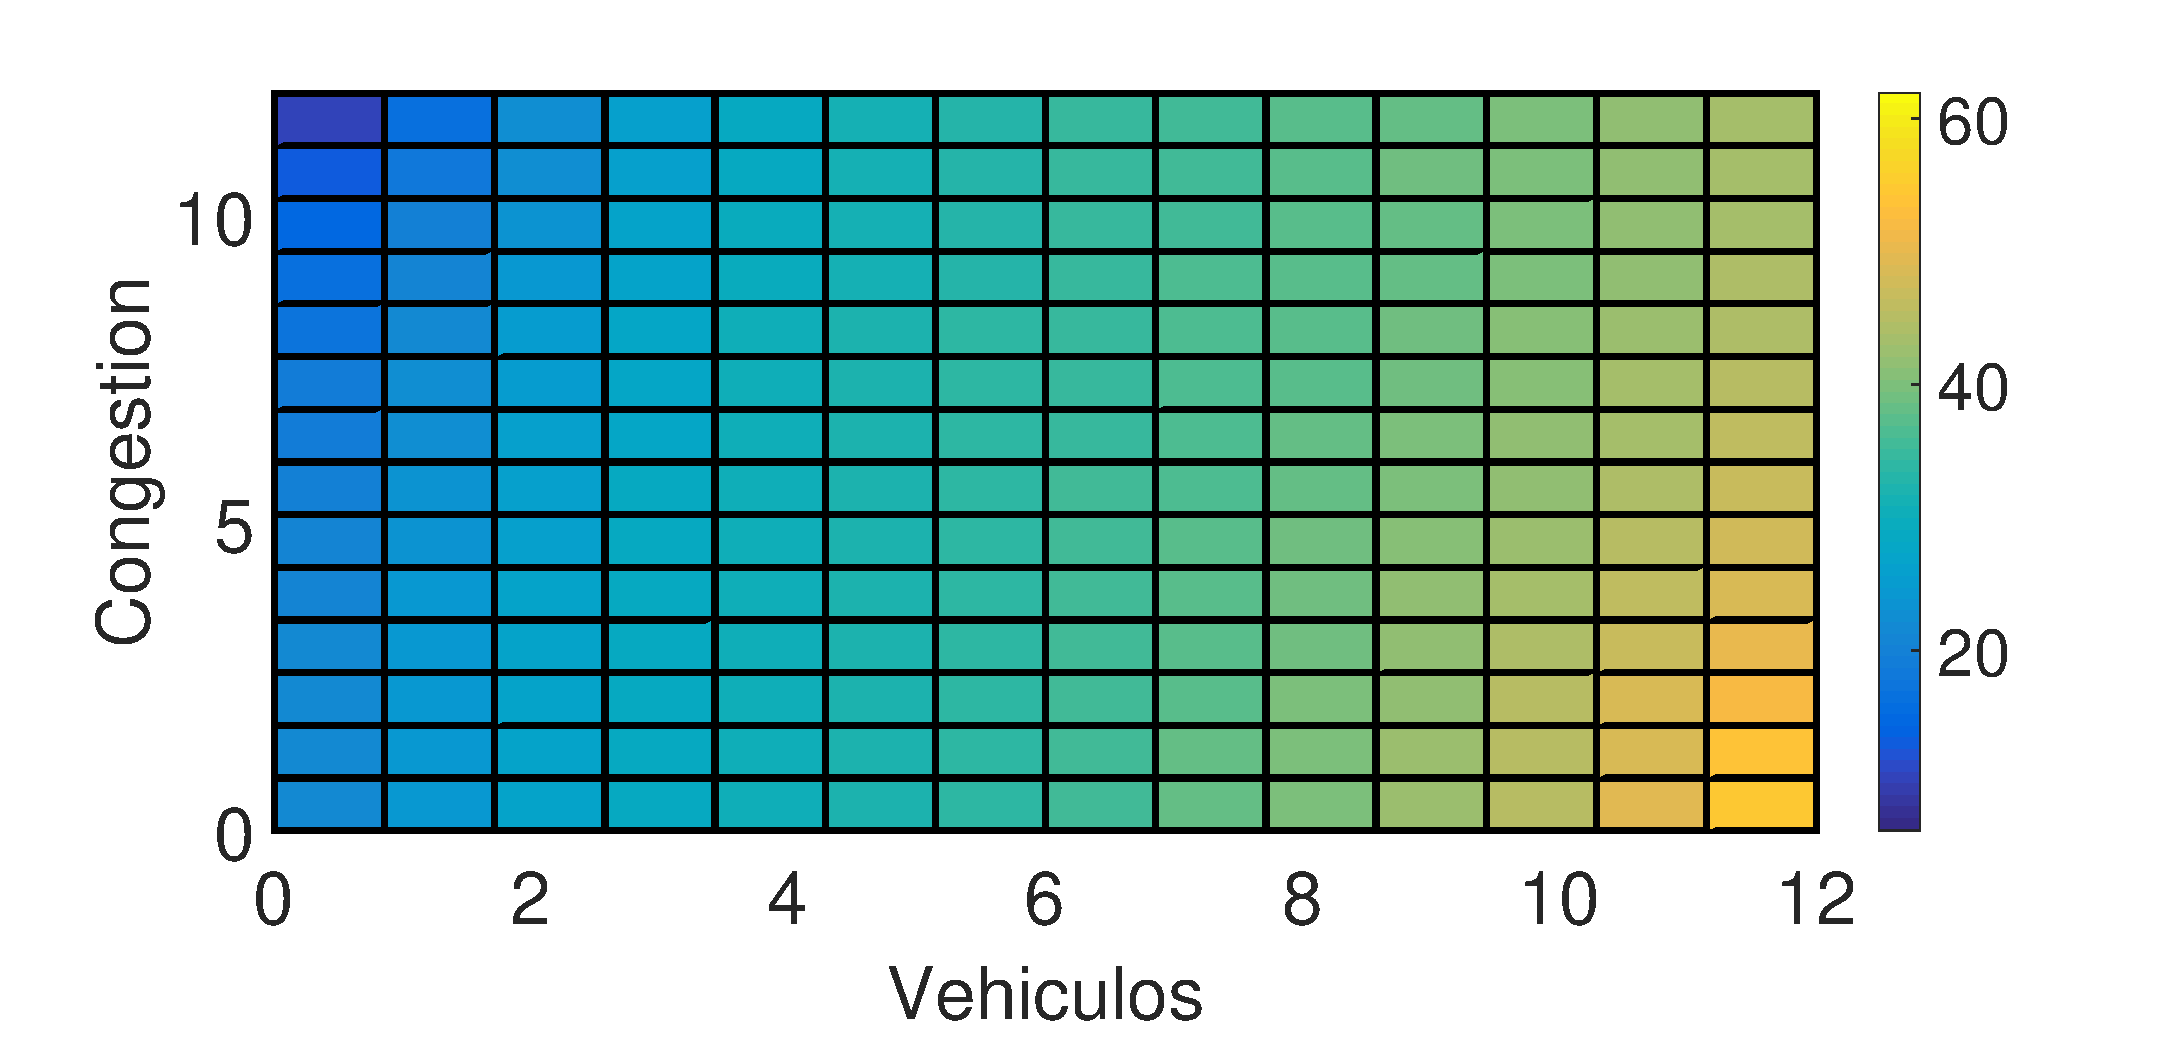
\includegraphics[width=0.5\textwidth]{Surfaces/Surface2D_B.eps}
	\caption{Superficie de control}
\end{figure}

\end{multicols}


\pagebreak
\subsection{Configuración C}
En está ocasión los reajustes serán mayores a los de la configuración anterior. Puesto que se agregaran un nuevo termino lingüístico a las variables Vehículos y Tiempo.

\textbf{Variable de entrada Vehículos.} Se agrega un nuevo término lingüístico para aumentar la flexibilidad del sistema.

\begin{table}[!h]
	\centering
	\begin{tabular}{llr} \toprule
		Termino lingüístico & Función de membresía & Parámetros \\ \midrule
		Pocos & Triangular & [0, 0, 6 ] \\
		Moderados & Triangular & [0, 6, 12 ] \\
		Muchos & Triangular & [6, 12, 12] \\ \bottomrule
	\end{tabular}
	\caption{Variable lingüística \textit{Vehículos}}
\end{table}


\textbf{Variable de entrada Congestión.} Se mantiene sin cambios desde la configuración anterior.


\begin{table}[!h]
	\centering
	\begin{tabular}{llr} \toprule
		Termino lingüístico & Función de membresía & Parámetros \\ \midrule
		Baja & Triangular & [0, 0, 12 ] \\
		Alta & Triangular & [0, 12, 12] \\ \bottomrule
	\end{tabular}
	\caption{Variable lingüística \textit{Congestión}}
\end{table}

\begin{figure}[H]
	\centering
	\subfigure[Variable lingüística Vehículos]{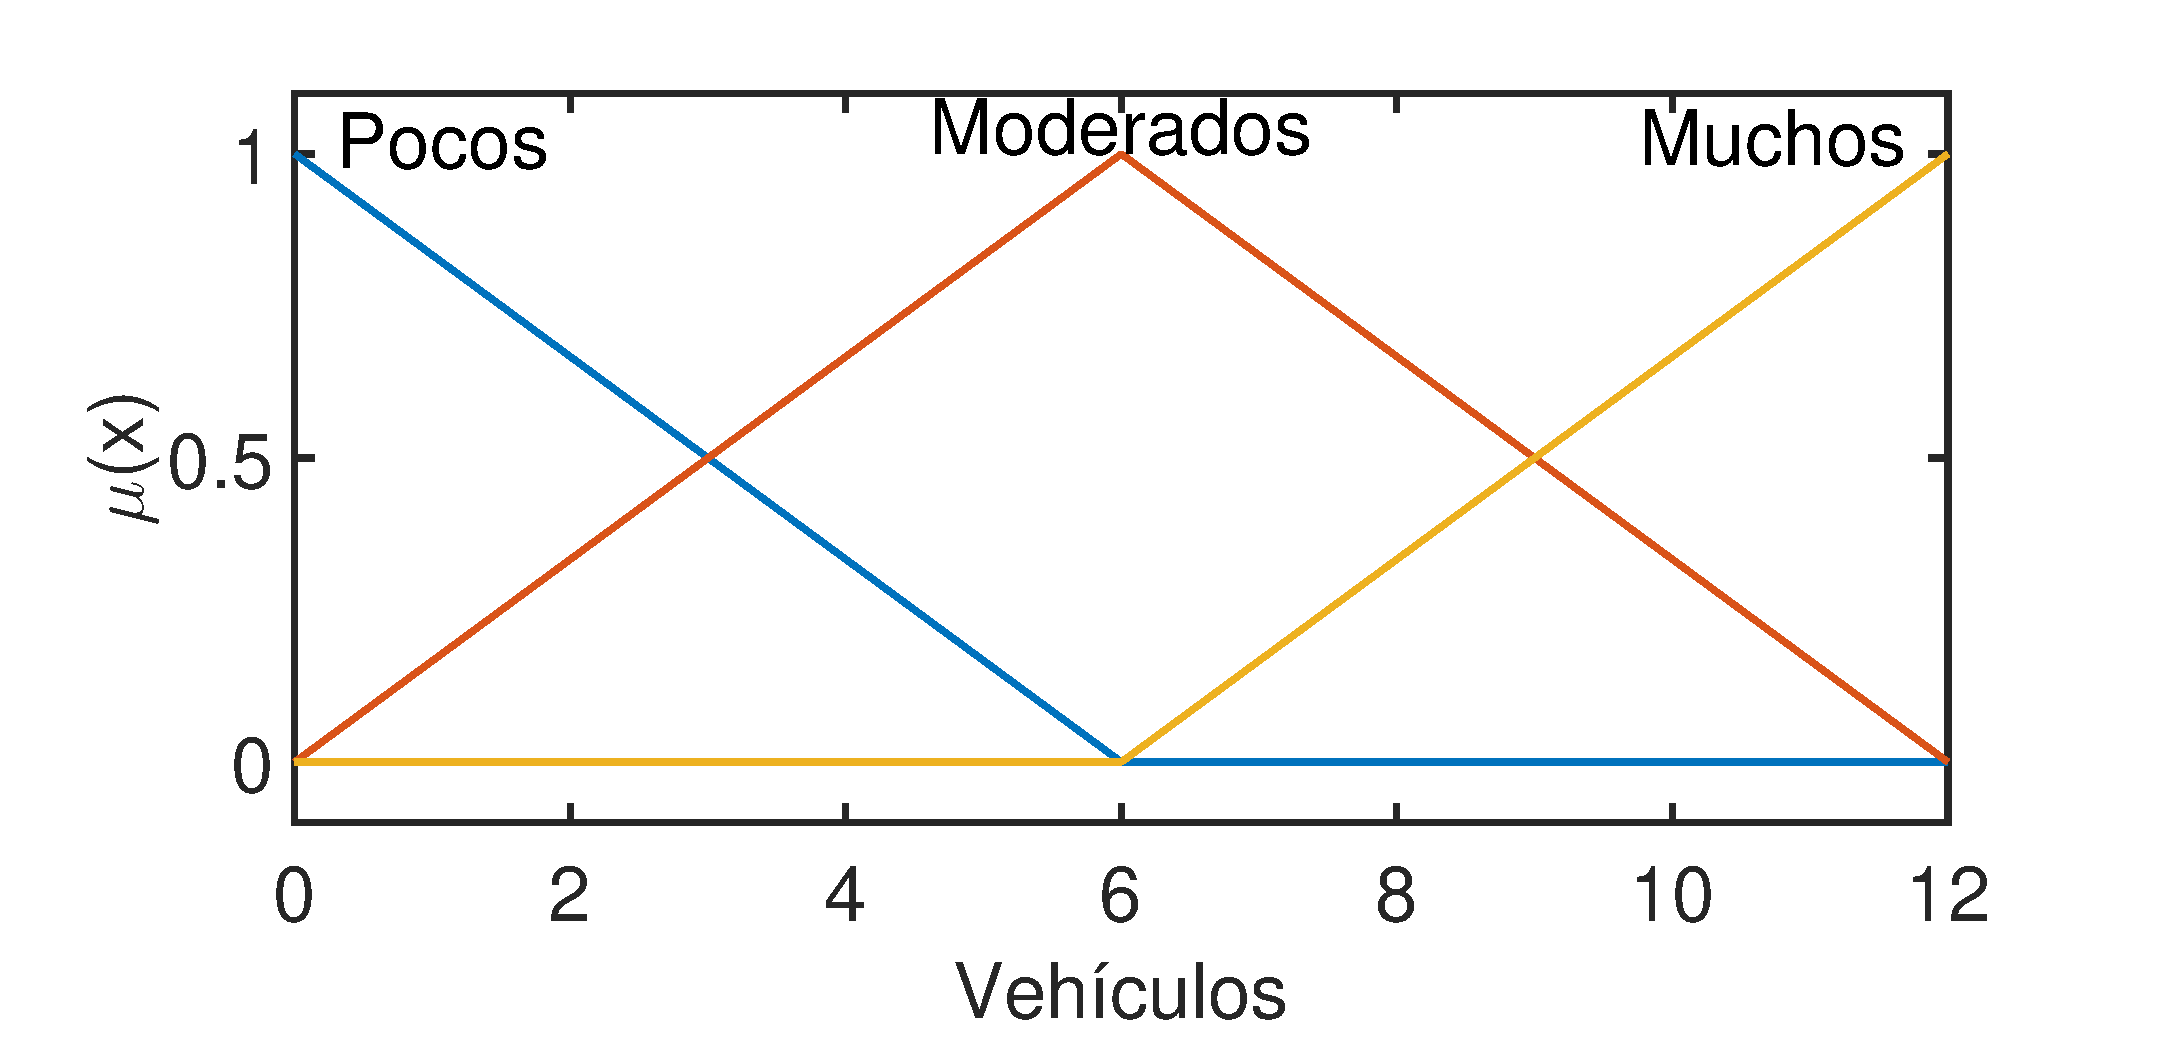
\includegraphics[height=4cm, width=8.1cm]{Variables/ConfigC_input1.eps}}
	\subfigure[Variable lingüística Congestión]{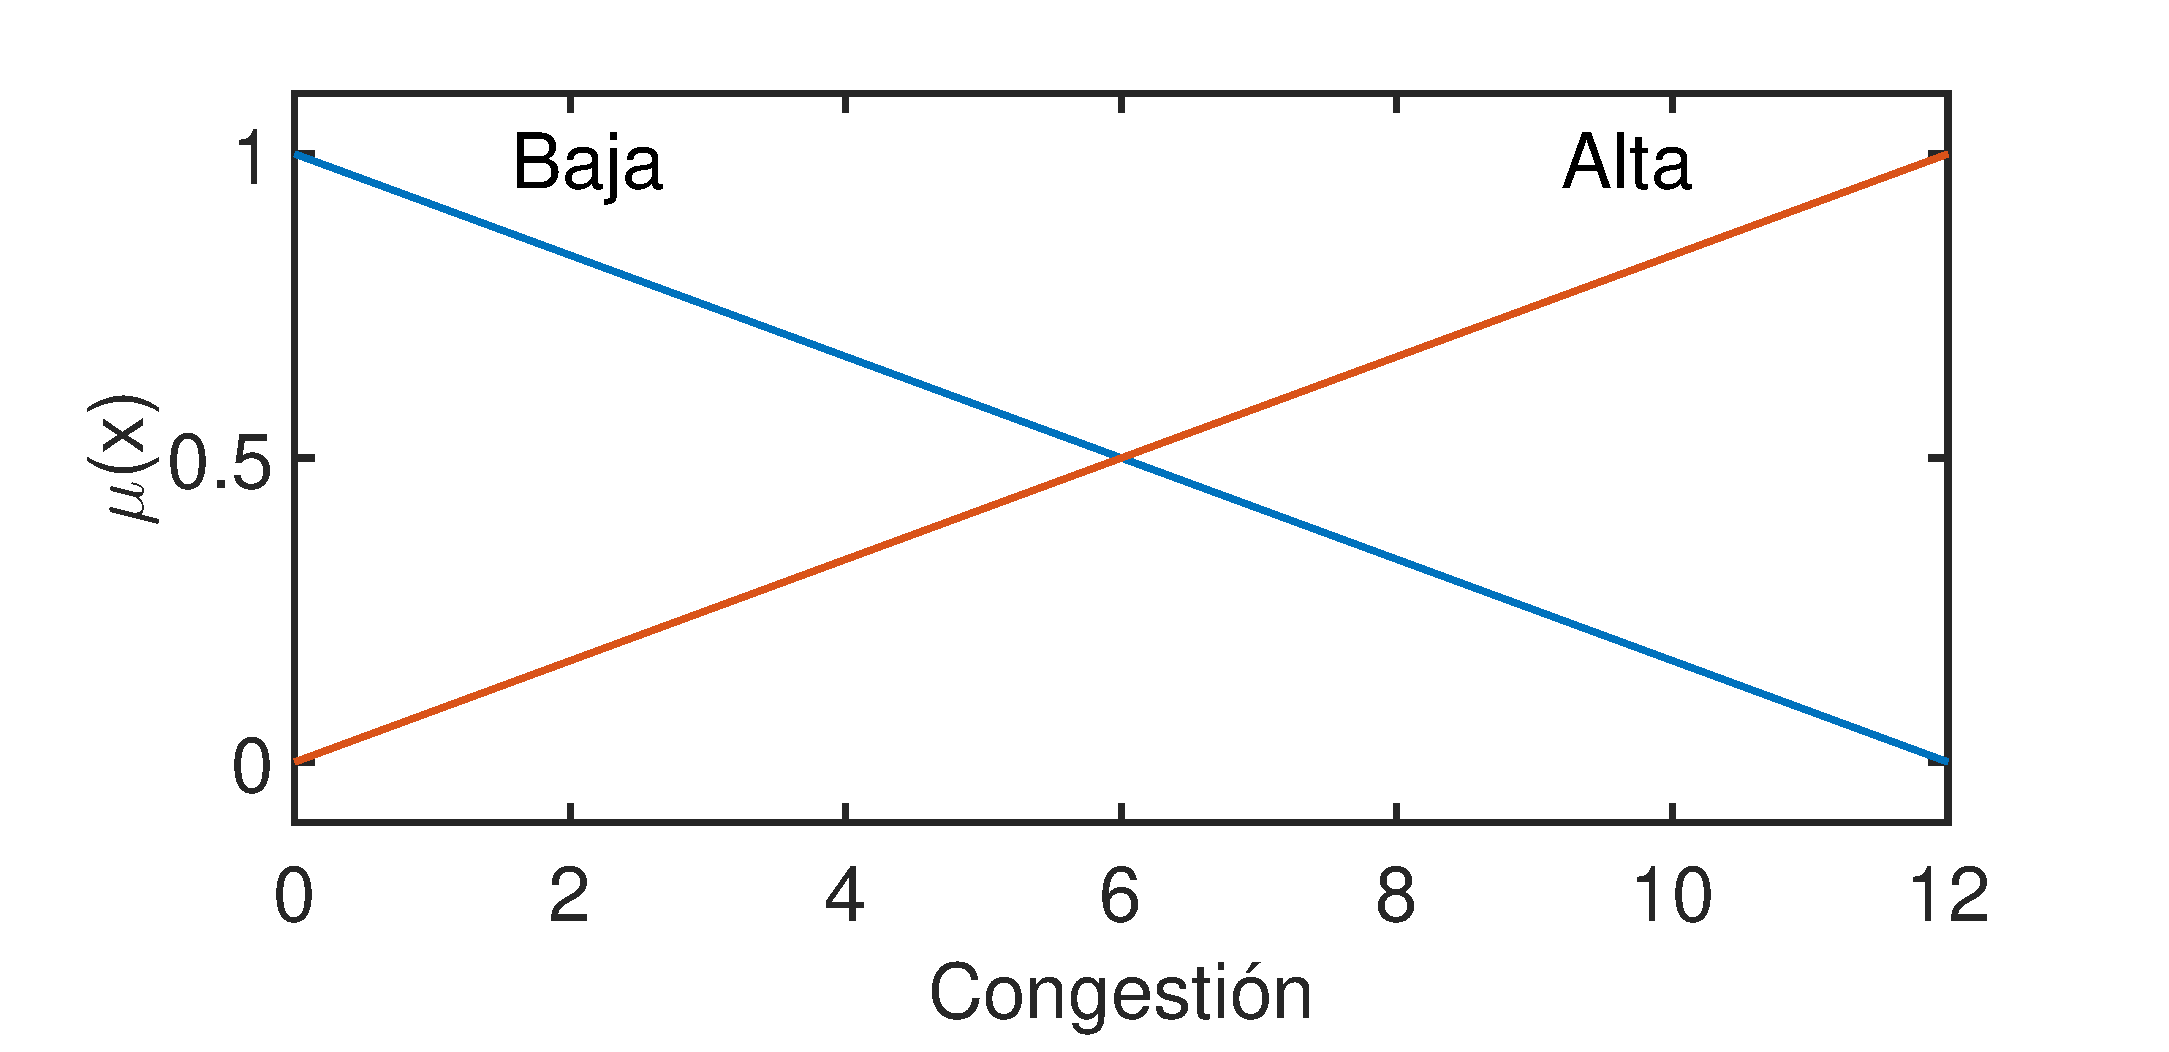
\includegraphics[height=4cm, width=8.1cm]{Variables/ConfigA_input2.eps}}
	\caption[Gráficas de las variables lingüísticas vehículos y congestión]{Representación gráfica de las variables lingüísticas Vehículos y Congestión }
\end{figure}

\pagebreak
\textbf{Variable de salida Tiempo.} Al igual que la variable vehículos, se ha agregado un nuevo término lingüístico para aumentar la flexibilidad. Además los parámetros de las funciones fueron reajustados ligeramente al igual que sus etiquetas.

\begin{table}[!h]
	\centering
	\begin{tabular}{llr} \toprule
		Termino lingüístico & Función de membresía & Parámetros \\ \midrule
		Mínimo & Triangular & [0, 10, 20 ] \\
		Bajo & Triangular & [0, 20, 40 ] \\
		Medio & Triangular & [20, 40, 60] \\
		Alto & Triangular & [40, 60, 80] \\
		Extra & Triangular & [60, 80, 80] \\ \bottomrule
	\end{tabular}
	\caption{Variable lingüística \textit{Tiempo}}
\end{table}

\begin{figure}[H]
	\centering
	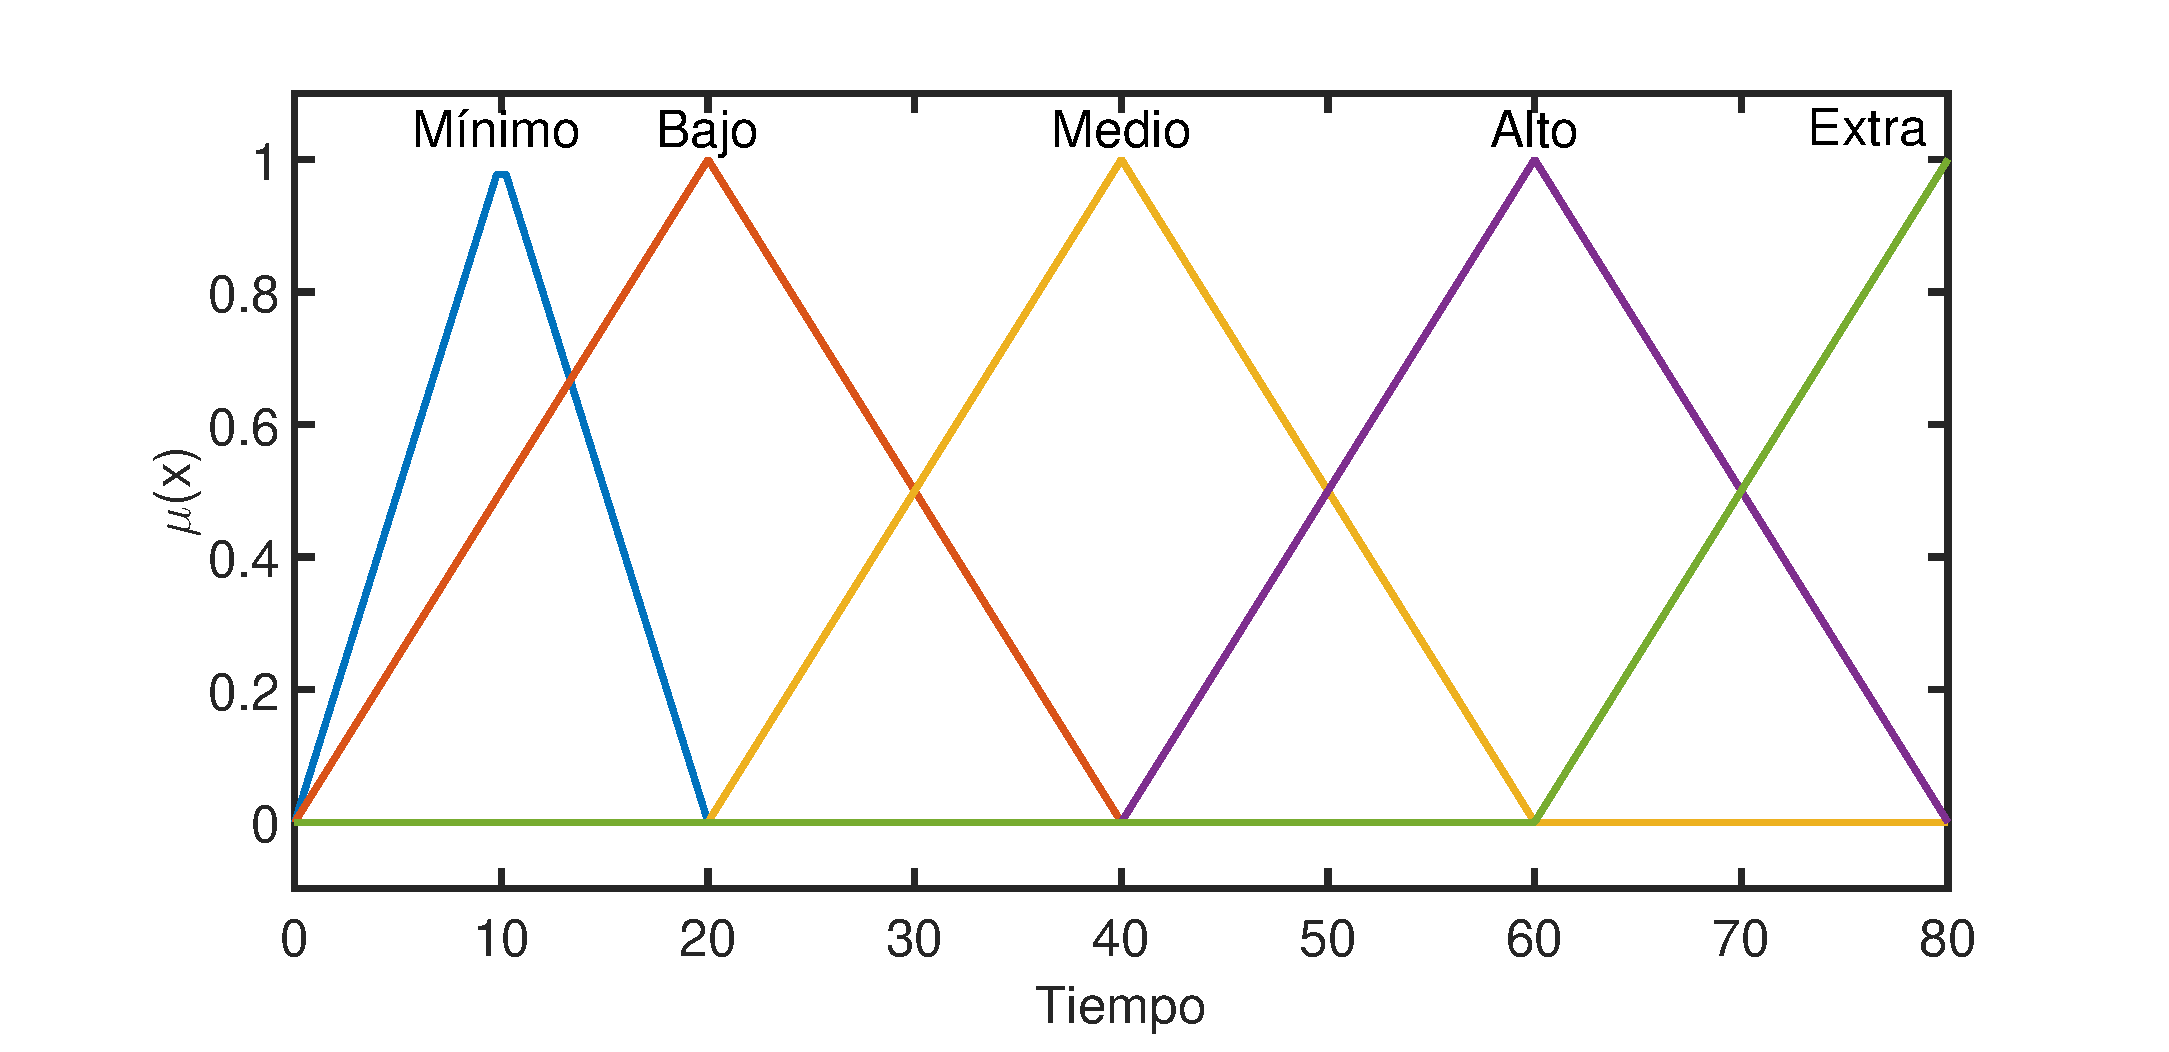
\includegraphics[height=5cm, width=12cm]{Variables/ConfigC_output1.eps}
	\caption[Gráfica variable lingüística tiempo - C]{Representación gráfica de la variable lingüística Tiempo}
\end{figure}

\subsubsection{Base de conocimientos}
La siguiente tabla muestra las reglas difusas empleadas en esta configuración que se mantiene sin cambios.
\begin{longtable}[c]{lclcl} \toprule
	\multicolumn{3}{c}{Antecedente} & & Consecuente \\ \midrule
	\multicolumn{3}{c}{Vehículos Pocos} & $\rightarrow$ & Verde Mínimo \\
	Vehículos Moderados & Y & Congestión Baja& $\rightarrow$ & Verde Medio \\
	Vehículos Moderados & Y & Congestión Alta& $\rightarrow$ & Verde Bajo \\
	Vehículos Muchos &Y& Congestión Baja& $\rightarrow$ & Verde Extra \\
	Vehículos Muchos &Y& Congestión Alta& $\rightarrow$ & Verde Alto \\ \hline
	\caption{Reglas difusas para la configuración \textit{C}}
\end{longtable}

\pagebreak
\subsubsection{Resultados}
Una vez reajustados los parámetros del sistema de inferencia, se le suministraron lo mismos valores de prueba para evaluar su desempeño respecto a la configuración anterior. Los resultados de dicha evaluación se reflejan en la tabla siguiente:

\begin{longtable}[c]{cccccc} \toprule
	$V \backslash C$ &  0 & 3 & 6 & 9 & 12 \\ \midrule
	0 & 10.00 & 10.00 & 10.00 & 10.00 & 10.00 \\
	3 & 30.00 & 29.63 & 28.81 & 25.59 & 18.85 \\
	6 & 40.00 & 34.21 & 30.00 & 25.79 & 20.00 \\
	9 & 59.74 & 44.49 & 42.44 & 40.75 & 40.00 \\
	12& 73.33 & 65.87 & 62.38 & 60.59 & 60.00 \\
	\caption{Resultados de la evaluación para la configuración \textit{C}}
\end{longtable}

Donde: la columna V son los valores de prueba de la variable Vehículos, la fila C son los valores de  prueba de la variable Congestión y las celdas son los tiempos (en segundos) obtenidos por la configuración actual.

\subsubsection{Observaciones}
\begin{multicols}{2}

	En esta tercera configuración se aprecia que hubo mejoras considerables en los tiempos inferidos por el sistema. Si se observa la salida para V = 12 y C = 12, cuya salida es 60, se nota que es un tiempo bastante acertado que ayudaría a desahogar la congestión. Por otro lado cuando V = 12 y C = 0, el sistema otorga 13 segundos extra. En el caso contrario, cuando V = 0 y C = 12, el sistema asigna el tiempo mínimo de 10 segundos. Hace falta un nuevo ajuste para saber si los tiempos pueden mejorar aún más.
	
	\begin{figure}[H]
		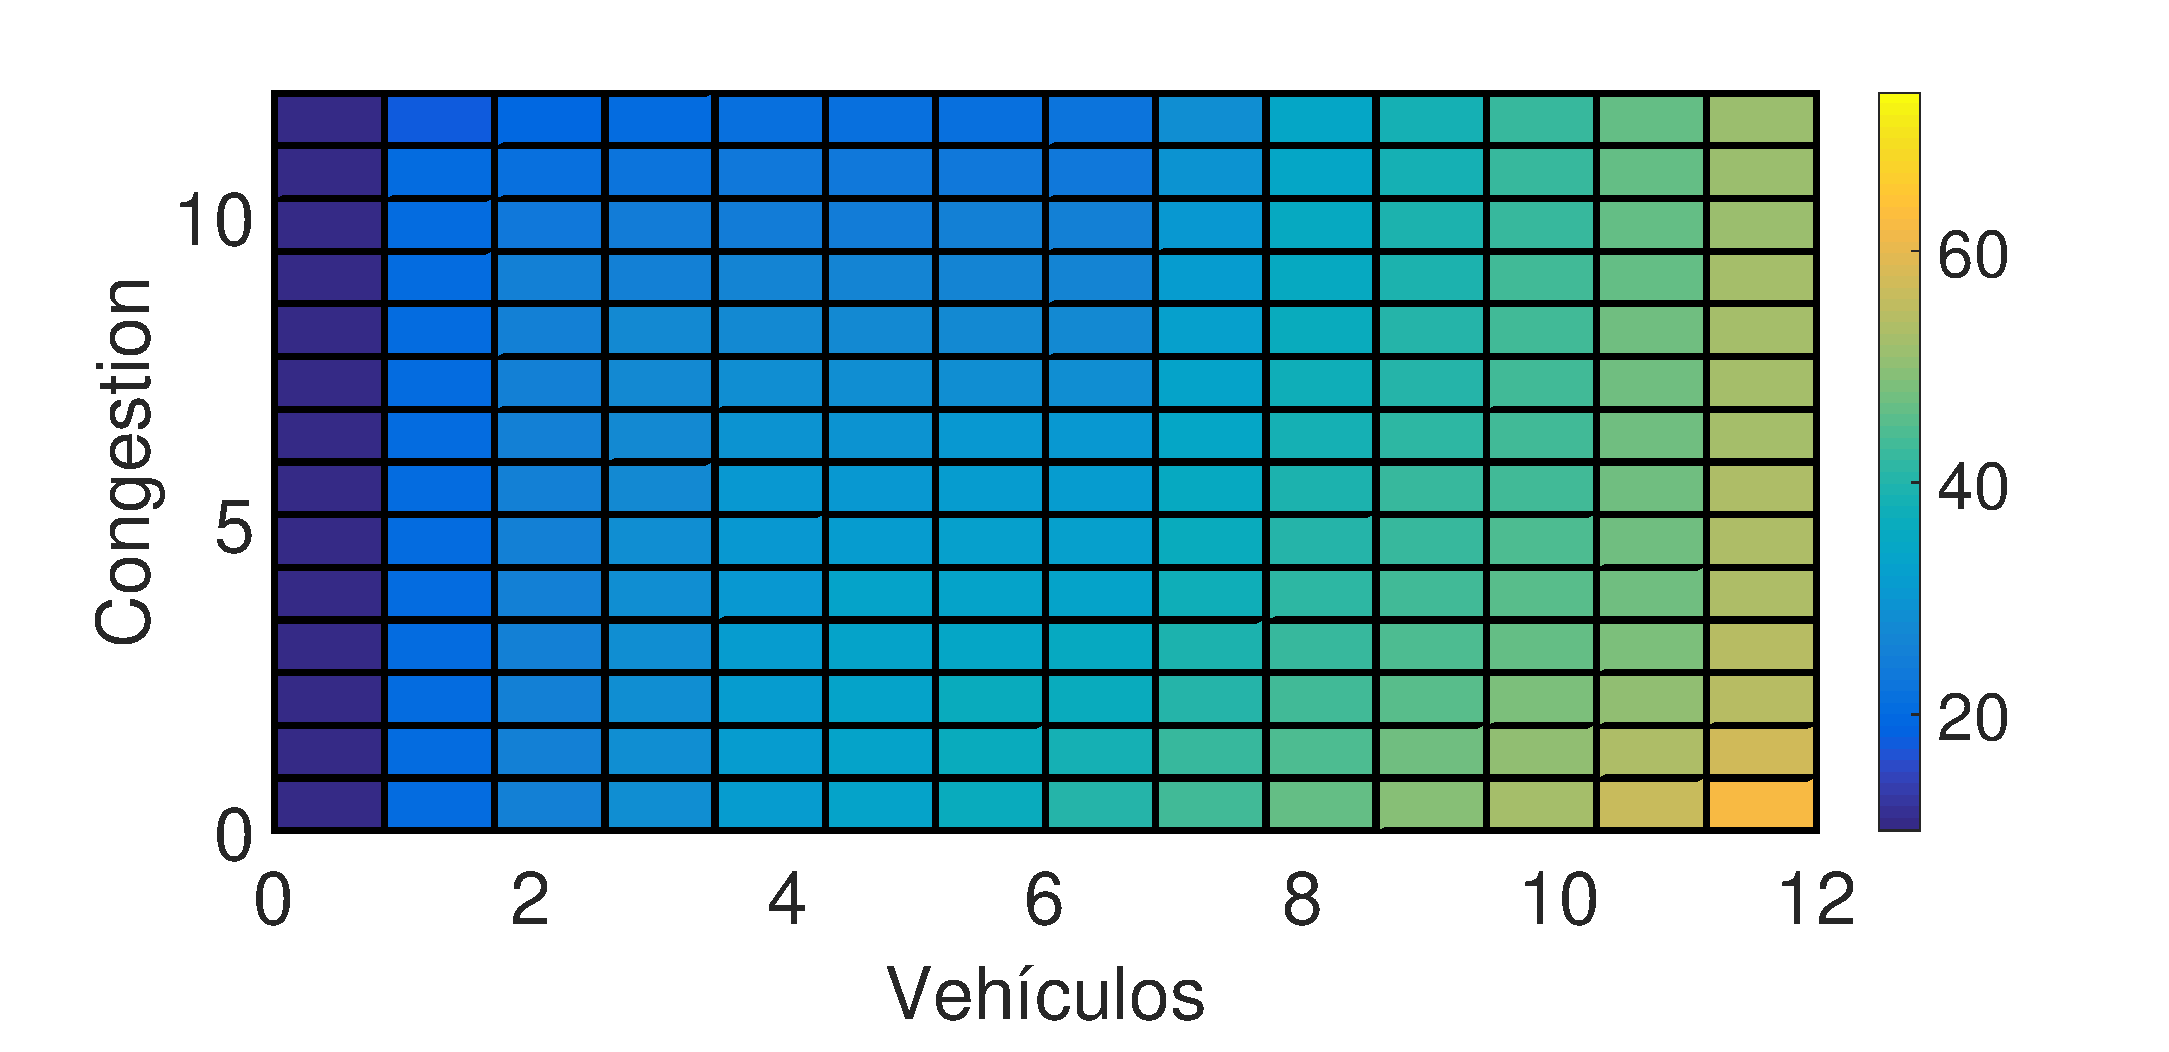
\includegraphics[width=0.5\textwidth]{Surfaces/Surface2D_C.eps}
		\caption{Superficie de control}
	\end{figure}
\end{multicols}
\pagebreak





\subsection{Configuración D}\label{section:configd}
Existen funciones de membresía que modelan mejor el modo de clasificación que realiza la mente humana, estas funciones son las curvas tales como: \textit{Sigmoidales, Gaussianas y Campanas Generalizadas}; en esta configuración se explota el potencial de las primeras dos.

\textbf{Variable de entrada Vehículos.} Las funciones de membresía \textit{triangulares} se remplazan por funciones \textit{Sigmoidales y Gaussianas}, estás modelan de manera más eficiente la manera en que el ser humano suele clasificar los fenómenos.
\begin{center}
	\begin{tabular}{llr} \toprule
		Termino lingüístico & Función de membresía & Parámetros \\ \midrule
		Pocos & Sigmoidal & [ -0.8, 4 ] \\
		Moderados & Gaussiana & [ 1.6, 7 ] \\
		Muchos & Sigmoidal & [ 0.8, 10] \\ \bottomrule
	\end{tabular}
	\captionof{table}{Variable lingüística \textit{Vehículos}}
\end{center}

\textbf{Variable de entrada Congestión.} También se remplaza las funciones triangulares por \textit{funciones Sigmoidales}.

\begin{table}[!h]
	\centering
	\begin{tabular}{llr} \toprule
		Termino lingüístico & Función de membresía & Parámetros \\ \midrule
		Baja & Sigmoidal & [ -0.8, 5 ] \\
		Alta & Sigmoidal & [ 0.8, 5 ] \\ \bottomrule
	\end{tabular}
	\caption{Variable lingüística \textit{Congestión}}
\end{table}
\begin{figure}[H]
	\centering
	\subfigure[Variable lingüística Vehículos]{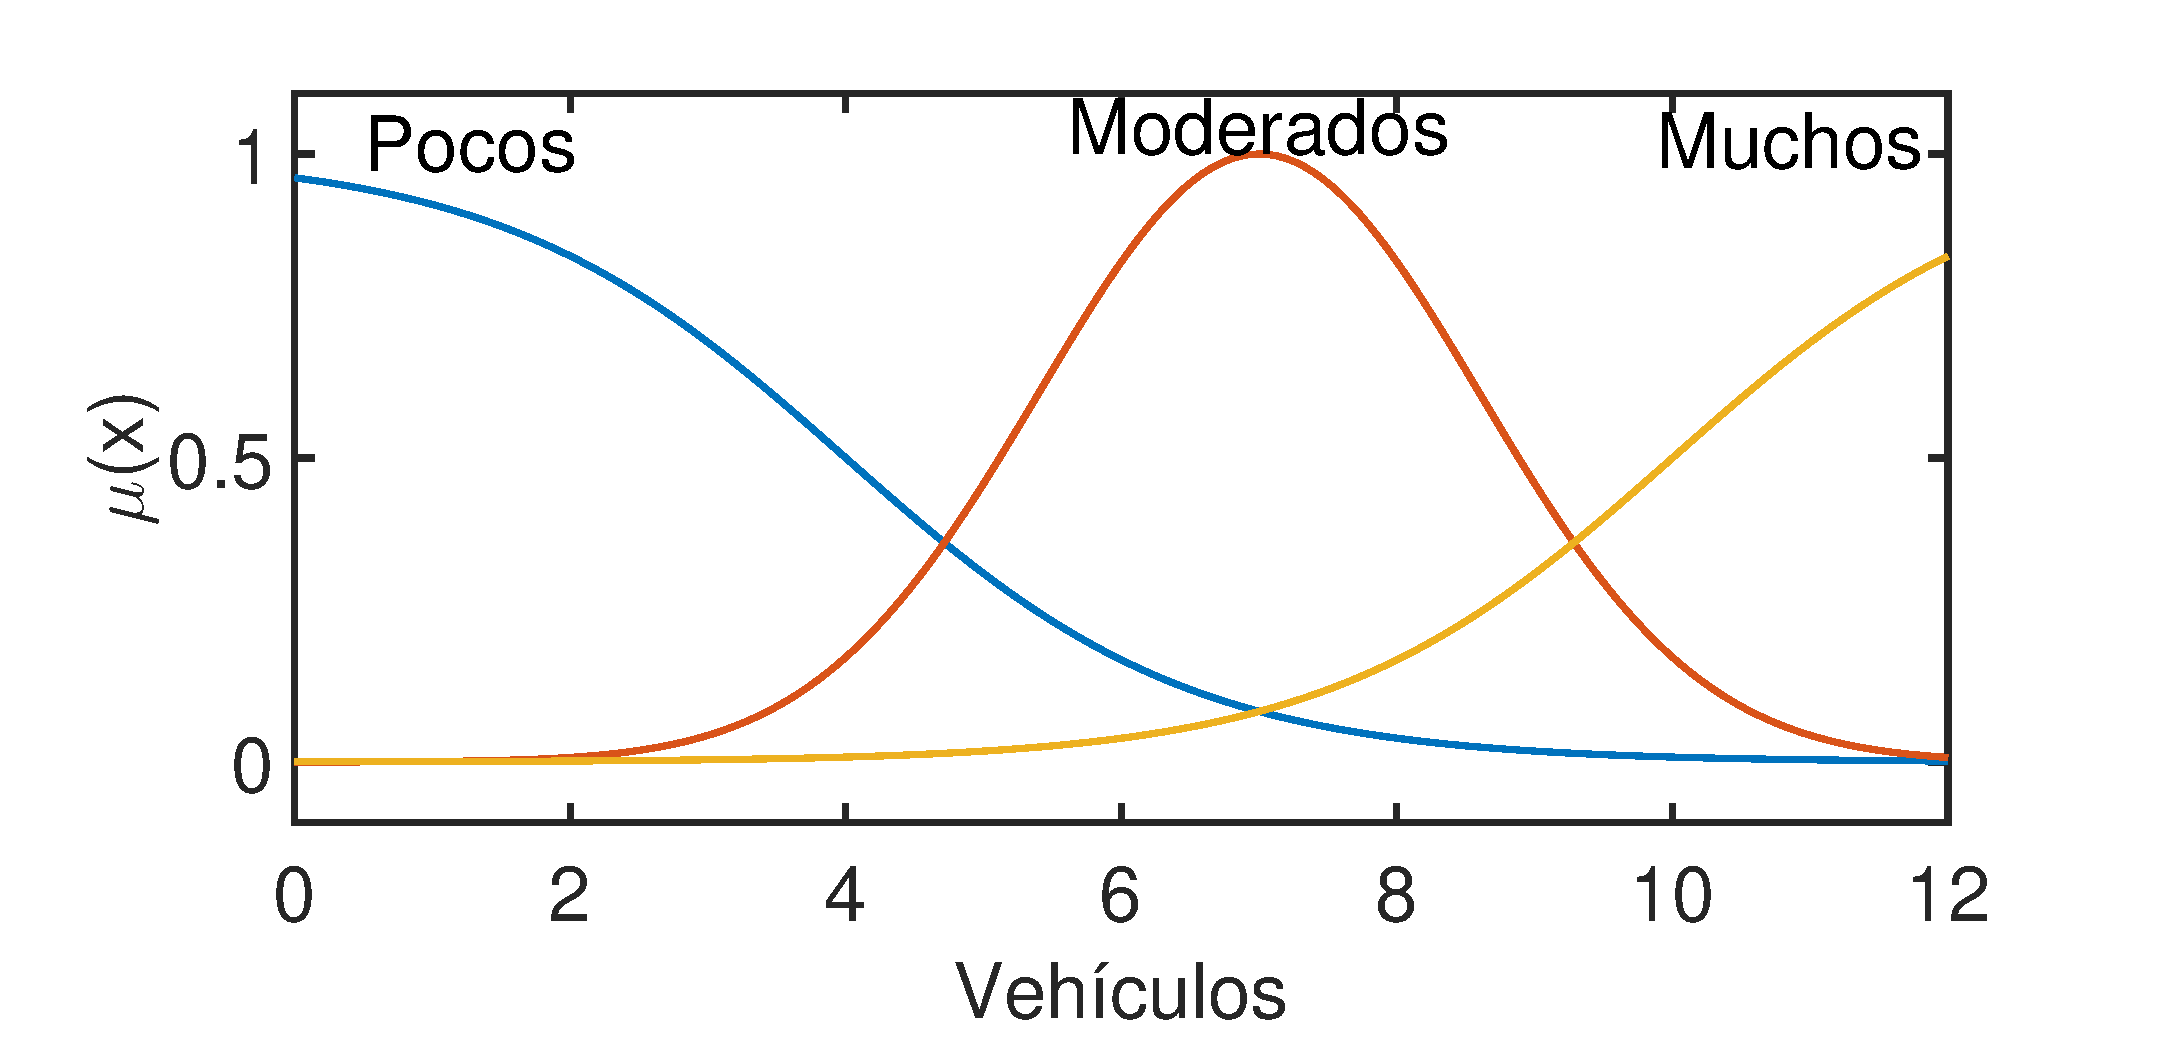
\includegraphics[height=4cm, width=8.1cm]{Variables/ConfigD_input1.eps}}
	\subfigure[Variable lingüística Congestión]{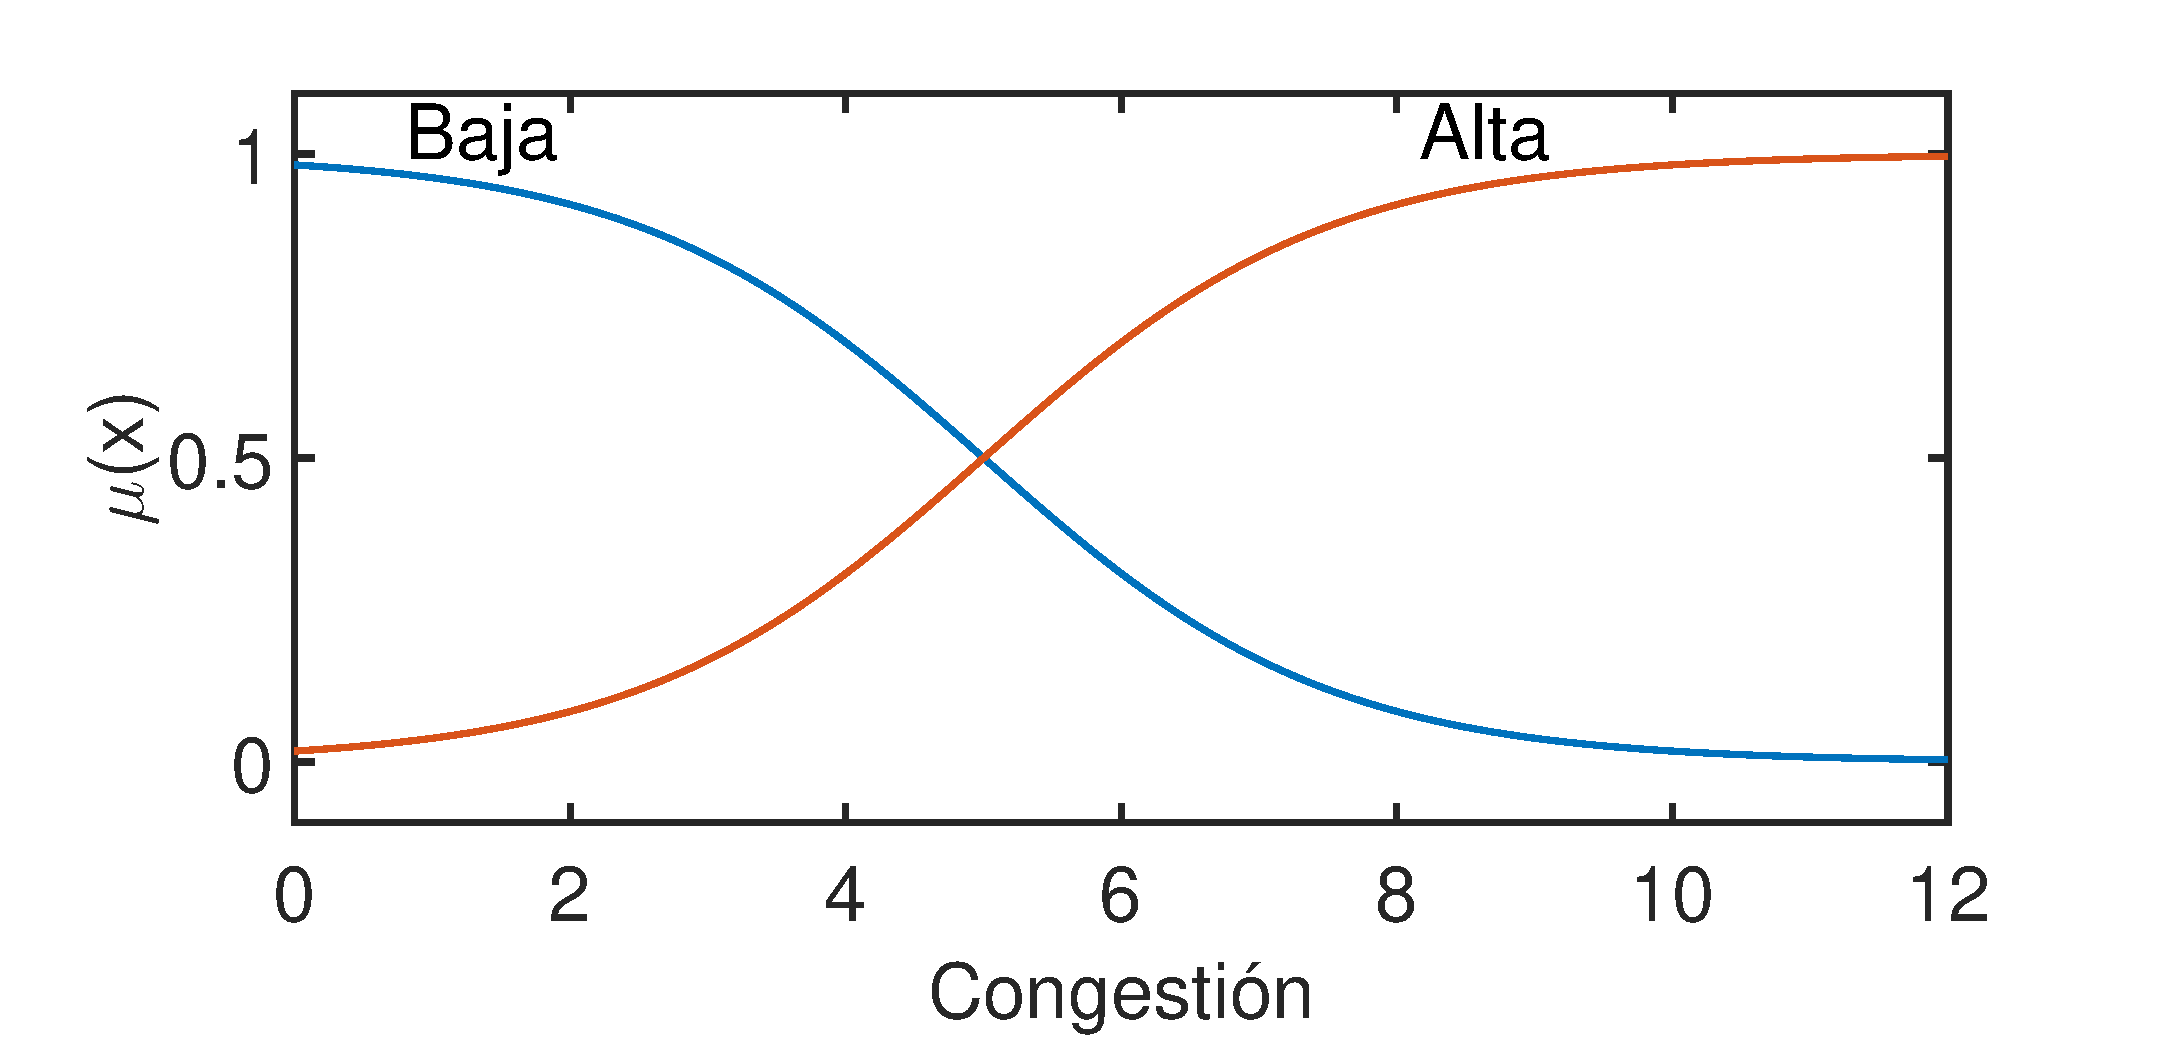
\includegraphics[height=4cm, width=8.1cm]{Variables/ConfigD_input2.eps}}
	\caption[Gráficas de las variables lingüísticas vehículos y congestión]{Representación gráfica de las variables lingüísticas Vehículos y Congestión }
\end{figure}

\textbf{Variable de salida Tiempo.} Esta variable únicamente tiene un ajuste menor en el término lingüístico \textit{Mínimo}, el resto de términos permanece intacto.

\begin{table}[!h]
	\centering
	\begin{tabular}{llr} \toprule
		Termino lingüístico & Función de membresía & Parámetros \\ \midrule
		Mínimo & Triangular & [0, 0, 25 ] \\
		Bajo & Triangular & [0, 25, 40 ] \\
		Medio & Triangular & [20, 40, 60] \\
		Alto & Triangular & [40, 60, 80] \\
		Extra & Triangular & [60, 80, 80] \\ \bottomrule
	\end{tabular}
	\caption{Variable lingüística \textit{Tiempo}}
\end{table}

\begin{figure}[H]
	\centering
	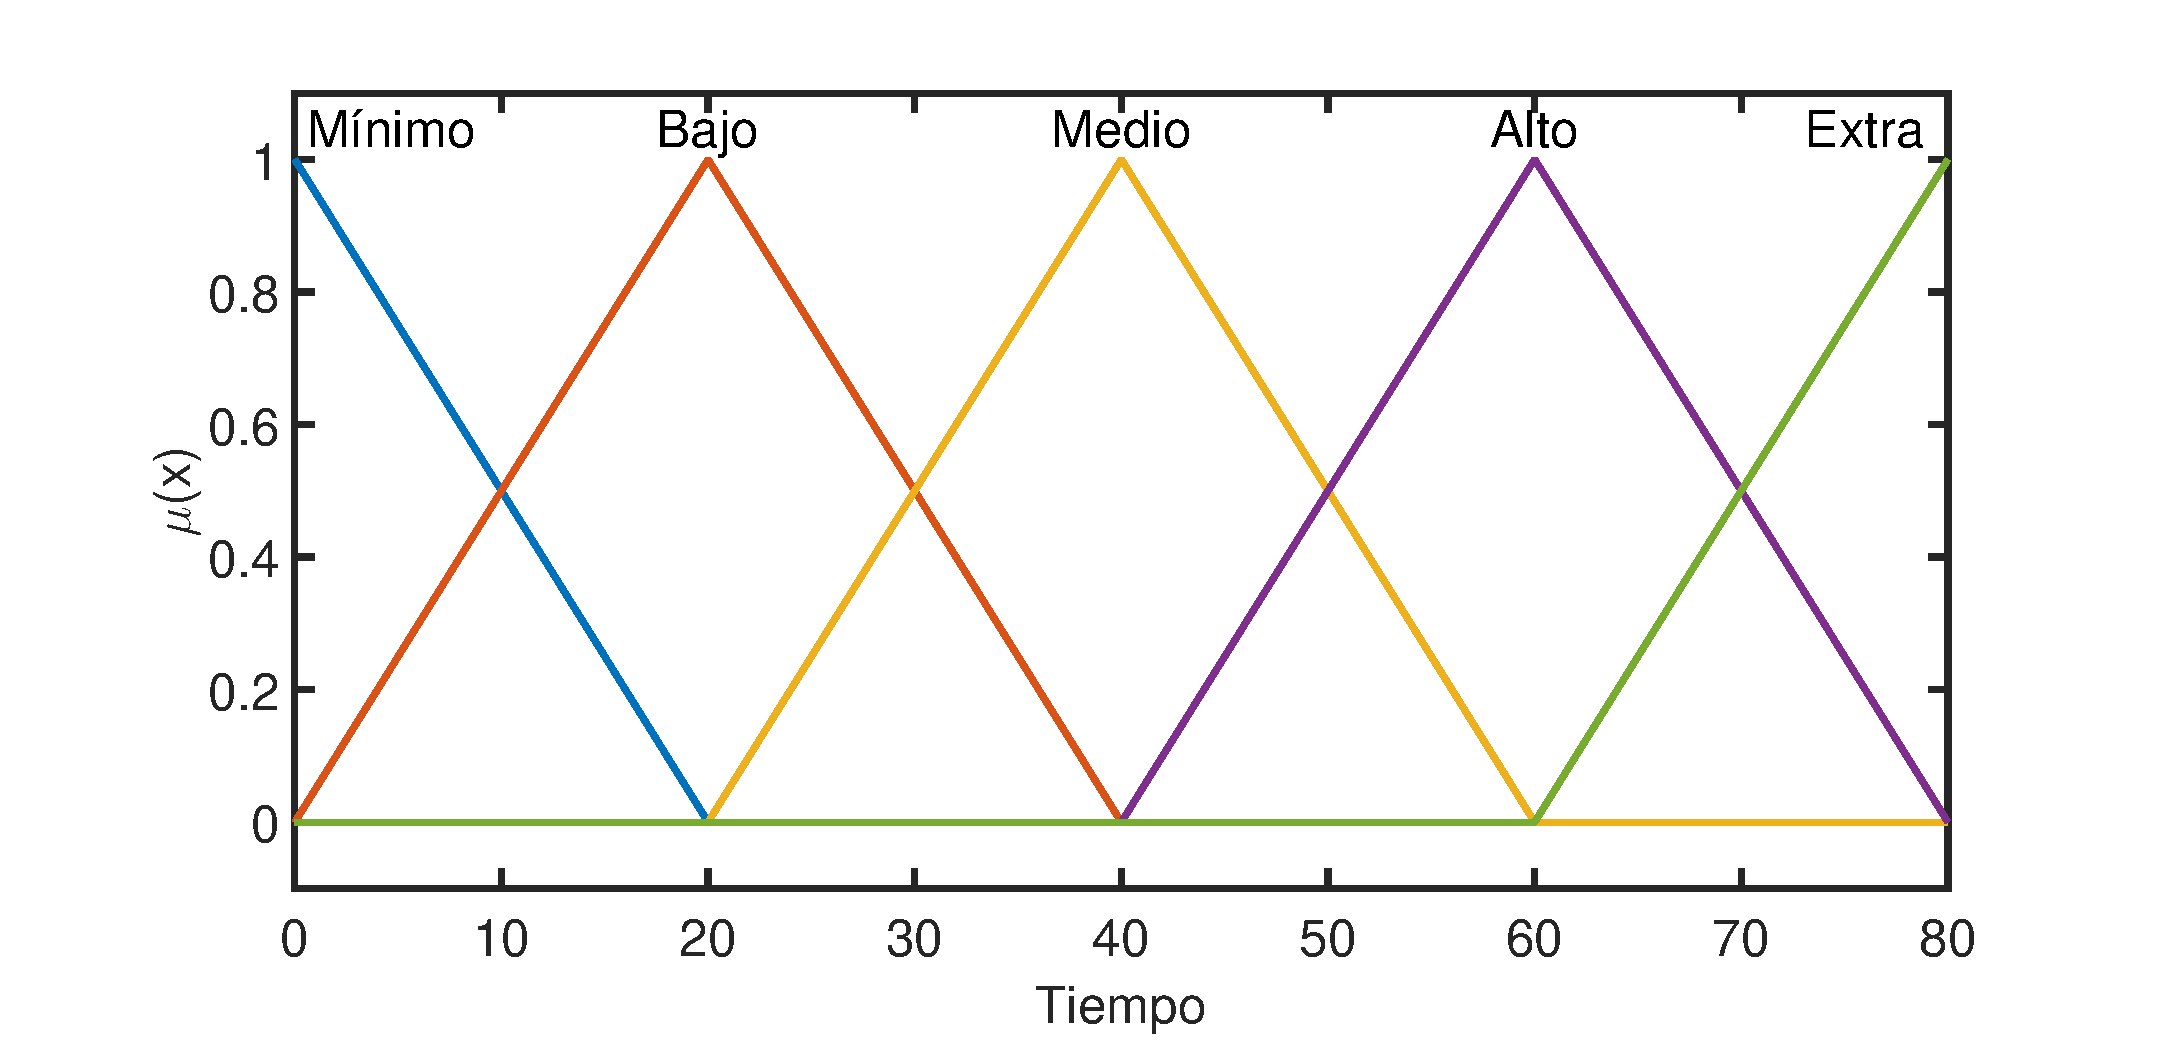
\includegraphics[height=5cm, width=12cm]{Variables/ConfigD_output1.eps}
	\caption[Gráfica variable lingüística tiempo - D]{Representación gráfica de la variable lingüística Tiempo}
\end{figure}

\subsubsection{Base de conocimientos}
La siguiente tabla muestra las reglas difusas empleadas en esta configuración que se mantiene sin cambios.
\begin{longtable}[c]{lclcl} \toprule
	\multicolumn{3}{c}{Antecedente} & & Consecuente \\ \midrule
	\multicolumn{3}{c}{Vehículos Pocos} & $\rightarrow$ & Verde Mínimo \\
	Vehículos Moderados & Y & Congestión Baja& $\rightarrow$ & Verde Medio \\
	Vehículos Moderados & Y & Congestión Alta& $\rightarrow$ & Verde Bajo \\
	Vehículos Muchos &Y& Congestión Baja& $\rightarrow$ & Verde Extra \\
	Vehículos Muchos &Y& Congestión Alta& $\rightarrow$ & Verde Alto \\ \hline
	\caption{Reglas difusas para la configuración \textit{D}}
\end{longtable}

\pagebreak
\subsubsection{Resultados}
Después de remplazar algunas de las funciones de membresía y realizar los ajustes necesarios, se le suministró los mismos valores de prueba para evaluar su desempeño respecto a la configuración anterior. Los resultados de dicha evaluación se reflejan en la tabla siguiente:

\begin{longtable}[c]{cccccc} \toprule
	$V \backslash C$ &  0 & 3 & 6 & 9 & 12 \\ \midrule
	0 & 08.41 & 08.41 & 08.41 & 08.41 & 08.41 \\
	3 & 13.25 & 13.25 & 13.25 & 12.98 & 10.85 \\
	6 & 36.56 & 36.54 & 28.81 & 24.08 & 24.02 \\
	9 & 47.81 & 43.60 & 39.23 & 37.65 & 37.62 \\
	12& 70.83 & 66.58 & 60.27 & 59.40 & 59.39 \\
	\caption{Resultados de la evaluación para la configuración \textit{D}}
\end{longtable}

Donde: la columna V son los valores de prueba de la variable Vehículos, la fila C son los valores de  prueba de la variable Congestión y las celdas son los tiempos (en segundos) obtenidos por la configuración actual.

\subsubsection{Observaciones}

\begin{multicols}{2}
	Definitivamente, los resultados obtenidos tras remplazar las funciones triangulares por funciones sigmoidales y gaussianas, son mucho más acertadas. Al principio, los tiempos asignados incrementan más rápido conforme más se eleva el número de autos, después, el ritmo de crecimiento de los tiempos de asignación desacelera al acercarse al valor máximo para las variables de entrada. Se concluye que la configuración actual será la usada en la implementación.
	\begin{figure}[H]
	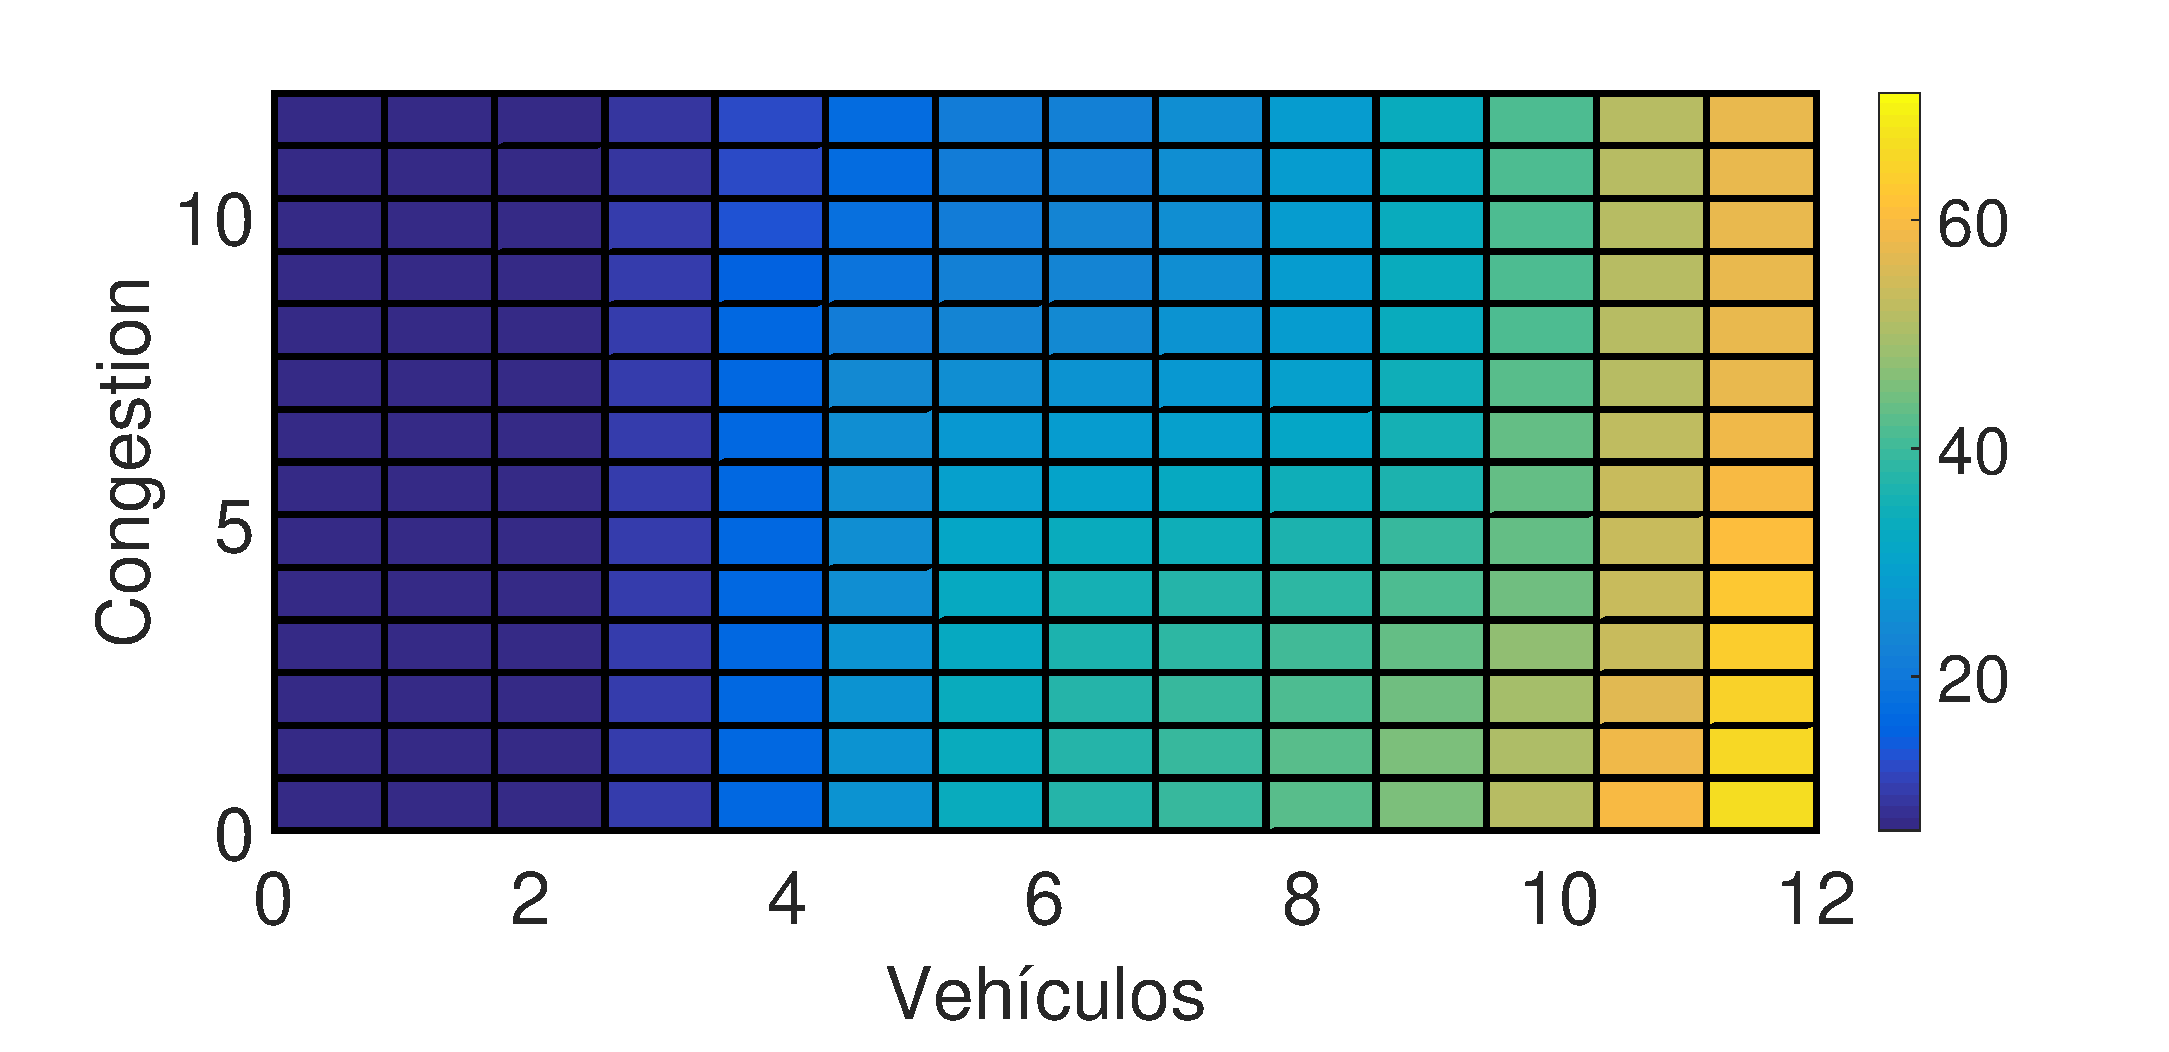
\includegraphics[width=0.5\textwidth]{Surfaces/Surface2D_D.eps}
	\caption{Superficie de control}
\end{figure}
\end{multicols}
\pagebreak

\section{Desarrollo del algoritmo}\label{section:desarrolloAlgoritmo}
Después de haber culminado el desarrollo del sistema de inferencia, el cual representa el componente principal del proyecto, ahora el desarrollo continúa con el algoritmo de sincronización de semáforos.

El modelo propuesto, es a su vez un marco de trabajo para la implementación última, por parte del usuario final.

A lo largo de las siguientes páginas se modela el desarrollo del algoritmo mediante diagramas UML, empleando solo aquellos diagramas que ayuden a tener una perspectiva general del proyecto:
\begin{itemize}
	\item \textbf{Diagrama de actividades} del flujo general del sistema.
	\item \textbf{Diagrama de clases} de todo el sistema.
	\item \textbf{Diagrama de secuencia} del bucle principal.
\end{itemize}

\begin{figure}[H]
	\centering
	\begin{tikzpicture}
	[node distance=10mm and 15mm,
	 legend/.style={pos=0.4, font=\scriptsize, fill=white},
	 block/.style={rectangle,draw=black,fill=yellow!20,thin,minimum height=10mm, minimum width=43mm, font=\footnotesize},
	 rline/.style={->, shorten >= 1pt, >= stealth', semithick,draw=black},]
	 	\node[block] (cam) {Sensor Vehiculos {\scriptsize (e.g. Cámara)} };
		\node[block] (in) [below=of cam] {Entradas {\scriptsize (e.g. Congestión)}};
		\node[block] (fis) [below=of in] {Sistema Difuso};
		\node[block] (out) [below=of fis] {Salidas {\scriptsize (e.g. Tiempo)}};
		\node[block] (sem) [below=of out] {Semáforo ``Inteligente''};

		\node[block] (rules) [left=of fis] {Reglas Difusas};
		\node[block] (vars) [right=of fis] {Variables Lingüísticas};

		\draw [rline] (cam) -- node[legend] {Pre-Procesamiento} (in);
		\draw [rline] (in) -- node[legend] {Fuzzificación} (fis);
		\draw [rline] (fis) -- node[legend] {Defuzzificación} (out);
		\draw [rline] (out) -- node[legend] {Post-Procesamiento} (sem);
		
		\draw [rline] (rules) -- (fis);
		\draw [rline] (vars) -- (fis);
	\end{tikzpicture}
	\caption{Diagrama general del sistema}
\end{figure}

\newpage
\subsection{Diagrama de actividades}
El siguiente diagrama muestra a grandes rasgos, el flujo de ejecución general del algoritmo. En él se puede observar el proceso de inicialización y configuración del semáforo y del sensor; además se muestra el bucle principal ``\emph{repetir siempre}'' que se encarga de obtener los datos del sensor, procesarlos y establecer el cambio de fase.

\begin{figure}[H]
	\centering
	\begin{tikzpicture}
		[auto,
		decision/.style	={diamond, draw=blue, thin, fill=yellow!20, text width=5cm, align=flush center, inner sep=1pt},
		bucle/.style	={chamfered rectangle, draw=black, thin, fill=yellow!20, text width=5.5cm, align=flush center, minimum height=2em},
		block/.style	={rectangle, draw=black, thin, fill=yellow!20, text width=5cm, align=center, minimum height=2em},
		line/.style		={draw=black, semithick, -latex', shorten >= 2pt},
		cloud/.style = {draw=red, thick, ellipse, fill=red!20, minimum height=2em}
		]
		\useasboundingbox (-8.3, 1) rectangle (9,-14);
		\scope[transform canvas={scale=.9}]
		\node at (-6.3cm,0) {Main};
		\node at (0,0) {Semáforo};
		\node at (6.3cm,0) {Sensor};
		
		\draw [dashed] (-3.25cm,0) -- +(0,-15cm);
		\draw [dashed] (3.25cm,0) -- +(0,-15cm);
		\draw (-9cm,0.5cm) rectangle (9cm,-15.1cm);
		\matrix[column sep=5mm, row sep=5mm, anchor=north] at (0,-1)
		{
			\node [block] (init)	{Inicio}; & &\\
			\node [block] (setupconfig)	{Inicializar Configuración}; & &\\
			\node [block] (setupsensor)	{Inicializar Sensor}; & &\\
			\node [block] (setupsemaforo)	{Inicializar Semáforo}; && \\
			\node [block] (runsemaforo) {Iniciar Semáforo}; & &\\
			& \node [bucle] (repetir) {Repetir siempre}; & \\
			& & \node [block] (contar) {Contar vehículos};\\
			& \node [block] (preprocesar)	{Preprocesar Datos}; & \\
			& \node [block] (inferir)	{Inferir Tiempo}; & \\
			& \node [block] (establecer)	{Establecer Fase}; & \\
		};

		\begin{scope}[every path/.style=line]
			\path	(init) -- (setupconfig);
			\path	(setupconfig) -- (setupsensor);
			\path	(setupsensor) -- (setupsemaforo);
			\path	(setupsemaforo) -- (runsemaforo);
			\path	(runsemaforo) -| (repetir);
			\path	(repetir) -| (contar);
			\path	(contar) |- (preprocesar);
			\path	(preprocesar) -- (inferir);
			\path	(inferir) -- (establecer);
			\path	(establecer) -- +(-6,0) |- (repetir);
		\end{scope}
		\endscope
	\end{tikzpicture}
	\caption{Diagrama de actividades general}
\end{figure}
\newpage


\subsection{Diagrama de secuencia}
\textbf{Diagrama de secuencia del bucle de control del semáforo}\\
En el diagrama anterior se muestra el bucle principal del sistema, ahora mediante un diagrama de secuencia se detallarán dicho bucle debido a que es la parte central del sistema.

Para fines de legibilidad, en el siguiente diagrama se omiten los nombres de las clases (\emph{FuzzySemaforo y SensorVehiculos}). Las funciones que se muestran pertenecen a la clase \emph{FuzzySemaforo} excepto una, la cual está indicada en el diagrama.
\begin{figure}[H]
	\centering
	\tikzumlset{font=\small, call dt=7, call padding=3.5}
	\begin{tikzpicture}

	\begin{umlseqdiag}[]
	\umlobject[]{run}
	\umlobject[x=5]{read}
	\umlobject[x=7.0]{getMedia}
	\umlobject[x=9.2]{getTime}
	\umlobject[x=11.4]{setLights}
	
	\begin{umlfragment}[type=loop, inner xsep=7]
	\begin{umlcall}[op=read(), return={autos : vector<int>}]{run}{read}\end{umlcall}
	\begin{umlcall}[op={get\_media(fase,vehiculos)}, return=vehículos : double]{run}{getMedia}\end{umlcall}
	\begin{umlcall}[op={get\_media(fase,congestión)}, return=congestión : double]{run}{getMedia}\end{umlcall}
	\begin{umlcall}[op=infiere tiempo en verde, return=segundos : double, name=call]{run}{getTime}\end{umlcall}
	\begin{umlcall}[op=establece la siguiente fase, return=void]{run}{setLights}\end{umlcall}
	\end{umlfragment}
	\umlnote[x=10, y=-3]{read}{Función miembro de la clase MySensor}
	%\umlnote[x=11, y=-6]{call-1}{Llamada al Sistema de Inferencia Difusa}
	\end{umlseqdiag}

	\end{tikzpicture}
	\caption{Diagrama de secuencia del bucle principal}	
\end{figure}


\subsection{Diagrama de clases}\label{subsection:umlclases}
\textbf{Modelado de las \textit{relaciones de clase} del sistema}\\
En el siguiente diagrama se modela las clases que constituyen el sistema además, se muestran las diferentes relaciones que existen entre dichas clases.

Para mayor legibilidad, el diagrama no modela atributos ni comportamientos de las clases; sin embargo, en el apéndice \ref{apendice:a} se modelan los elementos omitidos.
\begin{figure}[h]
\begin{tikzpicture}

\umlsimpleclass[y=-2.5]{MySemaforo}
\umlsimpleclass[x=-6.6, y=0]{FuzzySet}
\umlsimpleclass[x=6.5, y=-2.5]{MySensor}
\umlsimpleclass[type=abstract]{FuzzySemaforo}

\umlsimpleclass[x=-4, y=3.5]{TriangularMF}
\umlsimpleclass[x=0, y=3.5]{SigmoidalMF}
\umlsimpleclass[x=4, y=3.5]{GaussianaMF}

\umlsimpleclass[x=-6.6, y=7]{FuzzyValue}
\umlsimpleclass[x=0, y=7, type=abstract]{MembershipFunction}
\umlsimpleclass[x=6.5, y=7, type=abstract]{SensorVehiculos}

\umlunicompo[geometry=|-|, anchor1=140, mult1=1, mult2=0..*, pos2=2.8]{FuzzySemaforo}{TriangularMF}
\umlunicompo[geometry=|-|, anchor1=90, mult1=1, mult2=0..*, pos2=2.8]{FuzzySemaforo}{SigmoidalMF}
\umlunicompo[geometry=|-|, anchor1=40, mult1=1, mult2=0..*, pos2=2.8]{FuzzySemaforo}{GaussianaMF}

\umlunicompo[mult1=1, pos1=0, align1=right, mult2=0..*, pos2=1, align2=left]{FuzzySemaforo}{FuzzySet}
\umluniassoc[geometry=-|, anchor2=-130, attr2=cuenta vehículos|1, pos2=1, align2=right, align1=left, mult1=1, pos1=0]{FuzzySemaforo}{SensorVehiculos}
\umlimpl[geometry=|-|]{TriangularMF}{MembershipFunction}
\umlimpl[geometry=|-|]{SigmoidalMF}{MembershipFunction}
\umlimpl[geometry=|-|]{GaussianaMF}{MembershipFunction}

\umlimpl{MySensor}{SensorVehiculos}
\umluniassoc[mult1=1, pos1=0, align1=right, mult2=0..1, pos2=1, align2=left]{MembershipFunction}{FuzzyValue}
\umluniassoc[mult1=1, pos1=0.05, mult2=0..1, pos2=1, align2=left]{FuzzySet}{FuzzyValue}	

\umlimpl{MySemaforo}{FuzzySemaforo}
\end{tikzpicture}
\caption{Diagrama de clases del sistema}
\label{uml:relaciones}
\end{figure}
%\newpage
%\textbf{Diagrama de actividades que modela el proceso de inferencia}


\chapter{Conclusiones}

\section{Conclusiones del proyecto}
La Inteligencia Artificial juega un papel cada vez mas importante en nuestras vidas, desde los asistentes personales en nuestros móviles, hasta la optimización de procesos en la industria. Dentro de las diversas técnicas de IA, la Lógica Difusa, permite modelar situaciones del mundo real de una manera elegante, sencilla y fácil.

En este proyecto se abordó el problema de la congestión en los cruces semáforizados. Una de las principales causas de la congestión es la configuración de tiempos estáticos que a menudo ``desperdicia el tiempo'' en avenidas donde la cantidad de autos es nula o mínima.

La solución propuesta fue un Sistema de Inferencia Difusa que asignara tiempos de acuerdo a la cantidad de vehículos en las avenidas que se intersectan. El sistema fue capaz de reaccionar de manera adecuada frente a diversas situaciones. 

Cabe destacar que durante el diseño del FIS, no fue esencial conocer a fondo el modelo matemático de los semáforos, siendo esto uno de los principales atractivos de esta técnica de IA. Además, permitió definir el problema en jerga común, esto es, en términos coloquiales donde la imprecisión dificulta la asignación de rangos bien definidos a dichos términos.

En conclusión, la técnica seleccionada permitió dar solución al problema de una manera acertada. 
\section{Recomendaciones}
Aún queda un largo camino por recorrer, un proyecto multidisciplinario como este, necesita de diferentes expertos en diferentes áreas para tratar algunos detalles finos. Las recomendaciones que emitimos en pro de mejorar la eficacia del algoritmo son las siguientes:

\textbf{Acerca del ciclo del semáforo.}
Si bien, el sistema es capaz de asignar tiempos de manera dinámica en respuesta a la cantidad de vehículos en la intersección, sugerimos analizar la posibilidad de añadir una capa extra al sistema. Una capa encargada de determinar la longitud del ciclo. La salida de dicha capa extra sería un factor de multiplicación para alargar o acortar la duración del ciclo, y sus entradas podrían ser la longitud media de la cola de vehículos u otros factores como la hora pico o el clima, factores que afectan el tiempo de reacción de los automovilistas.

\textbf{Acerca del algoritmo de visión computacional.}
Para el conteo de automóviles en las avenidas, se recomienda el uso del algoritmo propuesto en \cite{ittap} cuya implementación en C++ facilitamos en el apéndice \ref{apendice:b}  por motivos de eficiencia y compatibilidad. 

Dicho trabajo arroja un algoritmo implementado en \emph{Python} que, según los resultados de la propia investigación, ha probado tener una eficacia (con buena iluminación) de hasta un 95\%.

El tiempo de ejecución del algoritmo sugerido por \textsc{estrada \& recinos \& vidal (2017)}: ``Detección de vehículos mediante imagen de fondo '' es de 1.5 segundos (implementado en Python), sin embargo al implementarse en C++ alcanza un tiempo de 0.03 segundos, es decir, 3 centésimas de segundo. Por lo que se recomienda el uso de este algoritmo implementado en C++.

\textbf{Mejoras.}
A tal algoritmo se le recomienda agregar una fase donde se compense la perspectiva desde la cual se tome la foto, ya que debido a esto, los autos más lejanos podrían no cubrir la cuota de pixeles mínima y por ende pasarían desapercibidos para el semáforo.


\chapter{Conclusiones}

\section{Conclusiones del proyecto}
La Inteligencia Artificial juega un papel cada vez mas importante en nuestras vidas, desde los asistentes personales en nuestros móviles, hasta la optimización de procesos en la industria. Dentro de las diversas técnicas de IA, la Lógica Difusa, permite modelar situaciones del mundo real de una manera elegante, sencilla y fácil.

En este proyecto se abordó el problema de la congestión en los cruces semáforizados. Una de las principales causas de la congestión es la configuración de tiempos estáticos que a menudo ``desperdicia el tiempo'' en avenidas donde la cantidad de autos es nula o mínima.

La solución propuesta fue un Sistema de Inferencia Difusa que asignara tiempos de acuerdo a la cantidad de vehículos en las avenidas que se intersectan. El sistema fue capaz de reaccionar de manera adecuada frente a diversas situaciones. 

Cabe destacar que durante el diseño del FIS, no fue esencial conocer a fondo el modelo matemático de los semáforos, siendo esto uno de los principales atractivos de esta técnica de IA. Además, permitió definir el problema en jerga común, esto es, en términos coloquiales donde la imprecisión dificulta la asignación de rangos bien definidos a dichos términos.

En conclusión, la técnica seleccionada permitió dar solución al problema de una manera acertada. 
\section{Recomendaciones}
Aún queda un largo camino por recorrer, un proyecto multidisciplinario como este, necesita de diferentes expertos en diferentes áreas para tratar algunos detalles finos. Las recomendaciones que emitimos en pro de mejorar la eficacia del algoritmo son las siguientes:

\textbf{Acerca del ciclo del semáforo.}
Si bien, el sistema es capaz de asignar tiempos de manera dinámica en respuesta a la cantidad de vehículos en la intersección, sugerimos analizar la posibilidad de añadir una capa extra al sistema. Una capa encargada de determinar la longitud del ciclo. La salida de dicha capa extra sería un factor de multiplicación para alargar o acortar la duración del ciclo, y sus entradas podrían ser la longitud media de la cola de vehículos u otros factores como la hora pico o el clima, factores que afectan el tiempo de reacción de los automovilistas.

\textbf{Acerca del algoritmo de visión computacional.}
Para el conteo de automóviles en las avenidas, se recomienda el uso del algoritmo propuesto en \cite{ittap} cuya implementación en C++ facilitamos en el apéndice \ref{apendice:b}  por motivos de eficiencia y compatibilidad. 

Dicho trabajo arroja un algoritmo implementado en \emph{Python} que, según los resultados de la propia investigación, ha probado tener una eficacia (con buena iluminación) de hasta un 95\%.

El tiempo de ejecución del algoritmo sugerido por \textsc{estrada \& recinos \& vidal (2017)}: ``Detección de vehículos mediante imagen de fondo '' es de 1.5 segundos (implementado en Python), sin embargo al implementarse en C++ alcanza un tiempo de 0.03 segundos, es decir, 3 centésimas de segundo. Por lo que se recomienda el uso de este algoritmo implementado en C++.

\textbf{Mejoras.}
A tal algoritmo se le recomienda agregar una fase donde se compense la perspectiva desde la cual se tome la foto, ya que debido a esto, los autos más lejanos podrían no cubrir la cuota de pixeles mínima y por ende pasarían desapercibidos para el semáforo.


% Apendices
\appendix
\chapter{Diagramas de clases UML}\label{apendice:a}
En la sección \ref{subsection:umlclases}, página \pageref{subsection:umlclases} se mostró el siguiente diagrama UML con elementos omitidos, ahora se presentarán el resto de diagramas completos.

\begin{figure*}[h]
	\begin{tikzpicture}
	
	\umlsimpleclass[y=-2.5]{MySemaforo}
	\umlsimpleclass[x=-6.6, y=0]{FuzzySet}
	\umlsimpleclass[x=6.5, y=-2.5]{MySensor}
	\umlsimpleclass[type=abstract]{FuzzySemaforo}
	
	\umlsimpleclass[x=-4, y=3.5]{TriangularMF}
	\umlsimpleclass[x=0, y=3.5]{SigmoidalMF}
	\umlsimpleclass[x=4, y=3.5]{GaussianaMF}
	
	\umlsimpleclass[x=-6.6, y=7]{FuzzyValue}
	\umlsimpleclass[x=0, y=7, type=abstract]{MembershipFunction}
	\umlsimpleclass[x=6.5, y=7, type=abstract]{SensorVehiculos}
	
	\umlunicompo[geometry=|-|, anchor1=140, mult1=1, mult2=0..*, pos2=2.8]{FuzzySemaforo}{TriangularMF}
	\umlunicompo[geometry=|-|, anchor1=90, mult1=1, mult2=0..*, pos2=2.8]{FuzzySemaforo}{SigmoidalMF}
	\umlunicompo[geometry=|-|, anchor1=40, mult1=1, mult2=0..*, pos2=2.8]{FuzzySemaforo}{GaussianaMF}
	
	\umlunicompo[mult1=1, pos1=0, align1=right, mult2=0..*, pos2=1, align2=left]{FuzzySemaforo}{FuzzySet}
	\umluniassoc[geometry=-|, anchor2=-130, attr2=cuenta vehículos|1, pos2=1, align2=right, align1=left, mult1=1, pos1=0]{FuzzySemaforo}{SensorVehiculos}
	\umlimpl[geometry=|-|]{TriangularMF}{MembershipFunction}
	\umlimpl[geometry=|-|]{SigmoidalMF}{MembershipFunction}
	\umlimpl[geometry=|-|]{GaussianaMF}{MembershipFunction}
	
	\umlimpl{MySensor}{SensorVehiculos}
	\umluniassoc[mult1=1, pos1=0, align1=right, mult2=0..1, pos2=1, align2=left]{MembershipFunction}{FuzzyValue}
	\umluniassoc[mult1=1, pos1=0.05, mult2=0..1, pos2=1, align2=left]{FuzzySet}{FuzzyValue}	
	
	\umlimpl{MySemaforo}{FuzzySemaforo}
	\end{tikzpicture}
	\caption{Diagrama de clases que muestra las relaciones del sistema}
	\label{uml:relaciones2}
\end{figure*}
\newpage

\section{Diagramas de las clases \textit{FuzzySet y FuzzyValue}}

\begin{figure}[H]
	\centering
	\begin{tikzpicture}
	
	\umlclass[anchor=north, y=-4]
	{FuzzySet}
	{- set\_u : vector< double > \\- set\_x : vector< double >}
	{+ FuzzySet( begin : double, step : double, end : double )\\
		+ FuzzySet( set : FuzzySet, f : MembershipFunction)\\
		+ operator>>( a : FuzzySet, b : FuzzySet) : FuzzySet\\
		+ operator\&( a : FuzzySet, b : FuzzySet) : FuzzySet\\
		%  	 + Print(show\_cero : bool ) : void \\
		+ get\_centroid() : double}
	
	\umlclass[]
	{FuzzyValue}
	{- x : double}
	{+ FuzzyValue( x : double) \\
		+ FuzzyValue( v : FuzzyValue)\\
		+ operator\_double() : double\\
		+ operator=( v : FuzzyValue) : FuzzyValue\\
		+ operator\&( v : FuzzyValue ) : FuzzyValue}
	\end{tikzpicture}
	\caption{Diagrama de las clases \emph{FuzzySet} y \emph{FuzzyValue}}
\end{figure}
\newpage

\section{Jerarquía de herencia \textit{MembershipFunction}}
El siguiente diagrama UML modela los miembros de las clases \textit{MembershipFunction, TriangularMF, SigmoidalMF, GaussianaMF}, además muestra su relación de herencia.


\begin{figure}[h]
	\centering
	\begin{tikzpicture}
	\umlclass[type=abstract]{MembershipFunction}{}{\umlvirt{+ operator()( x : double ) : FuzzyValue}}
	
	\umlclass[x=8.1, y=5]
	{TriangularMF}
	{- a : double\\- b : double\\- c : double}
	{+ TriangularMF( a : double, b : double, c : double )\\+ operator()( x : double ) : FuzzyValue }
	
	\umlclass[x=9, y=0]
	{SigmoidalMF}
	{- a : double\\- $x_0$ : double}
	{+ SigmoidalMF( a : double, $x_0$ : double )\\+ operator()( x : double ) : FuzzyValue }
	
	\umlclass[x=9, y=-5]
	{GaussianaMF}
	{- a : double\\- $x_0$ : double}
	{+ GaussianaMF( a : double, $x_0$ : double )\\+ operator()( x : double ) : FuzzyValue }
	
	\umlimpl[geometry=-|]{TriangularMF}{MembershipFunction}
	\umlimpl[]{SigmoidalMF}{MembershipFunction}
	\umlimpl[geometry=-|]{GaussianaMF}{MembershipFunction}
	\end{tikzpicture}
	\caption{Diagrama de clases que modela la jerarquía de herencia MembershipFunction }
\end{figure}


\newpage
\section{Realización de la clase \textit{SensorVehiculos}}
El siguiente diagrama modela los elementos omitidos de las clases \textit{SensorVehiculos} y \textit{MySensor}, además, se modela su relación de herencia y \emph{realización}.\\

\begin{figure}[h]
	\centering
	\begin{tikzpicture}
	\umlclass[type=abstract]
	{SensorVehiculos}
	{}
	{\umlvirt{+ read() : vector< double >} }
	
	\umlclass[y=-5]
	{MySensor}
	{ - num\_camaras : int }
	{ + SensorGenerico( camaras : int ) \\ + read() : vector< double > }
	
	\umlimpl[]{MySensor}{SensorVehiculos}
	
	\umlnote[x=-7, y=-5, anchor2=-160, width=4cm]{MySensor}{Esta clase es solo para demostración, deberá ser implementada adecuadamente por el usuario final }
	\end{tikzpicture}
	\caption{Diagrama de clases que modela la implementación de \textit{SensorVehiculos:read()}}
\end{figure}


\newpage
\section{Realización de la clase \textit{FuzzySemaforo}}
El siguiente diagrama modela los elementos omitidos de las clases \textit{FuzzySemaforo} y \textit{MySemaforo}, además, se modela su relación de herencia y \emph{realización}.\\

\begin{figure}[H]
	\centering
	\begin{tikzpicture}
	\umlclass[type=abstract]
	{FuzzySemaforo}
	{- num\_fases : int\\
		- num\_carriles : int\\
		- num\_avenidas : int\\
		- fase : int \\
		- tiempo : double\\
		- vehiculos : double\\
		- congestion : double\\
		- autos : vector< double >\\
		- pesos : vector< double >\\
		- ciclo : Ciclo\\
		- carriles : Carril\\
		- sensor : SensorVehiculos}
	{+ FuzzySemaforo( ciclo:Ciclo, carril:Carril, sensor:SensorVehiculos )\\
		+ run() : void\\
		\umlvirt{+ set\_lights( fase : int, tiempo : double ) : void}\\
		- get\_time( t : int, c : int) : double\\
		- get\_media( fase : int, estado : int)}	
	
	\umlclass[y=-9]{MySemaforo}{}
	{+ MySemaforo(ciclo:Ciclo, carriles:carril, sensor:SensorVehiculos)\\
		+ set\_lights( fase : int, tiempo : double) : void}
	
	\umlimpl{MySemaforo}{FuzzySemaforo}
	\umlnote[x=-8, y=-9, width=3cm]{MySemaforo}{Esta clase es solo para demostración, deberá ser implementada adecuadamente por el usuario final }
	\end{tikzpicture}
	\caption{Diagrama de clases que modela la implementación de \textit{set\_lights: FuzzySemaforo}}
\end{figure}

\chapter[Algoritmo de detección de vehículos]{Implementación en C++ de un algoritmo de detección de vehículos}\label{apendice:b}
Del resultado de la investigación realizada en \cite{ittap} se rescata el algoritmo de visión computacional seleccionado para la detección de automóviles. Dicho trabajo arroja un algoritmo implementado en \emph{Python} que, según los resultados de la propia investigación, ha probado tener una eficacia (con buena iluminación) de hasta un 95\%.

El tiempo de ejecución del algoritmo sugerido por \emph{Estrada \& Recinos \& Vidal (2017)}: ``Detección de vehículos mediante imagen de fondo '' es de 1.5 segundos (implementado en Python), sin embargo al implementarse en C++ alcanza un tiempo de 0.03 segundos, es decir, 3 centésimas de segundo. 

\textbf{Requerimientos}\\
El algoritmo en su versión C++ requiere de un compilador que soporte el estándar ISO C++11 además de tener compilado e instalado la librería para visión por computadora OpenCV en su versión 2.x. \\\\
\textbf{Código Fuente}\\
\lstinputlisting[
style=ezam,
caption={[Implementación en C++] Implementación en C++ del algoritmo de detección de vehículos}
]{algoritmo.cpp}


% Bibliografia
\begin{thebibliography}{99}
	
	\bibitem{garciag} García, G. (2017). Un enfoque de semáforo inteligente utilizando algoritmos de visión computacional en una intersección aislada para optimizar el flujo vehicular (Tesis de maestría). Centro de Investigación en Inteligencia Artificial (CIIA) de la Universidad Veracruzana, Xalapa de Enríquez, Veracruz, México. 
	
	\bibitem{alvaroer} Alvaro E., R. De Somocurcio S. (2008). Control de tráfico vehicular automatizado utilizando Lógica Difusa. Universidad Ricardo Palma, Lima, Perú.
	
	\bibitem{bencesramos} Bances, M., Ramos, M. (2014). Semáforos Inteligentes para la regulación del tráfico vehicular. Rev. Ingeniería: Ciencia, Tecnología e Innovación. Vol. 1 (No. 1). pp. 37-45. .
	
	\bibitem{MoraleslGonzales} Morales, L. Rafael., Gonzáles, S. Juan. (2013) \emph{Control de tráfico vehicular por medio de semáforos inteligentes}. Universidad de Rafael Urdaneta, República Bolivariana de Venezuela.  
	
	\bibitem{Hernandezca} Hernández, C.A., Salcedo, O., \& Pedraza, L.F. (2007). Modelo de Semaforización Inteligente para la Ciudad de Bogotá. Revista Científica y Tecnológica de la Facultad de Ingeniería, Universidad Distrital Francisco José de Caldas, Vol. 11(No.2). 61-69. 
	
	\bibitem{ittap} Estrada, E.K., Recinos, H., \& Vidal, G. Y. (2017). Selección de un algoritmo de visión por computadora para la detección de vehículos. Instituto Tecnológico de Tapachula, Tapachula, Chiapas, México.
	
	\bibitem{duarte} Oscar G. Duarte (1999). Sistemas de lógica difusa. Fundamentos. \textit{Revista Ingeniería e Investigación, No. 42, pp. 22.}
	
	\bibitem{sedesolpa} Secretaría de Desarrollo Social (SEDESOL). (1994). Programa de Asistencia técnica en transporte urbano para las ciudades medias mexicanas. Manual Normativo, Tomo XII. Estudios de Ingeniería de Tránsito. México.
	
	\bibitem{minusterioti} Ministerio de Transporte e Infraestructura. (2008). Manual para la Revisión de Estudios de Tránsito. Realización de Manuales Técnicos para la Revisión y Aprobación de Estudios y Diseños de Carreteras. Managua, Nicaragua.
	
	\bibitem{arandia} Juan Gabriel Tapia Arandia, Romel Daniel Veizaga Balta (2006).
		\emph{Apoyo didáctico para la enseñanza y aprendizaje de la asignatura de ingeniería de tráfico}.
		(Trabajo para optar al diploma de Licenciatura en Ingeniería Civil).
		Universidad Mayor De San Simón, Cochabamba, Bolivia.
	
	\bibitem{zadehfs} Zadeh, A.L. (1965). Fuzzy sets \emph{Information and Control}, vol. 8, pp. 338-353.
	
	\bibitem{zadehnewapproach} Zadeh, A.L. (1973). Outline of a New Approach to the Analysis of Complex Systems and Decision Processes. \emph{IEEE Transactions on Systems, Man, and Cybernetics}, Vol. SMC-3, (No. 1). 28-44.
	
	\bibitem{zadehlinguisticv} Zadeh, A.L. (1975). The Concept of a Linguistic Variable and its Application to Approximate Reasoning-I. \emph{Information Sciences}. Vol. 8. 199-249.
	
	\bibitem{ponce} Ponce Cruz P. (Primera Edición). (2010).
		\emph{Inteligencia Artificial con Aplicaciones a la Ingeniería}. México: Alfaomega.
	
	\bibitem{amador} Amador Hidalgo L. (Primera Edición). (1997).
		\emph{Inteligencia Artificial y Sistemas Expertos}. Córdoba: Universidad de Córdoba.
		
	\bibitem{alfonsovr2013} Alfonso V. Rivera. (2013). \emph{Controladores difusos aplicados a convertidores DC/DC} (Tesis de maestría). Universidad Autónoma de Aguascalientes, Aguascalientes, Ags.
	
	\bibitem{carlosgm} Carlos G. Morcillo. \emph{Lógica Difusa, una introducción práctica}. E-mail: Carlos.Gonzales@uclm.es
	
	\bibitem{josecarlos} José Carlos. \emph{Control Neuro-Difuso Aplicado a una Grúa Torre}. Recuperado de Tesis Digitales UNMSM
	
	\bibitem{kevinstephe} Kevin M. Passino, Stephen Yurkovick, (1997). \emph{Fuzzy Control}. California, Berkeley: ADDISON-WESLEY
	
	\bibitem{MarinIA} Marín, M. R., Palma, M. J. (2008). Inteligencia Artificial: Métodos, técnicas y aplicaciones. España: Mcgraw-Hill/Interamericana De España, S. A. U.
	\bibitem{IssaiGalvan} Isasi, V. P., Galván, L. I. (2004). Redes de Neuronas Artificiales: Un enfoque práctico. Madrid, España: Pearson Educación, S.A.
	
\end{thebibliography}



\end{document}